\documentclass[a4paper]{book}
\usepackage{a4wide}
\usepackage{makeidx}
\usepackage{graphicx}
\usepackage{multicol}
\usepackage{float}
\usepackage{listings}
\usepackage{color}
\usepackage{textcomp}
\usepackage{alltt}
\usepackage{times}
\usepackage{ifpdf}
\ifpdf
\usepackage[pdftex,
            pagebackref=true,
            colorlinks=true,
            linkcolor=blue,
            unicode
           ]{hyperref}
\else
\usepackage[ps2pdf,
            pagebackref=true,
            colorlinks=true,
            linkcolor=blue,
            unicode
           ]{hyperref}
\usepackage{pspicture}
\fi
\usepackage[utf8]{inputenc}
\usepackage{doxygen}
\lstset{language=C++,inputencoding=utf8,basicstyle=\footnotesize,breaklines=true,breakatwhitespace=true,tabsize=8,numbers=left }
\makeindex
\setcounter{tocdepth}{3}
\renewcommand{\footrulewidth}{0.4pt}
\begin{document}
\hypersetup{pageanchor=false}
\begin{titlepage}
\vspace*{7cm}
\begin{center}
{\Large PhysGameEngine \\[1ex]\large .01 }\\
\vspace*{1cm}
{\large Generated by Doxygen 1.6.3}\\
\vspace*{0.5cm}
{\small Fri May 14 09:49:04 2010}\\
\end{center}
\end{titlepage}
\clearemptydoublepage
\pagenumbering{roman}
\tableofcontents
\clearemptydoublepage
\pagenumbering{arabic}
\hypersetup{pageanchor=true}
\chapter{Physgame}
\label{index}\hypertarget{index}{}The Physgame engine is an abstraction layer between less portable, less user friendly, more sophistciated libraries and the game you want to make. If we do our jobs right this will save time and effort making and porting games between a variety of platforms. If you link only against this library, not a single line of your Standard compliant C++ code should need to change between platforms. At this early stage we are proving the concept with \char`\"{}Catch!\char`\"{} our first sample game. It Currently runs on Linux, Windows and Mac OS X with an Identical codebase, when we are done with \char`\"{}Catch!\char`\"{} We want it to have one codebase, and downloadable in the Iphone app store, on the PS3, Wii downloadon Steam, and in a variety of linux repositories.

To get the latest news on development checkout: \href{http://gitorious.org/physgame}{\tt http://gitorious.org/physgame} Or check the webpage \href{http://www.blacktoppstudios.com}{\tt http://www.blacktoppstudios.com}\hypertarget{index_Engine}{}\section{Structure}\label{index_Engine}
\hyperlink{mainloop1}{Main Loop Flow}

\hyperlink{classphys_1_1World}{World -\/ It integrates everything}

\hyperlink{classphys_1_1EventManager}{Events -\/ Handling messages, event and interupts from the outisde}

\hyperlink{actorcontainer1}{Actor Container -\/ Keeping track of our in game objects}\hypertarget{index_Types}{}\section{Data Types}\label{index_Types}
\hyperlink{classphys_1_1Vector3}{phys::Vector3}

\hyperlink{classphys_1_1Vector3WActor}{phys::Vector3WActor}

\hyperlink{classphys_1_1Ray}{phys::Ray}

\hyperlink{namespacephys_af7eb897198d265b8e868f45240230d5f}{phys::Real}

\hyperlink{namespacephys_a460f6bc24c8dd347b05e0366ae34f34a}{phys::Whole}

\hyperlink{classphys_1_1Quaternion}{phys::Quaternion}

\hyperlink{classphys_1_1MetaCode}{phys::MetaCode}\hypertarget{index_Classes}{}\section{Sophisticated Data Types}\label{index_Classes}
\hyperlink{classphys_1_1ActorBase}{Actors -\/ Items in the world}

\hyperlink{classphys_1_1EventBase}{phys::EventBase}

\hyperlink{classphys_1_1GraphicsManager}{phys::GraphicsManager}\hypertarget{index_Optional}{}\section{Optional Engine Components}\label{index_Optional}
\hyperlink{classphys_1_1WorldQueryTool}{phys::WorldQueryTool} 
\chapter{Main Loop Structure and Flow}
\label{mainloop1}
\hypertarget{mainloop1}{}
\begin{Desc}
\item[\hyperlink{todo__todo000033}{Todo}]create a lighting manager and put this in there \end{Desc}


The MainLoop is heart of most video games and simulations.\hypertarget{mainloop1_mainloopoverview1}{}\subsection{Main loop Overview}\label{mainloop1_mainloopoverview1}
The Main loop runs in \hyperlink{classphys_1_1World_af1d9e36d43f5e50543fa2351a32c8362}{World.MainLoop()} which is called by default from \hyperlink{classphys_1_1World_a21cc36be08a61f40619584d4c438936b}{World::GameInit()}. By default this Method also starts the render, the physics andthe input systems. It does very little on it's own. The main loop then calls the PreMainLoopItems(), DoMainLoopItems and PreMainLoopItems(), for each manager in the order of their priority from Lowest to Highest. \par
 Here is a listing of default priorities for each of the managers the a world intantiates by default: -\/50 User Input and events -\/40 Actors -\/30 Physics -\/20 \hyperlink{classphys_1_1Camera}{Camera} -\/10 Lighting (Not yet implemented) 0 Graphics 10 \hyperlink{classphys_1_1Sound}{Sound} 20 Resources 
\chapter{Todo List}
\label{todo}
\hypertarget{todo}{}
\label{dd/da0/todo__todo000034}
\hypertarget{dd/da0/todo__todo000034}{}
 
\begin{DoxyDescription}
\item[Page \hyperlink{mainloop1}{Main Loop Structure and Flow} ]create a lighting manager and put this in there 
\end{DoxyDescription}

\label{dd/da0/todo__todo000001}
\hypertarget{dd/da0/todo__todo000001}{}
 
\begin{DoxyDescription}
\item[Member \hyperlink{classphys_1_1ActorRigid_aab4a408ce0724be6adf4c9f51f55f8a1}{phys::ActorRigid::CreateShapeFromMeshDynamic}(short unsigned int accuracy=1) ]-\/ Check for thread safety 
\end{DoxyDescription}

\label{dd/da0/todo__todo000002}
\hypertarget{dd/da0/todo__todo000002}{}
 
\begin{DoxyDescription}
\item[Member \hyperlink{classphys_1_1ActorRigid_a84554dcaaf2475ba0ec7dcb9235050ac}{phys::ActorRigid::CreateShapeFromMeshStatic}() ]-\/ Check for thread safety 
\end{DoxyDescription}

\label{dd/da0/todo__todo000003}
\hypertarget{dd/da0/todo__todo000003}{}
 
\begin{DoxyDescription}
\item[Member \hyperlink{classphys_1_1ActorTerrain_a2403c40af6799e67c9aff1520b02dc0b}{phys::ActorTerrain::CreateShapeFromMeshStatic}() ]-\/ Check for thread safety 
\end{DoxyDescription}

\label{dd/da0/todo__todo000004}
\hypertarget{dd/da0/todo__todo000004}{}
 
\begin{DoxyDescription}
\item[Member \hyperlink{namespacephys_1_1crossplatform_a11ab7359564519dc966f997c98109f6e}{phys::crossplatform::RenderPhysWorld}(World $\ast$TheWorld, Ogre::RenderWindow $\ast$TheOgreWindow) ]Are seperate methods nessessary? Simple investigation showed that the same update() method is called when rendering one frame, but for all targets. 
\end{DoxyDescription}

\label{dd/da0/todo__todo000009}
\hypertarget{dd/da0/todo__todo000009}{}
 
\begin{DoxyDescription}
\item[Member \hyperlink{classphys_1_1EventManager_a018b36588bf2a2e90536e64be060d6fc}{phys::EventManager::EventManager}() ]TODO build a deconstructor that deletes all the events still in the queue 

TODO: Make the EventManager completely thread safe. IF this is completely thread safe, we can spawn numerous individual thread each accessing this and and the performance gain would almost scale directly with cpu core count increases. Look at boost scoped\_\-lock 
\end{DoxyDescription}

\label{dd/da0/todo__todo000007}
\hypertarget{dd/da0/todo__todo000007}{}
 
\begin{DoxyDescription}
\item[Member \hyperlink{classphys_1_1EventManager_a63cf23dc9fe0ced3e2c60ca61c97b166}{phys::EventManager::UpdateEvents}() ]There has got to be a more efficient way to do UpdateEvents() 
\end{DoxyDescription}

\label{dd/da0/todo__todo000008}
\hypertarget{dd/da0/todo__todo000008}{}
 
\begin{DoxyDescription}
\item[Member \hyperlink{classphys_1_1EventManager_a0cf574c55def063d66d7db46a4d3e8a5}{phys::EventManager::UpdateSystemEvents}() ]make Physevents for each of the events in SDL\_\-WmEvents(and delete the SDL events) 
\end{DoxyDescription}

\label{dd/da0/todo__todo000011}
\hypertarget{dd/da0/todo__todo000011}{}
 
\begin{DoxyDescription}
\item[Member \hyperlink{classphys_1_1GraphicsManager_aafcf1824190e44d42a9bfbea9cfbe1b2}{phys::GraphicsManager::setFullscreen}(const bool \&Fullscreen\_\-) ]TODO: Need to attempt to switch to fullscreen here 

TODO: We really should double check that going into fullscreen worked the way we wanted, this fails in too many games 
\end{DoxyDescription}

\label{dd/da0/todo__todo000013}
\hypertarget{dd/da0/todo__todo000013}{}
 
\begin{DoxyDescription}
\item[Member \hyperlink{classphys_1_1GraphicsManager_a8d59e9a8aa2ae7f520d388a4c70f0623}{phys::GraphicsManager::setRenderHeight}(const Whole \&Height\_\-) ]TODO: Need to attempt to update resolution here 
\end{DoxyDescription}

\label{dd/da0/todo__todo000015}
\hypertarget{dd/da0/todo__todo000015}{}
 
\begin{DoxyDescription}
\item[Member \hyperlink{classphys_1_1GraphicsManager_ac6feb044d9ab394f3e65d51026a899a6}{phys::GraphicsManager::setRenderResolution}(const Whole \&Width\_\-, const Whole \&Height\_\-) ]TODO: Need to attempt to update resolution here 
\end{DoxyDescription}

\label{dd/da0/todo__todo000014}
\hypertarget{dd/da0/todo__todo000014}{}
 
\begin{DoxyDescription}
\item[Member \hyperlink{classphys_1_1GraphicsManager_aea5fb5808a23fa29c8522c396ac0d6b5}{phys::GraphicsManager::setRenderWidth}(const Whole \&Width\_\-) ]TODO: Need to attempt to update resolution here 
\end{DoxyDescription}

\label{dd/da0/todo__todo000016}
\hypertarget{dd/da0/todo__todo000016}{}
 
\begin{DoxyDescription}
\item[Member \hyperlink{classphys_1_1InputQueryTool_a9779d812418f1fddb0880df0c607242b}{phys::InputQueryTool::GatherEvents}(bool ClearEventsFromEventMgr=false) ]Add support for joysticks events to InputQueryTool 
\end{DoxyDescription}

\label{dd/da0/todo__todo000017}
\hypertarget{dd/da0/todo__todo000017}{}
 
\begin{DoxyDescription}
\item[Member \hyperlink{classphys_1_1internal_1_1Line3D_a31bf19dc06547cbe042e1ddfbcf672f3}{phys::internal::Line3D::drawLine}(const Vector3 \&start, const Vector3 \&end) ]TODO: when using this function there should be a break in the line segment rendering. Not sure abot the best way to implement that, but it should happen 
\end{DoxyDescription}

\label{dd/da0/todo__todo000019}
\hypertarget{dd/da0/todo__todo000019}{}
 
\begin{DoxyDescription}
\item[Member \hyperlink{classphys_1_1LineGroup_a141db62ea17d94b9bce421e5df5a8d89}{phys::LineGroup::drawLine}(const Vector3 \&start, const Vector3 \&end) ]TODO: In the future we will add a break in the line segment chain when this is called. 
\end{DoxyDescription}

\label{dd/da0/todo__todo000020}
\hypertarget{dd/da0/todo__todo000020}{}
 
\begin{DoxyDescription}
\item[Member \hyperlink{classphys_1_1LineGroup_ade1bb4f8e1164e1b8d7aeabbc970b79d}{phys::LineGroup::drawLines}(void) ]TODO: PrepareForRendering should be rolled into drawLines, but this cannot happen until the physics debug rendererin gets more attention. 
\end{DoxyDescription}

\label{dd/da0/todo__todo000018}
\hypertarget{dd/da0/todo__todo000018}{}
 
\begin{DoxyDescription}
\item[Member \hyperlink{classphys_1_1LineGroup_a676039a6beec56d24c631e9da5fd7e76}{phys::LineGroup::LineGroup}(World $\ast$Parent\_\-) ]TODO: This class really should support rotation, the underlying implementation does. 
\end{DoxyDescription}

\label{dd/da0/todo__todo000023}
\hypertarget{dd/da0/todo__todo000023}{}
 
\begin{DoxyDescription}
\item[Member \hyperlink{classphys_1_1PhysicsManager_a28885be750bb763d957f122593815388}{phys::PhysicsManager::Initialize}() ]Possibly restructure this so that it'll detect ogre first, preventing a crash. At current this makes the physics manager depend on the graphicsmanager. 
\end{DoxyDescription}

\label{dd/da0/todo__todo000024}
\hypertarget{dd/da0/todo__todo000024}{}
 
\begin{DoxyDescription}
\item[Member \hyperlink{classphys_1_1Ray_a7445c25acb6ce865ef85e7ada829ccba}{phys::Ray::GetNormal}() const  ]discuss the merits throwing an error here. 
\end{DoxyDescription}

\label{dd/da0/todo__todo000025}
\hypertarget{dd/da0/todo__todo000025}{}
 
\begin{DoxyDescription}
\item[Member \hyperlink{classphys_1_1UI_1_1ButtonListBox_a1360d155570a277a169b54a6c85ace0d}{phys::UI::ButtonListBox::ButtonListBox}(ConstString \&name, Vector2 Position, Vector2 Size, Real ScrollbarWidth, UI::ScrollbarStyle ScrollStyle, UILayer $\ast$Layer) ]Fourth instance of needing to include the namespace in the declaration seemingly needlessly. 
\end{DoxyDescription}

\label{dd/da0/todo__todo000026}
\hypertarget{dd/da0/todo__todo000026}{}
 
\begin{DoxyDescription}
\item[Member \hyperlink{classphys_1_1UI_1_1ButtonListBox_aa47d94d75c58e3408a97766eace2c20e}{phys::UI::ButtonListBox::VertScroll} ]Third instance of needing to include the namespace in the declaration seemingly needlessly. 
\end{DoxyDescription}

\label{dd/da0/todo__todo000027}
\hypertarget{dd/da0/todo__todo000027}{}
 
\begin{DoxyDescription}
\item[Member \hyperlink{classphys_1_1UI_1_1CheckBox_a7b670d93f119193283ec78b94f842429}{phys::UI::CheckBox::UncheckedSet} ]Fix the issue with all strings being const, so we can resume use of typedefs here. 
\end{DoxyDescription}

\label{dd/da0/todo__todo000028}
\hypertarget{dd/da0/todo__todo000028}{}
 
\begin{DoxyDescription}
\item[Member \hyperlink{classphys_1_1UI_1_1ListBox_a0bf957f875c9a7c5361c26b5001ce821}{phys::UI::ListBox::ListBox}(ConstString \&name, const Vector2 Position, const Vector2 Size, const Real ScrollbarWidth, UI::ScrollbarStyle ScrollStyle, UILayer $\ast$Layer) ]Fourth instance of needing to include the namespace in the declaration seemingly needlessly. 
\end{DoxyDescription}

\label{dd/da0/todo__todo000029}
\hypertarget{dd/da0/todo__todo000029}{}
 
\begin{DoxyDescription}
\item[Member \hyperlink{classphys_1_1UI_1_1ListBox_ab2b012b345ff4bb1a5b228fef88d895c}{phys::UI::ListBox::VertScroll} ]Third instance of needing to include the namespace in the declaration seemingly needlessly. 
\end{DoxyDescription}

\label{dd/da0/todo__todo000030}
\hypertarget{dd/da0/todo__todo000030}{}
 
\begin{DoxyDescription}
\item[Member \hyperlink{classphys_1_1UIManager_ae56846a64d8ce312aa36a749d15619df}{phys::UIManager::GetWindowDimensions}() ]This is the second occurance of needing to specify the namespace to declare data without any apparent reason. If possible a pattern/explaination should be found. 
\end{DoxyDescription}

\label{dd/da0/todo__todo000031}
\hypertarget{dd/da0/todo__todo000031}{}
 
\begin{DoxyDescription}
\item[Member \hyperlink{classphys_1_1UIScreen_a14c3256bda81d40553ff065993fcbe77}{phys::UIScreen::CreateLayer}(const String \&Name, Whole Zorder) ]add an exception here or maybe log entry, some notification it failed. 
\end{DoxyDescription}

\label{dd/da0/todo__todo000033}
\hypertarget{dd/da0/todo__todo000033}{}
 
\begin{DoxyDescription}
\item[Member \hyperlink{classphys_1_1Vector3_a81e11f45378758391c97ec55b519951c}{phys::Vector3::GetNormal}() const  ]discuss the merits throwing an error here. 
\end{DoxyDescription}

\label{dd/da0/todo__todo000032}
\hypertarget{dd/da0/todo__todo000032}{}
 
\begin{DoxyDescription}
\item[Member \hyperlink{classphys_1_1Vector3_ae39fe0545df88148bcd668b3bd2a4388}{phys::Vector3::Normalize}() ]discuss the merits throwing an error here. 
\end{DoxyDescription}

\label{dd/da0/todo__todo000037}
\hypertarget{dd/da0/todo__todo000037}{}
 
\begin{DoxyDescription}
\item[Member \hyperlink{classphys_1_1World_acd0dff342c08fe3008226488b7c53d97}{phys::World::SetWindowName}(const String \&NewName) ]TODO Change the name of an application once it is running 
\end{DoxyDescription}

\label{dd/da0/todo__todo000038}
\hypertarget{dd/da0/todo__todo000038}{}
 
\begin{DoxyDescription}
\item[Member \hyperlink{classphys_1_1WorldQueryTool_a67575416c2e9c652bbd873649ee38baf}{phys::WorldQueryTool::GetFirstActorOnRayByAABB}(Ray ActorRay) ]TODO: The function WorldQueryTool::GetFirstActorOnRayByAABB does not return an valid offset. This needs to be calculated somehow. 

TODO: The function WorldQueryTool::GetFirstActorOnRayByAABB has not been tested and needs to be tested 
\end{DoxyDescription}

\label{dd/da0/todo__todo000049}
\hypertarget{dd/da0/todo__todo000049}{}
 
\begin{DoxyDescription}
\item[Member \hyperlink{classphys_1_1xml_1_1Attribute_a467ae167d5407ae3293a22b8873cb43a}{phys::xml::Attribute::AsDouble}() const  ]Update Attribute::AsDouble() to check errno and throw exceptions were appropriate, and throw a exception on failure instead of producing a valid return value. 
\end{DoxyDescription}

\label{dd/da0/todo__todo000050}
\hypertarget{dd/da0/todo__todo000050}{}
 
\begin{DoxyDescription}
\item[Member \hyperlink{classphys_1_1xml_1_1Attribute_aad74f805b9318735011d698ee39113aa}{phys::xml::Attribute::AsFloat}() const  ]Update Attribute::AsFloat() to check errno and throw exceptions were appropriate, and throw a exception on failure instead of producing a valid return value. 
\end{DoxyDescription}

\label{dd/da0/todo__todo000047}
\hypertarget{dd/da0/todo__todo000047}{}
 
\begin{DoxyDescription}
\item[Member \hyperlink{classphys_1_1xml_1_1Attribute_ada1f2e45ce636ad8482972263364e7fa}{phys::xml::Attribute::AsInt}() const  ]Update Attribute::AsInt() to check errno and throw exceptions were appropriate, and throw a exception on failure instead of producing a valid return value. 
\end{DoxyDescription}

\label{dd/da0/todo__todo000048}
\hypertarget{dd/da0/todo__todo000048}{}
 
\begin{DoxyDescription}
\item[Member \hyperlink{classphys_1_1xml_1_1Attribute_ad00ec5857fc4afcda892a0057419a9a0}{phys::xml::Attribute::AsUint}() const  ]Update Attribute::AsUint() to check errno and throw exceptions were appropriate, and throw a exception on failure instead of producing a valid return value. 
\end{DoxyDescription}

\label{dd/da0/todo__todo000051}
\hypertarget{dd/da0/todo__todo000051}{}
 
\begin{DoxyDescription}
\item[Member \hyperlink{classphys_1_1xml_1_1Attribute_af669654308122897f98858563375bf4c}{phys::xml::Attribute::SetName}(const char\_\-t $\ast$rhs) ]update this to make the error return code redudant and use an exception instead. 
\end{DoxyDescription}

\label{dd/da0/todo__todo000045}
\hypertarget{dd/da0/todo__todo000045}{}
 
\begin{DoxyDescription}
\item[Member \hyperlink{classphys_1_1xml_1_1Attribute_af9b12723a227b833d7f8986a524b0e48}{phys::xml::Attribute::SetValue}(T rhs) ]Strip \char`\"{}$>$\char`\"{} automatically and provide a method to reconsitute it. 
\end{DoxyDescription}

\label{dd/da0/todo__todo000041}
\hypertarget{dd/da0/todo__todo000041}{}
 
\begin{DoxyDescription}
\item[Member \hyperlink{classphys_1_1xml_1_1Attribute_a693f7bd8015866c3c4979101c343ce50}{phys::xml::Attribute::SetValue}(int rhs) ]update this to make the error return code redundant and use an exception instead. 

Review for possiblity of buffer overflow. 
\end{DoxyDescription}

\label{dd/da0/todo__todo000040}
\hypertarget{dd/da0/todo__todo000040}{}
 
\begin{DoxyDescription}
\item[Member \hyperlink{classphys_1_1xml_1_1Attribute_a470512fcd8b4f7609319bf85df100aaa}{phys::xml::Attribute::SetValue}(const char\_\-t $\ast$rhs) ]update this to make the error return code redundant and use an exception instead. 

Review for possiblity of buffer overflow. 
\end{DoxyDescription}

\label{dd/da0/todo__todo000043}
\hypertarget{dd/da0/todo__todo000043}{}
 
\begin{DoxyDescription}
\item[Member \hyperlink{classphys_1_1xml_1_1Attribute_a919034671f61ee408d616409a49dafca}{phys::xml::Attribute::SetValue}(double rhs) ]update this to make the error return code redundant and use an exception instead. 

Review for possiblity of buffer overflow. 
\end{DoxyDescription}

\label{dd/da0/todo__todo000044}
\hypertarget{dd/da0/todo__todo000044}{}
 
\begin{DoxyDescription}
\item[Member \hyperlink{classphys_1_1xml_1_1Attribute_a6df4cf0f083482e69e4e6e94599a1d82}{phys::xml::Attribute::SetValue}(bool rhs) ]update this to make the error return code redundant and use an exception instead. 

Review for possiblity of buffer overflow. 
\end{DoxyDescription}

\label{dd/da0/todo__todo000042}
\hypertarget{dd/da0/todo__todo000042}{}
 
\begin{DoxyDescription}
\item[Member \hyperlink{classphys_1_1xml_1_1Attribute_a289ac36b218f3912224fd904ccade1ed}{phys::xml::Attribute::SetValue}(unsigned int rhs) ]update this to make the error return code redundant and use an exception instead. 

Review for possiblity of buffer overflow. 
\end{DoxyDescription}

\label{dd/da0/todo__todo000052}
\hypertarget{dd/da0/todo__todo000052}{}
 
\begin{DoxyDescription}
\item[Member \hyperlink{classphys_1_1xml_1_1Node_a4971850b72467fcdcf1b3beeb09f26cf}{phys::xml::Node::AppendChild}(NodeType Type=NodeElement) ]Not all nodes can be added to other nodes, we need to figure it out and put it here. 
\end{DoxyDescription}

\label{dd/da0/todo__todo000055}
\hypertarget{dd/da0/todo__todo000055}{}
 
\begin{DoxyDescription}
\item[Member \hyperlink{classphys_1_1xml_1_1Node_a7e9b4518e4d12517bc5ff756054e7395}{phys::xml::Node::AppendChild}(const char\_\-t $\ast$Name) ]Not all nodes can be added to other nodes, we need to figure it out and put it here. 
\end{DoxyDescription}

\label{dd/da0/todo__todo000053}
\hypertarget{dd/da0/todo__todo000053}{}
 
\begin{DoxyDescription}
\item[Member \hyperlink{classphys_1_1xml_1_1Node_affc4d9cc0ea7c89bac58d91a432af2ef}{phys::xml::Node::InsertChildAfter}(NodeType Type, const Node \&node) ]Not all nodes can be added to other nodes, we need to figure it out and put it here. 
\end{DoxyDescription}

\label{dd/da0/todo__todo000054}
\hypertarget{dd/da0/todo__todo000054}{}
 
\begin{DoxyDescription}
\item[Member \hyperlink{classphys_1_1xml_1_1Node_a11be362cee3fc88c276076c8642189ab}{phys::xml::Node::InsertChildBefore}(NodeType Type, const Node \&node) ]Not all nodes can be added to other nodes, we need to figure it out and put it here. 
\end{DoxyDescription}

\label{dd/da0/todo__todo000046}
\hypertarget{dd/da0/todo__todo000046}{}
 
\begin{DoxyDescription}
\item[Member \hyperlink{classphys_1_1xml_1_1Node_a50ff9948dac721339561ed3442fb7034}{phys::xml::Node::SetValue}(const char\_\-t $\ast$rhs) ]update this to make the error return code redundant and use an exception instead. 

Review for possiblity of buffer overflow. 
\end{DoxyDescription}
\chapter{Namespace Index}
\section{Namespace List}
Here is a list of all namespaces with brief descriptions:\begin{DoxyCompactList}
\item\contentsline{section}{\hyperlink{namespaceOgre}{Ogre} }{\pageref{d1/ddd/namespaceOgre}}{}
\end{DoxyCompactList}

\chapter{Class Index}
\section{Class Hierarchy}
This inheritance list is sorted roughly, but not completely, alphabetically:\begin{DoxyCompactList}
\item \contentsline{section}{phys::ActorBase}{\pageref{d8/d0f/classphys_1_1ActorBase}}{}
\begin{DoxyCompactList}
\item \contentsline{section}{phys::ActorRagDoll}{\pageref{d3/d0a/classphys_1_1ActorRagDoll}}{}
\item \contentsline{section}{phys::ActorRigid}{\pageref{d8/d71/classphys_1_1ActorRigid}}{}
\item \contentsline{section}{phys::ActorSoft}{\pageref{d4/d23/classphys_1_1ActorSoft}}{}
\item \contentsline{section}{phys::ActorTerrain}{\pageref{de/d74/classphys_1_1ActorTerrain}}{}
\end{DoxyCompactList}
\item \contentsline{section}{phys::AreaEffect}{\pageref{d4/d55/classphys_1_1AreaEffect}}{}
\begin{DoxyCompactList}
\item \contentsline{section}{phys::GravityField}{\pageref{d4/d8a/classphys_1_1GravityField}}{}
\item \contentsline{section}{phys::TestAE}{\pageref{d1/dca/classphys_1_1TestAE}}{}
\end{DoxyCompactList}
\item \contentsline{section}{phys::Camera}{\pageref{d9/df8/classphys_1_1Camera}}{}
\item \contentsline{section}{phys::ContainerBase}{\pageref{d5/d8b/classphys_1_1ContainerBase}}{}
\item \contentsline{section}{phys::EventBase}{\pageref{dd/d80/classphys_1_1EventBase}}{}
\begin{DoxyCompactList}
\item \contentsline{section}{phys::EventCollision}{\pageref{dd/de9/classphys_1_1EventCollision}}{}
\item \contentsline{section}{phys::EventQuit}{\pageref{dd/dea/classphys_1_1EventQuit}}{}
\item \contentsline{section}{phys::EventRenderTime}{\pageref{d3/d8b/classphys_1_1EventRenderTime}}{}
\item \contentsline{section}{phys::EventUserInput}{\pageref{d7/df5/classphys_1_1EventUserInput}}{}
\end{DoxyCompactList}
\item \contentsline{section}{phys::debug::InternalDebugDrawer}{\pageref{db/d27/classphys_1_1debug_1_1InternalDebugDrawer}}{}
\item \contentsline{section}{phys::internal::Line3D}{\pageref{d4/db5/classphys_1_1internal_1_1Line3D}}{}
\item \contentsline{section}{phys::LineGroup}{\pageref{db/ddb/classphys_1_1LineGroup}}{}
\item \contentsline{section}{phys::ManagerBase}{\pageref{d2/de3/classphys_1_1ManagerBase}}{}
\begin{DoxyCompactList}
\item \contentsline{section}{phys::ActorContainerBase}{\pageref{d1/d00/classphys_1_1ActorContainerBase}}{}
\begin{DoxyCompactList}
\item \contentsline{section}{phys::ActorContainerVector}{\pageref{d3/d64/classphys_1_1ActorContainerVector}}{}
\end{DoxyCompactList}
\item \contentsline{section}{phys::CameraManager}{\pageref{d9/d91/classphys_1_1CameraManager}}{}
\item \contentsline{section}{phys::EventManager}{\pageref{da/dde/classphys_1_1EventManager}}{}
\item \contentsline{section}{phys::GraphicsManager}{\pageref{dd/d63/classphys_1_1GraphicsManager}}{}
\item \contentsline{section}{phys::PhysicsManager}{\pageref{d3/dcc/classphys_1_1PhysicsManager}}{}
\item \contentsline{section}{phys::ResourceManager}{\pageref{d1/d35/classphys_1_1ResourceManager}}{}
\item \contentsline{section}{phys::SoundManager}{\pageref{d1/dc4/classphys_1_1SoundManager}}{}
\end{DoxyCompactList}
\item \contentsline{section}{phys::internal::MeshInfo}{\pageref{d2/d55/structphys_1_1internal_1_1MeshInfo}}{}
\item \contentsline{section}{phys::MetaCode}{\pageref{da/dc9/classphys_1_1MetaCode}}{}
\item \contentsline{section}{phys::internal::PhysConvexDecomposition}{\pageref{d8/d61/classphys_1_1internal_1_1PhysConvexDecomposition}}{}
\item \contentsline{section}{phys::internal::PhysMotionState}{\pageref{dc/df8/classphys_1_1internal_1_1PhysMotionState}}{}
\item \contentsline{section}{phys::Plane}{\pageref{d1/d0c/classphys_1_1Plane}}{}
\item \contentsline{section}{phys::Quaternion}{\pageref{df/d8c/classphys_1_1Quaternion}}{}
\item \contentsline{section}{phys::Ray}{\pageref{df/d57/classphys_1_1Ray}}{}
\item \contentsline{section}{phys::Sound}{\pageref{dc/d2f/classphys_1_1Sound}}{}
\item \contentsline{section}{phys::SoundListener}{\pageref{d1/d5a/classphys_1_1SoundListener}}{}
\item \contentsline{section}{This}{\pageref{d3/d63/structThis}}{}
\item \contentsline{section}{phys::TypedConstraint}{\pageref{d1/d17/classphys_1_1TypedConstraint}}{}
\begin{DoxyCompactList}
\item \contentsline{section}{phys::ConeTwistConstraint}{\pageref{da/dbc/classphys_1_1ConeTwistConstraint}}{}
\item \contentsline{section}{phys::Generic6DofConstraint}{\pageref{de/d2a/classphys_1_1Generic6DofConstraint}}{}
\begin{DoxyCompactList}
\item \contentsline{section}{phys::Generic6DofSpringConstraint}{\pageref{d1/dc7/classphys_1_1Generic6DofSpringConstraint}}{}
\begin{DoxyCompactList}
\item \contentsline{section}{phys::Hinge2Constraint}{\pageref{d2/d16/classphys_1_1Hinge2Constraint}}{}
\end{DoxyCompactList}
\item \contentsline{section}{phys::UniversalConstraint}{\pageref{d0/d09/classphys_1_1UniversalConstraint}}{}
\end{DoxyCompactList}
\item \contentsline{section}{phys::HingeConstraint}{\pageref{d3/d0d/classphys_1_1HingeConstraint}}{}
\item \contentsline{section}{phys::Point2PointConstraint}{\pageref{da/dfb/classphys_1_1Point2PointConstraint}}{}
\item \contentsline{section}{phys::SliderConstraint}{\pageref{dc/d72/classphys_1_1SliderConstraint}}{}
\end{DoxyCompactList}
\item \contentsline{section}{phys::Vector3}{\pageref{d5/d6a/classphys_1_1Vector3}}{}
\item \contentsline{section}{phys::Vector3WActor}{\pageref{d2/de8/classphys_1_1Vector3WActor}}{}
\item \contentsline{section}{phys::World}{\pageref{da/ddf/classphys_1_1World}}{}
\item \contentsline{section}{phys::WorldGetSet}{\pageref{dc/d4f/classphys_1_1WorldGetSet}}{}
\item \contentsline{section}{phys::WorldQueryTool}{\pageref{d8/d69/classphys_1_1WorldQueryTool}}{}
\end{DoxyCompactList}

\chapter{Class Index}
\section{Class List}
Here are the classes, structs, unions and interfaces with brief descriptions:\begin{DoxyCompactList}
\item\contentsline{section}{\hyperlink{classActorBase}{ActorBase} }{\pageref{dd/d7b/classActorBase}}{}
\item\contentsline{section}{\hyperlink{classActorDynRigid}{ActorDynRigid} }{\pageref{d4/d0e/classActorDynRigid}}{}
\item\contentsline{section}{\hyperlink{classActorDynSoft}{ActorDynSoft} }{\pageref{dc/de0/classActorDynSoft}}{}
\item\contentsline{section}{\hyperlink{classActorSta}{ActorSta} }{\pageref{d3/daf/classActorSta}}{}
\item\contentsline{section}{\hyperlink{classMetaCode}{MetaCode} (This stores details about one portion of user input )}{\pageref{d7/d72/classMetaCode}}{}
\item\contentsline{section}{\hyperlink{classPhysEvent}{PhysEvent} }{\pageref{d9/dc2/classPhysEvent}}{}
\item\contentsline{section}{\hyperlink{classPhysEventManager}{PhysEventManager} }{\pageref{d5/dd7/classPhysEventManager}}{}
\item\contentsline{section}{\hyperlink{classPhysEventRenderTime}{PhysEventRenderTime} }{\pageref{d4/d83/classPhysEventRenderTime}}{}
\item\contentsline{section}{\hyperlink{classPhysEventUserInput}{PhysEventUserInput} }{\pageref{dc/d0e/classPhysEventUserInput}}{}
\item\contentsline{section}{\hyperlink{classPhysQuaternion}{PhysQuaternion} }{\pageref{d5/d19/classPhysQuaternion}}{}
\item\contentsline{section}{\hyperlink{classPhysVector3}{PhysVector3} }{\pageref{da/d11/classPhysVector3}}{}
\item\contentsline{section}{\hyperlink{classPhysWorld}{PhysWorld} (This is the main entry point for the entire library )}{\pageref{db/df5/classPhysWorld}}{}
\item\contentsline{section}{\hyperlink{classPhysWorldCallBackManager}{PhysWorldCallBackManager} }{\pageref{d4/d84/classPhysWorldCallBackManager}}{}
\item\contentsline{section}{\hyperlink{classSettings}{Settings} }{\pageref{df/d9a/classSettings}}{}
\end{DoxyCompactList}

\chapter{Namespace Documentation}
\hypertarget{namespacephys}{
\section{phys Namespace Reference}
\label{df/dec/namespacephys}\index{phys@{phys}}
}


The bulk of the engine components go in this namspace.  


\subsection*{Namespaces}
\begin{DoxyCompactItemize}
\item 
namespace \hyperlink{namespacephys_1_1crossplatform}{crossplatform}


\begin{DoxyCompactList}\small\item\em All functionality that needs different implemenations per platform will go in here. \item\end{DoxyCompactList}

\item 
namespace \hyperlink{namespacephys_1_1debug}{debug}


\begin{DoxyCompactList}\small\item\em This namespace is for internal debugging tools. In general it shouldn't be used in game code. \item\end{DoxyCompactList}

\item 
namespace \hyperlink{namespacephys_1_1internal}{internal}


\begin{DoxyCompactList}\small\item\em This namespace is used for internal helper classes, and in general it should be ignored by game developers. \item\end{DoxyCompactList}

\item 
namespace \hyperlink{namespacephys_1_1xml}{xml}


\begin{DoxyCompactList}\small\item\em This is where bulk of the XML subsystem resides, there are numerous class that are all tighlty integrated so one file seemed appropriate. \item\end{DoxyCompactList}

\end{DoxyCompactItemize}
\subsection*{Classes}
\begin{DoxyCompactItemize}
\item 
class \hyperlink{classphys_1_1ActorBase}{ActorBase}
\begin{DoxyCompactList}\small\item\em This is the base class from which all the actors inherit. \item\end{DoxyCompactList}\item 
class \hyperlink{classphys_1_1ActorContainerBase}{ActorContainerBase}
\begin{DoxyCompactList}\small\item\em A base class to unify the interface for different kinds of containers for holding actors. \item\end{DoxyCompactList}\item 
class \hyperlink{classphys_1_1ActorContainerVector}{ActorContainerVector}
\begin{DoxyCompactList}\small\item\em A simple Actor Container using a vector. \item\end{DoxyCompactList}\item 
class \hyperlink{classphys_1_1ActorGraphicsSettings}{ActorGraphicsSettings}
\begin{DoxyCompactList}\small\item\em This is a helper class for configuring graphics settings of an actor. \item\end{DoxyCompactList}\item 
class \hyperlink{classphys_1_1ActorRigid}{ActorRigid}
\begin{DoxyCompactList}\small\item\em This is the actor class for Rigid Objects. \item\end{DoxyCompactList}\item 
class \hyperlink{classphys_1_1ActorSoft}{ActorSoft}
\begin{DoxyCompactList}\small\item\em This is the actor class for Soft Objects. \item\end{DoxyCompactList}\item 
class \hyperlink{classphys_1_1ActorTerrain}{ActorTerrain}
\begin{DoxyCompactList}\small\item\em This is actor class for terrain. \item\end{DoxyCompactList}\item 
class \hyperlink{classphys_1_1AreaEffect}{AreaEffect}
\begin{DoxyCompactList}\small\item\em This class is used to define area's in the world that have unique effects. \item\end{DoxyCompactList}\item 
class \hyperlink{classphys_1_1TestAE}{TestAE}
\begin{DoxyCompactList}\small\item\em This is a dummy class to test if the AE field works. Details will be output to the log. \item\end{DoxyCompactList}\item 
class \hyperlink{classphys_1_1GravityField}{GravityField}
\begin{DoxyCompactList}\small\item\em This is a gravity field implementation of the \hyperlink{classphys_1_1AreaEffect}{AreaEffect} class. \item\end{DoxyCompactList}\item 
class \hyperlink{classphys_1_1GravityWell}{GravityWell}
\begin{DoxyCompactList}\small\item\em This is a gravity well implementation of the \hyperlink{classphys_1_1AreaEffect}{AreaEffect} class. \item\end{DoxyCompactList}\item 
class \hyperlink{classphys_1_1Attachable}{Attachable}
\begin{DoxyCompactList}\small\item\em This is just a base class to be used by elements that are attachable to worldnodes. \item\end{DoxyCompactList}\item 
class \hyperlink{classphys_1_1Camera}{Camera}
\begin{DoxyCompactList}\small\item\em This is the camera class. \item\end{DoxyCompactList}\item 
class \hyperlink{classphys_1_1CameraManager}{CameraManager}
\begin{DoxyCompactList}\small\item\em This is the manager class for all camera functions. \item\end{DoxyCompactList}\item 
class \hyperlink{classphys_1_1ColourValue}{ColourValue}
\begin{DoxyCompactList}\small\item\em This is a simple class for holding 4 reals representing the colour any give object or lightsource can have. \item\end{DoxyCompactList}\item 
class \hyperlink{classphys_1_1EventBase}{EventBase}
\begin{DoxyCompactList}\small\item\em The base class for all events. \item\end{DoxyCompactList}\item 
class \hyperlink{classphys_1_1EventCollision}{EventCollision}
\begin{DoxyCompactList}\small\item\em This is an event class used to track collsions in the physics world. \item\end{DoxyCompactList}\item 
class \hyperlink{classphys_1_1EventGameWindowData}{EventGameWindowData}
\begin{DoxyCompactList}\small\item\em used to keep private in one place that is actually private. \item\end{DoxyCompactList}\item 
class \hyperlink{classphys_1_1EventGameWindow}{EventGameWindow}
\begin{DoxyCompactList}\small\item\em This is intended to convey the message that quitting needs to happen. \item\end{DoxyCompactList}\item 
class \hyperlink{classphys_1_1EventManager}{EventManager}
\begin{DoxyCompactList}\small\item\em This is a container for Events and facilitates the transfer of data. \item\end{DoxyCompactList}\item 
class \hyperlink{classphys_1_1EventQuit}{EventQuit}
\begin{DoxyCompactList}\small\item\em This is intended to convey the message that quitting needs to happen. \item\end{DoxyCompactList}\item 
class \hyperlink{classphys_1_1EventRenderTime}{EventRenderTime}
\begin{DoxyCompactList}\small\item\em This communicates the amount of time since the world was rendered. \item\end{DoxyCompactList}\item 
class \hyperlink{classphys_1_1EventUserInput}{EventUserInput}
\begin{DoxyCompactList}\small\item\em This is a container for MetaCodes that is used in the physEventManager. \item\end{DoxyCompactList}\item 
class \hyperlink{classphys_1_1Exception}{Exception}
\begin{DoxyCompactList}\small\item\em This is the exception thrown by most physgame system that can throw exceptions. \item\end{DoxyCompactList}\item 
struct \hyperlink{structphys_1_1Time}{Time}
\begin{DoxyCompactList}\small\item\em A container for the metrics of time relevant for the timer class. \item\end{DoxyCompactList}\item 
class \hyperlink{classphys_1_1ExtendedTimer}{ExtendedTimer}
\begin{DoxyCompactList}\small\item\em An enhanced timer class that can store and track many units of time. \item\end{DoxyCompactList}\item 
class \hyperlink{classphys_1_1GameWindow}{GameWindow}
\begin{DoxyCompactList}\small\item\em This class is for creating and managing game windows. \item\end{DoxyCompactList}\item 
class \hyperlink{classphys_1_1GraphicsManager}{GraphicsManager}
\begin{DoxyCompactList}\small\item\em This is intended to store basic graphics setting for the user. \item\end{DoxyCompactList}\item 
class \hyperlink{structphys_1_1GraphicsSettings}{GraphicsSettings}
\begin{DoxyCompactList}\small\item\em This stores all the possible configuration options the graphics manager supports. \item\end{DoxyCompactList}\item 
class \hyperlink{classphys_1_1InputQueryTool}{InputQueryTool}
\begin{DoxyCompactList}\small\item\em This provides a number of utilities for getting input information. \item\end{DoxyCompactList}\item 
class \hyperlink{classphys_1_1Light}{Light}
\begin{DoxyCompactList}\small\item\em This class is the class used for dynamic lighting within the scene. \item\end{DoxyCompactList}\item 
class \hyperlink{classphys_1_1LineGroup}{LineGroup}
\begin{DoxyCompactList}\small\item\em This is a group of consectutive line segments to be rendered together. \item\end{DoxyCompactList}\item 
class \hyperlink{classphys_1_1ManagerBase}{ManagerBase}
\begin{DoxyCompactList}\small\item\em This is the base class from which all the \hyperlink{classphys_1_1World}{World} Managers inherit. \item\end{DoxyCompactList}\item 
class \hyperlink{classphys_1_1MeshGenerator}{MeshGenerator}
\begin{DoxyCompactList}\small\item\em This class allows the creation of graphical meshes from code. \item\end{DoxyCompactList}\item 
class \hyperlink{classphys_1_1MetaCode}{MetaCode}
\begin{DoxyCompactList}\small\item\em This Determines the kind of user input. \item\end{DoxyCompactList}\item 
class \hyperlink{classphys_1_1ObjectReference}{ObjectReference}
\begin{DoxyCompactList}\small\item\em This is a small class used to store a reference to a world object. \item\end{DoxyCompactList}\item 
class \hyperlink{classphys_1_1ParticleEffect}{ParticleEffect}
\begin{DoxyCompactList}\small\item\em This class is responsible for creating visual particle effects, such as rain, smoke, sparks, and explosions. \item\end{DoxyCompactList}\item 
class \hyperlink{classphys_1_1PhysicsManager}{PhysicsManager}
\begin{DoxyCompactList}\small\item\em This is simply a place for storing all the Physics Related functions. \item\end{DoxyCompactList}\item 
class \hyperlink{classphys_1_1Plane}{Plane}
\begin{DoxyCompactList}\small\item\em This is used to represent a flat infinite slice of the game world. \item\end{DoxyCompactList}\item 
class \hyperlink{classphys_1_1Quaternion}{Quaternion}
\begin{DoxyCompactList}\small\item\em This is used to store information about rotation in 3d space. \item\end{DoxyCompactList}\item 
class \hyperlink{classphys_1_1Ray}{Ray}
\begin{DoxyCompactList}\small\item\em This is used to indicate a line with one end. \item\end{DoxyCompactList}\item 
class \hyperlink{classphys_1_1ResourceInputStream}{ResourceInputStream}
\begin{DoxyCompactList}\small\item\em A stream from a file, can read from zip files as well. \item\end{DoxyCompactList}\item 
class \hyperlink{classphys_1_1ResourceManager}{ResourceManager}
\begin{DoxyCompactList}\small\item\em This is the manager responsible for the loading and unloading of files. \item\end{DoxyCompactList}\item 
class \hyperlink{classphys_1_1SceneManager}{SceneManager}
\begin{DoxyCompactList}\small\item\em This class contains utilities and functions to allow the manipulation of the Graphical scene, rather then the physics inside, or the object inside. \item\end{DoxyCompactList}\item 
class \hyperlink{classphys_1_1SimpleTimer}{SimpleTimer}
\begin{DoxyCompactList}\small\item\em A basic timer class that can be used to track short intervals of time. \item\end{DoxyCompactList}\item 
class \hyperlink{classphys_1_1Sound}{Sound}
\begin{DoxyCompactList}\small\item\em This is an instance of a sound that can be played and manipulated. \item\end{DoxyCompactList}\item 
class \hyperlink{classphys_1_1SoundListener}{SoundListener}
\begin{DoxyCompactList}\small\item\em This is the listener class used for 3D sound. \item\end{DoxyCompactList}\item 
class \hyperlink{classphys_1_1SoundManager}{SoundManager}
\begin{DoxyCompactList}\small\item\em This is simply a place for storing all the \hyperlink{classphys_1_1Sound}{Sound} utilities and functions. \item\end{DoxyCompactList}\item 
class \hyperlink{classphys_1_1Timer}{Timer}
\begin{DoxyCompactList}\small\item\em A base timer class for the different timers. \item\end{DoxyCompactList}\item 
class \hyperlink{classphys_1_1TimerCallback}{TimerCallback}
\begin{DoxyCompactList}\small\item\em A callback class for use automated and timed-\/event based timers. \item\end{DoxyCompactList}\item 
class \hyperlink{classphys_1_1TimerManager}{TimerManager}
\begin{DoxyCompactList}\small\item\em A manager responsible for the updating of all timers in use by this engine. \item\end{DoxyCompactList}\item 
class \hyperlink{classphys_1_1UILayer}{UILayer}
\begin{DoxyCompactList}\small\item\em This class is the basic container class for UI elements. \item\end{DoxyCompactList}\item 
class \hyperlink{classphys_1_1UIManager}{UIManager}
\begin{DoxyCompactList}\small\item\em This class is responsible for any and all user interactions with the User interface/HUD. \item\end{DoxyCompactList}\item 
class \hyperlink{classphys_1_1UIScreen}{UIScreen}
\begin{DoxyCompactList}\small\item\em This class is a helper class for creating UI's. It is responsible for storing and keeping track of all the elements of a single UI screen. \item\end{DoxyCompactList}\item 
class \hyperlink{classphys_1_1Vector2}{Vector2}
\begin{DoxyCompactList}\small\item\em This is used to represent a point on a 2 dimentional area, such as a screen. \item\end{DoxyCompactList}\item 
class \hyperlink{classphys_1_1Vector3}{Vector3}
\begin{DoxyCompactList}\small\item\em This is used to represent a point in space, or a vector through space. \item\end{DoxyCompactList}\item 
class \hyperlink{classphys_1_1Vector3WActor}{Vector3WActor}
\begin{DoxyCompactList}\small\item\em This class is used to store or transfer a position relative to an Actor. \item\end{DoxyCompactList}\item 
class \hyperlink{classphys_1_1Viewport}{Viewport}
\begin{DoxyCompactList}\small\item\em This class is for creating and managing viewports within a game window. \item\end{DoxyCompactList}\item 
class \hyperlink{classphys_1_1World}{World}
\begin{DoxyCompactList}\small\item\em This is the main entry point for the entire library. \item\end{DoxyCompactList}\item 
class \hyperlink{classphys_1_1WorldGetSet}{WorldGetSet}
\begin{DoxyCompactList}\small\item\em A simple set of function to manage a pointer to the gameworld. \item\end{DoxyCompactList}\item 
class \hyperlink{classphys_1_1WorldNode}{WorldNode}
\begin{DoxyCompactList}\small\item\em This is a helper class which non-\/physics objects, such as lights, cameras, ribbon trails, and particle effects may be attached to for enhanced effects. \item\end{DoxyCompactList}\item 
class \hyperlink{classphys_1_1WorldQueryTool}{WorldQueryTool}
\begin{DoxyCompactList}\small\item\em This provides a number of optional tools for working with a \hyperlink{classphys_1_1World}{phys::World}. \item\end{DoxyCompactList}\end{DoxyCompactItemize}
\subsection*{Typedefs}
\begin{DoxyCompactItemize}
\item 
typedef float \hyperlink{namespacephys_af7eb897198d265b8e868f45240230d5f}{Real}
\begin{DoxyCompactList}\small\item\em A Datatype used to represent a real floating point number. \item\end{DoxyCompactList}\item 
typedef unsigned long \hyperlink{namespacephys_a460f6bc24c8dd347b05e0366ae34f34a}{Whole}
\begin{DoxyCompactList}\small\item\em A Datatype used to represent an postive integer numbers. \item\end{DoxyCompactList}\item 
typedef int \hyperlink{namespacephys_a7f09bf5585b2bb97613cd9aad4273a81}{Integer}
\begin{DoxyCompactList}\small\item\em A datatype use to represent any integer close to. \item\end{DoxyCompactList}\item 
typedef std::string \hyperlink{namespacephys_aa03900411993de7fbfec4789bc1d392e}{String}
\begin{DoxyCompactList}\small\item\em A Datatype used to a series of characters. \item\end{DoxyCompactList}\item 
typedef const \hyperlink{namespacephys_aa03900411993de7fbfec4789bc1d392e}{String} \hyperlink{namespacephys_a5ce5049f8b4bf88d6413c47b504ebb31}{ConstString}
\begin{DoxyCompactList}\small\item\em A Datatype used to a series of imutable characters. \item\end{DoxyCompactList}\item 
typedef char \hyperlink{namespacephys_a3098bae5b0a3cd16eec331f766cc562b}{Character}
\begin{DoxyCompactList}\small\item\em A datatype to represent one character. \item\end{DoxyCompactList}\item 
typedef SDL\_\-Event \hyperlink{namespacephys_a8126d26e4507e66d09876988bb941fd4}{RawEvent}
\begin{DoxyCompactList}\small\item\em This is an internal datatype use to communicate with the User input Subsystem. \item\end{DoxyCompactList}\item 
typedef std::vector$<$ \hyperlink{classphys_1_1Sound}{Sound} $\ast$ $>$ \hyperlink{namespacephys_ab780c3162da5699fe421f3739ba03fc4}{SoundSet}
\begin{DoxyCompactList}\small\item\em This is a vector that stores sounds. \item\end{DoxyCompactList}\end{DoxyCompactItemize}
\subsection*{Enumerations}
\begin{DoxyCompactItemize}
\item 
enum \hyperlink{namespacephys_a56410935e1c614a932dbc91ee7330df1}{WorldObjectType} \{ \par
{\bfseries WOT\_\-ActorBase}, 
{\bfseries WOT\_\-ActorRigid}, 
{\bfseries WOT\_\-ActorSoft}, 
{\bfseries WOT\_\-ActorRagdoll}, 
\par
{\bfseries WOT\_\-ActorTerrain}, 
{\bfseries WOT\_\-AreaEffect}, 
{\bfseries WOT\_\-GravityField}, 
{\bfseries WOT\_\-GravityWell}, 
\par
{\bfseries WOT\_\-Light}, 
{\bfseries WOT\_\-ParticleEffect}, 
{\bfseries WOT\_\-Camera}
 \}
\begin{DoxyCompactList}\small\item\em Used by various classes to help identify what class an object is. \item\end{DoxyCompactList}\end{DoxyCompactItemize}
\subsection*{Functions}
\begin{DoxyCompactItemize}
\item 
\hyperlink{namespacephys_aa03900411993de7fbfec4789bc1d392e}{String} \hyperlink{namespacephys_a7b6390aedd6532260accd12e829bf654}{StringCat} (const \hyperlink{namespacephys_aa03900411993de7fbfec4789bc1d392e}{String} \&Front, const \hyperlink{namespacephys_aa03900411993de7fbfec4789bc1d392e}{String} \&Back)
\begin{DoxyCompactList}\small\item\em Concatenates 2 Strings. \item\end{DoxyCompactList}\item 
\hyperlink{namespacephys_aa03900411993de7fbfec4789bc1d392e}{String} \hyperlink{namespacephys_a2acc1c7ec01ac009cfe227d418da4b8b}{StringCat} (const \hyperlink{namespacephys_aa03900411993de7fbfec4789bc1d392e}{String} \&Front, const \hyperlink{namespacephys_aa03900411993de7fbfec4789bc1d392e}{String} \&Middle, const \hyperlink{namespacephys_aa03900411993de7fbfec4789bc1d392e}{String} \&Back)
\begin{DoxyCompactList}\small\item\em Concatenates 3 Strings. \item\end{DoxyCompactList}\item 
\hyperlink{namespacephys_aa03900411993de7fbfec4789bc1d392e}{String} \hyperlink{namespacephys_a571be8520e9427af138816c3a409c130}{StringCat} (const \hyperlink{namespacephys_aa03900411993de7fbfec4789bc1d392e}{String} \&Front, const \hyperlink{namespacephys_aa03900411993de7fbfec4789bc1d392e}{String} \&Middle1, const \hyperlink{namespacephys_aa03900411993de7fbfec4789bc1d392e}{String} \&Middle2, const \hyperlink{namespacephys_aa03900411993de7fbfec4789bc1d392e}{String} \&Back)
\begin{DoxyCompactList}\small\item\em Concatenates 3 Strings. \item\end{DoxyCompactList}\item 
{\footnotesize template$<$class T $>$ }\\\hyperlink{namespacephys_aa03900411993de7fbfec4789bc1d392e}{String} \hyperlink{namespacephys_ae81e34843c6c569026b9a7d9d54c4f04}{ToString} (const T \&Datum)
\begin{DoxyCompactList}\small\item\em Converts whatever to a String as long as a streaming operator is available for it. \item\end{DoxyCompactList}\item 
{\footnotesize template$<$class T $>$ }\\\hyperlink{namespacephys_a460f6bc24c8dd347b05e0366ae34f34a}{Whole} \hyperlink{namespacephys_a53d44a46cab542ef86a541af5f1a7b62}{ToWhole} (const T \&Datum)
\begin{DoxyCompactList}\small\item\em Converts whatever to a Whole as long as the proper streaming operators are available for it. \item\end{DoxyCompactList}\item 
{\footnotesize template$<$class T $>$ }\\\hyperlink{namespacephys_a7f09bf5585b2bb97613cd9aad4273a81}{Integer} \hyperlink{namespacephys_a7fe8a4cf645e000483652f26ef8d6e47}{ToInteger} (const T \&Datum)
\begin{DoxyCompactList}\small\item\em Converts whatever to an Integer as long as the proper streaming operators are available for it. \item\end{DoxyCompactList}\item 
{\footnotesize template$<$class T $>$ }\\int \hyperlink{namespacephys_af0a6dfb0aa9e9292b96a0273e1f49d3a}{Toint} (const T \&Datum)
\begin{DoxyCompactList}\small\item\em Converts whatever to an int as long as the proper streaming operators are available for it. \item\end{DoxyCompactList}\item 
{\footnotesize template$<$class T $>$ }\\unsigned int \hyperlink{namespacephys_a16ab66903d5e438a04f4e859c8aa47a7}{Tounsignedint} (const T \&Datum)
\begin{DoxyCompactList}\small\item\em Converts whatever to an unsigned int as long as the proper streaming operators are available for it. \item\end{DoxyCompactList}\item 
{\footnotesize template$<$class T $>$ }\\\hyperlink{namespacephys_af7eb897198d265b8e868f45240230d5f}{Real} \hyperlink{namespacephys_ac5ff9d58be770f2fe8c4928eb160c88a}{ToReal} (const T \&Datum)
\begin{DoxyCompactList}\small\item\em Converts whatever to a Real as long as the proper streaming operators are available for it. \item\end{DoxyCompactList}\item 
{\footnotesize template$<$class T $>$ }\\float \hyperlink{namespacephys_a8f892c12296033f70cc95c43f5c7e85c}{Tofloat} (const T \&Datum)
\begin{DoxyCompactList}\small\item\em Converts whatever to a float as long as the proper streaming operators are available for it. \item\end{DoxyCompactList}\item 
{\footnotesize template$<$class T $>$ }\\double \hyperlink{namespacephys_aa89192e0bb495fdf141649f5abd88963}{Todouble} (const T \&Datum)
\begin{DoxyCompactList}\small\item\em Converts whatever to a double as long as the proper streaming operators are available for it. \item\end{DoxyCompactList}\end{DoxyCompactItemize}


\subsection{Detailed Description}
The bulk of the engine components go in this namspace. This is where imporant classes like \hyperlink{classphys_1_1World}{World}, \hyperlink{classphys_1_1GraphicsManager}{GraphicsManager}, and The eventmanager reside. For more detailed usage information please refer to individual class documentation or the \hyperlink{index}{Physgame} main page. 

\subsection{Typedef Documentation}
\hypertarget{namespacephys_a3098bae5b0a3cd16eec331f766cc562b}{
\index{phys@{phys}!Character@{Character}}
\index{Character@{Character}!phys@{phys}}
\subsubsection[{Character}]{\setlength{\rightskip}{0pt plus 5cm}{\bf phys::Character}}}
\label{df/dec/namespacephys_a3098bae5b0a3cd16eec331f766cc562b}


A datatype to represent one character. 

This should be a char if String is an std::string. The XML parser expects this to be either char or wchar\_\-t and has not be test with external types. The XML Parser expects XML\_\-WCHAR\_\-MODE to be defined if wchar\_\-t is used. A remarked definition of this exists near the Character typedef in \hyperlink{datatypes_8h_source}{datatypes.h} 

Definition at line 103 of file datatypes.h.

\hypertarget{namespacephys_a5ce5049f8b4bf88d6413c47b504ebb31}{
\index{phys@{phys}!ConstString@{ConstString}}
\index{ConstString@{ConstString}!phys@{phys}}
\subsubsection[{ConstString}]{\setlength{\rightskip}{0pt plus 5cm}{\bf phys::ConstString}}}
\label{df/dec/namespacephys_a5ce5049f8b4bf88d6413c47b504ebb31}


A Datatype used to a series of imutable characters. 

This is a typedef to const String, but could change. 

Definition at line 96 of file datatypes.h.

\hypertarget{namespacephys_a7f09bf5585b2bb97613cd9aad4273a81}{
\index{phys@{phys}!Integer@{Integer}}
\index{Integer@{Integer}!phys@{phys}}
\subsubsection[{Integer}]{\setlength{\rightskip}{0pt plus 5cm}{\bf phys::Integer}}}
\label{df/dec/namespacephys_a7f09bf5585b2bb97613cd9aad4273a81}


A datatype use to represent any integer close to. 

This is a typedef to int, but could int16 or smaller to improve performance in some situtations handheld platforms 

Definition at line 85 of file datatypes.h.

\hypertarget{namespacephys_a8126d26e4507e66d09876988bb941fd4}{
\index{phys@{phys}!RawEvent@{RawEvent}}
\index{RawEvent@{RawEvent}!phys@{phys}}
\subsubsection[{RawEvent}]{\setlength{\rightskip}{0pt plus 5cm}{\bf phys::RawEvent}}}
\label{df/dec/namespacephys_a8126d26e4507e66d09876988bb941fd4}


This is an internal datatype use to communicate with the User input Subsystem. 

\begin{DoxyInternal}{For internal use only.}
This is a typedef to SDL\_\-Event. See the SDL Documentation for more details \end{DoxyInternal}


Definition at line 110 of file datatypes.h.

\hypertarget{namespacephys_af7eb897198d265b8e868f45240230d5f}{
\index{phys@{phys}!Real@{Real}}
\index{Real@{Real}!phys@{phys}}
\subsubsection[{Real}]{\setlength{\rightskip}{0pt plus 5cm}{\bf phys::Real}}}
\label{df/dec/namespacephys_af7eb897198d265b8e868f45240230d5f}


A Datatype used to represent a real floating point number. 

This Datatype is currently a typedef to a float, This is to match our compilations of Ogre (rendering subsystem ogre::Real), and Bullet (physics subsystem, btScalar). With a recompilation of all the subsystems and this there is no theoretical reason why this could not be changed to a double, or even something more extreme like a GMP datatype. Most likely this switch would require atleast some troubleshooting. 

Definition at line 74 of file datatypes.h.

\hypertarget{namespacephys_ab780c3162da5699fe421f3739ba03fc4}{
\index{phys@{phys}!SoundSet@{SoundSet}}
\index{SoundSet@{SoundSet}!phys@{phys}}
\subsubsection[{SoundSet}]{\setlength{\rightskip}{0pt plus 5cm}{\bf phys::SoundSet}}}
\label{df/dec/namespacephys_ab780c3162da5699fe421f3739ba03fc4}


This is a vector that stores sounds. 

This is a vector and can be use to store sounds that can be grouped together for similiar purposes or similiar content for easy tracking. 

Definition at line 116 of file datatypes.h.

\hypertarget{namespacephys_aa03900411993de7fbfec4789bc1d392e}{
\index{phys@{phys}!String@{String}}
\index{String@{String}!phys@{phys}}
\subsubsection[{String}]{\setlength{\rightskip}{0pt plus 5cm}{\bf phys::String}}}
\label{df/dec/namespacephys_aa03900411993de7fbfec4789bc1d392e}


A Datatype used to a series of characters. 

This is a typedef to std::string, but could change particularly if UTF16 or UTF32 support is desired. If this is changed, The Character typedef should be adjusted accordingly. 

Definition at line 91 of file datatypes.h.

\hypertarget{namespacephys_a460f6bc24c8dd347b05e0366ae34f34a}{
\index{phys@{phys}!Whole@{Whole}}
\index{Whole@{Whole}!phys@{phys}}
\subsubsection[{Whole}]{\setlength{\rightskip}{0pt plus 5cm}{\bf phys::Whole}}}
\label{df/dec/namespacephys_a460f6bc24c8dd347b05e0366ae34f34a}


A Datatype used to represent an postive integer numbers. 

This is a typedef to unsigned Long. but could be smaller in some situations 

Definition at line 79 of file datatypes.h.



\subsection{Enumeration Type Documentation}
\hypertarget{namespacephys_a56410935e1c614a932dbc91ee7330df1}{
\index{phys@{phys}!WorldObjectType@{WorldObjectType}}
\index{WorldObjectType@{WorldObjectType}!phys@{phys}}
\subsubsection[{WorldObjectType}]{\setlength{\rightskip}{0pt plus 5cm}enum {\bf phys::WorldObjectType}}}
\label{df/dec/namespacephys_a56410935e1c614a932dbc91ee7330df1}


Used by various classes to help identify what class an object is. 

This is mostly used internally for casting void pointers. 

Definition at line 51 of file enumerations.h.



\subsection{Function Documentation}
\hypertarget{namespacephys_a7b6390aedd6532260accd12e829bf654}{
\index{phys@{phys}!StringCat@{StringCat}}
\index{StringCat@{StringCat}!phys@{phys}}
\subsubsection[{StringCat}]{\setlength{\rightskip}{0pt plus 5cm}{\bf String} phys::StringCat (
\begin{DoxyParamCaption}
\item[{const String \&}]{ Front, }
\item[{const String \&}]{ Back}
\end{DoxyParamCaption}
)}}
\label{df/dec/namespacephys_a7b6390aedd6532260accd12e829bf654}


Concatenates 2 Strings. 


\begin{DoxyParams}{Parameters}
\item[{\em Front}]The first String \item[{\em Back}]The last String \end{DoxyParams}
\begin{DoxyReturn}{Returns}
A string containing the other Strings passed attached end to end 
\end{DoxyReturn}
\hypertarget{namespacephys_a2acc1c7ec01ac009cfe227d418da4b8b}{
\index{phys@{phys}!StringCat@{StringCat}}
\index{StringCat@{StringCat}!phys@{phys}}
\subsubsection[{StringCat}]{\setlength{\rightskip}{0pt plus 5cm}{\bf String} phys::StringCat (
\begin{DoxyParamCaption}
\item[{const String \&}]{ Front, }
\item[{const String \&}]{ Middle, }
\item[{const String \&}]{ Back}
\end{DoxyParamCaption}
)}}
\label{df/dec/namespacephys_a2acc1c7ec01ac009cfe227d418da4b8b}


Concatenates 3 Strings. 


\begin{DoxyParams}{Parameters}
\item[{\em Front}]The first String \item[{\em Middle}]A String in the middle \item[{\em Back}]The last String \end{DoxyParams}
\begin{DoxyReturn}{Returns}
A string containing the other Strings passed attached end to end 
\end{DoxyReturn}
\hypertarget{namespacephys_a571be8520e9427af138816c3a409c130}{
\index{phys@{phys}!StringCat@{StringCat}}
\index{StringCat@{StringCat}!phys@{phys}}
\subsubsection[{StringCat}]{\setlength{\rightskip}{0pt plus 5cm}{\bf String} phys::StringCat (
\begin{DoxyParamCaption}
\item[{const String \&}]{ Front, }
\item[{const String \&}]{ Middle1, }
\item[{const String \&}]{ Middle2, }
\item[{const String \&}]{ Back}
\end{DoxyParamCaption}
)}}
\label{df/dec/namespacephys_a571be8520e9427af138816c3a409c130}


Concatenates 3 Strings. 


\begin{DoxyParams}{Parameters}
\item[{\em Front}]The first String \item[{\em Middle1}]The second string \item[{\em Middle2}]The third string \item[{\em Back}]The last String \end{DoxyParams}
\begin{DoxyReturn}{Returns}
A string containing the other Strings passed attached end to end 
\end{DoxyReturn}
\hypertarget{namespacephys_aa89192e0bb495fdf141649f5abd88963}{
\index{phys@{phys}!Todouble@{Todouble}}
\index{Todouble@{Todouble}!phys@{phys}}
\subsubsection[{Todouble}]{\setlength{\rightskip}{0pt plus 5cm}template$<$class T $>$ double phys::Todouble (
\begin{DoxyParamCaption}
\item[{const T \&}]{ Datum}
\end{DoxyParamCaption}
)}}
\label{df/dec/namespacephys_aa89192e0bb495fdf141649f5abd88963}


Converts whatever to a double as long as the proper streaming operators are available for it. 


\begin{DoxyParams}{Parameters}
\item[{\em Datum}]The whatever to be converted \end{DoxyParams}
\begin{DoxyReturn}{Returns}
A double with the converted data
\end{DoxyReturn}
This exists for interacting with other libraies, in situations where changing the Typedefs could break things 

Definition at line 214 of file datatypes.h.

\hypertarget{namespacephys_a8f892c12296033f70cc95c43f5c7e85c}{
\index{phys@{phys}!Tofloat@{Tofloat}}
\index{Tofloat@{Tofloat}!phys@{phys}}
\subsubsection[{Tofloat}]{\setlength{\rightskip}{0pt plus 5cm}template$<$class T $>$ float phys::Tofloat (
\begin{DoxyParamCaption}
\item[{const T \&}]{ Datum}
\end{DoxyParamCaption}
)}}
\label{df/dec/namespacephys_a8f892c12296033f70cc95c43f5c7e85c}


Converts whatever to a float as long as the proper streaming operators are available for it. 


\begin{DoxyParams}{Parameters}
\item[{\em Datum}]The whatever to be converted \end{DoxyParams}
\begin{DoxyReturn}{Returns}
A float with the converted data
\end{DoxyReturn}
This exists for interacting with other libraies, in situations where changing the Real Typedef could break things 

Definition at line 201 of file datatypes.h.

\hypertarget{namespacephys_af0a6dfb0aa9e9292b96a0273e1f49d3a}{
\index{phys@{phys}!Toint@{Toint}}
\index{Toint@{Toint}!phys@{phys}}
\subsubsection[{Toint}]{\setlength{\rightskip}{0pt plus 5cm}template$<$class T $>$ int phys::Toint (
\begin{DoxyParamCaption}
\item[{const T \&}]{ Datum}
\end{DoxyParamCaption}
)}}
\label{df/dec/namespacephys_af0a6dfb0aa9e9292b96a0273e1f49d3a}


Converts whatever to an int as long as the proper streaming operators are available for it. 


\begin{DoxyParams}{Parameters}
\item[{\em Datum}]The whatever to be converted \end{DoxyParams}
\begin{DoxyReturn}{Returns}
An int with the converted data
\end{DoxyReturn}
This exists for interacting with other libraies, in situations where changing the Integer Typedef could break things 

Definition at line 161 of file datatypes.h.

\hypertarget{namespacephys_a7fe8a4cf645e000483652f26ef8d6e47}{
\index{phys@{phys}!ToInteger@{ToInteger}}
\index{ToInteger@{ToInteger}!phys@{phys}}
\subsubsection[{ToInteger}]{\setlength{\rightskip}{0pt plus 5cm}template$<$class T $>$ {\bf Integer} phys::ToInteger (
\begin{DoxyParamCaption}
\item[{const T \&}]{ Datum}
\end{DoxyParamCaption}
)}}
\label{df/dec/namespacephys_a7fe8a4cf645e000483652f26ef8d6e47}


Converts whatever to an Integer as long as the proper streaming operators are available for it. 


\begin{DoxyParams}{Parameters}
\item[{\em Datum}]The whatever to be converted \end{DoxyParams}
\begin{DoxyReturn}{Returns}
An Integer with the converted data 
\end{DoxyReturn}


Definition at line 147 of file datatypes.h.

\hypertarget{namespacephys_ac5ff9d58be770f2fe8c4928eb160c88a}{
\index{phys@{phys}!ToReal@{ToReal}}
\index{ToReal@{ToReal}!phys@{phys}}
\subsubsection[{ToReal}]{\setlength{\rightskip}{0pt plus 5cm}template$<$class T $>$ {\bf Real} phys::ToReal (
\begin{DoxyParamCaption}
\item[{const T \&}]{ Datum}
\end{DoxyParamCaption}
)}}
\label{df/dec/namespacephys_ac5ff9d58be770f2fe8c4928eb160c88a}


Converts whatever to a Real as long as the proper streaming operators are available for it. 


\begin{DoxyParams}{Parameters}
\item[{\em Datum}]The whatever to be converted \end{DoxyParams}
\begin{DoxyReturn}{Returns}
A Real with the converted data 
\end{DoxyReturn}


Definition at line 187 of file datatypes.h.

\hypertarget{namespacephys_ae81e34843c6c569026b9a7d9d54c4f04}{
\index{phys@{phys}!ToString@{ToString}}
\index{ToString@{ToString}!phys@{phys}}
\subsubsection[{ToString}]{\setlength{\rightskip}{0pt plus 5cm}template$<$class T $>$ {\bf String} phys::ToString (
\begin{DoxyParamCaption}
\item[{const T \&}]{ Datum}
\end{DoxyParamCaption}
)}}
\label{df/dec/namespacephys_ae81e34843c6c569026b9a7d9d54c4f04}


Converts whatever to a String as long as a streaming operator is available for it. 


\begin{DoxyParams}{Parameters}
\item[{\em Datum}]The whatever to be converted \end{DoxyParams}
\begin{DoxyReturn}{Returns}
A String with the converted data 
\end{DoxyReturn}


Definition at line 125 of file datatypes.h.

\hypertarget{namespacephys_a16ab66903d5e438a04f4e859c8aa47a7}{
\index{phys@{phys}!Tounsignedint@{Tounsignedint}}
\index{Tounsignedint@{Tounsignedint}!phys@{phys}}
\subsubsection[{Tounsignedint}]{\setlength{\rightskip}{0pt plus 5cm}template$<$class T $>$ unsigned int phys::Tounsignedint (
\begin{DoxyParamCaption}
\item[{const T \&}]{ Datum}
\end{DoxyParamCaption}
)}}
\label{df/dec/namespacephys_a16ab66903d5e438a04f4e859c8aa47a7}


Converts whatever to an unsigned int as long as the proper streaming operators are available for it. 


\begin{DoxyParams}{Parameters}
\item[{\em Datum}]The whatever to be converted \end{DoxyParams}
\begin{DoxyReturn}{Returns}
An unsigned int with the converted data
\end{DoxyReturn}
This exists for interacting with other libraies, in situations where changing the Integer Typedef could break things 

Definition at line 175 of file datatypes.h.

\hypertarget{namespacephys_a53d44a46cab542ef86a541af5f1a7b62}{
\index{phys@{phys}!ToWhole@{ToWhole}}
\index{ToWhole@{ToWhole}!phys@{phys}}
\subsubsection[{ToWhole}]{\setlength{\rightskip}{0pt plus 5cm}template$<$class T $>$ {\bf Whole} phys::ToWhole (
\begin{DoxyParamCaption}
\item[{const T \&}]{ Datum}
\end{DoxyParamCaption}
)}}
\label{df/dec/namespacephys_a53d44a46cab542ef86a541af5f1a7b62}


Converts whatever to a Whole as long as the proper streaming operators are available for it. 


\begin{DoxyParams}{Parameters}
\item[{\em Datum}]The whatever to be converted \end{DoxyParams}
\begin{DoxyReturn}{Returns}
A Whole with the converted data 
\end{DoxyReturn}


Definition at line 135 of file datatypes.h.


\hypertarget{namespacephys_1_1crossplatform}{
\subsection{phys::crossplatform Namespace Reference}
\label{namespacephys_1_1crossplatform}\index{phys::crossplatform@{phys::crossplatform}}
}


All functionality that needs different implemenations per platform will go in here.  


\subsubsection*{Functions}
\begin{DoxyCompactItemize}
\item 
string \hyperlink{namespacephys_1_1crossplatform_ae7b1d4b6dac634392c6224f26ab85001}{GetDataDirectory} ()
\begin{DoxyCompactList}\small\item\em Gets the Default Data Directory. \item\end{DoxyCompactList}\item 
std::set$<$ \hyperlink{namespacephys_aa03900411993de7fbfec4789bc1d392e}{String} $>$ $\ast$ \hyperlink{namespacephys_1_1crossplatform_ae9467e352901b33f7483fe8cc974b578}{GetDirContents} (const \hyperlink{namespacephys_aa03900411993de7fbfec4789bc1d392e}{String} \&Dir=\char`\"{}.\char`\"{})
\begin{DoxyCompactList}\small\item\em Get a Listing of the files and subdirectories in a directory. \item\end{DoxyCompactList}\item 
\hyperlink{namespacephys_aa03900411993de7fbfec4789bc1d392e}{String} \hyperlink{namespacephys_1_1crossplatform_af34fd6dc13360417a87c579744932dce}{GetPlatform} ()
\begin{DoxyCompactList}\small\item\em Gets the platform currently being run on. \item\end{DoxyCompactList}\item 
string \hyperlink{namespacephys_1_1crossplatform_a8f7321f409f1f2a5fa07881ae22fcc2d}{GetPluginsDotCFG} ()
\begin{DoxyCompactList}\small\item\em Returns a string with a path/filename to the default Plugins config file. \item\end{DoxyCompactList}\item 
void $\ast$ \hyperlink{namespacephys_1_1crossplatform_a16d9a4174cbcac20670925e3d60465da}{GetSDLOgreBinder} (SDL\_\-Window $\ast$window, const size\_\-t \&winGlContext)
\begin{DoxyCompactList}\small\item\em This creates a data structure that can help SDL(User Input Subsystem) with Ogre(graphics subsystem) \item\end{DoxyCompactList}\item 
string \hyperlink{namespacephys_1_1crossplatform_a2d43f3aa5a485564c3f375b36a08152f}{GetSettingsDotCFG} ()
\begin{DoxyCompactList}\small\item\em Returns a string with a path/filename to the default Graphics Subsytem settings file. \item\end{DoxyCompactList}\item 
\hyperlink{namespacephys_aa03900411993de7fbfec4789bc1d392e}{String} \hyperlink{namespacephys_1_1crossplatform_aa13f8bf79ac9313095e9a1b935ef3a10}{GetWorkingDir} ()
\begin{DoxyCompactList}\small\item\em Get the working directory as a \hyperlink{namespacephys_aa03900411993de7fbfec4789bc1d392e}{phys::String}. \item\end{DoxyCompactList}\item 
void \hyperlink{namespacephys_1_1crossplatform_a7c0ef3957423db484714c3356603c09d}{RenderPhysWorld} ()
\begin{DoxyCompactList}\small\item\em Renders the current world contents to the screen. \item\end{DoxyCompactList}\item 
void \hyperlink{namespacephys_1_1crossplatform_ab8bf982a60b008f32c91c90354efc162}{SanitizeWindowedRes} (const \hyperlink{namespacephys_a460f6bc24c8dd347b05e0366ae34f34a}{Whole} \&Width, const \hyperlink{namespacephys_a460f6bc24c8dd347b05e0366ae34f34a}{Whole} \&Height, \hyperlink{namespacephys_a460f6bc24c8dd347b05e0366ae34f34a}{Whole} \&ActualWidth, \hyperlink{namespacephys_a460f6bc24c8dd347b05e0366ae34f34a}{Whole} \&ActualHeight)
\begin{DoxyCompactList}\small\item\em Gets cleaned dimensions for a game window. \item\end{DoxyCompactList}\item 
void \hyperlink{namespacephys_1_1crossplatform_ab525e3abf3625b83954e2d55a5869d18}{WaitMilliseconds} (const \hyperlink{namespacephys_a460f6bc24c8dd347b05e0366ae34f34a}{Whole} \&WaitTime)
\begin{DoxyCompactList}\small\item\em Pauses the program for a given period of time. \item\end{DoxyCompactList}\end{DoxyCompactItemize}


\subsubsection{Detailed Description}
All functionality that needs different implemenations per platform will go in here. If we did our jobs right You not need to change anything to compile on different platforms exvept the build target. If you want, the platform can be manually defined in this section and this should be the only place that you need to change to compile this on a supported platform. Just remark all the lines that are not your platform using \char`\"{}//\char`\"{} and unremark your platform. \par
\par
 Should you choose to port this to your platform, make sure that all the required libraries are installed, then make sure to write an implementation for each of the functions in \hyperlink{crossplatform_8cpp_source}{crossplatform.cpp}, then you should get to the nitty gritty of making the minor platforms inconsistencies work. \par
\par
 For most games there will be no need to directly call these functions, however if you decide you game is an exception, there is one key thing to remember about all of these functions. All of these may perform/behave slightly differently. 

\subsubsection{Function Documentation}
\hypertarget{namespacephys_1_1crossplatform_ae7b1d4b6dac634392c6224f26ab85001}{
\index{phys::crossplatform@{phys::crossplatform}!GetDataDirectory@{GetDataDirectory}}
\index{GetDataDirectory@{GetDataDirectory}!phys::crossplatform@{phys::crossplatform}}
\paragraph[{GetDataDirectory}]{\setlength{\rightskip}{0pt plus 5cm}string PHYS\_\-LIB phys::crossplatform::GetDataDirectory (
\begin{DoxyParamCaption}
{}
\end{DoxyParamCaption}
)}\hfill}
\label{namespacephys_1_1crossplatform_ae7b1d4b6dac634392c6224f26ab85001}


Gets the Default Data Directory. 

The directory returned by this function can be used to easily graphics objects. In general the Graphics subsystem can easily open files in this location with just their filename \begin{DoxyReturn}{Returns}
A string containing the path to the default Data Directory. 
\end{DoxyReturn}


Definition at line 111 of file crossplatform.cpp.

\hypertarget{namespacephys_1_1crossplatform_ae9467e352901b33f7483fe8cc974b578}{
\index{phys::crossplatform@{phys::crossplatform}!GetDirContents@{GetDirContents}}
\index{GetDirContents@{GetDirContents}!phys::crossplatform@{phys::crossplatform}}
\paragraph[{GetDirContents}]{\setlength{\rightskip}{0pt plus 5cm}std::set$<$ {\bf String} $>$ $\ast$PHYS\_\-LIB phys::crossplatform::GetDirContents (
\begin{DoxyParamCaption}
\item[{const String \&}]{Dir = {\ttfamily \char`\"{}.\char`\"{}}}
\end{DoxyParamCaption}
)}\hfill}
\label{namespacephys_1_1crossplatform_ae9467e352901b33f7483fe8cc974b578}


Get a Listing of the files and subdirectories in a directory. 

This follows normal command line conventions, \char`\"{}.\char`\"{} is the current directory, \char`\"{}..\char`\"{} is the parent directory. To access the file system root you will need to use a leading \char`\"{}c:/\char`\"{}, \char`\"{}c:$\backslash$$\backslash$\char`\"{}, or \char`\"{}/\char`\"{} as appropriate for the operating system the software will run on. \begin{DoxyReturn}{Returns}
this will return a pointer to a set of Strings the caller is responsible for deleting or a null pointer on an error. 
\end{DoxyReturn}

\begin{DoxyParams}{Parameters}
{\em Dir} & The directory to check. \\
\hline
\end{DoxyParams}


Definition at line 229 of file crossplatform.cpp.

\hypertarget{namespacephys_1_1crossplatform_af34fd6dc13360417a87c579744932dce}{
\index{phys::crossplatform@{phys::crossplatform}!GetPlatform@{GetPlatform}}
\index{GetPlatform@{GetPlatform}!phys::crossplatform@{phys::crossplatform}}
\paragraph[{GetPlatform}]{\setlength{\rightskip}{0pt plus 5cm}{\bf String} PHYS\_\-LIB phys::crossplatform::GetPlatform (
\begin{DoxyParamCaption}
{}
\end{DoxyParamCaption}
)}\hfill}
\label{namespacephys_1_1crossplatform_af34fd6dc13360417a87c579744932dce}


Gets the platform currently being run on. 

\begin{DoxyReturn}{Returns}
Returns a string based on the platform. \char`\"{}Windows\char`\"{}, \char`\"{}Linux\char`\"{}, or \char`\"{}MacOSX\char`\"{}. 
\end{DoxyReturn}


Definition at line 190 of file crossplatform.cpp.

\hypertarget{namespacephys_1_1crossplatform_a8f7321f409f1f2a5fa07881ae22fcc2d}{
\index{phys::crossplatform@{phys::crossplatform}!GetPluginsDotCFG@{GetPluginsDotCFG}}
\index{GetPluginsDotCFG@{GetPluginsDotCFG}!phys::crossplatform@{phys::crossplatform}}
\paragraph[{GetPluginsDotCFG}]{\setlength{\rightskip}{0pt plus 5cm}string phys::crossplatform::GetPluginsDotCFG (
\begin{DoxyParamCaption}
{}
\end{DoxyParamCaption}
)}\hfill}
\label{namespacephys_1_1crossplatform_a8f7321f409f1f2a5fa07881ae22fcc2d}


Returns a string with a path/filename to the default Plugins config file. 

Plugins.cfg is the file that determines which graphics plugins are loaded. This is a feature of the graphics subsystem and is generally not needed outside of engine code. \begin{DoxyReturn}{Returns}
A string which contains the path and filename of the plugins file 
\end{DoxyReturn}


Definition at line 80 of file crossplatform.cpp.

\hypertarget{namespacephys_1_1crossplatform_a16d9a4174cbcac20670925e3d60465da}{
\index{phys::crossplatform@{phys::crossplatform}!GetSDLOgreBinder@{GetSDLOgreBinder}}
\index{GetSDLOgreBinder@{GetSDLOgreBinder}!phys::crossplatform@{phys::crossplatform}}
\paragraph[{GetSDLOgreBinder}]{\setlength{\rightskip}{0pt plus 5cm}void $\ast$ phys::crossplatform::GetSDLOgreBinder (
\begin{DoxyParamCaption}
\item[{SDL\_\-Window $\ast$}]{window, }
\item[{const size\_\-t \&}]{winGlContext}
\end{DoxyParamCaption}
)}\hfill}
\label{namespacephys_1_1crossplatform_a16d9a4174cbcac20670925e3d60465da}


This creates a data structure that can help SDL(User Input Subsystem) with Ogre(graphics subsystem) 

This creates a data structure that can help SDL(User Input Subsystem) with Ogre(graphics subsystem) This returns a named parameter list with valid settings to use Ogre rendering on a pre-\/existing SDL context \begin{DoxyWarning}{Warning}
This is an engine internal, and shouldn't be used anywhere else. For all practical purposes is return gibberish 
\end{DoxyWarning}


Definition at line 120 of file crossplatform.cpp.

\hypertarget{namespacephys_1_1crossplatform_a2d43f3aa5a485564c3f375b36a08152f}{
\index{phys::crossplatform@{phys::crossplatform}!GetSettingsDotCFG@{GetSettingsDotCFG}}
\index{GetSettingsDotCFG@{GetSettingsDotCFG}!phys::crossplatform@{phys::crossplatform}}
\paragraph[{GetSettingsDotCFG}]{\setlength{\rightskip}{0pt plus 5cm}string phys::crossplatform::GetSettingsDotCFG (
\begin{DoxyParamCaption}
{}
\end{DoxyParamCaption}
)}\hfill}
\label{namespacephys_1_1crossplatform_a2d43f3aa5a485564c3f375b36a08152f}


Returns a string with a path/filename to the default Graphics Subsytem settings file. 

Settings.cfg is the file that determines how graphics settings are configured by default. This is a feature of the graphics subsystem and is generally not needed outside of engine code. \begin{DoxyReturn}{Returns}
A string which contains the path and filename of the graphics setts file 
\end{DoxyReturn}


Definition at line 98 of file crossplatform.cpp.

\hypertarget{namespacephys_1_1crossplatform_aa13f8bf79ac9313095e9a1b935ef3a10}{
\index{phys::crossplatform@{phys::crossplatform}!GetWorkingDir@{GetWorkingDir}}
\index{GetWorkingDir@{GetWorkingDir}!phys::crossplatform@{phys::crossplatform}}
\paragraph[{GetWorkingDir}]{\setlength{\rightskip}{0pt plus 5cm}{\bf String} PHYS\_\-LIB phys::crossplatform::GetWorkingDir (
\begin{DoxyParamCaption}
{}
\end{DoxyParamCaption}
)}\hfill}
\label{namespacephys_1_1crossplatform_aa13f8bf79ac9313095e9a1b935ef3a10}


Get the working directory as a \hyperlink{namespacephys_aa03900411993de7fbfec4789bc1d392e}{phys::String}. 

\begin{DoxyReturn}{Returns}
The Directory the game was called from (not nescessarilly the location of the executable), as a \hyperlink{namespacephys_aa03900411993de7fbfec4789bc1d392e}{phys::String} 
\end{DoxyReturn}


Definition at line 217 of file crossplatform.cpp.

\hypertarget{namespacephys_1_1crossplatform_a7c0ef3957423db484714c3356603c09d}{
\index{phys::crossplatform@{phys::crossplatform}!RenderPhysWorld@{RenderPhysWorld}}
\index{RenderPhysWorld@{RenderPhysWorld}!phys::crossplatform@{phys::crossplatform}}
\paragraph[{RenderPhysWorld}]{\setlength{\rightskip}{0pt plus 5cm}void PHYS\_\-LIB phys::crossplatform::RenderPhysWorld (
\begin{DoxyParamCaption}
{}
\end{DoxyParamCaption}
)}\hfill}
\label{namespacephys_1_1crossplatform_a7c0ef3957423db484714c3356603c09d}


Renders the current world contents to the screen. 

This makes use of \hyperlink{classphys_1_1World}{World} internals to Render to the screen, So it is advised against calling this directly. Currently there is no known issue with calling this directly, but it is not thread safe and is run during the main loop at the aproppriate times. Currently this references Ogre systems, that makes this internal Handles the actual cross platform swapping of graphics buffers. 

\begin{Desc}
\item[\hyperlink{todo__todo000007}{Todo}]TODO: RenderPhysWorld needs the context on non-\/windows builds \end{Desc}




Definition at line 158 of file crossplatform.cpp.

\hypertarget{namespacephys_1_1crossplatform_ab8bf982a60b008f32c91c90354efc162}{
\index{phys::crossplatform@{phys::crossplatform}!SanitizeWindowedRes@{SanitizeWindowedRes}}
\index{SanitizeWindowedRes@{SanitizeWindowedRes}!phys::crossplatform@{phys::crossplatform}}
\paragraph[{SanitizeWindowedRes}]{\setlength{\rightskip}{0pt plus 5cm}void PHYS\_\-LIB phys::crossplatform::SanitizeWindowedRes (
\begin{DoxyParamCaption}
\item[{const Whole \&}]{Width, }
\item[{const Whole \&}]{Height, }
\item[{Whole \&}]{ActualWidth, }
\item[{Whole \&}]{ActualHeight}
\end{DoxyParamCaption}
)}\hfill}
\label{namespacephys_1_1crossplatform_ab8bf982a60b008f32c91c90354efc162}


Gets cleaned dimensions for a game window. 


\begin{DoxyParams}{Parameters}
{\em Width} & The desired width of the window area. \\
\hline
{\em Height} & The desired height of the window area. \\
\hline
{\em ActualWidth} & The modified value of the rendering width, after window decorations have been taken into account. \\
\hline
{\em ActualHeight} & The modified value of the rendering height, after window decorations have been taken into account. \\
\hline
\end{DoxyParams}


Definition at line 203 of file crossplatform.cpp.

\hypertarget{namespacephys_1_1crossplatform_ab525e3abf3625b83954e2d55a5869d18}{
\index{phys::crossplatform@{phys::crossplatform}!WaitMilliseconds@{WaitMilliseconds}}
\index{WaitMilliseconds@{WaitMilliseconds}!phys::crossplatform@{phys::crossplatform}}
\paragraph[{WaitMilliseconds}]{\setlength{\rightskip}{0pt plus 5cm}void PHYS\_\-LIB phys::crossplatform::WaitMilliseconds (
\begin{DoxyParamCaption}
\item[{const Whole \&}]{WaitTime}
\end{DoxyParamCaption}
)}\hfill}
\label{namespacephys_1_1crossplatform_ab525e3abf3625b83954e2d55a5869d18}


Pauses the program for a given period of time. 

Pauses the program for a given period of time. 
\begin{DoxyParams}{Parameters}
{\em WaitTime} & The amount of time in milliseconds to wait \\
\hline
\end{DoxyParams}


Definition at line 149 of file crossplatform.cpp.


\hypertarget{namespacephys_1_1debug}{
\section{phys::debug Namespace Reference}
\label{d0/d53/namespacephys_1_1debug}\index{phys::debug@{phys::debug}}
}


This namespace is for internal debugging tools. In general it shouldn't be used in game code.  


\subsection*{Classes}
\begin{DoxyCompactItemize}
\item 
class \hyperlink{classphys_1_1debug_1_1InternalDebugDrawer}{InternalDebugDrawer}
\begin{DoxyCompactList}\small\item\em This is used to draw wireframse for the Physics subsystem. \item\end{DoxyCompactList}\end{DoxyCompactItemize}


\subsection{Detailed Description}
This namespace is for internal debugging tools. In general it shouldn't be used in game code. \begin{DoxyInternal}{For internal use only.}
This whole debug namespace is a dirty hack. This is where internal only classes and functions go that can and maybe should be ommited from release builds \end{DoxyInternal}

\chapter{Class Documentation}
\hypertarget{classphys_1_1ActorBase}{
\section{phys::ActorBase Class Reference}
\label{d8/d0f/classphys_1_1ActorBase}\index{phys::ActorBase@{phys::ActorBase}}
}


This is the base class from which all the actors inherit.  




{\ttfamily \#include $<$physactor.h$>$}

Inheritance diagram for phys::ActorBase:\begin{figure}[H]
\begin{center}
\leavevmode
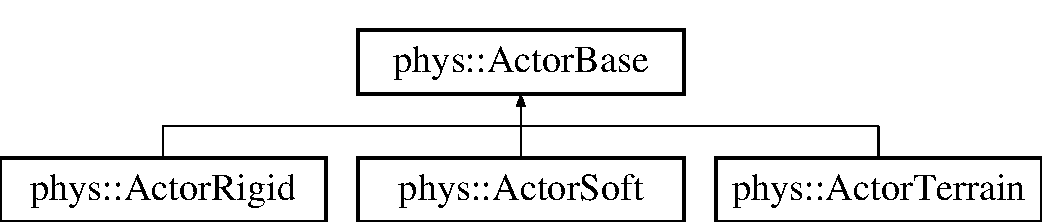
\includegraphics[height=2cm]{d8/d0f/classphys_1_1ActorBase}
\end{center}
\end{figure}
\subsection*{Public Member Functions}
\begin{DoxyCompactItemize}
\item 
virtual \hyperlink{classphys_1_1ActorBase_a5e5d4b50c83c6851e554b5e7ad65403f}{$\sim$ActorBase} ()
\begin{DoxyCompactList}\small\item\em Destructor. \item\end{DoxyCompactList}\item 
\hyperlink{classphys_1_1ActorBase_ad9d90a68921ce81653e9950c1330809d}{ActorBase} (\hyperlink{namespacephys_aa03900411993de7fbfec4789bc1d392e}{String} name, \hyperlink{namespacephys_aa03900411993de7fbfec4789bc1d392e}{String} file, \hyperlink{namespacephys_aa03900411993de7fbfec4789bc1d392e}{String} group, \hyperlink{classphys_1_1World}{World} $\ast$\_\-World)
\begin{DoxyCompactList}\small\item\em Descriptive constructor. \item\end{DoxyCompactList}\item 
void \hyperlink{classphys_1_1ActorBase_a0b0db2ec0f4926326635b86f1ead2276}{SetLocation} (\hyperlink{namespacephys_af7eb897198d265b8e868f45240230d5f}{Real} x, \hyperlink{namespacephys_af7eb897198d265b8e868f45240230d5f}{Real} y, \hyperlink{namespacephys_af7eb897198d265b8e868f45240230d5f}{Real} z)
\begin{DoxyCompactList}\small\item\em Manually sets the location of the actor. \item\end{DoxyCompactList}\item 
void \hyperlink{classphys_1_1ActorBase_a9a182b7262742ab5d499e7a51d407044}{SetLocation} (\hyperlink{classPhysVector3}{PhysVector3} Place)
\begin{DoxyCompactList}\small\item\em Manually sets the location of the actor. \item\end{DoxyCompactList}\item 
\hyperlink{classPhysVector3}{PhysVector3} \hyperlink{classphys_1_1ActorBase_ae402982d8c62acac7a122f24a289731d}{GetLocation} ()
\begin{DoxyCompactList}\small\item\em Retrieves the location of the object. \item\end{DoxyCompactList}\item 
void \hyperlink{classphys_1_1ActorBase_ab7513e8b650b40ea4387c170929457a7}{SetInitLocation} (\hyperlink{classPhysVector3}{PhysVector3} Location)
\begin{DoxyCompactList}\small\item\em Sets the starting location of the actor. \item\end{DoxyCompactList}\item 
void \hyperlink{classphys_1_1ActorBase_a681186465db767954ca3f9530a1d7c36}{SetInitOrientation} (\hyperlink{classphys_1_1Quaternion}{Quaternion} Orientation)
\begin{DoxyCompactList}\small\item\em Sets the starting orientation of the actor. \item\end{DoxyCompactList}\item 
void \hyperlink{classphys_1_1ActorBase_adbf0cc77031f22597a799fd0f7f8216d}{SetOrientation} (\hyperlink{namespacephys_af7eb897198d265b8e868f45240230d5f}{Real} x, \hyperlink{namespacephys_af7eb897198d265b8e868f45240230d5f}{Real} y, \hyperlink{namespacephys_af7eb897198d265b8e868f45240230d5f}{Real} z, \hyperlink{namespacephys_af7eb897198d265b8e868f45240230d5f}{Real} w)
\begin{DoxyCompactList}\small\item\em Sets the orientation of the actor. \item\end{DoxyCompactList}\item 
void \hyperlink{classphys_1_1ActorBase_ac4b0bf1eff730d94f72d04957efea69d}{SetOrientation} (\hyperlink{classphys_1_1Quaternion}{Quaternion} Rotation)
\begin{DoxyCompactList}\small\item\em Sets the orientation of the actor. \item\end{DoxyCompactList}\item 
void \hyperlink{classphys_1_1ActorBase_acd5613286ec14fb2a8e5ed5f5003dc5f}{SetKinematic} ()
\begin{DoxyCompactList}\small\item\em Sets the state of the object to Kinematic. \item\end{DoxyCompactList}\item 
void \hyperlink{classphys_1_1ActorBase_af0219532fe71d1d84042a20a88fe5037}{SetStatic} ()
\begin{DoxyCompactList}\small\item\em Sets the state of the object to Static. \item\end{DoxyCompactList}\end{DoxyCompactItemize}
\subsection*{Protected Member Functions}
\begin{DoxyCompactItemize}
\item 
virtual void \hyperlink{classphys_1_1ActorBase_ac5d4ad5a634b16000742f506ed5957fb}{AddObjectToWorld} (\hyperlink{classphys_1_1World}{World} $\ast$TargetWorld, btSoftRigidDynamicsWorld $\ast$btWorld)=0
\begin{DoxyCompactList}\small\item\em Adds the actor to the physics world. \item\end{DoxyCompactList}\item 
btTriangleMesh $\ast$ \hyperlink{classphys_1_1ActorBase_a4d2137276c50bbe5bc8cf9ecc66581b7}{CreateTrimesh} ()
\begin{DoxyCompactList}\small\item\em Creates a trimesh shape from the mesh file. \item\end{DoxyCompactList}\item 
void \hyperlink{classphys_1_1ActorBase_aff7dbb190fb982a43123bee3066501c4}{CreateEntity} (\hyperlink{namespacephys_aa03900411993de7fbfec4789bc1d392e}{String} name, \hyperlink{namespacephys_aa03900411993de7fbfec4789bc1d392e}{String} file, \hyperlink{namespacephys_aa03900411993de7fbfec4789bc1d392e}{String} group)
\begin{DoxyCompactList}\small\item\em Creates an entity for the mesh file to be placed on a scene node. \item\end{DoxyCompactList}\item 
void \hyperlink{classphys_1_1ActorBase_a125d6f0a0b4072e64490638c074eea2d}{CreateSceneNode} ()
\begin{DoxyCompactList}\small\item\em Creates a node for the entity in the graphical world. \item\end{DoxyCompactList}\item 
void \hyperlink{classphys_1_1ActorBase_af8a6cb524bda889b7a38f0245a7381fb}{SetOgreLocation} (\hyperlink{classPhysVector3}{PhysVector3} Place)
\begin{DoxyCompactList}\small\item\em Sets the location of the graphical body. \item\end{DoxyCompactList}\item 
\hyperlink{classPhysVector3}{PhysVector3} \hyperlink{classphys_1_1ActorBase_a52a65d23c76c805f4851191b62712ed8}{GetOgreLocation} ()
\begin{DoxyCompactList}\small\item\em Retrieves the location of the graphical body. \item\end{DoxyCompactList}\item 
void \hyperlink{classphys_1_1ActorBase_a7b2d13cb1e8bba60eeae782a53fd5e49}{SetOgreOrientation} (\hyperlink{classphys_1_1Quaternion}{Quaternion} Rotation)
\begin{DoxyCompactList}\small\item\em Sets the orientation of the graphical body. \item\end{DoxyCompactList}\item 
void \hyperlink{classphys_1_1ActorBase_a45f190cb9b647bb3385d1298f9dab589}{AttachToGraphics} ()
\begin{DoxyCompactList}\small\item\em Makes the actor visable. \item\end{DoxyCompactList}\item 
virtual void \hyperlink{classphys_1_1ActorBase_ab8d8c68937ea92b245b411c07b8bde7a}{SetBulletLocation} (\hyperlink{classPhysVector3}{PhysVector3} Location)
\begin{DoxyCompactList}\small\item\em Sets the location of the physics body. \item\end{DoxyCompactList}\item 
virtual \hyperlink{classPhysVector3}{PhysVector3} \hyperlink{classphys_1_1ActorBase_ac7c8bbb4859668d71325a791c88584ae}{GetBulletLocation} ()
\begin{DoxyCompactList}\small\item\em Retrieves the location of the physics body. \item\end{DoxyCompactList}\item 
virtual void \hyperlink{classphys_1_1ActorBase_a492244ac46ced53b809f436da992bc84}{SetBulletOrientation} (\hyperlink{classphys_1_1Quaternion}{Quaternion} Rotation)
\begin{DoxyCompactList}\small\item\em Sets the orientation of the physics body. \item\end{DoxyCompactList}\end{DoxyCompactItemize}
\subsection*{Protected Attributes}
\begin{DoxyCompactItemize}
\item 
\hypertarget{classphys_1_1ActorBase_a0ffbb74296ac96db26c890274df794a2}{
\hyperlink{classphys_1_1World}{World} $\ast$ \hyperlink{classphys_1_1ActorBase_a0ffbb74296ac96db26c890274df794a2}{GameWorld}}
\label{d8/d0f/classphys_1_1ActorBase_a0ffbb74296ac96db26c890274df794a2}

\begin{DoxyCompactList}\small\item\em A pointer to the \hyperlink{classphys_1_1World}{World} the actor will reside. \item\end{DoxyCompactList}\item 
\hypertarget{classphys_1_1ActorBase_ae44969ba242ca5c13a608b7467be0674}{
Ogre::Entity $\ast$ \hyperlink{classphys_1_1ActorBase_ae44969ba242ca5c13a608b7467be0674}{entity}}
\label{d8/d0f/classphys_1_1ActorBase_ae44969ba242ca5c13a608b7467be0674}

\begin{DoxyCompactList}\small\item\em This class encapsulates the functionality of the Ogre::Entity using this. \item\end{DoxyCompactList}\item 
\hypertarget{classphys_1_1ActorBase_a687bfa0cc44adf715651c7ac41a46321}{
Ogre::SceneNode $\ast$ \hyperlink{classphys_1_1ActorBase_a687bfa0cc44adf715651c7ac41a46321}{node}}
\label{d8/d0f/classphys_1_1ActorBase_a687bfa0cc44adf715651c7ac41a46321}

\begin{DoxyCompactList}\small\item\em This class encapsulates the functionality of the Ogre::SceneNode using this. \item\end{DoxyCompactList}\item 
\hypertarget{classphys_1_1ActorBase_a643613ce7abb4b6d4352bab036b7cf69}{
btCollisionShape $\ast$ \hyperlink{classphys_1_1ActorBase_a643613ce7abb4b6d4352bab036b7cf69}{Shape}}
\label{d8/d0f/classphys_1_1ActorBase_a643613ce7abb4b6d4352bab036b7cf69}

\begin{DoxyCompactList}\small\item\em This class encapsulates the functionality of the btCollisionShape using this. \item\end{DoxyCompactList}\item 
\hypertarget{classphys_1_1ActorBase_a70676c52ffee64705a7b463d29b60429}{
btCollisionObject $\ast$ \hyperlink{classphys_1_1ActorBase_a70676c52ffee64705a7b463d29b60429}{CollisionObject}}
\label{d8/d0f/classphys_1_1ActorBase_a70676c52ffee64705a7b463d29b60429}

\begin{DoxyCompactList}\small\item\em This class encapsulates the functionality of the btCollisionObject using this. \item\end{DoxyCompactList}\item 
\hypertarget{classphys_1_1ActorBase_a44934cb1db748c3c69e3b88a8dd17dcb}{
\hyperlink{classphys_1_1PhysMotionState}{PhysMotionState} $\ast$ \hyperlink{classphys_1_1ActorBase_a44934cb1db748c3c69e3b88a8dd17dcb}{MotionState}}
\label{d8/d0f/classphys_1_1ActorBase_a44934cb1db748c3c69e3b88a8dd17dcb}

\begin{DoxyCompactList}\small\item\em This class encapsulates the functionality of the \hyperlink{classphys_1_1PhysMotionState}{PhysMotionState} using this. \item\end{DoxyCompactList}\end{DoxyCompactItemize}
\subsection*{Friends}
\begin{DoxyCompactItemize}
\item 
\hypertarget{classphys_1_1ActorBase_ae18d4e9935739ce8709d2974a7e91b16}{
class \hyperlink{classphys_1_1ActorBase_ae18d4e9935739ce8709d2974a7e91b16}{phys::World}}
\label{d8/d0f/classphys_1_1ActorBase_ae18d4e9935739ce8709d2974a7e91b16}

\end{DoxyCompactItemize}


\subsection{Detailed Description}
This is the base class from which all the actors inherit. The actor classes store and manage all the relevant data regarding objects inside the \hyperlink{classphys_1_1World}{World}. They serve as a binder between the physics and graphics for objects and have functions that allow the manipulation of objects loaded into the \hyperlink{classphys_1_1World}{World}. Currently there are 4 actor classes: \hyperlink{classphys_1_1ActorBase}{ActorBase}, ActorDynRigid, ActorDynSoft, and ActorSta. \par
 \hyperlink{classphys_1_1ActorBase}{ActorBase} is a base class that serves as a template for the other three actor classes. \par
 \hyperlink{classphys_1_1ActorBase}{ActorBase} should never be created, as it lacks the functionality needed for most objects. 

Definition at line 92 of file physactor.h.



\subsection{Constructor \& Destructor Documentation}
\hypertarget{classphys_1_1ActorBase_a5e5d4b50c83c6851e554b5e7ad65403f}{
\index{phys::ActorBase@{phys::ActorBase}!$\sim$ActorBase@{$\sim$ActorBase}}
\index{$\sim$ActorBase@{$\sim$ActorBase}!phys::ActorBase@{phys::ActorBase}}
\subsubsection[{$\sim$ActorBase}]{\setlength{\rightskip}{0pt plus 5cm}phys::ActorBase::$\sim$ActorBase ()\hspace{0.3cm}{\ttfamily  \mbox{[}virtual\mbox{]}}}}
\label{d8/d0f/classphys_1_1ActorBase_a5e5d4b50c83c6851e554b5e7ad65403f}


Destructor. 

The class destructor. 

Definition at line 120 of file physactor.cpp.

\hypertarget{classphys_1_1ActorBase_ad9d90a68921ce81653e9950c1330809d}{
\index{phys::ActorBase@{phys::ActorBase}!ActorBase@{ActorBase}}
\index{ActorBase@{ActorBase}!phys::ActorBase@{phys::ActorBase}}
\subsubsection[{ActorBase}]{\setlength{\rightskip}{0pt plus 5cm}phys::ActorBase::ActorBase ({\bf String} {\em name}, \/  {\bf String} {\em file}, \/  {\bf String} {\em group}, \/  {\bf World} $\ast$ {\em \_\-World})}}
\label{d8/d0f/classphys_1_1ActorBase_ad9d90a68921ce81653e9950c1330809d}


Descriptive constructor. 

This constructor contains the basic information needed to make an actor. 
\begin{DoxyParams}{Parameters}
\item[{\em name}]The name of the actor. \item[{\em file}]The 3d mesh file that contains the 3d model the actor will use. \item[{\em group}]The resource group where the 3d mesh and other related files can be found. \item[{\em \_\-World}]Pointer to the \hyperlink{classphys_1_1World}{World} this object will be added to. \end{DoxyParams}


Definition at line 110 of file physactor.cpp.



\subsection{Member Function Documentation}
\hypertarget{classphys_1_1ActorBase_ac5d4ad5a634b16000742f506ed5957fb}{
\index{phys::ActorBase@{phys::ActorBase}!AddObjectToWorld@{AddObjectToWorld}}
\index{AddObjectToWorld@{AddObjectToWorld}!phys::ActorBase@{phys::ActorBase}}
\subsubsection[{AddObjectToWorld}]{\setlength{\rightskip}{0pt plus 5cm}virtual void phys::ActorBase::AddObjectToWorld ({\bf World} $\ast$ {\em TargetWorld}, \/  btSoftRigidDynamicsWorld $\ast$ {\em btWorld})\hspace{0.3cm}{\ttfamily  \mbox{[}protected, pure virtual\mbox{]}}}}
\label{d8/d0f/classphys_1_1ActorBase_ac5d4ad5a634b16000742f506ed5957fb}


Adds the actor to the physics world. 

Adds the actor to the physics world. \par
 This is automaticly called by the PhysWorlds AddActor function and shouldn't be called manually. 
\begin{DoxyParams}{Parameters}
\item[{\em TargetWorld}]Pointer to the \hyperlink{classphys_1_1World}{World} class. \item[{\em btWorld}]Pointer to the physics world. \end{DoxyParams}


Implemented in \hyperlink{classphys_1_1ActorRigid_a3c56eb06fe6a7d468b7a67c45ade7be4}{phys::ActorRigid}, and \hyperlink{classphys_1_1ActorSoft_a3a704ab32f847a5d0e060f8a592efefd}{phys::ActorSoft}.

\hypertarget{classphys_1_1ActorBase_a45f190cb9b647bb3385d1298f9dab589}{
\index{phys::ActorBase@{phys::ActorBase}!AttachToGraphics@{AttachToGraphics}}
\index{AttachToGraphics@{AttachToGraphics}!phys::ActorBase@{phys::ActorBase}}
\subsubsection[{AttachToGraphics}]{\setlength{\rightskip}{0pt plus 5cm}void phys::ActorBase::AttachToGraphics ()\hspace{0.3cm}{\ttfamily  \mbox{[}protected\mbox{]}}}}
\label{d8/d0f/classphys_1_1ActorBase_a45f190cb9b647bb3385d1298f9dab589}


Makes the actor visable. 

Adds the actor to all the nessessary graphics elements to make it visable on screen. \par
 This is automaticly called by the PhysWorlds AddActor function and shouldn't ever need to be called manually. 

Definition at line 321 of file physactor.cpp.

\hypertarget{classphys_1_1ActorBase_aff7dbb190fb982a43123bee3066501c4}{
\index{phys::ActorBase@{phys::ActorBase}!CreateEntity@{CreateEntity}}
\index{CreateEntity@{CreateEntity}!phys::ActorBase@{phys::ActorBase}}
\subsubsection[{CreateEntity}]{\setlength{\rightskip}{0pt plus 5cm}void phys::ActorBase::CreateEntity ({\bf String} {\em name}, \/  {\bf String} {\em file}, \/  {\bf String} {\em group})\hspace{0.3cm}{\ttfamily  \mbox{[}protected\mbox{]}}}}
\label{d8/d0f/classphys_1_1ActorBase_aff7dbb190fb982a43123bee3066501c4}


Creates an entity for the mesh file to be placed on a scene node. 

Creates an entity in the scene manager from the mesh file provided to be attached to a node in the graphical world. \par
 This function is called on by the Constructor, and shouldn't be called manually. 
\begin{DoxyParams}{Parameters}
\item[{\em name}]Name of the actor. \item[{\em file}]File name of the graphical mesh to be used. \item[{\em group}]Resource group where the graphical mesh can be found. \end{DoxyParams}


Definition at line 220 of file physactor.cpp.

\hypertarget{classphys_1_1ActorBase_a125d6f0a0b4072e64490638c074eea2d}{
\index{phys::ActorBase@{phys::ActorBase}!CreateSceneNode@{CreateSceneNode}}
\index{CreateSceneNode@{CreateSceneNode}!phys::ActorBase@{phys::ActorBase}}
\subsubsection[{CreateSceneNode}]{\setlength{\rightskip}{0pt plus 5cm}void phys::ActorBase::CreateSceneNode ()\hspace{0.3cm}{\ttfamily  \mbox{[}protected\mbox{]}}}}
\label{d8/d0f/classphys_1_1ActorBase_a125d6f0a0b4072e64490638c074eea2d}


Creates a node for the entity in the graphical world. 

Creates a node in the scene manager to attach the actor's entity to within the graphical world. \par
 This function is called on by the Constructor, and shouldn't be called manually. 

Definition at line 225 of file physactor.cpp.

\hypertarget{classphys_1_1ActorBase_a4d2137276c50bbe5bc8cf9ecc66581b7}{
\index{phys::ActorBase@{phys::ActorBase}!CreateTrimesh@{CreateTrimesh}}
\index{CreateTrimesh@{CreateTrimesh}!phys::ActorBase@{phys::ActorBase}}
\subsubsection[{CreateTrimesh}]{\setlength{\rightskip}{0pt plus 5cm}btTriangleMesh $\ast$ phys::ActorBase::CreateTrimesh ()\hspace{0.3cm}{\ttfamily  \mbox{[}protected\mbox{]}}}}
\label{d8/d0f/classphys_1_1ActorBase_a4d2137276c50bbe5bc8cf9ecc66581b7}


Creates a trimesh shape from the mesh file. 

Makes a trimesh to be used as a collision shape in the physics world from a mesh file. \par
 This is automaticly called by the CreateShapeFromMesh function in child classes and shouldn't be called manually. 

Definition at line 129 of file physactor.cpp.

\hypertarget{classphys_1_1ActorBase_ac7c8bbb4859668d71325a791c88584ae}{
\index{phys::ActorBase@{phys::ActorBase}!GetBulletLocation@{GetBulletLocation}}
\index{GetBulletLocation@{GetBulletLocation}!phys::ActorBase@{phys::ActorBase}}
\subsubsection[{GetBulletLocation}]{\setlength{\rightskip}{0pt plus 5cm}{\bf PhysVector3} phys::ActorBase::GetBulletLocation ()\hspace{0.3cm}{\ttfamily  \mbox{[}protected, virtual\mbox{]}}}}
\label{d8/d0f/classphys_1_1ActorBase_ac7c8bbb4859668d71325a791c88584ae}


Retrieves the location of the physics body. 

This function will retrieve the location of the object within the physics world. 

Definition at line 251 of file physactor.cpp.

\hypertarget{classphys_1_1ActorBase_ae402982d8c62acac7a122f24a289731d}{
\index{phys::ActorBase@{phys::ActorBase}!GetLocation@{GetLocation}}
\index{GetLocation@{GetLocation}!phys::ActorBase@{phys::ActorBase}}
\subsubsection[{GetLocation}]{\setlength{\rightskip}{0pt plus 5cm}{\bf PhysVector3} phys::ActorBase::GetLocation ()}}
\label{d8/d0f/classphys_1_1ActorBase_ae402982d8c62acac7a122f24a289731d}


Retrieves the location of the object. 

This function will retrieve the location of the object within the world. 

Definition at line 288 of file physactor.cpp.

\hypertarget{classphys_1_1ActorBase_a52a65d23c76c805f4851191b62712ed8}{
\index{phys::ActorBase@{phys::ActorBase}!GetOgreLocation@{GetOgreLocation}}
\index{GetOgreLocation@{GetOgreLocation}!phys::ActorBase@{phys::ActorBase}}
\subsubsection[{GetOgreLocation}]{\setlength{\rightskip}{0pt plus 5cm}{\bf PhysVector3} phys::ActorBase::GetOgreLocation ()\hspace{0.3cm}{\ttfamily  \mbox{[}protected\mbox{]}}}}
\label{d8/d0f/classphys_1_1ActorBase_a52a65d23c76c805f4851191b62712ed8}


Retrieves the location of the graphical body. 

This function will retrieve the location of the object within the graphical world. 

Definition at line 238 of file physactor.cpp.

\hypertarget{classphys_1_1ActorBase_ab8d8c68937ea92b245b411c07b8bde7a}{
\index{phys::ActorBase@{phys::ActorBase}!SetBulletLocation@{SetBulletLocation}}
\index{SetBulletLocation@{SetBulletLocation}!phys::ActorBase@{phys::ActorBase}}
\subsubsection[{SetBulletLocation}]{\setlength{\rightskip}{0pt plus 5cm}void phys::ActorBase::SetBulletLocation ({\bf PhysVector3} {\em Location})\hspace{0.3cm}{\ttfamily  \mbox{[}protected, virtual\mbox{]}}}}
\label{d8/d0f/classphys_1_1ActorBase_ab8d8c68937ea92b245b411c07b8bde7a}


Sets the location of the physics body. 

This will take a \hyperlink{classPhysVector3}{PhysVector3} and set the location of the actor within the physics world. \par
 This function is called on by the SetLocation function, and shouldn't be called manually. 
\begin{DoxyParams}{Parameters}
\item[{\em Location}]The \hyperlink{classPhysVector3}{PhysVector3} representing the location. \end{DoxyParams}


Definition at line 245 of file physactor.cpp.

\hypertarget{classphys_1_1ActorBase_a492244ac46ced53b809f436da992bc84}{
\index{phys::ActorBase@{phys::ActorBase}!SetBulletOrientation@{SetBulletOrientation}}
\index{SetBulletOrientation@{SetBulletOrientation}!phys::ActorBase@{phys::ActorBase}}
\subsubsection[{SetBulletOrientation}]{\setlength{\rightskip}{0pt plus 5cm}void phys::ActorBase::SetBulletOrientation ({\bf Quaternion} {\em Rotation})\hspace{0.3cm}{\ttfamily  \mbox{[}protected, virtual\mbox{]}}}}
\label{d8/d0f/classphys_1_1ActorBase_a492244ac46ced53b809f436da992bc84}


Sets the orientation of the physics body. 

This will take a PhysQuaternion and set the orientation of the actor within the physics world. \par
 This function is called on by the SetOrientation function, and shouldn't be called manually. 
\begin{DoxyParams}{Parameters}
\item[{\em Rotation}]The quaternion representing the rotation of the actor. \end{DoxyParams}


Definition at line 267 of file physactor.cpp.

\hypertarget{classphys_1_1ActorBase_ab7513e8b650b40ea4387c170929457a7}{
\index{phys::ActorBase@{phys::ActorBase}!SetInitLocation@{SetInitLocation}}
\index{SetInitLocation@{SetInitLocation}!phys::ActorBase@{phys::ActorBase}}
\subsubsection[{SetInitLocation}]{\setlength{\rightskip}{0pt plus 5cm}void phys::ActorBase::SetInitLocation ({\bf PhysVector3} {\em Location})}}
\label{d8/d0f/classphys_1_1ActorBase_ab7513e8b650b40ea4387c170929457a7}


Sets the starting location of the actor. 

Calling this function after adding it to the \hyperlink{classphys_1_1World}{World} will have no effect. \par
 This function will set where the actor will be located in the \hyperlink{classphys_1_1World}{World} when it is first placed inside the world. 
\begin{DoxyParams}{Parameters}
\item[{\em Location}]The \hyperlink{classPhysVector3}{PhysVector3} representing the location. \end{DoxyParams}


Definition at line 293 of file physactor.cpp.

\hypertarget{classphys_1_1ActorBase_a681186465db767954ca3f9530a1d7c36}{
\index{phys::ActorBase@{phys::ActorBase}!SetInitOrientation@{SetInitOrientation}}
\index{SetInitOrientation@{SetInitOrientation}!phys::ActorBase@{phys::ActorBase}}
\subsubsection[{SetInitOrientation}]{\setlength{\rightskip}{0pt plus 5cm}void phys::ActorBase::SetInitOrientation ({\bf Quaternion} {\em Orientation})}}
\label{d8/d0f/classphys_1_1ActorBase_a681186465db767954ca3f9530a1d7c36}


Sets the starting orientation of the actor. 

Calling this function after adding it to the \hyperlink{classphys_1_1World}{World} will have no effect. \par
 This function will set where the actor is facing in the \hyperlink{classphys_1_1World}{World} when it is first placed inside the world. 
\begin{DoxyParams}{Parameters}
\item[{\em Orientation}]The PhysQuaternion representing the Orientation. \end{DoxyParams}


Definition at line 301 of file physactor.cpp.

\hypertarget{classphys_1_1ActorBase_acd5613286ec14fb2a8e5ed5f5003dc5f}{
\index{phys::ActorBase@{phys::ActorBase}!SetKinematic@{SetKinematic}}
\index{SetKinematic@{SetKinematic}!phys::ActorBase@{phys::ActorBase}}
\subsubsection[{SetKinematic}]{\setlength{\rightskip}{0pt plus 5cm}void phys::ActorBase::SetKinematic ()}}
\label{d8/d0f/classphys_1_1ActorBase_acd5613286ec14fb2a8e5ed5f5003dc5f}


Sets the state of the object to Kinematic. 

This function will set the object to a Kinematic Object. \par
 Kinematic Objects are like Static Objects but are also able to be moved directly by character controllers. 

Definition at line 333 of file physactor.cpp.

\hypertarget{classphys_1_1ActorBase_a9a182b7262742ab5d499e7a51d407044}{
\index{phys::ActorBase@{phys::ActorBase}!SetLocation@{SetLocation}}
\index{SetLocation@{SetLocation}!phys::ActorBase@{phys::ActorBase}}
\subsubsection[{SetLocation}]{\setlength{\rightskip}{0pt plus 5cm}void phys::ActorBase::SetLocation ({\bf PhysVector3} {\em Place})}}
\label{d8/d0f/classphys_1_1ActorBase_a9a182b7262742ab5d499e7a51d407044}


Manually sets the location of the actor. 

Calling this function prior to adding it to the \hyperlink{classphys_1_1World}{World} will have no effect. \par
 In most situations you won't want to use this function, and instead produce movement through physics functions. 
\begin{DoxyParams}{Parameters}
\item[{\em Place}]The \hyperlink{classPhysVector3}{PhysVector3} representing the location. \end{DoxyParams}


Definition at line 282 of file physactor.cpp.

\hypertarget{classphys_1_1ActorBase_a0b0db2ec0f4926326635b86f1ead2276}{
\index{phys::ActorBase@{phys::ActorBase}!SetLocation@{SetLocation}}
\index{SetLocation@{SetLocation}!phys::ActorBase@{phys::ActorBase}}
\subsubsection[{SetLocation}]{\setlength{\rightskip}{0pt plus 5cm}void phys::ActorBase::SetLocation ({\bf Real} {\em x}, \/  {\bf Real} {\em y}, \/  {\bf Real} {\em z})}}
\label{d8/d0f/classphys_1_1ActorBase_a0b0db2ec0f4926326635b86f1ead2276}


Manually sets the location of the actor. 

Calling this function prior to adding it to the \hyperlink{classphys_1_1World}{World} will have no effect. \par
 In most situations you won't want to use this function, and instead produce movement through physics functions. 
\begin{DoxyParams}{Parameters}
\item[{\em x}]Location on the X vector. \item[{\em y}]Location on the Y vector. \item[{\em z}]Location on the Z vector. \end{DoxyParams}


Definition at line 276 of file physactor.cpp.

\hypertarget{classphys_1_1ActorBase_af8a6cb524bda889b7a38f0245a7381fb}{
\index{phys::ActorBase@{phys::ActorBase}!SetOgreLocation@{SetOgreLocation}}
\index{SetOgreLocation@{SetOgreLocation}!phys::ActorBase@{phys::ActorBase}}
\subsubsection[{SetOgreLocation}]{\setlength{\rightskip}{0pt plus 5cm}void phys::ActorBase::SetOgreLocation ({\bf PhysVector3} {\em Place})\hspace{0.3cm}{\ttfamily  \mbox{[}protected\mbox{]}}}}
\label{d8/d0f/classphys_1_1ActorBase_af8a6cb524bda889b7a38f0245a7381fb}


Sets the location of the graphical body. 

This will take a \hyperlink{classPhysVector3}{PhysVector3} and set the location of the actor within the graphical world. \par
 This function is called on by the SetLocation function, and shouldn't be called manually. 
\begin{DoxyParams}{Parameters}
\item[{\em Place}]The \hyperlink{classPhysVector3}{PhysVector3} representing the location. \end{DoxyParams}


Definition at line 233 of file physactor.cpp.

\hypertarget{classphys_1_1ActorBase_a7b2d13cb1e8bba60eeae782a53fd5e49}{
\index{phys::ActorBase@{phys::ActorBase}!SetOgreOrientation@{SetOgreOrientation}}
\index{SetOgreOrientation@{SetOgreOrientation}!phys::ActorBase@{phys::ActorBase}}
\subsubsection[{SetOgreOrientation}]{\setlength{\rightskip}{0pt plus 5cm}void phys::ActorBase::SetOgreOrientation ({\bf Quaternion} {\em Rotation})\hspace{0.3cm}{\ttfamily  \mbox{[}protected\mbox{]}}}}
\label{d8/d0f/classphys_1_1ActorBase_a7b2d13cb1e8bba60eeae782a53fd5e49}


Sets the orientation of the graphical body. 

This will take a PhysQuaternion and set the orientation of the actor within the graphical world. \par
 This function is called on by the SetOrientation function, and shouldn't be called manually. 
\begin{DoxyParams}{Parameters}
\item[{\em Rotation}]The quaternion representing the rotation of the actor. \end{DoxyParams}


Definition at line 262 of file physactor.cpp.

\hypertarget{classphys_1_1ActorBase_ac4b0bf1eff730d94f72d04957efea69d}{
\index{phys::ActorBase@{phys::ActorBase}!SetOrientation@{SetOrientation}}
\index{SetOrientation@{SetOrientation}!phys::ActorBase@{phys::ActorBase}}
\subsubsection[{SetOrientation}]{\setlength{\rightskip}{0pt plus 5cm}void phys::ActorBase::SetOrientation ({\bf Quaternion} {\em Rotation})}}
\label{d8/d0f/classphys_1_1ActorBase_ac4b0bf1eff730d94f72d04957efea69d}


Sets the orientation of the actor. 

Sets the orientation of the actor via a \hyperlink{classphys_1_1Quaternion}{Quaternion}. 
\begin{DoxyParams}{Parameters}
\item[{\em Rotation}]The \hyperlink{classphys_1_1Quaternion}{Quaternion} representing the Rotation. \end{DoxyParams}


Definition at line 312 of file physactor.cpp.

\hypertarget{classphys_1_1ActorBase_adbf0cc77031f22597a799fd0f7f8216d}{
\index{phys::ActorBase@{phys::ActorBase}!SetOrientation@{SetOrientation}}
\index{SetOrientation@{SetOrientation}!phys::ActorBase@{phys::ActorBase}}
\subsubsection[{SetOrientation}]{\setlength{\rightskip}{0pt plus 5cm}void phys::ActorBase::SetOrientation ({\bf Real} {\em x}, \/  {\bf Real} {\em y}, \/  {\bf Real} {\em z}, \/  {\bf Real} {\em w})}}
\label{d8/d0f/classphys_1_1ActorBase_adbf0cc77031f22597a799fd0f7f8216d}


Sets the orientation of the actor. 

Sets the orientation of the actor via \hyperlink{classphys_1_1Quaternion}{Quaternion} parameters. 
\begin{DoxyParams}{Parameters}
\item[{\em x}]Where the X vector is rotated about. \item[{\em y}]Where the Y vector is rotated about. \item[{\em z}]Where the Z vector is rotated about. \item[{\em w}]How much to about the x, y, z. \end{DoxyParams}


Definition at line 306 of file physactor.cpp.

\hypertarget{classphys_1_1ActorBase_af0219532fe71d1d84042a20a88fe5037}{
\index{phys::ActorBase@{phys::ActorBase}!SetStatic@{SetStatic}}
\index{SetStatic@{SetStatic}!phys::ActorBase@{phys::ActorBase}}
\subsubsection[{SetStatic}]{\setlength{\rightskip}{0pt plus 5cm}void phys::ActorBase::SetStatic ()}}
\label{d8/d0f/classphys_1_1ActorBase_af0219532fe71d1d84042a20a88fe5037}


Sets the state of the object to Static. 

This function will set the object to a Static Object. \par
 Static Objects don't move or have any force applied to them, but are cabable of exerting force on other objects. 

Definition at line 339 of file physactor.cpp.



The documentation for this class was generated from the following files:\begin{DoxyCompactItemize}
\item 
physactor.h\item 
physactor.cpp\end{DoxyCompactItemize}

\hypertarget{classphys_1_1ActorContainerBase}{
\subsection{phys::ActorContainerBase Class Reference}
\label{classphys_1_1ActorContainerBase}\index{phys::ActorContainerBase@{phys::ActorContainerBase}}
}


A base class to unify the interface for different kinds of containers for holding actors.  




{\ttfamily \#include $<$actorcontainerbase.h$>$}

Inheritance diagram for phys::ActorContainerBase:\begin{figure}[H]
\begin{center}
\leavevmode
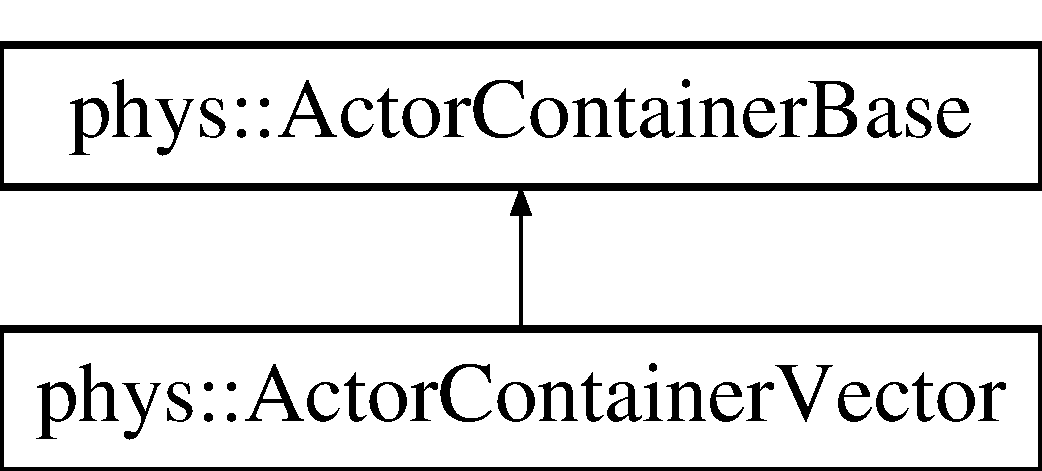
\includegraphics[height=2.000000cm]{classphys_1_1ActorContainerBase}
\end{center}
\end{figure}
\subsubsection*{Public Member Functions}
\begin{DoxyCompactItemize}
\item 
\hyperlink{classphys_1_1ActorContainerBase_ac17a442ad8aacba14d1cef956c0ddbb8}{ActorContainerBase} ()
\begin{DoxyCompactList}\small\item\em Basic Constructor. \item\end{DoxyCompactList}\item 
virtual \hyperlink{classphys_1_1ActorContainerBase_aa5eac062dd70a220a4ec6df973c6f258}{$\sim$ActorContainerBase} ()
\begin{DoxyCompactList}\small\item\em Destructor. \item\end{DoxyCompactList}\item 
virtual void \hyperlink{classphys_1_1ActorContainerBase_a8dd213cba4915f68ac421fc9f341cbbe}{AddActor} (\hyperlink{classphys_1_1ActorBase}{ActorBase} $\ast$ActorToAdd)=0
\begin{DoxyCompactList}\small\item\em This will add an Actor to this container and the world. \item\end{DoxyCompactList}\item 
virtual \hyperlink{classphys_1_1ActorBase}{ActorBase} $\ast$ \hyperlink{classphys_1_1ActorContainerBase_a6ccc6d058bcbbe0b9a638e28fb136477}{LastActorAdded} ()=0
\begin{DoxyCompactList}\small\item\em This provides an easy way to access the last Actor added to this container. \item\end{DoxyCompactList}\item 
virtual void \hyperlink{classphys_1_1ActorContainerBase_a523072e42f6b581d044432f84a84ede4}{RemoveActor} (\hyperlink{classphys_1_1ActorBase}{ActorBase} $\ast$ActorToRemove)=0
\begin{DoxyCompactList}\small\item\em Remove an Actor. \item\end{DoxyCompactList}\item 
virtual void \hyperlink{classphys_1_1ActorContainerBase_a60f37a056e8750f3b389c5ceed14520c}{RemoveActorAtCursor} ()=0
\begin{DoxyCompactList}\small\item\em Removes the current actor. \item\end{DoxyCompactList}\item 
\hypertarget{classphys_1_1ActorContainerBase_abc75d53e24ca0d9c2d9dcd14f6107149}{
virtual void \hyperlink{classphys_1_1ActorContainerBase_abc75d53e24ca0d9c2d9dcd14f6107149}{RemoveAllActors} ()=0}
\label{classphys_1_1ActorContainerBase_abc75d53e24ca0d9c2d9dcd14f6107149}

\begin{DoxyCompactList}\small\item\em Clears this container of all actors it is storing. \item\end{DoxyCompactList}\item 
virtual \hyperlink{namespacephys_a460f6bc24c8dd347b05e0366ae34f34a}{Whole} \hyperlink{classphys_1_1ActorContainerBase_aa5ec651d4634b2d90efe2a76f9d2fbdd}{GetActorCount} () const =0
\begin{DoxyCompactList}\small\item\em Returns how many actors this stores. \item\end{DoxyCompactList}\item 
virtual void \hyperlink{classphys_1_1ActorContainerBase_ab1a44758d7c17e70ff2e0f8de47424c3}{CursorToFirst} ()=0
\begin{DoxyCompactList}\small\item\em This moves the cursor to the first item in the container. \item\end{DoxyCompactList}\item 
virtual void \hyperlink{classphys_1_1ActorContainerBase_a7c424168c0bbd973b283a083714123b3}{CursorToPrevious} ()=0
\begin{DoxyCompactList}\small\item\em This moves the cursor to the previous item in the container. \item\end{DoxyCompactList}\item 
virtual void \hyperlink{classphys_1_1ActorContainerBase_a1aa337456a4e74cb5740dbae08778072}{CursorToNext} ()=0
\begin{DoxyCompactList}\small\item\em This moves the cursor to the next item in the container. \item\end{DoxyCompactList}\item 
virtual void \hyperlink{classphys_1_1ActorContainerBase_afad072e018a04c190e5e5fb93b82b354}{CursorToLast} ()=0
\begin{DoxyCompactList}\small\item\em This moves the cursor to the last item in the container. \item\end{DoxyCompactList}\item 
virtual \hyperlink{classphys_1_1ActorBase}{ActorBase} $\ast$ \hyperlink{classphys_1_1ActorContainerBase_a2c8fb86a9e188aece105b2a753ccc19a}{GetAtCursor} () const =0
\begin{DoxyCompactList}\small\item\em This gets the actor at the cursor. \item\end{DoxyCompactList}\item 
virtual \hyperlink{classphys_1_1ActorBase}{ActorBase} $\ast$ \hyperlink{classphys_1_1ActorContainerBase_ae703482d84a9c6726e28a8f26418b161}{GetFirst} () const =0
\begin{DoxyCompactList}\small\item\em This gets the first actor in the container. \item\end{DoxyCompactList}\item 
virtual \hyperlink{classphys_1_1ActorBase}{ActorBase} $\ast$ \hyperlink{classphys_1_1ActorContainerBase_a8efeffd5ae22085fe01af791b3ea559e}{GetLast} () const =0
\begin{DoxyCompactList}\small\item\em This gets the last actor in the container. \item\end{DoxyCompactList}\item 
virtual \hyperlink{classphys_1_1ActorBase}{ActorBase} $\ast$ \hyperlink{classphys_1_1ActorContainerBase_a1ade0001858f87ce1843cc6f6ec4e1c0}{FindActor} (Ogre::SceneNode $\ast$GraphicsNode)=0
\begin{DoxyCompactList}\small\item\em This finds an actor by searching for a graphics subsystem nodes. \item\end{DoxyCompactList}\item 
virtual \hyperlink{classphys_1_1ActorBase}{ActorBase} $\ast$ \hyperlink{classphys_1_1ActorContainerBase_a9ba6e38e0f12ada968cfee72fe5144d4}{FindActor} (btCollisionObject $\ast$PhysicsObject)=0
\begin{DoxyCompactList}\small\item\em This finds an actor by searching for a physics subsystem object. \item\end{DoxyCompactList}\item 
virtual \hyperlink{classphys_1_1ActorBase}{ActorBase} $\ast$ \hyperlink{classphys_1_1ActorContainerBase_a91223cbaebb8e5f11a4f971d7e5b64b6}{FindActor} (\hyperlink{namespacephys_aa03900411993de7fbfec4789bc1d392e}{String} Name)=0
\begin{DoxyCompactList}\small\item\em This finds an actor based on its name. \item\end{DoxyCompactList}\item 
virtual \hyperlink{namespacephys_aa03900411993de7fbfec4789bc1d392e}{String} \hyperlink{classphys_1_1ActorContainerBase_a0ed43bc828aaee8ee33152970c3cc16d}{GetContainerType} () const =0
\begin{DoxyCompactList}\small\item\em Which kind of container it this anyway. \item\end{DoxyCompactList}\item 
virtual \hyperlink{classphys_1_1World}{World} $\ast$ \hyperlink{classphys_1_1ActorContainerBase_a479e6c7434f2611b0cfe6ca1fd4ebdd1}{GetGameWorld} () const =0
\begin{DoxyCompactList}\small\item\em This gets the \hyperlink{classphys_1_1World}{World} that this class is working with. \item\end{DoxyCompactList}\item 
virtual void \hyperlink{classphys_1_1ActorContainerBase_ae0cb5c288f17507247dd98d3a2466876}{SetGameWorld} (\hyperlink{classphys_1_1World}{World} $\ast$GameWorld\_\-)=0
\begin{DoxyCompactList}\small\item\em This sets the \hyperlink{classphys_1_1World}{phys::World} that this Manager works with. \item\end{DoxyCompactList}\item 
virtual void \hyperlink{classphys_1_1ActorContainerBase_a366c1797bef08f3a1846bf010e2e2b04}{SetGameWorld} (\hyperlink{classphys_1_1World}{World} $\ast$GameWorld\_\-, bool AddToWorld, bool RemoveFromWorld)=0
\begin{DoxyCompactList}\small\item\em Optionally move actors into or out of a physworld. \item\end{DoxyCompactList}\end{DoxyCompactItemize}
\subsubsection*{Protected Member Functions}
\begin{DoxyCompactItemize}
\item 
\hypertarget{classphys_1_1ActorContainerBase_a44adf1174e624d9fa1408c9885f9ea12}{
Ogre::SceneNode $\ast$ \hyperlink{classphys_1_1ActorContainerBase_a44adf1174e624d9fa1408c9885f9ea12}{GetNode} (\hyperlink{classphys_1_1ActorBase}{ActorBase} $\ast$actor) const }
\label{classphys_1_1ActorContainerBase_a44adf1174e624d9fa1408c9885f9ea12}

\begin{DoxyCompactList}\small\item\em Used to work around the scenenode of an Actor being private, so all derived Containers can access it. \item\end{DoxyCompactList}\item 
\hypertarget{classphys_1_1ActorContainerBase_a3f3d84f7775d2e8597290e214fedd5f9}{
btCollisionObject $\ast$ \hyperlink{classphys_1_1ActorContainerBase_a3f3d84f7775d2e8597290e214fedd5f9}{GetCollisionObject} (\hyperlink{classphys_1_1ActorBase}{ActorBase} $\ast$actor) const }
\label{classphys_1_1ActorContainerBase_a3f3d84f7775d2e8597290e214fedd5f9}

\begin{DoxyCompactList}\small\item\em Used to work around the collision object of an Actor being private, so all derived Containers can access it. \item\end{DoxyCompactList}\end{DoxyCompactItemize}


\subsubsection{Detailed Description}
A base class to unify the interface for different kinds of containers for holding actors. Containers for actors must implement atleast this interface(abstract base class) to be usable with the \hyperlink{classphys_1_1World}{phys::World} for tracking in game objects. There are several reasons why this will be useful. Our first thought was deriving from this and an STL container like vector or list. Members of this class should be implementing or inheriting a proper container\par
\par
 The phys world will use one of these containers to store all of the actors for tracking purposes Since \par
\par
 In theory you should be be able to work with multiple actor containers and swiftly add or remove them to ad from a world to quickly control what actors are being worked with. It should even be possible to remove all actors, or have multiple set of actor in the world if you use the GameWorldSet methods carefully. \par
\par
 Additionally the is no reason an actor could be in multiple containers so this can provide even more options for actor sorting and categorization at runtime. \par
\par
 Because of this classes representation of a cursor only 1 thread at a time should use the cursor movement functions. For the container that the \hyperlink{classphys_1_1World}{phys::World} keeps it should be assume that the cursor is used. For other containers you should manage you container carefully and/or use another iteration method, such as STL iterators. 

Definition at line 76 of file actorcontainerbase.h.



\subsubsection{Constructor \& Destructor Documentation}
\hypertarget{classphys_1_1ActorContainerBase_ac17a442ad8aacba14d1cef956c0ddbb8}{
\index{phys::ActorContainerBase@{phys::ActorContainerBase}!ActorContainerBase@{ActorContainerBase}}
\index{ActorContainerBase@{ActorContainerBase}!phys::ActorContainerBase@{phys::ActorContainerBase}}
\paragraph[{ActorContainerBase}]{\setlength{\rightskip}{0pt plus 5cm}phys::ActorContainerBase::ActorContainerBase (
\begin{DoxyParamCaption}
{}
\end{DoxyParamCaption}
)}\hfill}
\label{classphys_1_1ActorContainerBase_ac17a442ad8aacba14d1cef956c0ddbb8}


Basic Constructor. 

This just assigned the passed pointer to ParentWorld 

Definition at line 54 of file actorcontainerbase.cpp.

\hypertarget{classphys_1_1ActorContainerBase_aa5eac062dd70a220a4ec6df973c6f258}{
\index{phys::ActorContainerBase@{phys::ActorContainerBase}!$\sim$ActorContainerBase@{$\sim$ActorContainerBase}}
\index{$\sim$ActorContainerBase@{$\sim$ActorContainerBase}!phys::ActorContainerBase@{phys::ActorContainerBase}}
\paragraph[{$\sim$ActorContainerBase}]{\setlength{\rightskip}{0pt plus 5cm}phys::ActorContainerBase::$\sim$ActorContainerBase (
\begin{DoxyParamCaption}
{}
\end{DoxyParamCaption}
)\hspace{0.3cm}{\ttfamily  \mbox{[}virtual\mbox{]}}}\hfill}
\label{classphys_1_1ActorContainerBase_aa5eac062dd70a220a4ec6df973c6f258}


Destructor. 

This really doesn't do anything, but if someone needs to overload it, it's here 

Definition at line 57 of file actorcontainerbase.cpp.



\subsubsection{Member Function Documentation}
\hypertarget{classphys_1_1ActorContainerBase_a8dd213cba4915f68ac421fc9f341cbbe}{
\index{phys::ActorContainerBase@{phys::ActorContainerBase}!AddActor@{AddActor}}
\index{AddActor@{AddActor}!phys::ActorContainerBase@{phys::ActorContainerBase}}
\paragraph[{AddActor}]{\setlength{\rightskip}{0pt plus 5cm}virtual void phys::ActorContainerBase::AddActor (
\begin{DoxyParamCaption}
\item[{{\bf ActorBase} $\ast$}]{ActorToAdd}
\end{DoxyParamCaption}
)\hspace{0.3cm}{\ttfamily  \mbox{[}pure virtual\mbox{]}}}\hfill}
\label{classphys_1_1ActorContainerBase_a8dd213cba4915f68ac421fc9f341cbbe}


This will add an Actor to this container and the world. 

This will add an Actor to this container and the world, and handle the nitty gritty details of add this to physics subsystem and graphics subsystem. \par
\par
 This will not add the Actor to any specific location in the ordering of the container. \par
\par
 It is expected that any container implementing this method will take appropriate steps to insure That the actor involved is added to the Physics and graphics world. This method could be called from derived to accomplish that task 
\begin{DoxyParams}{Parameters}
{\em ActorToAdd} & This is a pointer to the actor to add. \\
\hline
\end{DoxyParams}


Implemented in \hyperlink{classphys_1_1ActorContainerVector_a4bc3e38f16caddee021a97739bebaf6e}{phys::ActorContainerVector}.

\hypertarget{classphys_1_1ActorContainerBase_ab1a44758d7c17e70ff2e0f8de47424c3}{
\index{phys::ActorContainerBase@{phys::ActorContainerBase}!CursorToFirst@{CursorToFirst}}
\index{CursorToFirst@{CursorToFirst}!phys::ActorContainerBase@{phys::ActorContainerBase}}
\paragraph[{CursorToFirst}]{\setlength{\rightskip}{0pt plus 5cm}virtual void phys::ActorContainerBase::CursorToFirst (
\begin{DoxyParamCaption}
{}
\end{DoxyParamCaption}
)\hspace{0.3cm}{\ttfamily  \mbox{[}pure virtual\mbox{]}}}\hfill}
\label{classphys_1_1ActorContainerBase_ab1a44758d7c17e70ff2e0f8de47424c3}


This moves the cursor to the first item in the container. 

This moves the cursor to the first item in the container change or return anything else. An exception will be throw if there are no valid items to move to with the cursor. There must be atleast one item to use any cursor moving functions. 

Implemented in \hyperlink{classphys_1_1ActorContainerVector_ad9c2eb2a9405dcf687c86745afc9c031}{phys::ActorContainerVector}.

\hypertarget{classphys_1_1ActorContainerBase_afad072e018a04c190e5e5fb93b82b354}{
\index{phys::ActorContainerBase@{phys::ActorContainerBase}!CursorToLast@{CursorToLast}}
\index{CursorToLast@{CursorToLast}!phys::ActorContainerBase@{phys::ActorContainerBase}}
\paragraph[{CursorToLast}]{\setlength{\rightskip}{0pt plus 5cm}virtual void phys::ActorContainerBase::CursorToLast (
\begin{DoxyParamCaption}
{}
\end{DoxyParamCaption}
)\hspace{0.3cm}{\ttfamily  \mbox{[}pure virtual\mbox{]}}}\hfill}
\label{classphys_1_1ActorContainerBase_afad072e018a04c190e5e5fb93b82b354}


This moves the cursor to the last item in the container. 

This moves the cursor to the last item in the container change or return anything else. See \hyperlink{classphys_1_1ActorContainerBase_ab1a44758d7c17e70ff2e0f8de47424c3}{CursorToFirst()} for more details. 

Implemented in \hyperlink{classphys_1_1ActorContainerVector_aa6b08266bbb57a22c07ab50514e58db4}{phys::ActorContainerVector}.

\hypertarget{classphys_1_1ActorContainerBase_a1aa337456a4e74cb5740dbae08778072}{
\index{phys::ActorContainerBase@{phys::ActorContainerBase}!CursorToNext@{CursorToNext}}
\index{CursorToNext@{CursorToNext}!phys::ActorContainerBase@{phys::ActorContainerBase}}
\paragraph[{CursorToNext}]{\setlength{\rightskip}{0pt plus 5cm}virtual void phys::ActorContainerBase::CursorToNext (
\begin{DoxyParamCaption}
{}
\end{DoxyParamCaption}
)\hspace{0.3cm}{\ttfamily  \mbox{[}pure virtual\mbox{]}}}\hfill}
\label{classphys_1_1ActorContainerBase_a1aa337456a4e74cb5740dbae08778072}


This moves the cursor to the next item in the container. 

This is the same as \hyperlink{classphys_1_1ActorContainerBase_a7c424168c0bbd973b283a083714123b3}{CursorToPrevious()} except if you start from the begin you'll work your way to the end. If you are at the end, you'll stay their if you call this again 

Implemented in \hyperlink{classphys_1_1ActorContainerVector_a1c72366a6261d8e98dc0a9d2fad9f70f}{phys::ActorContainerVector}.

\hypertarget{classphys_1_1ActorContainerBase_a7c424168c0bbd973b283a083714123b3}{
\index{phys::ActorContainerBase@{phys::ActorContainerBase}!CursorToPrevious@{CursorToPrevious}}
\index{CursorToPrevious@{CursorToPrevious}!phys::ActorContainerBase@{phys::ActorContainerBase}}
\paragraph[{CursorToPrevious}]{\setlength{\rightskip}{0pt plus 5cm}virtual void phys::ActorContainerBase::CursorToPrevious (
\begin{DoxyParamCaption}
{}
\end{DoxyParamCaption}
)\hspace{0.3cm}{\ttfamily  \mbox{[}pure virtual\mbox{]}}}\hfill}
\label{classphys_1_1ActorContainerBase_a7c424168c0bbd973b283a083714123b3}


This moves the cursor to the previous item in the container. 

This moves the cursor to the previous item in the container, and if you started at the last item, you will visit every item in a properly implemented container, except for items that may have bee added during your traversal. It is also posible this could visit the same actor twice or more. When called from the first item this does nothing. An exception will be throw if there are no valid items to move to with the cursor. There must be atleast one item to use any cursor moving functions. 

Implemented in \hyperlink{classphys_1_1ActorContainerVector_ac483bcdf348f55dc8b04a8805a002413}{phys::ActorContainerVector}.

\hypertarget{classphys_1_1ActorContainerBase_a1ade0001858f87ce1843cc6f6ec4e1c0}{
\index{phys::ActorContainerBase@{phys::ActorContainerBase}!FindActor@{FindActor}}
\index{FindActor@{FindActor}!phys::ActorContainerBase@{phys::ActorContainerBase}}
\paragraph[{FindActor}]{\setlength{\rightskip}{0pt plus 5cm}virtual {\bf ActorBase}$\ast$ phys::ActorContainerBase::FindActor (
\begin{DoxyParamCaption}
\item[{Ogre::SceneNode $\ast$}]{GraphicsNode}
\end{DoxyParamCaption}
)\hspace{0.3cm}{\ttfamily  \mbox{[}pure virtual\mbox{]}}}\hfill}
\label{classphys_1_1ActorContainerBase_a1ade0001858f87ce1843cc6f6ec4e1c0}


This finds an actor by searching for a graphics subsystem nodes. 

\begin{DoxyReturn}{Returns}
This returns a pointer to and \hyperlink{classphys_1_1ActorBase}{ActorBase} that has a matching node 
\end{DoxyReturn}

\begin{DoxyParams}{Parameters}
{\em GraphicsNode} & This is a pointer to a GraphicsNode that the Actor you want to find will have. \\
\hline
\end{DoxyParams}


Implemented in \hyperlink{classphys_1_1ActorContainerVector_a99ea0e27153c0a652264853fca7cd1b1}{phys::ActorContainerVector}.

\hypertarget{classphys_1_1ActorContainerBase_a9ba6e38e0f12ada968cfee72fe5144d4}{
\index{phys::ActorContainerBase@{phys::ActorContainerBase}!FindActor@{FindActor}}
\index{FindActor@{FindActor}!phys::ActorContainerBase@{phys::ActorContainerBase}}
\paragraph[{FindActor}]{\setlength{\rightskip}{0pt plus 5cm}virtual {\bf ActorBase}$\ast$ phys::ActorContainerBase::FindActor (
\begin{DoxyParamCaption}
\item[{btCollisionObject $\ast$}]{PhysicsObject}
\end{DoxyParamCaption}
)\hspace{0.3cm}{\ttfamily  \mbox{[}pure virtual\mbox{]}}}\hfill}
\label{classphys_1_1ActorContainerBase_a9ba6e38e0f12ada968cfee72fe5144d4}


This finds an actor by searching for a physics subsystem object. 

This will iterate through each Actor in the container until it finds one with a matching physics object. This runs in linear time. \begin{DoxyReturn}{Returns}
This returns a pointer to and \hyperlink{classphys_1_1ActorBase}{ActorBase} that has a physics object. 
\end{DoxyReturn}

\begin{DoxyParams}{Parameters}
{\em PhysicsObject} & This is a pointer to a physics object that the Actor you want to find will have. \\
\hline
\end{DoxyParams}


Implemented in \hyperlink{classphys_1_1ActorContainerVector_a5ebcdeb3018f3baf92154ddec79cd054}{phys::ActorContainerVector}.

\hypertarget{classphys_1_1ActorContainerBase_a91223cbaebb8e5f11a4f971d7e5b64b6}{
\index{phys::ActorContainerBase@{phys::ActorContainerBase}!FindActor@{FindActor}}
\index{FindActor@{FindActor}!phys::ActorContainerBase@{phys::ActorContainerBase}}
\paragraph[{FindActor}]{\setlength{\rightskip}{0pt plus 5cm}virtual {\bf ActorBase}$\ast$ phys::ActorContainerBase::FindActor (
\begin{DoxyParamCaption}
\item[{{\bf String}}]{Name}
\end{DoxyParamCaption}
)\hspace{0.3cm}{\ttfamily  \mbox{[}pure virtual\mbox{]}}}\hfill}
\label{classphys_1_1ActorContainerBase_a91223cbaebb8e5f11a4f971d7e5b64b6}


This finds an actor based on its name. 

\begin{DoxyReturn}{Returns}
This returns a pointer to and \hyperlink{classphys_1_1ActorBase}{ActorBase} that has a matching name 
\end{DoxyReturn}

\begin{DoxyParams}{Parameters}
{\em Name} & This is the name of the Actor you want to find \\
\hline
\end{DoxyParams}


Implemented in \hyperlink{classphys_1_1ActorContainerVector_ae04f8c6dd9b07ef9c1456707be9e155b}{phys::ActorContainerVector}.

\hypertarget{classphys_1_1ActorContainerBase_aa5ec651d4634b2d90efe2a76f9d2fbdd}{
\index{phys::ActorContainerBase@{phys::ActorContainerBase}!GetActorCount@{GetActorCount}}
\index{GetActorCount@{GetActorCount}!phys::ActorContainerBase@{phys::ActorContainerBase}}
\paragraph[{GetActorCount}]{\setlength{\rightskip}{0pt plus 5cm}virtual {\bf Whole} phys::ActorContainerBase::GetActorCount (
\begin{DoxyParamCaption}
{}
\end{DoxyParamCaption}
) const\hspace{0.3cm}{\ttfamily  \mbox{[}pure virtual\mbox{]}}}\hfill}
\label{classphys_1_1ActorContainerBase_aa5ec651d4634b2d90efe2a76f9d2fbdd}


Returns how many actors this stores. 

\begin{DoxyReturn}{Returns}
This returns a Whole number with the count of actors 
\end{DoxyReturn}


Implemented in \hyperlink{classphys_1_1ActorContainerVector_a6d2e5e68e23f5798ad10ba41e479d0f7}{phys::ActorContainerVector}.

\hypertarget{classphys_1_1ActorContainerBase_a2c8fb86a9e188aece105b2a753ccc19a}{
\index{phys::ActorContainerBase@{phys::ActorContainerBase}!GetAtCursor@{GetAtCursor}}
\index{GetAtCursor@{GetAtCursor}!phys::ActorContainerBase@{phys::ActorContainerBase}}
\paragraph[{GetAtCursor}]{\setlength{\rightskip}{0pt plus 5cm}virtual {\bf ActorBase}$\ast$ phys::ActorContainerBase::GetAtCursor (
\begin{DoxyParamCaption}
{}
\end{DoxyParamCaption}
) const\hspace{0.3cm}{\ttfamily  \mbox{[}pure virtual\mbox{]}}}\hfill}
\label{classphys_1_1ActorContainerBase_a2c8fb86a9e188aece105b2a753ccc19a}


This gets the actor at the cursor. 

This gets the actor at the cursor, and will not move the cursor. If the cursor has not be set to a location, any valid actor in the container could be returned. Will throw an exception when attempting to get from an empty container. \begin{DoxyReturn}{Returns}
This returns a pointer to an \hyperlink{classphys_1_1ActorBase}{ActorBase}. 
\end{DoxyReturn}


Implemented in \hyperlink{classphys_1_1ActorContainerVector_a280700490b368a963dd8feae044c7a6d}{phys::ActorContainerVector}.

\hypertarget{classphys_1_1ActorContainerBase_a0ed43bc828aaee8ee33152970c3cc16d}{
\index{phys::ActorContainerBase@{phys::ActorContainerBase}!GetContainerType@{GetContainerType}}
\index{GetContainerType@{GetContainerType}!phys::ActorContainerBase@{phys::ActorContainerBase}}
\paragraph[{GetContainerType}]{\setlength{\rightskip}{0pt plus 5cm}virtual {\bf String} phys::ActorContainerBase::GetContainerType (
\begin{DoxyParamCaption}
{}
\end{DoxyParamCaption}
) const\hspace{0.3cm}{\ttfamily  \mbox{[}pure virtual\mbox{]}}}\hfill}
\label{classphys_1_1ActorContainerBase_a0ed43bc828aaee8ee33152970c3cc16d}


Which kind of container it this anyway. 

Since this interface could be used with any type of containers and innumerable 3rd party container implemention this can be used to more safely cast this container to a more specific type. \begin{DoxyReturn}{Returns}
This returns a \hyperlink{namespacephys_aa03900411993de7fbfec4789bc1d392e}{phys::String} 
\end{DoxyReturn}


Implemented in \hyperlink{classphys_1_1ActorContainerVector_ae18c29b30d840e0f4fc9b553dd5ca32c}{phys::ActorContainerVector}.

\hypertarget{classphys_1_1ActorContainerBase_ae703482d84a9c6726e28a8f26418b161}{
\index{phys::ActorContainerBase@{phys::ActorContainerBase}!GetFirst@{GetFirst}}
\index{GetFirst@{GetFirst}!phys::ActorContainerBase@{phys::ActorContainerBase}}
\paragraph[{GetFirst}]{\setlength{\rightskip}{0pt plus 5cm}virtual {\bf ActorBase}$\ast$ phys::ActorContainerBase::GetFirst (
\begin{DoxyParamCaption}
{}
\end{DoxyParamCaption}
) const\hspace{0.3cm}{\ttfamily  \mbox{[}pure virtual\mbox{]}}}\hfill}
\label{classphys_1_1ActorContainerBase_ae703482d84a9c6726e28a8f26418b161}


This gets the first actor in the container. 

This and the actor the cursor points at after \hyperlink{classphys_1_1ActorContainerBase_ab1a44758d7c17e70ff2e0f8de47424c3}{CursorToFirst()} should match. \begin{DoxyReturn}{Returns}
This returns a pointer to an \hyperlink{classphys_1_1ActorBase}{ActorBase}. Will throw an exception when attempting to get from an empty container. 
\end{DoxyReturn}


Implemented in \hyperlink{classphys_1_1ActorContainerVector_a55ceecd017455f3185aa62798811e3c6}{phys::ActorContainerVector}.

\hypertarget{classphys_1_1ActorContainerBase_a479e6c7434f2611b0cfe6ca1fd4ebdd1}{
\index{phys::ActorContainerBase@{phys::ActorContainerBase}!GetGameWorld@{GetGameWorld}}
\index{GetGameWorld@{GetGameWorld}!phys::ActorContainerBase@{phys::ActorContainerBase}}
\paragraph[{GetGameWorld}]{\setlength{\rightskip}{0pt plus 5cm}virtual {\bf World}$\ast$ phys::ActorContainerBase::GetGameWorld (
\begin{DoxyParamCaption}
{}
\end{DoxyParamCaption}
) const\hspace{0.3cm}{\ttfamily  \mbox{[}pure virtual\mbox{]}}}\hfill}
\label{classphys_1_1ActorContainerBase_a479e6c7434f2611b0cfe6ca1fd4ebdd1}


This gets the \hyperlink{classphys_1_1World}{World} that this class is working with. 

This returns the gameworld that this container registers it's objects with. If this is not set, then this does not Register it's actors with any world. \begin{DoxyReturn}{Returns}
This returns a \hyperlink{classphys_1_1World}{phys::World}$\ast$ 
\end{DoxyReturn}


Implemented in \hyperlink{classphys_1_1ActorContainerVector_a5519eb0000073a2f397e158bfc368349}{phys::ActorContainerVector}.

\hypertarget{classphys_1_1ActorContainerBase_a8efeffd5ae22085fe01af791b3ea559e}{
\index{phys::ActorContainerBase@{phys::ActorContainerBase}!GetLast@{GetLast}}
\index{GetLast@{GetLast}!phys::ActorContainerBase@{phys::ActorContainerBase}}
\paragraph[{GetLast}]{\setlength{\rightskip}{0pt plus 5cm}virtual {\bf ActorBase}$\ast$ phys::ActorContainerBase::GetLast (
\begin{DoxyParamCaption}
{}
\end{DoxyParamCaption}
) const\hspace{0.3cm}{\ttfamily  \mbox{[}pure virtual\mbox{]}}}\hfill}
\label{classphys_1_1ActorContainerBase_a8efeffd5ae22085fe01af791b3ea559e}


This gets the last actor in the container. 

This and the actor the cursor points at after \hyperlink{classphys_1_1ActorContainerBase_afad072e018a04c190e5e5fb93b82b354}{CursorToLast()} should match. \begin{DoxyReturn}{Returns}
This returns a pointer to an \hyperlink{classphys_1_1ActorBase}{ActorBase}. Will throw an exception when attempting to get from an empty container. 
\end{DoxyReturn}


Implemented in \hyperlink{classphys_1_1ActorContainerVector_a211f6e419ef0b753cecf2c662a54511e}{phys::ActorContainerVector}.

\hypertarget{classphys_1_1ActorContainerBase_a6ccc6d058bcbbe0b9a638e28fb136477}{
\index{phys::ActorContainerBase@{phys::ActorContainerBase}!LastActorAdded@{LastActorAdded}}
\index{LastActorAdded@{LastActorAdded}!phys::ActorContainerBase@{phys::ActorContainerBase}}
\paragraph[{LastActorAdded}]{\setlength{\rightskip}{0pt plus 5cm}virtual {\bf ActorBase}$\ast$ phys::ActorContainerBase::LastActorAdded (
\begin{DoxyParamCaption}
{}
\end{DoxyParamCaption}
)\hspace{0.3cm}{\ttfamily  \mbox{[}pure virtual\mbox{]}}}\hfill}
\label{classphys_1_1ActorContainerBase_a6ccc6d058bcbbe0b9a638e28fb136477}


This provides an easy way to access the last Actor added to this container. 

For many containers this will simply return a pointer to the last actor. \begin{DoxyReturn}{Returns}
This returns a pointer to the last Actor that was added. 
\end{DoxyReturn}


Implemented in \hyperlink{classphys_1_1ActorContainerVector_a49e643bdeff78521de9c4a9fea59a0d2}{phys::ActorContainerVector}.

\hypertarget{classphys_1_1ActorContainerBase_a523072e42f6b581d044432f84a84ede4}{
\index{phys::ActorContainerBase@{phys::ActorContainerBase}!RemoveActor@{RemoveActor}}
\index{RemoveActor@{RemoveActor}!phys::ActorContainerBase@{phys::ActorContainerBase}}
\paragraph[{RemoveActor}]{\setlength{\rightskip}{0pt plus 5cm}virtual void phys::ActorContainerBase::RemoveActor (
\begin{DoxyParamCaption}
\item[{{\bf ActorBase} $\ast$}]{ActorToRemove}
\end{DoxyParamCaption}
)\hspace{0.3cm}{\ttfamily  \mbox{[}pure virtual\mbox{]}}}\hfill}
\label{classphys_1_1ActorContainerBase_a523072e42f6b581d044432f84a84ede4}


Remove an Actor. 

Remove all references of the actor pointed from the container. Will throw an exception when attempting to remove and no match could be found. 
\begin{DoxyParams}{Parameters}
{\em ActorToRemove} & A pointer to the actor to remove. \\
\hline
\end{DoxyParams}
\begin{DoxyWarning}{Warning}
This will cause issues if used with a container attached to a valid \hyperlink{classphys_1_1World}{phys::World}. Use World::RemoveActor instead. 
\end{DoxyWarning}


Implemented in \hyperlink{classphys_1_1ActorContainerVector_aeee5bd81601faed85e6a35f576c8d476}{phys::ActorContainerVector}.

\hypertarget{classphys_1_1ActorContainerBase_a60f37a056e8750f3b389c5ceed14520c}{
\index{phys::ActorContainerBase@{phys::ActorContainerBase}!RemoveActorAtCursor@{RemoveActorAtCursor}}
\index{RemoveActorAtCursor@{RemoveActorAtCursor}!phys::ActorContainerBase@{phys::ActorContainerBase}}
\paragraph[{RemoveActorAtCursor}]{\setlength{\rightskip}{0pt plus 5cm}virtual void phys::ActorContainerBase::RemoveActorAtCursor (
\begin{DoxyParamCaption}
{}
\end{DoxyParamCaption}
)\hspace{0.3cm}{\ttfamily  \mbox{[}pure virtual\mbox{]}}}\hfill}
\label{classphys_1_1ActorContainerBase_a60f37a056e8750f3b389c5ceed14520c}


Removes the current actor. 

This removes the actor the cursor at. Will throw an exception when attempting to remove from an empty container. Where the cursor goes is implementation dependent. \begin{DoxyWarning}{Warning}
This will cause issues if used with a container attached to a valid \hyperlink{classphys_1_1World}{phys::World}. Use World::RemoveActor instead. 
\end{DoxyWarning}


Implemented in \hyperlink{classphys_1_1ActorContainerVector_a430977daf010a25f53df6cf37954f8ca}{phys::ActorContainerVector}.

\hypertarget{classphys_1_1ActorContainerBase_ae0cb5c288f17507247dd98d3a2466876}{
\index{phys::ActorContainerBase@{phys::ActorContainerBase}!SetGameWorld@{SetGameWorld}}
\index{SetGameWorld@{SetGameWorld}!phys::ActorContainerBase@{phys::ActorContainerBase}}
\paragraph[{SetGameWorld}]{\setlength{\rightskip}{0pt plus 5cm}virtual void phys::ActorContainerBase::SetGameWorld (
\begin{DoxyParamCaption}
\item[{{\bf World} $\ast$}]{GameWorld\_\-}
\end{DoxyParamCaption}
)\hspace{0.3cm}{\ttfamily  \mbox{[}pure virtual\mbox{]}}}\hfill}
\label{classphys_1_1ActorContainerBase_ae0cb5c288f17507247dd98d3a2466876}


This sets the \hyperlink{classphys_1_1World}{phys::World} that this Manager works with. 

If the are any actors in the world, this removes them from both the physics and graphics subsystem, and adds them to the new world as is appropriate. 
\begin{DoxyParams}{Parameters}
{\em GameWorld\_\-} & The new GameWorldPointer, or 0 to set none \\
\hline
\end{DoxyParams}


Implemented in \hyperlink{classphys_1_1ActorContainerVector_ab4c1394254057465f7a2f89b87dc49aa}{phys::ActorContainerVector}.

\hypertarget{classphys_1_1ActorContainerBase_a366c1797bef08f3a1846bf010e2e2b04}{
\index{phys::ActorContainerBase@{phys::ActorContainerBase}!SetGameWorld@{SetGameWorld}}
\index{SetGameWorld@{SetGameWorld}!phys::ActorContainerBase@{phys::ActorContainerBase}}
\paragraph[{SetGameWorld}]{\setlength{\rightskip}{0pt plus 5cm}virtual void phys::ActorContainerBase::SetGameWorld (
\begin{DoxyParamCaption}
\item[{{\bf World} $\ast$}]{GameWorld\_\-, }
\item[{bool}]{AddToWorld, }
\item[{bool}]{RemoveFromWorld}
\end{DoxyParamCaption}
)\hspace{0.3cm}{\ttfamily  \mbox{[}pure virtual\mbox{]}}}\hfill}
\label{classphys_1_1ActorContainerBase_a366c1797bef08f3a1846bf010e2e2b04}


Optionally move actors into or out of a physworld. 


\begin{DoxyParams}{Parameters}
{\em GameWorld\_\-} & The new GameWorldPointer, or 0 to set none \\
\hline
{\em AddToWorld} & True to add AddActors if valid world pointer was supplied, false to not add \\
\hline
{\em RemoveFromWorld} & True to remove AddActors if valid world pointer was supplied, false to not remove \\
\hline
\end{DoxyParams}


Implemented in \hyperlink{classphys_1_1ActorContainerVector_a721d0cde6fc4f1e8d3b33867cd5c82df}{phys::ActorContainerVector}.



The documentation for this class was generated from the following files:\begin{DoxyCompactItemize}
\item 
actorcontainerbase.h\item 
actorcontainerbase.cpp\end{DoxyCompactItemize}

\hypertarget{classphys_1_1ActorRigid}{
\section{phys::ActorRigid Class Reference}
\label{d8/d71/classphys_1_1ActorRigid}\index{phys::ActorRigid@{phys::ActorRigid}}
}


This is the actor class for Rigid Objects.  




{\ttfamily \#include $<$actorbase.h$>$}

Inheritance diagram for phys::ActorRigid:\begin{figure}[H]
\begin{center}
\leavevmode
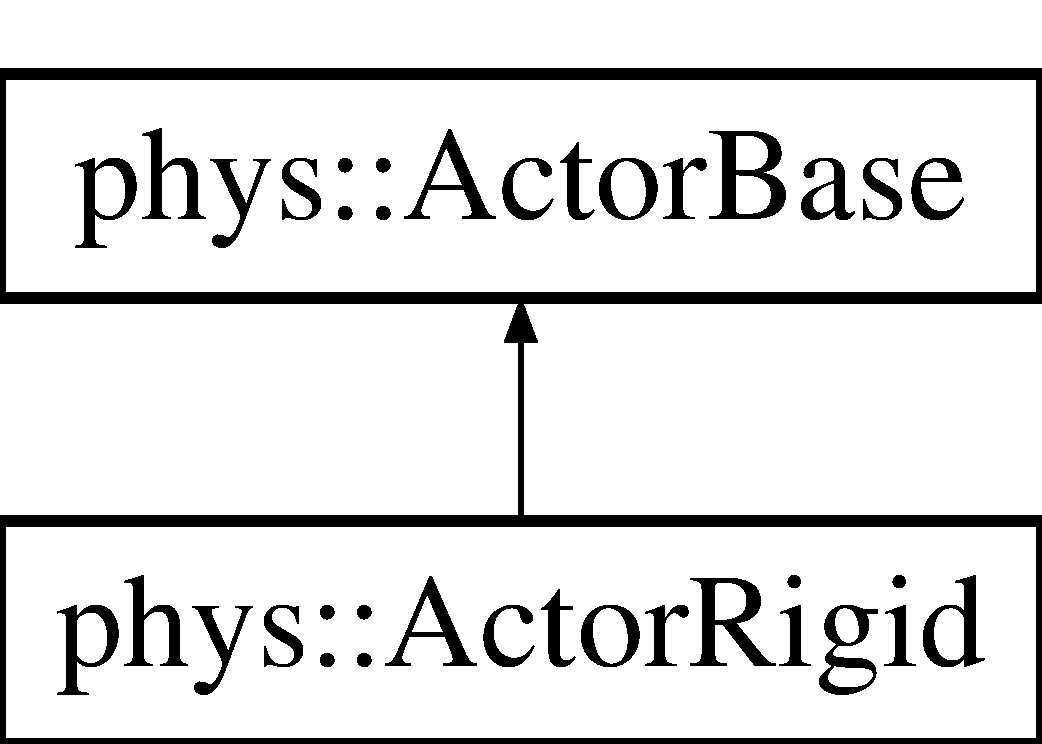
\includegraphics[height=2cm]{d8/d71/classphys_1_1ActorRigid}
\end{center}
\end{figure}
\subsection*{Public Member Functions}
\begin{DoxyCompactItemize}
\item 
\hyperlink{classphys_1_1ActorRigid_ac42c05745d57eb5745de3f34e820b72d}{ActorRigid} (\hyperlink{namespacephys_af7eb897198d265b8e868f45240230d5f}{Real} mass, \hyperlink{namespacephys_aa03900411993de7fbfec4789bc1d392e}{String} name, \hyperlink{namespacephys_aa03900411993de7fbfec4789bc1d392e}{String} file, \hyperlink{namespacephys_aa03900411993de7fbfec4789bc1d392e}{String} group, \hyperlink{classphys_1_1World}{World} $\ast$\_\-World)
\begin{DoxyCompactList}\small\item\em Descriptive constructor. \item\end{DoxyCompactList}\item 
virtual \hyperlink{classphys_1_1ActorRigid_ab317b5a2578157e54655a1aea8f4d058}{$\sim$ActorRigid} ()
\begin{DoxyCompactList}\small\item\em Destructor. \item\end{DoxyCompactList}\item 
void \hyperlink{classphys_1_1ActorRigid_aab4a408ce0724be6adf4c9f51f55f8a1}{CreateShapeFromMeshDynamic} (short unsigned int accuracy=1)
\begin{DoxyCompactList}\small\item\em Creates a collision shape from mesh file. \item\end{DoxyCompactList}\item 
void \hyperlink{classphys_1_1ActorRigid_a84554dcaaf2475ba0ec7dcb9235050ac}{CreateShapeFromMeshStatic} ()
\begin{DoxyCompactList}\small\item\em Creates a collision shape from mesh file. \item\end{DoxyCompactList}\item 
void \hyperlink{classphys_1_1ActorRigid_adaed962ee8ed788612e541fb00867c78}{LimitMovementOnAxis} (bool x, bool y, bool z)
\begin{DoxyCompactList}\small\item\em Restricts movement on the axis or axies of your choice. \item\end{DoxyCompactList}\end{DoxyCompactItemize}
\subsection*{Protected Member Functions}
\begin{DoxyCompactItemize}
\item 
void \hyperlink{classphys_1_1ActorRigid_a19227c52b972cd96ad69a7b6273e2bbf}{CreateRigidObject} (\hyperlink{namespacephys_af7eb897198d265b8e868f45240230d5f}{Real} pmass)
\begin{DoxyCompactList}\small\item\em Creates a rigid object for the actor. \item\end{DoxyCompactList}\item 
void \hyperlink{classphys_1_1ActorRigid_a3c56eb06fe6a7d468b7a67c45ade7be4}{AddObjectToWorld} (\hyperlink{classphys_1_1World}{World} $\ast$TargetWorld, btSoftRigidDynamicsWorld $\ast$btWorld)
\begin{DoxyCompactList}\small\item\em Adds the actor to the physics world. \item\end{DoxyCompactList}\end{DoxyCompactItemize}
\subsection*{Protected Attributes}
\begin{DoxyCompactItemize}
\item 
\hypertarget{classphys_1_1ActorRigid_a690889f942e177644f4f8521f509c88d}{
btRigidBody $\ast$ \hyperlink{classphys_1_1ActorRigid_a690889f942e177644f4f8521f509c88d}{physrigidbody}}
\label{d8/d71/classphys_1_1ActorRigid_a690889f942e177644f4f8521f509c88d}

\begin{DoxyCompactList}\small\item\em Used to simulate the behavior of a btRigidBody. \item\end{DoxyCompactList}\end{DoxyCompactItemize}


\subsection{Detailed Description}
This is the actor class for Rigid Objects. This class should be used to make any rigid object that can be moved as a result of force. Most objects will fall into this catagory. A few examples of a Rigid Object: Boxes, Car Frames, Chairs, etc. For Semi Rigid bodies that are deformable, like jello, it is better to use \hyperlink{classphys_1_1ActorSoft}{ActorSoft}. 

Definition at line 87 of file actorrigid.h.



\subsection{Constructor \& Destructor Documentation}
\hypertarget{classphys_1_1ActorRigid_ac42c05745d57eb5745de3f34e820b72d}{
\index{phys::ActorRigid@{phys::ActorRigid}!ActorRigid@{ActorRigid}}
\index{ActorRigid@{ActorRigid}!phys::ActorRigid@{phys::ActorRigid}}
\subsubsection[{ActorRigid}]{\setlength{\rightskip}{0pt plus 5cm}phys::ActorRigid::ActorRigid ({\bf Real} {\em mass}, \/  {\bf String} {\em name}, \/  {\bf String} {\em file}, \/  {\bf String} {\em group}, \/  {\bf World} $\ast$ {\em \_\-World})}}
\label{d8/d71/classphys_1_1ActorRigid_ac42c05745d57eb5745de3f34e820b72d}


Descriptive constructor. 

This constructor contains the basic information needed to make a Rigid Object. \par
 This class inherits from \hyperlink{classphys_1_1ActorBase}{ActorBase}. 
\begin{DoxyParams}{Parameters}
\item[{\em mass}]The mass the object will have in the \hyperlink{classphys_1_1World}{World}. \item[{\em name}]The name of the actor. \item[{\em file}]The 3d mesh file that contains the 3d model the actor will use. \item[{\em group}]The resource group where the 3d mesh and other related files can be found. \item[{\em \_\-World}]Pointer to the \hyperlink{classphys_1_1World}{World} this object will be added to. \end{DoxyParams}


Definition at line 53 of file actorrigid.cpp.

\hypertarget{classphys_1_1ActorRigid_ab317b5a2578157e54655a1aea8f4d058}{
\index{phys::ActorRigid@{phys::ActorRigid}!$\sim$ActorRigid@{$\sim$ActorRigid}}
\index{$\sim$ActorRigid@{$\sim$ActorRigid}!phys::ActorRigid@{phys::ActorRigid}}
\subsubsection[{$\sim$ActorRigid}]{\setlength{\rightskip}{0pt plus 5cm}phys::ActorRigid::$\sim$ActorRigid ()\hspace{0.3cm}{\ttfamily  \mbox{[}virtual\mbox{]}}}}
\label{d8/d71/classphys_1_1ActorRigid_ab317b5a2578157e54655a1aea8f4d058}


Destructor. 

The class destructor. 

Definition at line 58 of file actorrigid.cpp.



\subsection{Member Function Documentation}
\hypertarget{classphys_1_1ActorRigid_a3c56eb06fe6a7d468b7a67c45ade7be4}{
\index{phys::ActorRigid@{phys::ActorRigid}!AddObjectToWorld@{AddObjectToWorld}}
\index{AddObjectToWorld@{AddObjectToWorld}!phys::ActorRigid@{phys::ActorRigid}}
\subsubsection[{AddObjectToWorld}]{\setlength{\rightskip}{0pt plus 5cm}void phys::ActorRigid::AddObjectToWorld ({\bf World} $\ast$ {\em TargetWorld}, \/  btSoftRigidDynamicsWorld $\ast$ {\em btWorld})\hspace{0.3cm}{\ttfamily  \mbox{[}protected, virtual\mbox{]}}}}
\label{d8/d71/classphys_1_1ActorRigid_a3c56eb06fe6a7d468b7a67c45ade7be4}


Adds the actor to the physics world. 

Adds the actor to the physics world. \par
 This is automaticly called by the PhysWorlds AddActor function and shouldn't be called manually. 
\begin{DoxyParams}{Parameters}
\item[{\em TargetWorld}]Pointer to the \hyperlink{classphys_1_1World}{World} class. \item[{\em btWorld}]Pointer to the physics world. \end{DoxyParams}


Implements \hyperlink{classphys_1_1ActorBase_ac5d4ad5a634b16000742f506ed5957fb}{phys::ActorBase}.



Definition at line 70 of file actorrigid.cpp.

\hypertarget{classphys_1_1ActorRigid_a19227c52b972cd96ad69a7b6273e2bbf}{
\index{phys::ActorRigid@{phys::ActorRigid}!CreateRigidObject@{CreateRigidObject}}
\index{CreateRigidObject@{CreateRigidObject}!phys::ActorRigid@{phys::ActorRigid}}
\subsubsection[{CreateRigidObject}]{\setlength{\rightskip}{0pt plus 5cm}void phys::ActorRigid::CreateRigidObject ({\bf Real} {\em pmass})\hspace{0.3cm}{\ttfamily  \mbox{[}protected\mbox{]}}}}
\label{d8/d71/classphys_1_1ActorRigid_a19227c52b972cd96ad69a7b6273e2bbf}


Creates a rigid object for the actor. 

Creates a rigid object to be placed in the physics world later. \par
 This is automaticly called by the Constructor and shouldn't be called manually. 
\begin{DoxyParams}{Parameters}
\item[{\em pmass}]\char`\"{}Real Mass\char`\"{} The mass of the object. \end{DoxyParams}


Definition at line 63 of file actorrigid.cpp.

\hypertarget{classphys_1_1ActorRigid_aab4a408ce0724be6adf4c9f51f55f8a1}{
\index{phys::ActorRigid@{phys::ActorRigid}!CreateShapeFromMeshDynamic@{CreateShapeFromMeshDynamic}}
\index{CreateShapeFromMeshDynamic@{CreateShapeFromMeshDynamic}!phys::ActorRigid@{phys::ActorRigid}}
\subsubsection[{CreateShapeFromMeshDynamic}]{\setlength{\rightskip}{0pt plus 5cm}void phys::ActorRigid::CreateShapeFromMeshDynamic (short unsigned int {\em accuracy} = {\ttfamily 1})\hspace{0.3cm}{\ttfamily  \mbox{[}virtual\mbox{]}}}}
\label{d8/d71/classphys_1_1ActorRigid_aab4a408ce0724be6adf4c9f51f55f8a1}


Creates a collision shape from mesh file. 

This function will read the location of every verticy in the mesh file and use that to construct a triangle mesh shape and attach it to this objects collision shape. This shoiuld be used with only with Dynamic objects. 
\begin{DoxyParams}{Parameters}
\item[{\em accuracy}]A value from 1 to 4. The higher the more accurate, but the more resource intensive \end{DoxyParams}


\begin{Desc}
\item[\hyperlink{todo__todo000001}{Todo}]
\begin{DoxyItemize}
\item Check for thread safety 
\end{DoxyItemize}\end{Desc}


\begin{Desc}
\item[\hyperlink{todo__todo000002}{Todo}]add code here to increase the verticies that is used to create the hull from the first accuracy setting. \end{Desc}


\begin{Desc}
\item[\hyperlink{todo__todo000003}{Todo}]add code here for compound shapes of convex hulls \end{Desc}




Implements \hyperlink{classphys_1_1ActorBase_aa41370f6d2031a9dad8df45bd7f3bcc6}{phys::ActorBase}.



Definition at line 76 of file actorrigid.cpp.

\hypertarget{classphys_1_1ActorRigid_a84554dcaaf2475ba0ec7dcb9235050ac}{
\index{phys::ActorRigid@{phys::ActorRigid}!CreateShapeFromMeshStatic@{CreateShapeFromMeshStatic}}
\index{CreateShapeFromMeshStatic@{CreateShapeFromMeshStatic}!phys::ActorRigid@{phys::ActorRigid}}
\subsubsection[{CreateShapeFromMeshStatic}]{\setlength{\rightskip}{0pt plus 5cm}void phys::ActorRigid::CreateShapeFromMeshStatic ()}}
\label{d8/d71/classphys_1_1ActorRigid_a84554dcaaf2475ba0ec7dcb9235050ac}


Creates a collision shape from mesh file. 

This function will read the location of every verticy in the mesh file and use that to construct a triangle mesh shape and attach it to this objects collision shape. This shoiuld be used with only with Dynamic objects. 

\begin{Desc}
\item[\hyperlink{todo__todo000004}{Todo}]
\begin{DoxyItemize}
\item Check for thread safety 
\end{DoxyItemize}\end{Desc}




Definition at line 139 of file actorrigid.cpp.

\hypertarget{classphys_1_1ActorRigid_adaed962ee8ed788612e541fb00867c78}{
\index{phys::ActorRigid@{phys::ActorRigid}!LimitMovementOnAxis@{LimitMovementOnAxis}}
\index{LimitMovementOnAxis@{LimitMovementOnAxis}!phys::ActorRigid@{phys::ActorRigid}}
\subsubsection[{LimitMovementOnAxis}]{\setlength{\rightskip}{0pt plus 5cm}void phys::ActorRigid::LimitMovementOnAxis (bool {\em x}, \/  bool {\em y}, \/  bool {\em z})}}
\label{d8/d71/classphys_1_1ActorRigid_adaed962ee8ed788612e541fb00867c78}


Restricts movement on the axis or axies of your choice. 

This function will lock any and all axies you define you want to be locked. Simply pass true to allow movement on that axis, false if you don't. This function is primarily useful for 2D games, in which if you are viewing the playing area from the side you can pass in LimitMovementOnAxis(true,true,false) and the object will only be able to move up, down, or side to side, but not in or out. 
\begin{DoxyParams}{Parameters}
\item[{\em x}]Allow or Disallow use of the X axis for movement. \item[{\em y}]Allow or Disallow use of the Y axis for movement. \item[{\em z}]Allow or Disallow use of the Z axis for movement. \end{DoxyParams}


Definition at line 150 of file actorrigid.cpp.



The documentation for this class was generated from the following files:\begin{DoxyCompactItemize}
\item 
actorrigid.h\item 
actorrigid.cpp\end{DoxyCompactItemize}

\hypertarget{classphys_1_1ActorSoft}{
\section{phys::ActorSoft Class Reference}
\label{d4/d23/classphys_1_1ActorSoft}\index{phys::ActorSoft@{phys::ActorSoft}}
}


This is the actor class for Soft Objects.  




{\ttfamily \#include $<$physactor.h$>$}

Inheritance diagram for phys::ActorSoft:\begin{figure}[H]
\begin{center}
\leavevmode
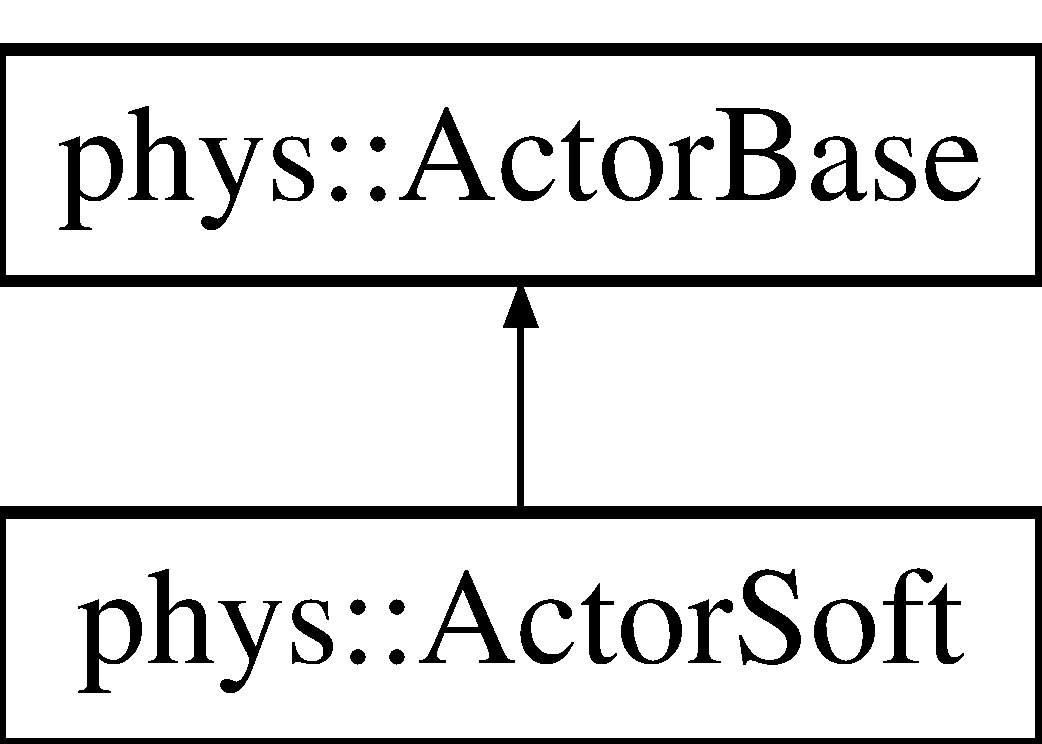
\includegraphics[height=2cm]{d4/d23/classphys_1_1ActorSoft}
\end{center}
\end{figure}
\subsection*{Public Member Functions}
\begin{DoxyCompactItemize}
\item 
virtual \hyperlink{classphys_1_1ActorSoft_a636c145f1e468fd45adc8da2a1708fbe}{$\sim$ActorSoft} ()
\begin{DoxyCompactList}\small\item\em Destructor. \item\end{DoxyCompactList}\item 
void \hyperlink{classphys_1_1ActorSoft_a51d78e0f503c3c815511c3d246b426ae}{CreateShapeFromMesh} ()
\begin{DoxyCompactList}\small\item\em Creates a collision shape from mesh file. \item\end{DoxyCompactList}\end{DoxyCompactItemize}
\subsection*{Protected Member Functions}
\begin{DoxyCompactItemize}
\item 
void \hyperlink{classphys_1_1ActorSoft_a04c98bb0ab9ed7c1dfc3435d49403ef4}{CreateSoftObject} (btSoftBodyWorldInfo $\ast$softworldinfo, int nodecount, btVector3 $\ast$nodearray, btScalar $\ast$massarray)
\begin{DoxyCompactList}\small\item\em Creates a soft object for the actor. \item\end{DoxyCompactList}\item 
void \hyperlink{classphys_1_1ActorSoft_a3a704ab32f847a5d0e060f8a592efefd}{AddObjectToWorld} (\hyperlink{classphys_1_1World}{World} $\ast$TargetWorld, btSoftRigidDynamicsWorld $\ast$btWorld)
\begin{DoxyCompactList}\small\item\em Adds the actor to the physics world. \item\end{DoxyCompactList}\end{DoxyCompactItemize}
\subsection*{Protected Attributes}
\begin{DoxyCompactItemize}
\item 
\hypertarget{classphys_1_1ActorSoft_ab3b2c8e1f94dff3e3244a5024595afef}{
btSoftBody $\ast$ \hyperlink{classphys_1_1ActorSoft_ab3b2c8e1f94dff3e3244a5024595afef}{physsoftbody}}
\label{d4/d23/classphys_1_1ActorSoft_ab3b2c8e1f94dff3e3244a5024595afef}

\begin{DoxyCompactList}\small\item\em Used to simulate the functionality of a btSoftBody for use with the physics subsystem. \item\end{DoxyCompactList}\end{DoxyCompactItemize}


\subsection{Detailed Description}
This is the actor class for Soft Objects. This class should be used to make any soft object that, like \hyperlink{classphys_1_1ActorRigid}{ActorRigid}, can be moved or manipulated as a result of force. Examples of soft objects are: Paper, Rope, and Cloth. Semi Rigid bodies that are still somewhat deformable, like Jello, should be made as a soft object. 

Definition at line 310 of file physactor.h.



\subsection{Constructor \& Destructor Documentation}
\hypertarget{classphys_1_1ActorSoft_a636c145f1e468fd45adc8da2a1708fbe}{
\index{phys::ActorSoft@{phys::ActorSoft}!$\sim$ActorSoft@{$\sim$ActorSoft}}
\index{$\sim$ActorSoft@{$\sim$ActorSoft}!phys::ActorSoft@{phys::ActorSoft}}
\subsubsection[{$\sim$ActorSoft}]{\setlength{\rightskip}{0pt plus 5cm}phys::ActorSoft::$\sim$ActorSoft ()\hspace{0.3cm}{\ttfamily  \mbox{[}virtual\mbox{]}}}}
\label{d4/d23/classphys_1_1ActorSoft_a636c145f1e468fd45adc8da2a1708fbe}


Destructor. 

The class destructor. 

Definition at line 458 of file physactor.cpp.



\subsection{Member Function Documentation}
\hypertarget{classphys_1_1ActorSoft_a3a704ab32f847a5d0e060f8a592efefd}{
\index{phys::ActorSoft@{phys::ActorSoft}!AddObjectToWorld@{AddObjectToWorld}}
\index{AddObjectToWorld@{AddObjectToWorld}!phys::ActorSoft@{phys::ActorSoft}}
\subsubsection[{AddObjectToWorld}]{\setlength{\rightskip}{0pt plus 5cm}void phys::ActorSoft::AddObjectToWorld ({\bf World} $\ast$ {\em TargetWorld}, \/  btSoftRigidDynamicsWorld $\ast$ {\em btWorld})\hspace{0.3cm}{\ttfamily  \mbox{[}protected, virtual\mbox{]}}}}
\label{d4/d23/classphys_1_1ActorSoft_a3a704ab32f847a5d0e060f8a592efefd}


Adds the actor to the physics world. 

Adds the actor to the physics world. \par
 This is automaticly called by the PhysWorlds AddActor function and shouldn't be called manually. 
\begin{DoxyParams}{Parameters}
\item[{\em TargetWorld}]Pointer to the \hyperlink{classphys_1_1World}{World} class. \item[{\em btWorld}]Pointer to the physics world. \end{DoxyParams}


Implements \hyperlink{classphys_1_1ActorBase_ac5d4ad5a634b16000742f506ed5957fb}{phys::ActorBase}.



Definition at line 469 of file physactor.cpp.

\hypertarget{classphys_1_1ActorSoft_a51d78e0f503c3c815511c3d246b426ae}{
\index{phys::ActorSoft@{phys::ActorSoft}!CreateShapeFromMesh@{CreateShapeFromMesh}}
\index{CreateShapeFromMesh@{CreateShapeFromMesh}!phys::ActorSoft@{phys::ActorSoft}}
\subsubsection[{CreateShapeFromMesh}]{\setlength{\rightskip}{0pt plus 5cm}void phys::ActorSoft::CreateShapeFromMesh ()}}
\label{d4/d23/classphys_1_1ActorSoft_a51d78e0f503c3c815511c3d246b426ae}


Creates a collision shape from mesh file. 

This function will read the location of every verticy in the mesh file and use that to construct a triangle mesh shape and attach it to this objects collision shape. 

Definition at line 474 of file physactor.cpp.

\hypertarget{classphys_1_1ActorSoft_a04c98bb0ab9ed7c1dfc3435d49403ef4}{
\index{phys::ActorSoft@{phys::ActorSoft}!CreateSoftObject@{CreateSoftObject}}
\index{CreateSoftObject@{CreateSoftObject}!phys::ActorSoft@{phys::ActorSoft}}
\subsubsection[{CreateSoftObject}]{\setlength{\rightskip}{0pt plus 5cm}void phys::ActorSoft::CreateSoftObject (btSoftBodyWorldInfo $\ast$ {\em softworldinfo}, \/  int {\em nodecount}, \/  btVector3 $\ast$ {\em nodearray}, \/  btScalar $\ast$ {\em massarray})\hspace{0.3cm}{\ttfamily  \mbox{[}protected\mbox{]}}}}
\label{d4/d23/classphys_1_1ActorSoft_a04c98bb0ab9ed7c1dfc3435d49403ef4}


Creates a soft object for the actor. 

Creates a soft object to be placed in the physics world later. \par
 This is automaticly called by the Constructor and shouldn't be called manually. 
\begin{DoxyParams}{Parameters}
\item[{\em softworldinfo}]Currently Unused \item[{\em nodecount}]Currently Unused \item[{\em nodearray}]Currently Unused \item[{\em massarray}]Currently Unused \end{DoxyParams}


Definition at line 463 of file physactor.cpp.



The documentation for this class was generated from the following files:\begin{DoxyCompactItemize}
\item 
physactor.h\item 
physactor.cpp\end{DoxyCompactItemize}

\hypertarget{classphys_1_1CallBackManager}{
\section{phys::CallBackManager Class Reference}
\label{d1/d47/classphys_1_1CallBackManager}\index{phys::CallBackManager@{phys::CallBackManager}}
}


This Stores callbacks for for use in the main loop.  




{\ttfamily \#include $<$callbackmanager.h$>$}

\subsection*{Public Member Functions}
\begin{DoxyCompactItemize}
\item 
\hyperlink{classphys_1_1CallBackManager_a16d4c60beef774ae904cf01853d71aae}{CallBackManager} (\hyperlink{classphys_1_1World}{World} $\ast$\_\-Parent)
\begin{DoxyCompactList}\small\item\em Constructor. \item\end{DoxyCompactList}\item 
\hyperlink{classphys_1_1CallBackManager_a098b7a7822538aa6d6c4ba690f1e069d}{$\sim$CallBackManager} ()
\begin{DoxyCompactList}\small\item\em Deconstructor. \item\end{DoxyCompactList}\item 
bool \hyperlink{classphys_1_1CallBackManager_a84e782f8729f49b296691763351ee2b1}{PreInput} ()
\begin{DoxyCompactList}\small\item\em This calls the PreInput Callback. \item\end{DoxyCompactList}\item 
void \hyperlink{classphys_1_1CallBackManager_ae3da6f1eb10cdf4d8551aaeeda73053c}{ErasePreInput} ()
\begin{DoxyCompactList}\small\item\em Drops the PreInput pointer. \item\end{DoxyCompactList}\item 
void \hyperlink{classphys_1_1CallBackManager_a1efb0c185304376986093beebf08a277}{SetPreInput} (bool($\ast$Callback)())
\begin{DoxyCompactList}\small\item\em This assigns a function to be the callback function for PreInput. \item\end{DoxyCompactList}\item 
bool \hyperlink{classphys_1_1CallBackManager_a1add8e6e7f5862ec4a4fe48095dc3c4e}{IsPreInputCallbackSet} ()
\begin{DoxyCompactList}\small\item\em Is the PreInput callback set or not. \item\end{DoxyCompactList}\item 
bool \hyperlink{classphys_1_1CallBackManager_a83afb36cfc7e71863d68a8b4c1d5e9d2}{PostInput} ()
\begin{DoxyCompactList}\small\item\em This calls the PostInput Callback. \item\end{DoxyCompactList}\item 
void \hyperlink{classphys_1_1CallBackManager_a84ccf382be58b42439869ec9b77a0f89}{ErasePostInput} ()
\begin{DoxyCompactList}\small\item\em Drops the PostInput pointer. \item\end{DoxyCompactList}\item 
void \hyperlink{classphys_1_1CallBackManager_abbf73a7199a64d6a2a39c7de44c5acd6}{SetPostInput} (bool($\ast$Callback)())
\begin{DoxyCompactList}\small\item\em This assigns a function to be the callback function for PostInput. \item\end{DoxyCompactList}\item 
bool \hyperlink{classphys_1_1CallBackManager_a075b799a815a2be2a83e30bb689711a7}{IsPostInputCallbackSet} ()
\begin{DoxyCompactList}\small\item\em Is the PostInput callback set or not. \item\end{DoxyCompactList}\item 
bool \hyperlink{classphys_1_1CallBackManager_a65867cc4855f0f8cd84a2b4a8bbf0fd6}{PrePhysics} ()
\begin{DoxyCompactList}\small\item\em This calls the PrePhysics Callback. \item\end{DoxyCompactList}\item 
void \hyperlink{classphys_1_1CallBackManager_afaeba4d6ae245d1560b76799417cce40}{ErasePrePhysics} ()
\begin{DoxyCompactList}\small\item\em Drops the PrePhysics pointer. \item\end{DoxyCompactList}\item 
void \hyperlink{classphys_1_1CallBackManager_a3f06ccacd416b3109f20c30cd30f9efe}{SetPrePhysics} (bool($\ast$Callback)())
\begin{DoxyCompactList}\small\item\em This assigns a function to be the callback function for PrePhysics. \item\end{DoxyCompactList}\item 
bool \hyperlink{classphys_1_1CallBackManager_af93b7b96e85faa77ed005840e0189ebd}{IsPrePhysicsCallbackSet} ()
\begin{DoxyCompactList}\small\item\em Is the PrePhysics callback set or not. \item\end{DoxyCompactList}\item 
bool \hyperlink{classphys_1_1CallBackManager_a06bf0e8787f21caf31bf428727155084}{PostPhysics} ()
\begin{DoxyCompactList}\small\item\em This calls the PostPhysics Callback. \item\end{DoxyCompactList}\item 
void \hyperlink{classphys_1_1CallBackManager_a2d03573a93606e9d3fcd7adad5c8c397}{ErasePostPhysics} ()
\begin{DoxyCompactList}\small\item\em Drops the PostPhysics pointer. \item\end{DoxyCompactList}\item 
void \hyperlink{classphys_1_1CallBackManager_a17687cd04807dfc80a25847be830c2f2}{SetPostPhysics} (bool($\ast$Callback)())
\begin{DoxyCompactList}\small\item\em This assigns a function to be the callback function for PostPhysics. \item\end{DoxyCompactList}\item 
bool \hyperlink{classphys_1_1CallBackManager_ac4bf07f907b8d4d7e052126bcfbba4ba}{IsPostPhysicsCallbackSet} ()
\begin{DoxyCompactList}\small\item\em Is the PostPhysics callback set or not. \item\end{DoxyCompactList}\item 
bool \hyperlink{classphys_1_1CallBackManager_a244c88b8a06f68a4f4bcff6253bf6806}{PreRender} ()
\begin{DoxyCompactList}\small\item\em This calls the PreRender Callback. \item\end{DoxyCompactList}\item 
void \hyperlink{classphys_1_1CallBackManager_adadf16f3f38398c9593646416ef18499}{ErasePreRender} ()
\begin{DoxyCompactList}\small\item\em Drops the PreRender pointer. \item\end{DoxyCompactList}\item 
void \hyperlink{classphys_1_1CallBackManager_a1e060fd479413457a798ea3c6b2bcb4d}{SetPreRender} (bool($\ast$Callback)())
\begin{DoxyCompactList}\small\item\em This assigns a function to be the callback function for PreRender. \item\end{DoxyCompactList}\item 
bool \hyperlink{classphys_1_1CallBackManager_aa4eff76517403726c846911f6b97b2c2}{IsPreRenderCallbackSet} ()
\begin{DoxyCompactList}\small\item\em Is the PreRender callback set or not. \item\end{DoxyCompactList}\item 
bool \hyperlink{classphys_1_1CallBackManager_aa1a1132e877d989ecea08a16ee4b3ac1}{PostRender} ()
\begin{DoxyCompactList}\small\item\em This calls the PostRender Callback. \item\end{DoxyCompactList}\item 
void \hyperlink{classphys_1_1CallBackManager_a0eef22a8df4dc87289a18f0e6a1d0baf}{ErasePostRender} ()
\begin{DoxyCompactList}\small\item\em Drops the PostRender pointer. \item\end{DoxyCompactList}\item 
void \hyperlink{classphys_1_1CallBackManager_afe6a91491f3872599d2c5784a902361a}{SetPostRender} (bool($\ast$Callback)())
\begin{DoxyCompactList}\small\item\em This assigns a function to be the callback function for PostRender. \item\end{DoxyCompactList}\item 
bool \hyperlink{classphys_1_1CallBackManager_a13011f2f9ffd561255772bc4082b304f}{IsPostRenderCallbackSet} ()
\begin{DoxyCompactList}\small\item\em Is the PostRender callback set or not. \item\end{DoxyCompactList}\end{DoxyCompactItemize}


\subsection{Detailed Description}
This Stores callbacks for for use in the main loop. This stores a series of pointers to functions that the main loop will call. This can be swapped out at any point in time with another \hyperlink{classphys_1_1CallBackManager}{CallBackManager} to completely (or subtley) alter game behavior. In general 

Definition at line 55 of file callbackmanager.h.



\subsection{Constructor \& Destructor Documentation}
\hypertarget{classphys_1_1CallBackManager_a16d4c60beef774ae904cf01853d71aae}{
\index{phys::CallBackManager@{phys::CallBackManager}!CallBackManager@{CallBackManager}}
\index{CallBackManager@{CallBackManager}!phys::CallBackManager@{phys::CallBackManager}}
\subsubsection[{CallBackManager}]{\setlength{\rightskip}{0pt plus 5cm}phys::CallBackManager::CallBackManager ({\bf World} $\ast$ {\em \_\-Parent})}}
\label{d1/d47/classphys_1_1CallBackManager_a16d4c60beef774ae904cf01853d71aae}


Constructor. 

This creates a usable but empty \hyperlink{classphys_1_1CallBackManager}{CallBackManager} 
\begin{DoxyParams}{Parameters}
\item[{\em \_\-Parent}]This is a pointer to the world that this callback manager works with. \end{DoxyParams}


Definition at line 56 of file callbackmanager.cpp.

\hypertarget{classphys_1_1CallBackManager_a098b7a7822538aa6d6c4ba690f1e069d}{
\index{phys::CallBackManager@{phys::CallBackManager}!$\sim$CallBackManager@{$\sim$CallBackManager}}
\index{$\sim$CallBackManager@{$\sim$CallBackManager}!phys::CallBackManager@{phys::CallBackManager}}
\subsubsection[{$\sim$CallBackManager}]{\setlength{\rightskip}{0pt plus 5cm}phys::CallBackManager::$\sim$CallBackManager ()}}
\label{d1/d47/classphys_1_1CallBackManager_a098b7a7822538aa6d6c4ba690f1e069d}


Deconstructor. 

Deconstructor Currently doesn't do very much 

Definition at line 70 of file callbackmanager.cpp.



\subsection{Member Function Documentation}
\hypertarget{classphys_1_1CallBackManager_a84ccf382be58b42439869ec9b77a0f89}{
\index{phys::CallBackManager@{phys::CallBackManager}!ErasePostInput@{ErasePostInput}}
\index{ErasePostInput@{ErasePostInput}!phys::CallBackManager@{phys::CallBackManager}}
\subsubsection[{ErasePostInput}]{\setlength{\rightskip}{0pt plus 5cm}void phys::CallBackManager::ErasePostInput ()}}
\label{d1/d47/classphys_1_1CallBackManager_a84ccf382be58b42439869ec9b77a0f89}


Drops the PostInput pointer. 

Drops the PostInput pointer, this does not 'delete' the pointer, merely assigns it to zero. 

Definition at line 122 of file callbackmanager.cpp.

\hypertarget{classphys_1_1CallBackManager_a2d03573a93606e9d3fcd7adad5c8c397}{
\index{phys::CallBackManager@{phys::CallBackManager}!ErasePostPhysics@{ErasePostPhysics}}
\index{ErasePostPhysics@{ErasePostPhysics}!phys::CallBackManager@{phys::CallBackManager}}
\subsubsection[{ErasePostPhysics}]{\setlength{\rightskip}{0pt plus 5cm}void phys::CallBackManager::ErasePostPhysics ()}}
\label{d1/d47/classphys_1_1CallBackManager_a2d03573a93606e9d3fcd7adad5c8c397}


Drops the PostPhysics pointer. 

Drops the PostPhysics pointer, this does not 'delete' the pointer, merely assigns it to zero. 

Definition at line 184 of file callbackmanager.cpp.

\hypertarget{classphys_1_1CallBackManager_a0eef22a8df4dc87289a18f0e6a1d0baf}{
\index{phys::CallBackManager@{phys::CallBackManager}!ErasePostRender@{ErasePostRender}}
\index{ErasePostRender@{ErasePostRender}!phys::CallBackManager@{phys::CallBackManager}}
\subsubsection[{ErasePostRender}]{\setlength{\rightskip}{0pt plus 5cm}void phys::CallBackManager::ErasePostRender ()}}
\label{d1/d47/classphys_1_1CallBackManager_a0eef22a8df4dc87289a18f0e6a1d0baf}


Drops the PostRender pointer. 

Drops the PostRender pointer, this does not 'delete' the pointer, merely assigns it to zero. 

Definition at line 247 of file callbackmanager.cpp.

\hypertarget{classphys_1_1CallBackManager_ae3da6f1eb10cdf4d8551aaeeda73053c}{
\index{phys::CallBackManager@{phys::CallBackManager}!ErasePreInput@{ErasePreInput}}
\index{ErasePreInput@{ErasePreInput}!phys::CallBackManager@{phys::CallBackManager}}
\subsubsection[{ErasePreInput}]{\setlength{\rightskip}{0pt plus 5cm}void phys::CallBackManager::ErasePreInput ()}}
\label{d1/d47/classphys_1_1CallBackManager_ae3da6f1eb10cdf4d8551aaeeda73053c}


Drops the PreInput pointer. 

Drops the PreInput pointer, this does not 'delete' the pointer, merely assigns it to zero. 

Definition at line 89 of file callbackmanager.cpp.

\hypertarget{classphys_1_1CallBackManager_afaeba4d6ae245d1560b76799417cce40}{
\index{phys::CallBackManager@{phys::CallBackManager}!ErasePrePhysics@{ErasePrePhysics}}
\index{ErasePrePhysics@{ErasePrePhysics}!phys::CallBackManager@{phys::CallBackManager}}
\subsubsection[{ErasePrePhysics}]{\setlength{\rightskip}{0pt plus 5cm}void phys::CallBackManager::ErasePrePhysics ()}}
\label{d1/d47/classphys_1_1CallBackManager_afaeba4d6ae245d1560b76799417cce40}


Drops the PrePhysics pointer. 

Drops the PrePhysics pointer, this does not 'delete' the pointer, merely assigns it to zero. 

Definition at line 153 of file callbackmanager.cpp.

\hypertarget{classphys_1_1CallBackManager_adadf16f3f38398c9593646416ef18499}{
\index{phys::CallBackManager@{phys::CallBackManager}!ErasePreRender@{ErasePreRender}}
\index{ErasePreRender@{ErasePreRender}!phys::CallBackManager@{phys::CallBackManager}}
\subsubsection[{ErasePreRender}]{\setlength{\rightskip}{0pt plus 5cm}void phys::CallBackManager::ErasePreRender ()}}
\label{d1/d47/classphys_1_1CallBackManager_adadf16f3f38398c9593646416ef18499}


Drops the PreRender pointer. 

Drops the PreRender pointer, this does not 'delete' the pointer, merely assigns it to zero. 

Definition at line 215 of file callbackmanager.cpp.

\hypertarget{classphys_1_1CallBackManager_a075b799a815a2be2a83e30bb689711a7}{
\index{phys::CallBackManager@{phys::CallBackManager}!IsPostInputCallbackSet@{IsPostInputCallbackSet}}
\index{IsPostInputCallbackSet@{IsPostInputCallbackSet}!phys::CallBackManager@{phys::CallBackManager}}
\subsubsection[{IsPostInputCallbackSet}]{\setlength{\rightskip}{0pt plus 5cm}bool phys::CallBackManager::IsPostInputCallbackSet ()}}
\label{d1/d47/classphys_1_1CallBackManager_a075b799a815a2be2a83e30bb689711a7}


Is the PostInput callback set or not. 

Is the PostInput callback set or not. The returns true if set or false otherwise. \begin{DoxyReturn}{Returns}
This returns true if the PostInput CallBack is set, false otherwise 
\end{DoxyReturn}


Definition at line 132 of file callbackmanager.cpp.

\hypertarget{classphys_1_1CallBackManager_ac4bf07f907b8d4d7e052126bcfbba4ba}{
\index{phys::CallBackManager@{phys::CallBackManager}!IsPostPhysicsCallbackSet@{IsPostPhysicsCallbackSet}}
\index{IsPostPhysicsCallbackSet@{IsPostPhysicsCallbackSet}!phys::CallBackManager@{phys::CallBackManager}}
\subsubsection[{IsPostPhysicsCallbackSet}]{\setlength{\rightskip}{0pt plus 5cm}bool phys::CallBackManager::IsPostPhysicsCallbackSet ()}}
\label{d1/d47/classphys_1_1CallBackManager_ac4bf07f907b8d4d7e052126bcfbba4ba}


Is the PostPhysics callback set or not. 

Is the PostPhysics callback set or not. The returns true if set or false otherwise. \begin{DoxyReturn}{Returns}
This returns true if the PostPhysics CallBack is set, false otherwise 
\end{DoxyReturn}


Definition at line 194 of file callbackmanager.cpp.

\hypertarget{classphys_1_1CallBackManager_a13011f2f9ffd561255772bc4082b304f}{
\index{phys::CallBackManager@{phys::CallBackManager}!IsPostRenderCallbackSet@{IsPostRenderCallbackSet}}
\index{IsPostRenderCallbackSet@{IsPostRenderCallbackSet}!phys::CallBackManager@{phys::CallBackManager}}
\subsubsection[{IsPostRenderCallbackSet}]{\setlength{\rightskip}{0pt plus 5cm}bool phys::CallBackManager::IsPostRenderCallbackSet ()}}
\label{d1/d47/classphys_1_1CallBackManager_a13011f2f9ffd561255772bc4082b304f}


Is the PostRender callback set or not. 

Is the PostRender callback set or not. The returns true if set or false otherwise. \begin{DoxyReturn}{Returns}
This returns true if the PostRender CallBack is set, false otherwise 
\end{DoxyReturn}


Definition at line 257 of file callbackmanager.cpp.

\hypertarget{classphys_1_1CallBackManager_a1add8e6e7f5862ec4a4fe48095dc3c4e}{
\index{phys::CallBackManager@{phys::CallBackManager}!IsPreInputCallbackSet@{IsPreInputCallbackSet}}
\index{IsPreInputCallbackSet@{IsPreInputCallbackSet}!phys::CallBackManager@{phys::CallBackManager}}
\subsubsection[{IsPreInputCallbackSet}]{\setlength{\rightskip}{0pt plus 5cm}bool phys::CallBackManager::IsPreInputCallbackSet ()}}
\label{d1/d47/classphys_1_1CallBackManager_a1add8e6e7f5862ec4a4fe48095dc3c4e}


Is the PreInput callback set or not. 

Is the PreInput callback set or not. The returns true if set or false otherwise. \begin{DoxyReturn}{Returns}
This returns true if the PreInput CallBack is set, false otherwise 
\end{DoxyReturn}


Definition at line 99 of file callbackmanager.cpp.

\hypertarget{classphys_1_1CallBackManager_af93b7b96e85faa77ed005840e0189ebd}{
\index{phys::CallBackManager@{phys::CallBackManager}!IsPrePhysicsCallbackSet@{IsPrePhysicsCallbackSet}}
\index{IsPrePhysicsCallbackSet@{IsPrePhysicsCallbackSet}!phys::CallBackManager@{phys::CallBackManager}}
\subsubsection[{IsPrePhysicsCallbackSet}]{\setlength{\rightskip}{0pt plus 5cm}bool phys::CallBackManager::IsPrePhysicsCallbackSet ()}}
\label{d1/d47/classphys_1_1CallBackManager_af93b7b96e85faa77ed005840e0189ebd}


Is the PrePhysics callback set or not. 

Is the PrePhysics callback set or not. The returns true if set or false otherwise. \begin{DoxyReturn}{Returns}
This returns true if the PrePhysics CallBack is set, false otherwise 
\end{DoxyReturn}


Definition at line 163 of file callbackmanager.cpp.

\hypertarget{classphys_1_1CallBackManager_aa4eff76517403726c846911f6b97b2c2}{
\index{phys::CallBackManager@{phys::CallBackManager}!IsPreRenderCallbackSet@{IsPreRenderCallbackSet}}
\index{IsPreRenderCallbackSet@{IsPreRenderCallbackSet}!phys::CallBackManager@{phys::CallBackManager}}
\subsubsection[{IsPreRenderCallbackSet}]{\setlength{\rightskip}{0pt plus 5cm}bool phys::CallBackManager::IsPreRenderCallbackSet ()}}
\label{d1/d47/classphys_1_1CallBackManager_aa4eff76517403726c846911f6b97b2c2}


Is the PreRender callback set or not. 

Is the PreRender callback set or not. The returns true if set or false otherwise. \begin{DoxyReturn}{Returns}
This returns true if the PreRender CallBack is set, false otherwise 
\end{DoxyReturn}


Definition at line 225 of file callbackmanager.cpp.

\hypertarget{classphys_1_1CallBackManager_a83afb36cfc7e71863d68a8b4c1d5e9d2}{
\index{phys::CallBackManager@{phys::CallBackManager}!PostInput@{PostInput}}
\index{PostInput@{PostInput}!phys::CallBackManager@{phys::CallBackManager}}
\subsubsection[{PostInput}]{\setlength{\rightskip}{0pt plus 5cm}bool phys::CallBackManager::PostInput ()}}
\label{d1/d47/classphys_1_1CallBackManager_a83afb36cfc7e71863d68a8b4c1d5e9d2}


This calls the PostInput Callback. 

This calls the PostInput Callback and returns true if the callback intends to continue with the mainloop, and false if the callback intend to end the mainloop. \begin{DoxyReturn}{Returns}
A bool that represents whether the mainloop should end. 
\end{DoxyReturn}


Definition at line 111 of file callbackmanager.cpp.

\hypertarget{classphys_1_1CallBackManager_a06bf0e8787f21caf31bf428727155084}{
\index{phys::CallBackManager@{phys::CallBackManager}!PostPhysics@{PostPhysics}}
\index{PostPhysics@{PostPhysics}!phys::CallBackManager@{phys::CallBackManager}}
\subsubsection[{PostPhysics}]{\setlength{\rightskip}{0pt plus 5cm}bool phys::CallBackManager::PostPhysics ()}}
\label{d1/d47/classphys_1_1CallBackManager_a06bf0e8787f21caf31bf428727155084}


This calls the PostPhysics Callback. 

This calls the PostPhysics Callback and returns true if the callback intends to continue with the mainloop, and false if the callback intend to end the mainloop. \begin{DoxyReturn}{Returns}
A bool that represents whether the mainloop should end. 
\end{DoxyReturn}


Definition at line 175 of file callbackmanager.cpp.

\hypertarget{classphys_1_1CallBackManager_aa1a1132e877d989ecea08a16ee4b3ac1}{
\index{phys::CallBackManager@{phys::CallBackManager}!PostRender@{PostRender}}
\index{PostRender@{PostRender}!phys::CallBackManager@{phys::CallBackManager}}
\subsubsection[{PostRender}]{\setlength{\rightskip}{0pt plus 5cm}bool phys::CallBackManager::PostRender ()}}
\label{d1/d47/classphys_1_1CallBackManager_aa1a1132e877d989ecea08a16ee4b3ac1}


This calls the PostRender Callback. 

This calls the PostRender Callback and returns true if the callback intends to continue with the mainloop, and false if the callback intend to end the mainloop. \begin{DoxyReturn}{Returns}
A bool that represents whether the mainloop should end. 
\end{DoxyReturn}


Definition at line 238 of file callbackmanager.cpp.

\hypertarget{classphys_1_1CallBackManager_a84e782f8729f49b296691763351ee2b1}{
\index{phys::CallBackManager@{phys::CallBackManager}!PreInput@{PreInput}}
\index{PreInput@{PreInput}!phys::CallBackManager@{phys::CallBackManager}}
\subsubsection[{PreInput}]{\setlength{\rightskip}{0pt plus 5cm}bool phys::CallBackManager::PreInput ()}}
\label{d1/d47/classphys_1_1CallBackManager_a84e782f8729f49b296691763351ee2b1}


This calls the PreInput Callback. 

This calls the PreInput Callback and returns true if the callback intends to continue with the mainloop, and false if the callback intend to end the mainloop. \begin{DoxyReturn}{Returns}
A bool that represents whether the mainloop should end. 
\end{DoxyReturn}


Definition at line 78 of file callbackmanager.cpp.

\hypertarget{classphys_1_1CallBackManager_a65867cc4855f0f8cd84a2b4a8bbf0fd6}{
\index{phys::CallBackManager@{phys::CallBackManager}!PrePhysics@{PrePhysics}}
\index{PrePhysics@{PrePhysics}!phys::CallBackManager@{phys::CallBackManager}}
\subsubsection[{PrePhysics}]{\setlength{\rightskip}{0pt plus 5cm}bool phys::CallBackManager::PrePhysics ()}}
\label{d1/d47/classphys_1_1CallBackManager_a65867cc4855f0f8cd84a2b4a8bbf0fd6}


This calls the PrePhysics Callback. 

This calls the PrePhysics Callback and returns true if the callback intends to continue with the mainloop, and false if the callback intend to end the mainloop. \begin{DoxyReturn}{Returns}
A bool that represents whether the mainloop should end. 
\end{DoxyReturn}


Definition at line 144 of file callbackmanager.cpp.

\hypertarget{classphys_1_1CallBackManager_a244c88b8a06f68a4f4bcff6253bf6806}{
\index{phys::CallBackManager@{phys::CallBackManager}!PreRender@{PreRender}}
\index{PreRender@{PreRender}!phys::CallBackManager@{phys::CallBackManager}}
\subsubsection[{PreRender}]{\setlength{\rightskip}{0pt plus 5cm}bool phys::CallBackManager::PreRender ()}}
\label{d1/d47/classphys_1_1CallBackManager_a244c88b8a06f68a4f4bcff6253bf6806}


This calls the PreRender Callback. 

This calls the PreRender Callback and returns true if the callback intends to continue with the mainloop, and false if the callback intend to end the mainloop. \begin{DoxyReturn}{Returns}
A bool that represents whether the mainloop should end. 
\end{DoxyReturn}


Definition at line 206 of file callbackmanager.cpp.

\hypertarget{classphys_1_1CallBackManager_abbf73a7199a64d6a2a39c7de44c5acd6}{
\index{phys::CallBackManager@{phys::CallBackManager}!SetPostInput@{SetPostInput}}
\index{SetPostInput@{SetPostInput}!phys::CallBackManager@{phys::CallBackManager}}
\subsubsection[{SetPostInput}]{\setlength{\rightskip}{0pt plus 5cm}void phys::CallBackManager::SetPostInput (bool($\ast$)() {\em Callback})}}
\label{d1/d47/classphys_1_1CallBackManager_abbf73a7199a64d6a2a39c7de44c5acd6}


This assigns a function to be the callback function for PostInput. 

This assigns a function to be the callback function for PostInput. 
\begin{DoxyParams}{Parameters}
\item[{\em Callback}]This is a pointer to a function that returns a bool and accepts no arguments \end{DoxyParams}


Definition at line 127 of file callbackmanager.cpp.

\hypertarget{classphys_1_1CallBackManager_a17687cd04807dfc80a25847be830c2f2}{
\index{phys::CallBackManager@{phys::CallBackManager}!SetPostPhysics@{SetPostPhysics}}
\index{SetPostPhysics@{SetPostPhysics}!phys::CallBackManager@{phys::CallBackManager}}
\subsubsection[{SetPostPhysics}]{\setlength{\rightskip}{0pt plus 5cm}void phys::CallBackManager::SetPostPhysics (bool($\ast$)() {\em Callback})}}
\label{d1/d47/classphys_1_1CallBackManager_a17687cd04807dfc80a25847be830c2f2}


This assigns a function to be the callback function for PostPhysics. 

This assigns a function to be the callback function for PostPhysics. 
\begin{DoxyParams}{Parameters}
\item[{\em Callback}]This is a pointer to a function that returns a bool and accepts no arguments \end{DoxyParams}


Definition at line 189 of file callbackmanager.cpp.

\hypertarget{classphys_1_1CallBackManager_afe6a91491f3872599d2c5784a902361a}{
\index{phys::CallBackManager@{phys::CallBackManager}!SetPostRender@{SetPostRender}}
\index{SetPostRender@{SetPostRender}!phys::CallBackManager@{phys::CallBackManager}}
\subsubsection[{SetPostRender}]{\setlength{\rightskip}{0pt plus 5cm}void phys::CallBackManager::SetPostRender (bool($\ast$)() {\em Callback})}}
\label{d1/d47/classphys_1_1CallBackManager_afe6a91491f3872599d2c5784a902361a}


This assigns a function to be the callback function for PostRender. 

This assigns a function to be the callback function for PostRender. 
\begin{DoxyParams}{Parameters}
\item[{\em Callback}]This is a pointer to a function that returns a bool and accepts no arguments \end{DoxyParams}


Definition at line 252 of file callbackmanager.cpp.

\hypertarget{classphys_1_1CallBackManager_a1efb0c185304376986093beebf08a277}{
\index{phys::CallBackManager@{phys::CallBackManager}!SetPreInput@{SetPreInput}}
\index{SetPreInput@{SetPreInput}!phys::CallBackManager@{phys::CallBackManager}}
\subsubsection[{SetPreInput}]{\setlength{\rightskip}{0pt plus 5cm}void phys::CallBackManager::SetPreInput (bool($\ast$)() {\em Callback})}}
\label{d1/d47/classphys_1_1CallBackManager_a1efb0c185304376986093beebf08a277}


This assigns a function to be the callback function for PreInput. 

This assigns a function to be the callback function for PreInput. 
\begin{DoxyParams}{Parameters}
\item[{\em Callback}]This is a pointer to a function that returns a bool and accepts no arguments \end{DoxyParams}


Definition at line 94 of file callbackmanager.cpp.

\hypertarget{classphys_1_1CallBackManager_a3f06ccacd416b3109f20c30cd30f9efe}{
\index{phys::CallBackManager@{phys::CallBackManager}!SetPrePhysics@{SetPrePhysics}}
\index{SetPrePhysics@{SetPrePhysics}!phys::CallBackManager@{phys::CallBackManager}}
\subsubsection[{SetPrePhysics}]{\setlength{\rightskip}{0pt plus 5cm}void phys::CallBackManager::SetPrePhysics (bool($\ast$)() {\em Callback})}}
\label{d1/d47/classphys_1_1CallBackManager_a3f06ccacd416b3109f20c30cd30f9efe}


This assigns a function to be the callback function for PrePhysics. 

This assigns a function to be the callback function for PrePhysics. 
\begin{DoxyParams}{Parameters}
\item[{\em Callback}]This is a pointer to a function that returns a bool and accepts no arguments \end{DoxyParams}


Definition at line 158 of file callbackmanager.cpp.

\hypertarget{classphys_1_1CallBackManager_a1e060fd479413457a798ea3c6b2bcb4d}{
\index{phys::CallBackManager@{phys::CallBackManager}!SetPreRender@{SetPreRender}}
\index{SetPreRender@{SetPreRender}!phys::CallBackManager@{phys::CallBackManager}}
\subsubsection[{SetPreRender}]{\setlength{\rightskip}{0pt plus 5cm}void phys::CallBackManager::SetPreRender (bool($\ast$)() {\em Callback})}}
\label{d1/d47/classphys_1_1CallBackManager_a1e060fd479413457a798ea3c6b2bcb4d}


This assigns a function to be the callback function for PreRender. 

This assigns a function to be the callback function for PreRender. 
\begin{DoxyParams}{Parameters}
\item[{\em Callback}]This is a pointer to a function that returns a bool and accepts no arguments \end{DoxyParams}


Definition at line 220 of file callbackmanager.cpp.



The documentation for this class was generated from the following files:\begin{DoxyCompactItemize}
\item 
callbackmanager.h\item 
callbackmanager.cpp\end{DoxyCompactItemize}

\hypertarget{classphys_1_1EventBase}{
\section{phys::EventBase Class Reference}
\label{dd/d80/classphys_1_1EventBase}\index{phys::EventBase@{phys::EventBase}}
}


The base class for all events.  




{\ttfamily \#include $<$eventbase.h$>$}

Inheritance diagram for phys::EventBase:\begin{figure}[H]
\begin{center}
\leavevmode
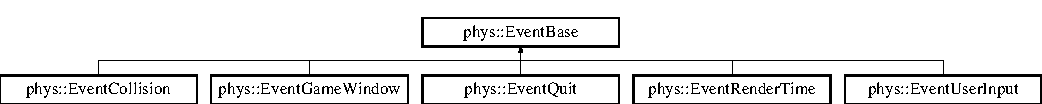
\includegraphics[height=1.842105cm]{dd/d80/classphys_1_1EventBase}
\end{center}
\end{figure}
\subsection*{Public Types}
\begin{DoxyCompactItemize}
\item 
enum \hyperlink{classphys_1_1EventBase_a5e6a8564e127f654123f0bf6a2751923}{EventType} \{ \par
\hyperlink{classphys_1_1EventBase_a5e6a8564e127f654123f0bf6a2751923acdfa47d279e8a1c460d557d14b85c7a5}{RenderTime}, 
\hyperlink{classphys_1_1EventBase_a5e6a8564e127f654123f0bf6a2751923a320cc0817dc2c2201501b12c50c89bef}{UserInput}, 
\hyperlink{classphys_1_1EventBase_a5e6a8564e127f654123f0bf6a2751923a84742ff55e9abdde8f5e0578d30f73a9}{QuitMessage}, 
\hyperlink{classphys_1_1EventBase_a5e6a8564e127f654123f0bf6a2751923a18594400c60af959158e9f5cc2cd5d08}{SystemMessage}, 
\par
\hyperlink{classphys_1_1EventBase_a5e6a8564e127f654123f0bf6a2751923adb6767503168d145497ef65a708725e5}{Collision}, 
{\bfseries Other}
 \}
\end{DoxyCompactItemize}
\subsection*{Public Member Functions}
\begin{DoxyCompactItemize}
\item 
virtual \hyperlink{classphys_1_1EventBase_a5e6a8564e127f654123f0bf6a2751923}{EventBase::EventType} \hyperlink{classphys_1_1EventBase_a1b3d29b6ecf30f18cc3e1825a515c508}{GetType} () const =0
\begin{DoxyCompactList}\small\item\em This will aid in identifying all classes that inherit from this class. \item\end{DoxyCompactList}\end{DoxyCompactItemize}


\subsection{Detailed Description}
The base class for all events. All Events used in the Event Manager, will inherit from this. While not absolutely required by the game programmer to write their own events, it it could be useful. Instances of this class cannot be made, and all classes that inherit from this are expected to implement getEventType(). 

Definition at line 61 of file eventbase.h.



\subsection{Member Enumeration Documentation}
\hypertarget{classphys_1_1EventBase_a5e6a8564e127f654123f0bf6a2751923}{
\index{phys::EventBase@{phys::EventBase}!EventType@{EventType}}
\index{EventType@{EventType}!phys::EventBase@{phys::EventBase}}
\subsubsection[{EventType}]{\setlength{\rightskip}{0pt plus 5cm}enum {\bf phys::EventBase::EventType}}}
\label{dd/d80/classphys_1_1EventBase_a5e6a8564e127f654123f0bf6a2751923}
A listing of values that can be used to identify Events. \begin{Desc}
\item[Enumerator: ]\par
\begin{description}
\index{RenderTime@{RenderTime}!phys::EventBase@{phys::EventBase}}\index{phys::EventBase@{phys::EventBase}!RenderTime@{RenderTime}}\item[{\em 
\hypertarget{classphys_1_1EventBase_a5e6a8564e127f654123f0bf6a2751923acdfa47d279e8a1c460d557d14b85c7a5}{
RenderTime}
\label{dd/d80/classphys_1_1EventBase_a5e6a8564e127f654123f0bf6a2751923acdfa47d279e8a1c460d557d14b85c7a5}
}]Indicates the Event is a PhysEventRenderTime \index{UserInput@{UserInput}!phys::EventBase@{phys::EventBase}}\index{phys::EventBase@{phys::EventBase}!UserInput@{UserInput}}\item[{\em 
\hypertarget{classphys_1_1EventBase_a5e6a8564e127f654123f0bf6a2751923a320cc0817dc2c2201501b12c50c89bef}{
UserInput}
\label{dd/d80/classphys_1_1EventBase_a5e6a8564e127f654123f0bf6a2751923a320cc0817dc2c2201501b12c50c89bef}
}]Indicates the Event is a \hyperlink{classphys_1_1EventUserInput}{EventUserInput} \index{QuitMessage@{QuitMessage}!phys::EventBase@{phys::EventBase}}\index{phys::EventBase@{phys::EventBase}!QuitMessage@{QuitMessage}}\item[{\em 
\hypertarget{classphys_1_1EventBase_a5e6a8564e127f654123f0bf6a2751923a84742ff55e9abdde8f5e0578d30f73a9}{
QuitMessage}
\label{dd/d80/classphys_1_1EventBase_a5e6a8564e127f654123f0bf6a2751923a84742ff55e9abdde8f5e0578d30f73a9}
}]Indicates the Event is a \hyperlink{classphys_1_1EventQuit}{phys::EventQuit} \index{SystemMessage@{SystemMessage}!phys::EventBase@{phys::EventBase}}\index{phys::EventBase@{phys::EventBase}!SystemMessage@{SystemMessage}}\item[{\em 
\hypertarget{classphys_1_1EventBase_a5e6a8564e127f654123f0bf6a2751923a18594400c60af959158e9f5cc2cd5d08}{
SystemMessage}
\label{dd/d80/classphys_1_1EventBase_a5e6a8564e127f654123f0bf6a2751923a18594400c60af959158e9f5cc2cd5d08}
}]Indicates the Event has not been coded yet \index{Collision@{Collision}!phys::EventBase@{phys::EventBase}}\index{phys::EventBase@{phys::EventBase}!Collision@{Collision}}\item[{\em 
\hypertarget{classphys_1_1EventBase_a5e6a8564e127f654123f0bf6a2751923adb6767503168d145497ef65a708725e5}{
Collision}
\label{dd/d80/classphys_1_1EventBase_a5e6a8564e127f654123f0bf6a2751923adb6767503168d145497ef65a708725e5}
}]Indicates the Event is a Physics Collision Event \end{description}
\end{Desc}



Definition at line 67 of file eventbase.h.



\subsection{Member Function Documentation}
\hypertarget{classphys_1_1EventBase_a1b3d29b6ecf30f18cc3e1825a515c508}{
\index{phys::EventBase@{phys::EventBase}!GetType@{GetType}}
\index{GetType@{GetType}!phys::EventBase@{phys::EventBase}}
\subsubsection[{GetType}]{\setlength{\rightskip}{0pt plus 5cm}virtual {\bf EventBase::EventType} phys::EventBase::GetType (
\begin{DoxyParamCaption}
{}
\end{DoxyParamCaption}
) const\hspace{0.3cm}{\ttfamily  \mbox{[}pure virtual\mbox{]}}}}
\label{dd/d80/classphys_1_1EventBase_a1b3d29b6ecf30f18cc3e1825a515c508}


This will aid in identifying all classes that inherit from this class. 

All Classes derived form this calls will return an Event::EventType that correspond the the data/class type they actually are. \begin{DoxyReturn}{Returns}
This returns an eventype that will correspend with the actual event type. This can be used on all Phys game provided class to safely cast a pointer to the correct event type. 
\end{DoxyReturn}


Implemented in \hyperlink{classphys_1_1EventCollision_a96c2809f1bbab78b9f2758cea15a9a36}{phys::EventCollision}, \hyperlink{classphys_1_1EventQuit_a3bfca875349e73dbda47c3c62a253e3b}{phys::EventQuit}, \hyperlink{classphys_1_1EventRenderTime_a160ca55bf9e5a2ae80dab82eab88baf5}{phys::EventRenderTime}, and \hyperlink{classphys_1_1EventUserInput_a3e803a8d9bcc1576fe04d2245a86ec80}{phys::EventUserInput}.



The documentation for this class was generated from the following file:\begin{DoxyCompactItemize}
\item 
eventbase.h\end{DoxyCompactItemize}

\hypertarget{classphys_1_1EventManager}{
\subsection{phys::EventManager Class Reference}
\label{classphys_1_1EventManager}\index{phys::EventManager@{phys::EventManager}}
}


This is a container for Events and facilitates the transfer of data.  




{\ttfamily \#include $<$eventmanager.h$>$}

Inheritance diagram for phys::EventManager:\begin{figure}[H]
\begin{center}
\leavevmode
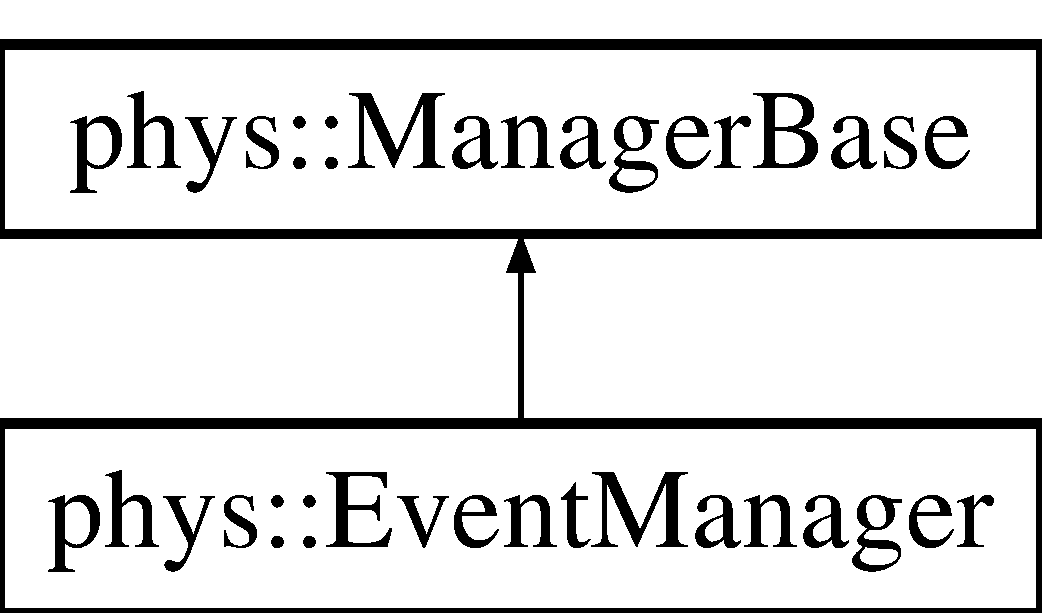
\includegraphics[height=2.000000cm]{classphys_1_1EventManager}
\end{center}
\end{figure}
\subsubsection*{Public Member Functions}
\begin{DoxyCompactItemize}
\item 
void \hyperlink{classphys_1_1EventManager_abada23d83ef38e59a38eb91a88a07404}{AddEvent} (\hyperlink{classphys_1_1EventBase}{EventBase} $\ast$EventToAdd)
\begin{DoxyCompactList}\small\item\em Adds an event of any kind to the end of the Event Queue. \item\end{DoxyCompactList}\item 
void \hyperlink{classphys_1_1EventManager_a6ff66883358344908afd11204f79f196}{AddPollingCheck} (const \hyperlink{classphys_1_1MetaCode}{MetaCode} \&InputToTryPolling)
\begin{DoxyCompactList}\small\item\em Generates extra events each iteration of the main loop, based on user input polling. \item\end{DoxyCompactList}\item 
void \hyperlink{classphys_1_1EventManager_a0b36c605c2a059c96e787ed4c1fd68bc}{DetectJoysticks} ()
\begin{DoxyCompactList}\small\item\em Look for Joysticks that are hooked up to the system. \item\end{DoxyCompactList}\item 
virtual void \hyperlink{classphys_1_1EventManager_aca8fb3d285484dcdb943824bf11f3596}{DoMainLoopItems} ()
\begin{DoxyCompactList}\small\item\em Empty MainLoopItems. \item\end{DoxyCompactList}\item 
\hyperlink{classphys_1_1EventManager_a018b36588bf2a2e90536e64be060d6fc}{EventManager} ()
\begin{DoxyCompactList}\small\item\em Default constructor. \item\end{DoxyCompactList}\item 
std::list$<$ \hyperlink{classphys_1_1EventCollision}{EventCollision} $\ast$ $>$ $\ast$ \hyperlink{classphys_1_1EventManager_a1881421e075a5965d6d5a0678f93ad9a}{GetAllCollisionEvents} ()
\begin{DoxyCompactList}\small\item\em This returns a complete list of all the Render \hyperlink{structphys_1_1Time}{Time} events. \item\end{DoxyCompactList}\item 
std::list$<$ \hyperlink{classphys_1_1EventGameWindow}{EventGameWindow} $\ast$ $>$ $\ast$ \hyperlink{classphys_1_1EventManager_aacdd185f6334f1258d0d7022bae3932d}{GetAllGameWindowEvents} ()
\begin{DoxyCompactList}\small\item\em This returns a complete list of all the Render \hyperlink{structphys_1_1Time}{Time} events. \item\end{DoxyCompactList}\item 
std::list$<$ \hyperlink{classphys_1_1EventQuit}{EventQuit} $\ast$ $>$ $\ast$ \hyperlink{classphys_1_1EventManager_afefd52a9693bc5541592997abbf3c53f}{GetAllQuitEvents} ()
\begin{DoxyCompactList}\small\item\em This returns a complete list of all the quit events. \item\end{DoxyCompactList}\item 
std::list$<$ \hyperlink{classphys_1_1EventRenderTime}{EventRenderTime} $\ast$ $>$ $\ast$ \hyperlink{classphys_1_1EventManager_aee73dff2d113826b8c01db7f7417d527}{GetAllRenderTimeEvents} ()
\begin{DoxyCompactList}\small\item\em This returns a complete list of all the Render \hyperlink{structphys_1_1Time}{Time} events. \item\end{DoxyCompactList}\item 
std::list$<$ \hyperlink{classphys_1_1EventBase}{EventBase} $\ast$ $>$ $\ast$ \hyperlink{classphys_1_1EventManager_a300e537d27cd53ac8276438d4c91a3f6}{GetAllSpecificEvents} (\hyperlink{classphys_1_1EventBase_a5e6a8564e127f654123f0bf6a2751923}{EventBase::EventType} SpecificType)
\begin{DoxyCompactList}\small\item\em This returns a complete list of all the specified events. \item\end{DoxyCompactList}\item 
std::list$<$ \hyperlink{classphys_1_1EventUserInput}{EventUserInput} $\ast$ $>$ $\ast$ \hyperlink{classphys_1_1EventManager_aef240dacae9479c4385d540e4feab867}{GetAllUserInputEvents} ()
\begin{DoxyCompactList}\small\item\em This returns a complete list of all the User Input events. \item\end{DoxyCompactList}\item 
\hyperlink{classphys_1_1EventCollision}{EventCollision} $\ast$ \hyperlink{classphys_1_1EventManager_a8e8f88684cd9167ae59734cf14b64b76}{GetNextCollisionEvent} ()
\begin{DoxyCompactList}\small\item\em Returns a pointer to the Next Collision event. \item\end{DoxyCompactList}\item 
\hyperlink{classphys_1_1EventBase}{EventBase} $\ast$ \hyperlink{classphys_1_1EventManager_aa0937763961aefc59aea197a8f9bc0dc}{GetNextEvent} ()
\begin{DoxyCompactList}\small\item\em Return a pointer to the Next event. \item\end{DoxyCompactList}\item 
\hyperlink{classphys_1_1EventGameWindow}{EventGameWindow} $\ast$ \hyperlink{classphys_1_1EventManager_aead881349edba3f0bcca34eaae41a8ee}{GetNextGameWindowEvent} ()
\begin{DoxyCompactList}\small\item\em Returns a pointer to the Next \hyperlink{classphys_1_1GameWindow}{GameWindow} event. \item\end{DoxyCompactList}\item 
\hyperlink{classphys_1_1EventQuit}{EventQuit} $\ast$ \hyperlink{classphys_1_1EventManager_ad7da09e5422b1db79ac4187ee9198d0c}{GetNextQuitEvent} ()
\begin{DoxyCompactList}\small\item\em Returns a pointer to the Next \hyperlink{classphys_1_1EventQuit}{EventQuit}. \item\end{DoxyCompactList}\item 
\hyperlink{classphys_1_1EventRenderTime}{EventRenderTime} $\ast$ \hyperlink{classphys_1_1EventManager_ae8730b039a280449af052d75f2e60b06}{GetNextRenderTimeEvent} ()
\begin{DoxyCompactList}\small\item\em Returns a pointer to the Next Rendertime event. \item\end{DoxyCompactList}\item 
\hyperlink{classphys_1_1EventBase}{EventBase} $\ast$ \hyperlink{classphys_1_1EventManager_a7340cfab326856cf4ebc653b11101016}{GetNextSpecificEvent} (\hyperlink{classphys_1_1EventBase_a5e6a8564e127f654123f0bf6a2751923}{EventBase::EventType} SpecificType)
\begin{DoxyCompactList}\small\item\em Returns a pointer to the Next kind event of the Specified type. \item\end{DoxyCompactList}\item 
\hyperlink{classphys_1_1EventUserInput}{EventUserInput} $\ast$ \hyperlink{classphys_1_1EventManager_a38b42602a3a4d621048c78b525b4db49}{GetNextUserInputEvent} ()
\begin{DoxyCompactList}\small\item\em Returns a pointer to the Next User Input event. \item\end{DoxyCompactList}\item 
size\_\-t \hyperlink{classphys_1_1EventManager_af3e02562344e4de9c40d91446acd84dc}{GetRemainingEventCount} ()
\begin{DoxyCompactList}\small\item\em Gets a count of events. \item\end{DoxyCompactList}\item 
virtual \hyperlink{classphys_1_1ManagerBase_aaa6ccddf23892eaccb898529414f80a5}{ManagerTypeName} \hyperlink{classphys_1_1EventManager_a194890f7f8be5d45aa98623481482696}{GetType} () const 
\begin{DoxyCompactList}\small\item\em This returns the type of this manager. \item\end{DoxyCompactList}\item 
virtual void \hyperlink{classphys_1_1EventManager_a51afdd83f44f461dfac5c9eca5883ea0}{Initialize} ()
\begin{DoxyCompactList}\small\item\em Empty Initializer. \item\end{DoxyCompactList}\item 
\hyperlink{classphys_1_1EventCollision}{EventCollision} $\ast$ \hyperlink{classphys_1_1EventManager_a6a6ae165032e429c12653565590040cd}{PopNextCollisionEvent} ()
\begin{DoxyCompactList}\small\item\em Returns a pointer to the Next Collision event and removes it from the Que. \item\end{DoxyCompactList}\item 
\hyperlink{classphys_1_1EventBase}{EventBase} $\ast$ \hyperlink{classphys_1_1EventManager_ae403b203bc425744377ec5fc311f4e5d}{PopNextEvent} ()
\begin{DoxyCompactList}\small\item\em Return a pointer to the Next event, and removes the Event from storage. \item\end{DoxyCompactList}\item 
\hyperlink{classphys_1_1EventGameWindow}{EventGameWindow} $\ast$ \hyperlink{classphys_1_1EventManager_abc62c29549957c314a8784eac4fb16ad}{PopNextGameWindowEvent} ()
\begin{DoxyCompactList}\small\item\em Returns a pointer to the Next \hyperlink{classphys_1_1GameWindow}{GameWindow} event and removes it from the Que. \item\end{DoxyCompactList}\item 
\hyperlink{classphys_1_1EventQuit}{EventQuit} $\ast$ \hyperlink{classphys_1_1EventManager_a9b0d8e4d76fef35423bb862d7127b747}{PopNextQuitEvent} ()
\begin{DoxyCompactList}\small\item\em Returns a pointer to the Next \hyperlink{classphys_1_1EventQuit}{EventQuit} and removes it from the Que. \item\end{DoxyCompactList}\item 
\hyperlink{classphys_1_1EventRenderTime}{EventRenderTime} $\ast$ \hyperlink{classphys_1_1EventManager_aa7e800d34ad8b9295ac87dfa822a2a03}{PopNextRenderTimeEvent} ()
\begin{DoxyCompactList}\small\item\em Returns a pointer to the Next Rendertime event and removes it from the Que. \item\end{DoxyCompactList}\item 
\hyperlink{classphys_1_1EventBase}{EventBase} $\ast$ \hyperlink{classphys_1_1EventManager_a156ba3c53cc799499272430111bbdfa4}{PopNextSpecificEvent} (\hyperlink{classphys_1_1EventBase_a5e6a8564e127f654123f0bf6a2751923}{EventBase::EventType} SpecificType)
\begin{DoxyCompactList}\small\item\em Returns a pointer to the Next kind event of the Specified type, and removes it from the Que. \item\end{DoxyCompactList}\item 
\hyperlink{classphys_1_1EventUserInput}{EventUserInput} $\ast$ \hyperlink{classphys_1_1EventManager_afa89317d4b16c2b7065b9f79a4354654}{PopNextUserInputEvent} ()
\begin{DoxyCompactList}\small\item\em Returns a pointer to the Next User Input event and removes it from the Que. \item\end{DoxyCompactList}\item 
void \hyperlink{classphys_1_1EventManager_ac38a5a7d003a3f92e40c842916094bde}{RemoveAllSpecificEvents} (\hyperlink{classphys_1_1EventBase_a5e6a8564e127f654123f0bf6a2751923}{EventBase::EventType} SpecificType)
\begin{DoxyCompactList}\small\item\em This removes all the events of the specified type. \item\end{DoxyCompactList}\item 
void \hyperlink{classphys_1_1EventManager_a9556b702c4b84bc8e49f1491104b688f}{RemoveNextCollisionEvent} ()
\begin{DoxyCompactList}\small\item\em Removes the First Collision Event From the que without looking at it. \item\end{DoxyCompactList}\item 
void \hyperlink{classphys_1_1EventManager_a2389a44d199f121e1fea741f83248513}{RemoveNextEvent} ()
\begin{DoxyCompactList}\small\item\em Removes an Event From the que without looking at it. \item\end{DoxyCompactList}\item 
void \hyperlink{classphys_1_1EventManager_a8172d685143bf18d0e48810fac25860e}{RemoveNextGameWindowEvent} ()
\begin{DoxyCompactList}\small\item\em Removes the First \hyperlink{classphys_1_1GameWindow}{GameWindow} Event From the que without looking at it. \item\end{DoxyCompactList}\item 
void \hyperlink{classphys_1_1EventManager_a5031871aa6e044764ec2963228f735dd}{RemoveNextQuitEvent} ()
\begin{DoxyCompactList}\small\item\em Removes the First \hyperlink{classphys_1_1EventQuit}{EventQuit} From the que without looking at it. \item\end{DoxyCompactList}\item 
void \hyperlink{classphys_1_1EventManager_af1204912be3554312e66d3a777c1f99b}{RemoveNextRenderTimeEvent} ()
\begin{DoxyCompactList}\small\item\em Removes the First Rendertime Event From the que without looking at it. \item\end{DoxyCompactList}\item 
void \hyperlink{classphys_1_1EventManager_a486c1173a2c1a64885bfdbe7ca267611}{RemoveNextSpecificEvent} (\hyperlink{classphys_1_1EventBase_a5e6a8564e127f654123f0bf6a2751923}{EventBase::EventType} SpecificType)
\begin{DoxyCompactList}\small\item\em Returns a pointer to the Next kind event of the Specified type, and removes it from the Que. \item\end{DoxyCompactList}\item 
void \hyperlink{classphys_1_1EventManager_add41b5f4d2942461bcaf40a97ad40b09}{RemoveNextUserInputEvent} ()
\begin{DoxyCompactList}\small\item\em Removes the First User Input Event From the que without looking at it. \item\end{DoxyCompactList}\item 
void \hyperlink{classphys_1_1EventManager_adaf7d5346932506ed43f893eb071fd39}{RemovePollingCheck} (const \hyperlink{classphys_1_1MetaCode}{MetaCode} \&InputToStopPolling)
\begin{DoxyCompactList}\small\item\em Removes Events from the list(s) of what needs to be polled. \item\end{DoxyCompactList}\item 
void \hyperlink{classphys_1_1EventManager_a63cf23dc9fe0ced3e2c60ca61c97b166}{UpdateEvents} ()
\begin{DoxyCompactList}\small\item\em Pulls Events from the all the subsystems for use in the \hyperlink{classphys_1_1EventManager}{EventManager}. \item\end{DoxyCompactList}\item 
\hyperlink{classphys_1_1EventManager_aa6df8df9b7a11dadcd9bc79ecdf54558}{$\sim$EventManager} ()
\begin{DoxyCompactList}\small\item\em Default Deconstructor. \item\end{DoxyCompactList}\end{DoxyCompactItemize}
\subsubsection*{Friends}
\begin{DoxyCompactItemize}
\item 
\hypertarget{classphys_1_1EventManager_ad68113acdef0b428e8180ee4192aca09}{
std::ostream \& {\bfseries PHYS\_\-LIB::operator$<$$<$} (std::ostream \&stream, const \hyperlink{classphys_1_1EventManager}{phys::EventManager} \&Mgr)}
\label{classphys_1_1EventManager_ad68113acdef0b428e8180ee4192aca09}

\item 
\hypertarget{classphys_1_1EventManager_a04e666d9104e325839dc9a6e63cd3c6f}{
void {\bfseries PHYS\_\-LIB::operator$>$$>$} (const \hyperlink{classphys_1_1xml_1_1Node}{phys::xml::Node} \&OneNode, \hyperlink{classphys_1_1EventManager}{phys::EventManager} \&Mgr)}
\label{classphys_1_1EventManager_a04e666d9104e325839dc9a6e63cd3c6f}

\item 
\hypertarget{classphys_1_1EventManager_ac32b5a1ad8a8171298bd544eda444865}{
std::istream \& {\bfseries PHYS\_\-LIB::operator$>$$>$} (std::istream \&stream, \hyperlink{classphys_1_1EventManager}{phys::EventManager} \&Mgr)}
\label{classphys_1_1EventManager_ac32b5a1ad8a8171298bd544eda444865}

\end{DoxyCompactItemize}


\subsubsection{Detailed Description}
This is a container for Events and facilitates the transfer of data. The Event Manager Exists to passed important information about Gamestate from where it is generated to where it is needed. It is the Game Developers option whether they want to grab events directly using the get functions that have filters, or if they want to get all the events at once from a central location and dispatch form there. \par
 Since all User input comes in the form of events, this is also where user input Polling and optional input sources like Joysticks are controlled from. \par
 All of these event are stored in an internal Queue and order is preserved. So the First item In will be the First Out (FIFO). This is not strictly a FIFO buffer, there are a number of functions for getting of managing specific kinds of events. Generally these 'Filtered' management functions Still return the first of those kinds of event. \begin{DoxyWarning}{Warning}
Delete pointers you get from this. Anything can create events and Put them here, and anything can get them out, This means the simple way to not cause memory leaks is to have the routines extracting the events delete the events. 

Currently this is not thread safe, even though it should be. 
\end{DoxyWarning}


Definition at line 127 of file eventmanager.h.



\subsubsection{Constructor \& Destructor Documentation}
\hypertarget{classphys_1_1EventManager_a018b36588bf2a2e90536e64be060d6fc}{
\index{phys::EventManager@{phys::EventManager}!EventManager@{EventManager}}
\index{EventManager@{EventManager}!phys::EventManager@{phys::EventManager}}
\paragraph[{EventManager}]{\setlength{\rightskip}{0pt plus 5cm}phys::EventManager::EventManager (
\begin{DoxyParamCaption}
{}
\end{DoxyParamCaption}
)}\hfill}
\label{classphys_1_1EventManager_a018b36588bf2a2e90536e64be060d6fc}


Default constructor. 

This creates an empty PhysEventManger

\begin{Desc}
\item[\hyperlink{todo__todo000009}{Todo}]TODO: Make the \hyperlink{classphys_1_1EventManager}{EventManager} completely thread safe. IF this is completely thread safe, we can spawn numerous individual thread each accessing this and and the performance gain would almost scale directly with cpu core count increases. Look at boost scoped\_\-lock \end{Desc}


Definition at line 251 of file eventmanager.cpp.

\hypertarget{classphys_1_1EventManager_aa6df8df9b7a11dadcd9bc79ecdf54558}{
\index{phys::EventManager@{phys::EventManager}!$\sim$EventManager@{$\sim$EventManager}}
\index{$\sim$EventManager@{$\sim$EventManager}!phys::EventManager@{phys::EventManager}}
\paragraph[{$\sim$EventManager}]{\setlength{\rightskip}{0pt plus 5cm}phys::EventManager::$\sim$EventManager (
\begin{DoxyParamCaption}
{}
\end{DoxyParamCaption}
)}\hfill}
\label{classphys_1_1EventManager_aa6df8df9b7a11dadcd9bc79ecdf54558}


Default Deconstructor. 

This deletes everything still in the event manager and tears it down. 

Definition at line 263 of file eventmanager.cpp.



\subsubsection{Member Function Documentation}
\hypertarget{classphys_1_1EventManager_abada23d83ef38e59a38eb91a88a07404}{
\index{phys::EventManager@{phys::EventManager}!AddEvent@{AddEvent}}
\index{AddEvent@{AddEvent}!phys::EventManager@{phys::EventManager}}
\paragraph[{AddEvent}]{\setlength{\rightskip}{0pt plus 5cm}void phys::EventManager::AddEvent (
\begin{DoxyParamCaption}
\item[{{\bf EventBase} $\ast$}]{EventToAdd}
\end{DoxyParamCaption}
)}\hfill}
\label{classphys_1_1EventManager_abada23d83ef38e59a38eb91a88a07404}


Adds an event of any kind to the end of the Event Queue. 


\begin{DoxyParams}{Parameters}
{\em EventToAdd} & This is a pointer to an Event.\\
\hline
\end{DoxyParams}
This adds the existing event to the Queue. Be careful this is not delete, and does not go out of scope. Deleting the Event is now the responsibilty of the code that pulls it out of Event Manager. 

Definition at line 307 of file eventmanager.cpp.

\hypertarget{classphys_1_1EventManager_a6ff66883358344908afd11204f79f196}{
\index{phys::EventManager@{phys::EventManager}!AddPollingCheck@{AddPollingCheck}}
\index{AddPollingCheck@{AddPollingCheck}!phys::EventManager@{phys::EventManager}}
\paragraph[{AddPollingCheck}]{\setlength{\rightskip}{0pt plus 5cm}void phys::EventManager::AddPollingCheck (
\begin{DoxyParamCaption}
\item[{const {\bf MetaCode} \&}]{InputToTryPolling}
\end{DoxyParamCaption}
)}\hfill}
\label{classphys_1_1EventManager_a6ff66883358344908afd11204f79f196}


Generates extra events each iteration of the main loop, based on user input polling. 


\begin{DoxyParams}{Parameters}
{\em InputToTryPolling} & This accepts a \hyperlink{classphys_1_1MetaCode}{MetaCode} and will try to watch for occurences like this one\\
\hline
\end{DoxyParams}
This will trigger the input system to generate an event (or add to an exiting event) when polling for the given kind of event. Each Iteration of the main loop there will be a \hyperlink{classphys_1_1EventUserInput}{EventUserInput} that created. That Event will Include all the normal metacodes for user input that happened, and it will also have a meta code for each time this function was called. The added metacode may be partialky ignored, the Metavalue is almost always ignored, and in a situation where the can only be one of a given input on a system, the ID is ignore and 0 is assumed. 
\begin{DoxyExceptions}{Exceptions}
{\em Unsupported Polling Check on this Platform} & When the metacode passed cannot be polled on this platform \\
\hline
\end{DoxyExceptions}


Definition at line 606 of file eventmanager.cpp.

\hypertarget{classphys_1_1EventManager_a0b36c605c2a059c96e787ed4c1fd68bc}{
\index{phys::EventManager@{phys::EventManager}!DetectJoysticks@{DetectJoysticks}}
\index{DetectJoysticks@{DetectJoysticks}!phys::EventManager@{phys::EventManager}}
\paragraph[{DetectJoysticks}]{\setlength{\rightskip}{0pt plus 5cm}void phys::EventManager::DetectJoysticks (
\begin{DoxyParamCaption}
{}
\end{DoxyParamCaption}
)}\hfill}
\label{classphys_1_1EventManager_a0b36c605c2a059c96e787ed4c1fd68bc}


Look for Joysticks that are hooked up to the system. 

Currently this will only find the first joystick. This only needs to be done once after the joystick has been connected and detected/configured by the operating system. Joystick events may not be added if this has not been called. The is called once at when the Event manager is contructed, but if the joystick was not connected yet then it might not be found. 

Definition at line 275 of file eventmanager.cpp.

\hypertarget{classphys_1_1EventManager_aca8fb3d285484dcdb943824bf11f3596}{
\index{phys::EventManager@{phys::EventManager}!DoMainLoopItems@{DoMainLoopItems}}
\index{DoMainLoopItems@{DoMainLoopItems}!phys::EventManager@{phys::EventManager}}
\paragraph[{DoMainLoopItems}]{\setlength{\rightskip}{0pt plus 5cm}void phys::EventManager::DoMainLoopItems (
\begin{DoxyParamCaption}
{}
\end{DoxyParamCaption}
)\hspace{0.3cm}{\ttfamily  \mbox{[}virtual\mbox{]}}}\hfill}
\label{classphys_1_1EventManager_aca8fb3d285484dcdb943824bf11f3596}


Empty MainLoopItems. 

This class implements this for the sake of entension and compatibility this function does nothing. This is just empty during this round of refactoring, and this will get all the functionality that currently should be here, but is in the world 

Implements \hyperlink{classphys_1_1ManagerBase_aa9e13a3f7c398b708f0f242610b5abf7}{phys::ManagerBase}.



Definition at line 644 of file eventmanager.cpp.

\hypertarget{classphys_1_1EventManager_a1881421e075a5965d6d5a0678f93ad9a}{
\index{phys::EventManager@{phys::EventManager}!GetAllCollisionEvents@{GetAllCollisionEvents}}
\index{GetAllCollisionEvents@{GetAllCollisionEvents}!phys::EventManager@{phys::EventManager}}
\paragraph[{GetAllCollisionEvents}]{\setlength{\rightskip}{0pt plus 5cm}std::list$<$ {\bf EventCollision} $\ast$ $>$ $\ast$ phys::EventManager::GetAllCollisionEvents (
\begin{DoxyParamCaption}
{}
\end{DoxyParamCaption}
)}\hfill}
\label{classphys_1_1EventManager_a1881421e075a5965d6d5a0678f93ad9a}


This returns a complete list of all the Render \hyperlink{structphys_1_1Time}{Time} events. 

This finds all the \hyperlink{classphys_1_1EventUserInput}{EventUserInput} Events then creates a new list and returns that. This runs in linear time relative to the amounts of events. \begin{DoxyReturn}{Returns}
This returns a list$<$EventCollision$\ast$$>$ pointer which is this a subset of this classes event pointer list. Use this carefully, it can cause errors if used improperly. This list pointer must be deleted, but not the events in it. 
\end{DoxyReturn}


Definition at line 538 of file eventmanager.cpp.

\hypertarget{classphys_1_1EventManager_aacdd185f6334f1258d0d7022bae3932d}{
\index{phys::EventManager@{phys::EventManager}!GetAllGameWindowEvents@{GetAllGameWindowEvents}}
\index{GetAllGameWindowEvents@{GetAllGameWindowEvents}!phys::EventManager@{phys::EventManager}}
\paragraph[{GetAllGameWindowEvents}]{\setlength{\rightskip}{0pt plus 5cm}std::list$<$ {\bf EventGameWindow} $\ast$ $>$ $\ast$ phys::EventManager::GetAllGameWindowEvents (
\begin{DoxyParamCaption}
{}
\end{DoxyParamCaption}
)}\hfill}
\label{classphys_1_1EventManager_aacdd185f6334f1258d0d7022bae3932d}


This returns a complete list of all the Render \hyperlink{structphys_1_1Time}{Time} events. 

This finds all the \hyperlink{classphys_1_1EventUserInput}{EventUserInput} Events then creates a new list and returns that. This runs in linear time relative to the amounts of events. \begin{DoxyReturn}{Returns}
This returns a list$<$EventGameWindow$\ast$$>$ pointer which is this a subset of this classes event pointer list. Use this carefully, it can cause errors if used improperly. This list pointer must be deleted, but not the events in it. 
\end{DoxyReturn}


Definition at line 554 of file eventmanager.cpp.

\hypertarget{classphys_1_1EventManager_afefd52a9693bc5541592997abbf3c53f}{
\index{phys::EventManager@{phys::EventManager}!GetAllQuitEvents@{GetAllQuitEvents}}
\index{GetAllQuitEvents@{GetAllQuitEvents}!phys::EventManager@{phys::EventManager}}
\paragraph[{GetAllQuitEvents}]{\setlength{\rightskip}{0pt plus 5cm}std::list$<$ {\bf EventQuit} $\ast$ $>$ $\ast$ phys::EventManager::GetAllQuitEvents (
\begin{DoxyParamCaption}
{}
\end{DoxyParamCaption}
)}\hfill}
\label{classphys_1_1EventManager_afefd52a9693bc5541592997abbf3c53f}


This returns a complete list of all the quit events. 

This finds all the \hyperlink{classphys_1_1EventQuit}{EventQuit} Events then creates a new list and returns that. This runs in linear time relative to the amounts of events. \begin{DoxyWarning}{Warning}
Something is wrong if you have more than a few quit events. These should be checked for in each iteration of the main loop. 
\end{DoxyWarning}
\begin{DoxyReturn}{Returns}
This returns a std::list$<$EventQuit$\ast$$>$ pointer which is this a subset of this classes event pointer list. Use this carefully, it can cause errors if used improperly. Additionally this list pointer must be deleted, but not the events in it. 
\end{DoxyReturn}


Definition at line 600 of file eventmanager.cpp.

\hypertarget{classphys_1_1EventManager_aee73dff2d113826b8c01db7f7417d527}{
\index{phys::EventManager@{phys::EventManager}!GetAllRenderTimeEvents@{GetAllRenderTimeEvents}}
\index{GetAllRenderTimeEvents@{GetAllRenderTimeEvents}!phys::EventManager@{phys::EventManager}}
\paragraph[{GetAllRenderTimeEvents}]{\setlength{\rightskip}{0pt plus 5cm}std::list$<$ {\bf EventRenderTime} $\ast$ $>$ $\ast$ phys::EventManager::GetAllRenderTimeEvents (
\begin{DoxyParamCaption}
{}
\end{DoxyParamCaption}
)}\hfill}
\label{classphys_1_1EventManager_aee73dff2d113826b8c01db7f7417d527}


This returns a complete list of all the Render \hyperlink{structphys_1_1Time}{Time} events. 

This finds all the \hyperlink{classphys_1_1EventRenderTime}{EventRenderTime} Events then creates a new list and returns that. This runs in linear time relative to the amounts of events. \begin{DoxyReturn}{Returns}
This returns a list$<$EventRenderTime$\ast$$>$ pointer which is this a subset of this classes event pointer list. Use this carefully, it can cause errors if used improperly. Additionally this list pointer must be deleted, but not the events in it. 
\end{DoxyReturn}


Definition at line 569 of file eventmanager.cpp.

\hypertarget{classphys_1_1EventManager_a300e537d27cd53ac8276438d4c91a3f6}{
\index{phys::EventManager@{phys::EventManager}!GetAllSpecificEvents@{GetAllSpecificEvents}}
\index{GetAllSpecificEvents@{GetAllSpecificEvents}!phys::EventManager@{phys::EventManager}}
\paragraph[{GetAllSpecificEvents}]{\setlength{\rightskip}{0pt plus 5cm}std::list$<$ {\bf EventBase} $\ast$ $>$ $\ast$ phys::EventManager::GetAllSpecificEvents (
\begin{DoxyParamCaption}
\item[{{\bf EventBase::EventType}}]{SpecificType}
\end{DoxyParamCaption}
)}\hfill}
\label{classphys_1_1EventManager_a300e537d27cd53ac8276438d4c91a3f6}


This returns a complete list of all the specified events. 

This finds all the events that are of the specified type in the event manager, then creates a new list and return that. This runs in linear time relative to the amounts of events. \begin{DoxyWarning}{Warning}
The pointers contained in this list must be used carefully. Do not delete them, this will cause errors. 
\end{DoxyWarning}
\begin{DoxyReturn}{Returns}
This returns a std::list$<$EventBase$\ast$$>$ pointer which is this a subset of this classes event pointer list. Use this carefully, it can cause errors if used improperly. Additionally this list pointer must be deleted, but not the events in it. 
\end{DoxyReturn}


Definition at line 501 of file eventmanager.cpp.

\hypertarget{classphys_1_1EventManager_aef240dacae9479c4385d540e4feab867}{
\index{phys::EventManager@{phys::EventManager}!GetAllUserInputEvents@{GetAllUserInputEvents}}
\index{GetAllUserInputEvents@{GetAllUserInputEvents}!phys::EventManager@{phys::EventManager}}
\paragraph[{GetAllUserInputEvents}]{\setlength{\rightskip}{0pt plus 5cm}std::list$<$ {\bf EventUserInput} $\ast$ $>$ $\ast$ phys::EventManager::GetAllUserInputEvents (
\begin{DoxyParamCaption}
{}
\end{DoxyParamCaption}
)}\hfill}
\label{classphys_1_1EventManager_aef240dacae9479c4385d540e4feab867}


This returns a complete list of all the User Input events. 

This finds all the \hyperlink{classphys_1_1EventUserInput}{EventUserInput} Events then creates a new list and returns that. This runs in linear time relative to the amounts of events. \begin{DoxyReturn}{Returns}
This returns a std::list$<$EventUserInput$\ast$$>$ pointer which is this a subset of this classes event pointer list. Use this carefully, it can cause errors if used improperly. Additionally this list pointer must be deleted, but not the events in it. 
\end{DoxyReturn}


Definition at line 584 of file eventmanager.cpp.

\hypertarget{classphys_1_1EventManager_a8e8f88684cd9167ae59734cf14b64b76}{
\index{phys::EventManager@{phys::EventManager}!GetNextCollisionEvent@{GetNextCollisionEvent}}
\index{GetNextCollisionEvent@{GetNextCollisionEvent}!phys::EventManager@{phys::EventManager}}
\paragraph[{GetNextCollisionEvent}]{\setlength{\rightskip}{0pt plus 5cm}{\bf EventCollision} $\ast$ phys::EventManager::GetNextCollisionEvent (
\begin{DoxyParamCaption}
{}
\end{DoxyParamCaption}
)}\hfill}
\label{classphys_1_1EventManager_a8e8f88684cd9167ae59734cf14b64b76}


Returns a pointer to the Next Collision event. 

This Filtered event management function returns a pointer to the next Collision event. It is inadvisable to use this for performance reasons because it runs in linear time relative to the amount of events. However, it will return an immediately usable pointer for case where an extreme level of performance is not required. This returns a pointer to 0 if there are no Collision events in the queue. \begin{DoxyReturn}{Returns}
A pointer to a \hyperlink{classphys_1_1EventCollision}{EventCollision}, that still needs to be removed from the event manager and deleted. 
\end{DoxyReturn}


Definition at line 529 of file eventmanager.cpp.

\hypertarget{classphys_1_1EventManager_aa0937763961aefc59aea197a8f9bc0dc}{
\index{phys::EventManager@{phys::EventManager}!GetNextEvent@{GetNextEvent}}
\index{GetNextEvent@{GetNextEvent}!phys::EventManager@{phys::EventManager}}
\paragraph[{GetNextEvent}]{\setlength{\rightskip}{0pt plus 5cm}{\bf EventBase} $\ast$ phys::EventManager::GetNextEvent (
\begin{DoxyParamCaption}
{}
\end{DoxyParamCaption}
)}\hfill}
\label{classphys_1_1EventManager_aa0937763961aefc59aea197a8f9bc0dc}


Return a pointer to the Next event. 

This returns a pointer to the next PhysEvent. It is advisable to use this for performance reasons because it runs in constant time. However it does not return a specific kind of event, and must be cast in order to use the true content. This returns a pointer to 0 if there are no events in the queue. \begin{DoxyReturn}{Returns}
A pointer to a PhysEvent, that still needs to be removed from the event manager and deleted. 
\end{DoxyReturn}


Definition at line 287 of file eventmanager.cpp.

\hypertarget{classphys_1_1EventManager_aead881349edba3f0bcca34eaae41a8ee}{
\index{phys::EventManager@{phys::EventManager}!GetNextGameWindowEvent@{GetNextGameWindowEvent}}
\index{GetNextGameWindowEvent@{GetNextGameWindowEvent}!phys::EventManager@{phys::EventManager}}
\paragraph[{GetNextGameWindowEvent}]{\setlength{\rightskip}{0pt plus 5cm}{\bf EventGameWindow} $\ast$ phys::EventManager::GetNextGameWindowEvent (
\begin{DoxyParamCaption}
{}
\end{DoxyParamCaption}
)}\hfill}
\label{classphys_1_1EventManager_aead881349edba3f0bcca34eaae41a8ee}


Returns a pointer to the Next \hyperlink{classphys_1_1GameWindow}{GameWindow} event. 

This Filtered event management function returns a pointer to the next \hyperlink{classphys_1_1GameWindow}{GameWindow} event. It is inadvisable to use this for performance reasons because it runs in linear time relative to the amount of events. However, it will return an immediately usable pointer for case where an extreme level of performance is not required. This returns a pointer to 0 if there are no \hyperlink{classphys_1_1GameWindow}{GameWindow} events in the que. \begin{DoxyReturn}{Returns}
A pointer to a \hyperlink{classphys_1_1EventGameWindow}{EventGameWindow}, that still needs to be removed from the event manager and deleted. 
\end{DoxyReturn}


Definition at line 545 of file eventmanager.cpp.

\hypertarget{classphys_1_1EventManager_ad7da09e5422b1db79ac4187ee9198d0c}{
\index{phys::EventManager@{phys::EventManager}!GetNextQuitEvent@{GetNextQuitEvent}}
\index{GetNextQuitEvent@{GetNextQuitEvent}!phys::EventManager@{phys::EventManager}}
\paragraph[{GetNextQuitEvent}]{\setlength{\rightskip}{0pt plus 5cm}{\bf EventQuit} $\ast$ phys::EventManager::GetNextQuitEvent (
\begin{DoxyParamCaption}
{}
\end{DoxyParamCaption}
)}\hfill}
\label{classphys_1_1EventManager_ad7da09e5422b1db79ac4187ee9198d0c}


Returns a pointer to the Next \hyperlink{classphys_1_1EventQuit}{EventQuit}. 

This Filtered event management function returns a pointer to the next \hyperlink{classphys_1_1EventQuit}{EventQuit}. It is inadvisable to use this for performance reasons because it runs in linear time relative to the amount of events. However, it will return an immediately usable pointer for case where an extreme level of performance is not required. This returns a pointer to 0 if there are no \hyperlink{classphys_1_1EventQuit}{EventQuit} events in the que. \begin{DoxyReturn}{Returns}
A pointer to a \hyperlink{classphys_1_1EventQuit}{EventQuit}, that still needs to be removed from the event manager and deleted. 
\end{DoxyReturn}


Definition at line 591 of file eventmanager.cpp.

\hypertarget{classphys_1_1EventManager_ae8730b039a280449af052d75f2e60b06}{
\index{phys::EventManager@{phys::EventManager}!GetNextRenderTimeEvent@{GetNextRenderTimeEvent}}
\index{GetNextRenderTimeEvent@{GetNextRenderTimeEvent}!phys::EventManager@{phys::EventManager}}
\paragraph[{GetNextRenderTimeEvent}]{\setlength{\rightskip}{0pt plus 5cm}{\bf EventRenderTime} $\ast$ phys::EventManager::GetNextRenderTimeEvent (
\begin{DoxyParamCaption}
{}
\end{DoxyParamCaption}
)}\hfill}
\label{classphys_1_1EventManager_ae8730b039a280449af052d75f2e60b06}


Returns a pointer to the Next Rendertime event. 

This Filtered event management function returns a pointer to the next Rendertime event. It is inadvisable to use this for performance reasons because it runs in linear time relative to the amount of events. However, it will return an immediately usable pointer for case where an extreme level of performance is not required. This returns a pointer to 0 if there are no \hyperlink{classphys_1_1EventRenderTime}{EventRenderTime} events in the que. \begin{DoxyReturn}{Returns}
A pointer to a \hyperlink{classphys_1_1EventRenderTime}{EventRenderTime}, that still needs to be removed from the event manager and deleted. 
\end{DoxyReturn}


Definition at line 560 of file eventmanager.cpp.

\hypertarget{classphys_1_1EventManager_a7340cfab326856cf4ebc653b11101016}{
\index{phys::EventManager@{phys::EventManager}!GetNextSpecificEvent@{GetNextSpecificEvent}}
\index{GetNextSpecificEvent@{GetNextSpecificEvent}!phys::EventManager@{phys::EventManager}}
\paragraph[{GetNextSpecificEvent}]{\setlength{\rightskip}{0pt plus 5cm}{\bf EventBase} $\ast$ phys::EventManager::GetNextSpecificEvent (
\begin{DoxyParamCaption}
\item[{{\bf EventBase::EventType}}]{SpecificType}
\end{DoxyParamCaption}
)}\hfill}
\label{classphys_1_1EventManager_a7340cfab326856cf4ebc653b11101016}


Returns a pointer to the Next kind event of the Specified type. 


\begin{DoxyParams}{Parameters}
{\em SpecificType} & This is a PhysEvent::EventType that defines the type you want this to work with\\
\hline
\end{DoxyParams}
This and the other NextSpecificEvent functions are the core of the Event Filtering System. In general the other filtering functions call one of these and does very little work on their own. \par
 This performs a linear search starting with the oldest (first entered Events) and simply checks if it the of the correct type. Then this returns a pointer to the next event of the specified type, or returns a pointer to 0 if there are none of the correct pointers in the Que. It is inadvisable to use this for performance reasons because it runs in linear time relative to the amount of events. \begin{DoxyReturn}{Returns}
A pointer to a \hyperlink{classphys_1_1EventUserInput}{EventUserInput}, that still needs to be removed from the event manager and deleted. 
\end{DoxyReturn}


Definition at line 463 of file eventmanager.cpp.

\hypertarget{classphys_1_1EventManager_a38b42602a3a4d621048c78b525b4db49}{
\index{phys::EventManager@{phys::EventManager}!GetNextUserInputEvent@{GetNextUserInputEvent}}
\index{GetNextUserInputEvent@{GetNextUserInputEvent}!phys::EventManager@{phys::EventManager}}
\paragraph[{GetNextUserInputEvent}]{\setlength{\rightskip}{0pt plus 5cm}{\bf EventUserInput} $\ast$ phys::EventManager::GetNextUserInputEvent (
\begin{DoxyParamCaption}
{}
\end{DoxyParamCaption}
)}\hfill}
\label{classphys_1_1EventManager_a38b42602a3a4d621048c78b525b4db49}


Returns a pointer to the Next User Input event. 

This Filtered event management function returns a pointer to the next User Input event. It is inadvisable to use this for performance reasons because it runs in linear time relative to the amount of events. However, it will return an immediately usable pointer for case where an extreme level of performance is not required. This returns a pointer to 0 if there are no User Input events in the que. \begin{DoxyReturn}{Returns}
A pointer to a \hyperlink{classphys_1_1EventUserInput}{EventUserInput}, that still needs to be removed from the event manager and deleted. 
\end{DoxyReturn}


Definition at line 575 of file eventmanager.cpp.

\hypertarget{classphys_1_1EventManager_af3e02562344e4de9c40d91446acd84dc}{
\index{phys::EventManager@{phys::EventManager}!GetRemainingEventCount@{GetRemainingEventCount}}
\index{GetRemainingEventCount@{GetRemainingEventCount}!phys::EventManager@{phys::EventManager}}
\paragraph[{GetRemainingEventCount}]{\setlength{\rightskip}{0pt plus 5cm}size\_\-t phys::EventManager::GetRemainingEventCount (
\begin{DoxyParamCaption}
{}
\end{DoxyParamCaption}
)}\hfill}
\label{classphys_1_1EventManager_af3e02562344e4de9c40d91446acd84dc}


Gets a count of events. 

This returns a total count of all events stored in this PhysEventManager. \begin{DoxyReturn}{Returns}
This returns an unsigned integer with the amount of of total events 
\end{DoxyReturn}


Definition at line 284 of file eventmanager.cpp.

\hypertarget{classphys_1_1EventManager_a194890f7f8be5d45aa98623481482696}{
\index{phys::EventManager@{phys::EventManager}!GetType@{GetType}}
\index{GetType@{GetType}!phys::EventManager@{phys::EventManager}}
\paragraph[{GetType}]{\setlength{\rightskip}{0pt plus 5cm}{\bf ManagerBase::ManagerTypeName} phys::EventManager::GetType (
\begin{DoxyParamCaption}
{}
\end{DoxyParamCaption}
) const\hspace{0.3cm}{\ttfamily  \mbox{[}virtual\mbox{]}}}\hfill}
\label{classphys_1_1EventManager_a194890f7f8be5d45aa98623481482696}


This returns the type of this manager. 

\begin{DoxyReturn}{Returns}
This returns ManagerTypeName::EventManager 
\end{DoxyReturn}


Implements \hyperlink{classphys_1_1ManagerBase_aff400b6599db635e24796d8221e9a0e3}{phys::ManagerBase}.



Definition at line 650 of file eventmanager.cpp.

\hypertarget{classphys_1_1EventManager_a51afdd83f44f461dfac5c9eca5883ea0}{
\index{phys::EventManager@{phys::EventManager}!Initialize@{Initialize}}
\index{Initialize@{Initialize}!phys::EventManager@{phys::EventManager}}
\paragraph[{Initialize}]{\setlength{\rightskip}{0pt plus 5cm}void phys::EventManager::Initialize (
\begin{DoxyParamCaption}
{}
\end{DoxyParamCaption}
)\hspace{0.3cm}{\ttfamily  \mbox{[}virtual\mbox{]}}}\hfill}
\label{classphys_1_1EventManager_a51afdd83f44f461dfac5c9eca5883ea0}


Empty Initializer. 

This specific initializor is unneeded, but we implement it for compatibility. It also exists in case a derived class wants to override it for some reason 

Implements \hyperlink{classphys_1_1ManagerBase_a57dd8e54e767427d5bdcc86dc66d73ed}{phys::ManagerBase}.



Definition at line 641 of file eventmanager.cpp.

\hypertarget{classphys_1_1EventManager_a6a6ae165032e429c12653565590040cd}{
\index{phys::EventManager@{phys::EventManager}!PopNextCollisionEvent@{PopNextCollisionEvent}}
\index{PopNextCollisionEvent@{PopNextCollisionEvent}!phys::EventManager@{phys::EventManager}}
\paragraph[{PopNextCollisionEvent}]{\setlength{\rightskip}{0pt plus 5cm}{\bf EventCollision} $\ast$ phys::EventManager::PopNextCollisionEvent (
\begin{DoxyParamCaption}
{}
\end{DoxyParamCaption}
)}\hfill}
\label{classphys_1_1EventManager_a6a6ae165032e429c12653565590040cd}


Returns a pointer to the Next Collision event and removes it from the Que. 

This Filtered event management function returns a pointer to the next Collision event. It is inadvisable to use this for performance reasons because it runs in linear time relative to the amount of events. However, it will return an immediately usable pointer for case where an extreme level of performance is not required. This returns a pointer to 0 if there are no Collision events in the que. This also removes the returned pointer form the Queue. \begin{DoxyReturn}{Returns}
A pointer to a PhysEventRenderTime, that still needs to be removed from the event manager and deleted. 
\end{DoxyReturn}


Definition at line 532 of file eventmanager.cpp.

\hypertarget{classphys_1_1EventManager_ae403b203bc425744377ec5fc311f4e5d}{
\index{phys::EventManager@{phys::EventManager}!PopNextEvent@{PopNextEvent}}
\index{PopNextEvent@{PopNextEvent}!phys::EventManager@{phys::EventManager}}
\paragraph[{PopNextEvent}]{\setlength{\rightskip}{0pt plus 5cm}{\bf EventBase} $\ast$ phys::EventManager::PopNextEvent (
\begin{DoxyParamCaption}
{}
\end{DoxyParamCaption}
)}\hfill}
\label{classphys_1_1EventManager_ae403b203bc425744377ec5fc311f4e5d}


Return a pointer to the Next event, and removes the Event from storage. 

This functions just like GetNextEvent , except that it also removes the item from the internal storage of the PhysEventManager. This returns a pointer to 0 if there are no events in the que. \begin{DoxyReturn}{Returns}
A pointer to a PhysEvent, that will need to be deleted once it has been used. 
\end{DoxyReturn}


Definition at line 295 of file eventmanager.cpp.

\hypertarget{classphys_1_1EventManager_abc62c29549957c314a8784eac4fb16ad}{
\index{phys::EventManager@{phys::EventManager}!PopNextGameWindowEvent@{PopNextGameWindowEvent}}
\index{PopNextGameWindowEvent@{PopNextGameWindowEvent}!phys::EventManager@{phys::EventManager}}
\paragraph[{PopNextGameWindowEvent}]{\setlength{\rightskip}{0pt plus 5cm}{\bf EventGameWindow} $\ast$ phys::EventManager::PopNextGameWindowEvent (
\begin{DoxyParamCaption}
{}
\end{DoxyParamCaption}
)}\hfill}
\label{classphys_1_1EventManager_abc62c29549957c314a8784eac4fb16ad}


Returns a pointer to the Next \hyperlink{classphys_1_1GameWindow}{GameWindow} event and removes it from the Que. 

This Filtered event management function returns a pointer to the next \hyperlink{classphys_1_1GameWindow}{GameWindow} event. It is inadvisable to use this for performance reasons because it runs in linear time relative to the amount of events. However, it will return an immediately usable pointer for case where an extreme level of performance is not required. This returns a pointer to 0 if there are no \hyperlink{classphys_1_1GameWindow}{GameWindow} events in the que. This also removes the returned pointer form the Que. \begin{DoxyReturn}{Returns}
A pointer to a PhysEventRenderTime, that still needs to be removed from the event manager and deleted. 
\end{DoxyReturn}


Definition at line 548 of file eventmanager.cpp.

\hypertarget{classphys_1_1EventManager_a9b0d8e4d76fef35423bb862d7127b747}{
\index{phys::EventManager@{phys::EventManager}!PopNextQuitEvent@{PopNextQuitEvent}}
\index{PopNextQuitEvent@{PopNextQuitEvent}!phys::EventManager@{phys::EventManager}}
\paragraph[{PopNextQuitEvent}]{\setlength{\rightskip}{0pt plus 5cm}{\bf EventQuit} $\ast$ phys::EventManager::PopNextQuitEvent (
\begin{DoxyParamCaption}
{}
\end{DoxyParamCaption}
)}\hfill}
\label{classphys_1_1EventManager_a9b0d8e4d76fef35423bb862d7127b747}


Returns a pointer to the Next \hyperlink{classphys_1_1EventQuit}{EventQuit} and removes it from the Que. 

This Filtered event management function returns a pointer to the next \hyperlink{classphys_1_1EventQuit}{EventQuit}. It is inadvisable to use this for performance reasons because it runs in linear time relative to the amount of events. However, it will return an immediately usable pointer for case where an extreme level of performance is not required. This returns a pointer to 0 if there are no \hyperlink{classphys_1_1EventQuit}{EventQuit} events in the que. This also removes the returned pointer form the Que. \begin{DoxyReturn}{Returns}
A pointer to a \hyperlink{classphys_1_1EventQuit}{EventQuit}, that still needs to be removed from the event manager and deleted. 
\end{DoxyReturn}


Definition at line 594 of file eventmanager.cpp.

\hypertarget{classphys_1_1EventManager_aa7e800d34ad8b9295ac87dfa822a2a03}{
\index{phys::EventManager@{phys::EventManager}!PopNextRenderTimeEvent@{PopNextRenderTimeEvent}}
\index{PopNextRenderTimeEvent@{PopNextRenderTimeEvent}!phys::EventManager@{phys::EventManager}}
\paragraph[{PopNextRenderTimeEvent}]{\setlength{\rightskip}{0pt plus 5cm}{\bf EventRenderTime} $\ast$ phys::EventManager::PopNextRenderTimeEvent (
\begin{DoxyParamCaption}
{}
\end{DoxyParamCaption}
)}\hfill}
\label{classphys_1_1EventManager_aa7e800d34ad8b9295ac87dfa822a2a03}


Returns a pointer to the Next Rendertime event and removes it from the Que. 

This Filtered event management function returns a pointer to the next Rendertime event. It is inadvisable to use this for performance reasons because it runs in linear time relative to the amount of events. However, it will return an immediately usable pointer for case where an extreme level of performance is not required. This returns a pointer to 0 if there are no rendertime events in the que. This also removes the returned pointer form the Que. \begin{DoxyReturn}{Returns}
A pointer to a \hyperlink{classphys_1_1EventRenderTime}{EventRenderTime}, that still needs to be removed from the event manager and deleted. 
\end{DoxyReturn}


Definition at line 563 of file eventmanager.cpp.

\hypertarget{classphys_1_1EventManager_a156ba3c53cc799499272430111bbdfa4}{
\index{phys::EventManager@{phys::EventManager}!PopNextSpecificEvent@{PopNextSpecificEvent}}
\index{PopNextSpecificEvent@{PopNextSpecificEvent}!phys::EventManager@{phys::EventManager}}
\paragraph[{PopNextSpecificEvent}]{\setlength{\rightskip}{0pt plus 5cm}{\bf EventBase} $\ast$ phys::EventManager::PopNextSpecificEvent (
\begin{DoxyParamCaption}
\item[{{\bf EventBase::EventType}}]{SpecificType}
\end{DoxyParamCaption}
)}\hfill}
\label{classphys_1_1EventManager_a156ba3c53cc799499272430111bbdfa4}


Returns a pointer to the Next kind event of the Specified type, and removes it from the Que. 


\begin{DoxyParams}{Parameters}
{\em SpecificType} & This is a PhysEvent::EventType that defines the type you want this to work with\\
\hline
\end{DoxyParams}
This is just like GetNextSpecificEvent(PhysEvent::EventType SpecificType) but it also removes the item from the Que. \begin{DoxyReturn}{Returns}
A pointer to a \hyperlink{classphys_1_1EventUserInput}{EventUserInput}, that still needs to be removed from the event manager and deleted. 
\end{DoxyReturn}


Definition at line 477 of file eventmanager.cpp.

\hypertarget{classphys_1_1EventManager_afa89317d4b16c2b7065b9f79a4354654}{
\index{phys::EventManager@{phys::EventManager}!PopNextUserInputEvent@{PopNextUserInputEvent}}
\index{PopNextUserInputEvent@{PopNextUserInputEvent}!phys::EventManager@{phys::EventManager}}
\paragraph[{PopNextUserInputEvent}]{\setlength{\rightskip}{0pt plus 5cm}{\bf EventUserInput} $\ast$ phys::EventManager::PopNextUserInputEvent (
\begin{DoxyParamCaption}
{}
\end{DoxyParamCaption}
)}\hfill}
\label{classphys_1_1EventManager_afa89317d4b16c2b7065b9f79a4354654}


Returns a pointer to the Next User Input event and removes it from the Que. 

This Filtered event management function returns a pointer to the next User Input event. It is inadvisable to use this for performance reasons because it runs in linear time relative to the amount of events. However, it will return an immediately usable pointer for case where an extreme level of performance is not required. This returns a pointer to 0 if there are no User Input events in the que. This also removes the returned pointer form the Que. \begin{DoxyReturn}{Returns}
A pointer to a \hyperlink{classphys_1_1EventUserInput}{EventUserInput}, that still needs to be removed from the event manager and deleted. 
\end{DoxyReturn}


Definition at line 578 of file eventmanager.cpp.

\hypertarget{classphys_1_1EventManager_ac38a5a7d003a3f92e40c842916094bde}{
\index{phys::EventManager@{phys::EventManager}!RemoveAllSpecificEvents@{RemoveAllSpecificEvents}}
\index{RemoveAllSpecificEvents@{RemoveAllSpecificEvents}!phys::EventManager@{phys::EventManager}}
\paragraph[{RemoveAllSpecificEvents}]{\setlength{\rightskip}{0pt plus 5cm}void phys::EventManager::RemoveAllSpecificEvents (
\begin{DoxyParamCaption}
\item[{{\bf EventBase::EventType}}]{SpecificType}
\end{DoxyParamCaption}
)}\hfill}
\label{classphys_1_1EventManager_ac38a5a7d003a3f92e40c842916094bde}


This removes all the events of the specified type. 

This finds all the events that are of the specified type in the event manager, then removes them. \begin{DoxyWarning}{Warning}
This does not delete the events. This is a memory leak unless used with GetAllSpecificEvents so that the events can be tracked indeendantly, and deleted. 
\end{DoxyWarning}


Definition at line 515 of file eventmanager.cpp.

\hypertarget{classphys_1_1EventManager_a9556b702c4b84bc8e49f1491104b688f}{
\index{phys::EventManager@{phys::EventManager}!RemoveNextCollisionEvent@{RemoveNextCollisionEvent}}
\index{RemoveNextCollisionEvent@{RemoveNextCollisionEvent}!phys::EventManager@{phys::EventManager}}
\paragraph[{RemoveNextCollisionEvent}]{\setlength{\rightskip}{0pt plus 5cm}void phys::EventManager::RemoveNextCollisionEvent (
\begin{DoxyParamCaption}
{}
\end{DoxyParamCaption}
)}\hfill}
\label{classphys_1_1EventManager_a9556b702c4b84bc8e49f1491104b688f}


Removes the First Collision Event From the que without looking at it. 

This together with \hyperlink{classphys_1_1EventManager_a8e8f88684cd9167ae59734cf14b64b76}{GetNextCollisionEvent()} are the pretty much same as call \hyperlink{classphys_1_1EventManager_a6a6ae165032e429c12653565590040cd}{PopNextCollisionEvent()}. \begin{DoxyWarning}{Warning}
If you did not call \hyperlink{classphys_1_1EventManager_a8e8f88684cd9167ae59734cf14b64b76}{GetNextCollisionEvent()} and haven't deleted or stored, or somehow dealt with this pointer, then this is a memory leak. Don't use this unless you are certain you have taken care of the pointer appropriately. 
\end{DoxyWarning}

\begin{DoxyExceptions}{Exceptions}
{\em This} & can throw any STL exception a queue could. And with likely throw some kind of except if called when there are no Events in the Que. \\
\hline
\end{DoxyExceptions}


Definition at line 535 of file eventmanager.cpp.

\hypertarget{classphys_1_1EventManager_a2389a44d199f121e1fea741f83248513}{
\index{phys::EventManager@{phys::EventManager}!RemoveNextEvent@{RemoveNextEvent}}
\index{RemoveNextEvent@{RemoveNextEvent}!phys::EventManager@{phys::EventManager}}
\paragraph[{RemoveNextEvent}]{\setlength{\rightskip}{0pt plus 5cm}void phys::EventManager::RemoveNextEvent (
\begin{DoxyParamCaption}
{}
\end{DoxyParamCaption}
)}\hfill}
\label{classphys_1_1EventManager_a2389a44d199f121e1fea741f83248513}


Removes an Event From the que without looking at it. 

This together with \hyperlink{classphys_1_1EventManager_aa0937763961aefc59aea197a8f9bc0dc}{GetNextEvent()} are the same as call \hyperlink{classphys_1_1EventManager_ae403b203bc425744377ec5fc311f4e5d}{PopNextEvent()}. \begin{DoxyWarning}{Warning}
If you did not call \hyperlink{classphys_1_1EventManager_aa0937763961aefc59aea197a8f9bc0dc}{GetNextEvent()} and haven't deleted or stored, or somehow dealt with this pointer, then this is a memory leak. Don't use this unless you are certain you have taken care of the pointer appropriately 
\end{DoxyWarning}

\begin{DoxyExceptions}{Exceptions}
{\em This} & can throw any STL exception a que could. Any with likely throw some kind of except if called when there are no Events in the Que. \\
\hline
\end{DoxyExceptions}


Definition at line 304 of file eventmanager.cpp.

\hypertarget{classphys_1_1EventManager_a8172d685143bf18d0e48810fac25860e}{
\index{phys::EventManager@{phys::EventManager}!RemoveNextGameWindowEvent@{RemoveNextGameWindowEvent}}
\index{RemoveNextGameWindowEvent@{RemoveNextGameWindowEvent}!phys::EventManager@{phys::EventManager}}
\paragraph[{RemoveNextGameWindowEvent}]{\setlength{\rightskip}{0pt plus 5cm}void phys::EventManager::RemoveNextGameWindowEvent (
\begin{DoxyParamCaption}
{}
\end{DoxyParamCaption}
)}\hfill}
\label{classphys_1_1EventManager_a8172d685143bf18d0e48810fac25860e}


Removes the First \hyperlink{classphys_1_1GameWindow}{GameWindow} Event From the que without looking at it. 

This together with \hyperlink{classphys_1_1EventManager_aead881349edba3f0bcca34eaae41a8ee}{GetNextGameWindowEvent()} are the pretty much same as call \hyperlink{classphys_1_1EventManager_abc62c29549957c314a8784eac4fb16ad}{PopNextGameWindowEvent()}. \begin{DoxyWarning}{Warning}
If you did not call \hyperlink{classphys_1_1EventManager_aead881349edba3f0bcca34eaae41a8ee}{GetNextGameWindowEvent()} and haven't deleted or stored, or somehow dealt with this pointer, then this is a memory leak. Don't use this unless you are certain you have taken care of the pointer appropriately 
\end{DoxyWarning}

\begin{DoxyExceptions}{Exceptions}
{\em This} & can throw any STL exception a queue could. And with likely throw some kind of except if called when there are no Events in the Que. \\
\hline
\end{DoxyExceptions}


Definition at line 551 of file eventmanager.cpp.

\hypertarget{classphys_1_1EventManager_a5031871aa6e044764ec2963228f735dd}{
\index{phys::EventManager@{phys::EventManager}!RemoveNextQuitEvent@{RemoveNextQuitEvent}}
\index{RemoveNextQuitEvent@{RemoveNextQuitEvent}!phys::EventManager@{phys::EventManager}}
\paragraph[{RemoveNextQuitEvent}]{\setlength{\rightskip}{0pt plus 5cm}void phys::EventManager::RemoveNextQuitEvent (
\begin{DoxyParamCaption}
{}
\end{DoxyParamCaption}
)}\hfill}
\label{classphys_1_1EventManager_a5031871aa6e044764ec2963228f735dd}


Removes the First \hyperlink{classphys_1_1EventQuit}{EventQuit} From the que without looking at it. 

This together with \hyperlink{classphys_1_1EventManager_ad7da09e5422b1db79ac4187ee9198d0c}{GetNextQuitEvent()} are the pretty much same as call \hyperlink{classphys_1_1EventManager_a9b0d8e4d76fef35423bb862d7127b747}{PopNextQuitEvent()}. \begin{DoxyWarning}{Warning}
If you did not call \hyperlink{classphys_1_1EventManager_ad7da09e5422b1db79ac4187ee9198d0c}{GetNextQuitEvent()} and haven't deleted or stored, or somehow dealt with this pointer, then this is a memory leak. Don't use this unless you are certain you have taken care of the pointer appropriately 
\end{DoxyWarning}

\begin{DoxyExceptions}{Exceptions}
{\em This} & can throw any STL exception a queue could. And with likely throw some kind of except if called when there are no Events in the Que. \\
\hline
\end{DoxyExceptions}


Definition at line 597 of file eventmanager.cpp.

\hypertarget{classphys_1_1EventManager_af1204912be3554312e66d3a777c1f99b}{
\index{phys::EventManager@{phys::EventManager}!RemoveNextRenderTimeEvent@{RemoveNextRenderTimeEvent}}
\index{RemoveNextRenderTimeEvent@{RemoveNextRenderTimeEvent}!phys::EventManager@{phys::EventManager}}
\paragraph[{RemoveNextRenderTimeEvent}]{\setlength{\rightskip}{0pt plus 5cm}void phys::EventManager::RemoveNextRenderTimeEvent (
\begin{DoxyParamCaption}
{}
\end{DoxyParamCaption}
)}\hfill}
\label{classphys_1_1EventManager_af1204912be3554312e66d3a777c1f99b}


Removes the First Rendertime Event From the que without looking at it. 

This together with \hyperlink{classphys_1_1EventManager_ae8730b039a280449af052d75f2e60b06}{GetNextRenderTimeEvent()} are the pretty much same as call \hyperlink{classphys_1_1EventManager_aa7e800d34ad8b9295ac87dfa822a2a03}{PopNextRenderTimeEvent()}. \begin{DoxyWarning}{Warning}
If you did not call \hyperlink{classphys_1_1EventManager_ae8730b039a280449af052d75f2e60b06}{GetNextRenderTimeEvent()} and haven't deleted or stored, or somehow dealt with this pointer, then this is a memory leak. Don't use this unless you are certain you have taken care of the pointer appropriately 
\end{DoxyWarning}

\begin{DoxyExceptions}{Exceptions}
{\em This} & can throw any STL exception a queue could. And with likely throw some kind of except if called when there are no Events in the Que. \\
\hline
\end{DoxyExceptions}


Definition at line 566 of file eventmanager.cpp.

\hypertarget{classphys_1_1EventManager_a486c1173a2c1a64885bfdbe7ca267611}{
\index{phys::EventManager@{phys::EventManager}!RemoveNextSpecificEvent@{RemoveNextSpecificEvent}}
\index{RemoveNextSpecificEvent@{RemoveNextSpecificEvent}!phys::EventManager@{phys::EventManager}}
\paragraph[{RemoveNextSpecificEvent}]{\setlength{\rightskip}{0pt plus 5cm}void phys::EventManager::RemoveNextSpecificEvent (
\begin{DoxyParamCaption}
\item[{{\bf EventBase::EventType}}]{SpecificType}
\end{DoxyParamCaption}
)}\hfill}
\label{classphys_1_1EventManager_a486c1173a2c1a64885bfdbe7ca267611}


Returns a pointer to the Next kind event of the Specified type, and removes it from the Que. 


\begin{DoxyParams}{Parameters}
{\em SpecificType} & This is a PhysEvent::EventType that defines the type you want this to work with\\
\hline
\end{DoxyParams}
This is just like PopNextSpecificEvent(PhysEvent::EventType SpecificType) but exept it doesn't bother with any of the needed structure involved with returning data, and just removes the specific event from the Queue. \begin{DoxyWarning}{Warning}
If you did not call GetNextSpecificEvent(PhysEvent::EventType SpecificType) and haven't deleted or stored, or somehow dealt with this pointer, then this is a memory leak. Don't use this unless you are certain you have taken care of the pointer appropriately. 
\end{DoxyWarning}

\begin{DoxyExceptions}{Exceptions}
{\em This} & can throw any STL exception a queue could. And with likely throw some kind of except if called when there are no Events in the Que. \\
\hline
\end{DoxyExceptions}


Definition at line 492 of file eventmanager.cpp.

\hypertarget{classphys_1_1EventManager_add41b5f4d2942461bcaf40a97ad40b09}{
\index{phys::EventManager@{phys::EventManager}!RemoveNextUserInputEvent@{RemoveNextUserInputEvent}}
\index{RemoveNextUserInputEvent@{RemoveNextUserInputEvent}!phys::EventManager@{phys::EventManager}}
\paragraph[{RemoveNextUserInputEvent}]{\setlength{\rightskip}{0pt plus 5cm}void phys::EventManager::RemoveNextUserInputEvent (
\begin{DoxyParamCaption}
{}
\end{DoxyParamCaption}
)}\hfill}
\label{classphys_1_1EventManager_add41b5f4d2942461bcaf40a97ad40b09}


Removes the First User Input Event From the que without looking at it. 

This together with \hyperlink{classphys_1_1EventManager_a38b42602a3a4d621048c78b525b4db49}{GetNextUserInputEvent()} are the pretty much same as call \hyperlink{classphys_1_1EventManager_afa89317d4b16c2b7065b9f79a4354654}{PopNextUserInputEvent()}. \begin{DoxyWarning}{Warning}
If you did not call \hyperlink{classphys_1_1EventManager_a38b42602a3a4d621048c78b525b4db49}{GetNextUserInputEvent()} and haven't deleted or stored, or somehow dealt with this pointer, then this is a memory leak. Don't use this unless you are certain you have taken care of the pointer appropriately 
\end{DoxyWarning}

\begin{DoxyExceptions}{Exceptions}
{\em This} & can throw any STL exception a queue could. And with likely throw some kind of except if called when there are no Events in the Que. \\
\hline
\end{DoxyExceptions}


Definition at line 581 of file eventmanager.cpp.

\hypertarget{classphys_1_1EventManager_adaf7d5346932506ed43f893eb071fd39}{
\index{phys::EventManager@{phys::EventManager}!RemovePollingCheck@{RemovePollingCheck}}
\index{RemovePollingCheck@{RemovePollingCheck}!phys::EventManager@{phys::EventManager}}
\paragraph[{RemovePollingCheck}]{\setlength{\rightskip}{0pt plus 5cm}void phys::EventManager::RemovePollingCheck (
\begin{DoxyParamCaption}
\item[{const {\bf MetaCode} \&}]{InputToStopPolling}
\end{DoxyParamCaption}
)}\hfill}
\label{classphys_1_1EventManager_adaf7d5346932506ed43f893eb071fd39}


Removes Events from the list(s) of what needs to be polled. 


\begin{DoxyParams}{Parameters}
{\em InputToStopPolling} & This accepts a \hyperlink{classphys_1_1MetaCode}{MetaCode} and will try to Remove Watches like this one\\
\hline
\end{DoxyParams}
This will remove any check for polling that share the same inputcode and ID. This 
\begin{DoxyExceptions}{Exceptions}
{\em Polling check not present} & Is thrown \\
\hline
\end{DoxyExceptions}


Definition at line 616 of file eventmanager.cpp.

\hypertarget{classphys_1_1EventManager_a63cf23dc9fe0ced3e2c60ca61c97b166}{
\index{phys::EventManager@{phys::EventManager}!UpdateEvents@{UpdateEvents}}
\index{UpdateEvents@{UpdateEvents}!phys::EventManager@{phys::EventManager}}
\paragraph[{UpdateEvents}]{\setlength{\rightskip}{0pt plus 5cm}void phys::EventManager::UpdateEvents (
\begin{DoxyParamCaption}
{}
\end{DoxyParamCaption}
)}\hfill}
\label{classphys_1_1EventManager_a63cf23dc9fe0ced3e2c60ca61c97b166}


Pulls Events from the all the subsystems for use in the \hyperlink{classphys_1_1EventManager}{EventManager}. 

The work this function does is already performed in the main loop. This only really needs to be used If a game developer chooses to use his own main loop. This adds system events, like \hyperlink{classphys_1_1EventQuit}{EventQuit} and Other Windows manager events, and if any user input event actions, this generates one \hyperlink{classphys_1_1EventUserInput}{EventUserInput} that stores everythin that happened. 

Definition at line 310 of file eventmanager.cpp.



The documentation for this class was generated from the following files:\begin{DoxyCompactItemize}
\item 
eventmanager.h\item 
eventmanager.cpp\end{DoxyCompactItemize}

\hypertarget{classphys_1_1EventQuit}{
\section{phys::EventQuit Class Reference}
\label{dd/dea/classphys_1_1EventQuit}\index{phys::EventQuit@{phys::EventQuit}}
}


\hyperlink{structThis}{This} is intended to convey the message that quitting needs to happen.  




{\ttfamily \#include $<$eventquit.h$>$}

Inheritance diagram for phys::EventQuit:\begin{figure}[H]
\begin{center}
\leavevmode
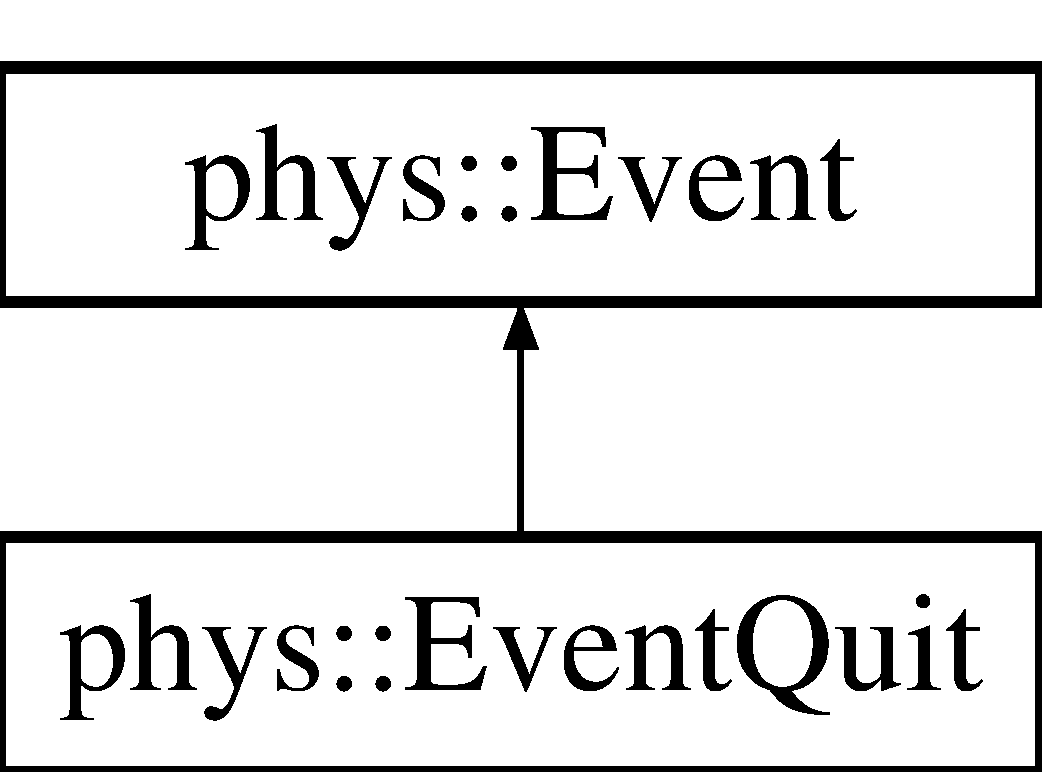
\includegraphics[height=2cm]{dd/dea/classphys_1_1EventQuit}
\end{center}
\end{figure}
\subsection*{Public Member Functions}
\begin{DoxyCompactItemize}
\item 
virtual \hyperlink{classphys_1_1EventBase_a5e6a8564e127f654123f0bf6a2751923}{EventType} \hyperlink{classphys_1_1EventQuit_a3bfca875349e73dbda47c3c62a253e3b}{GetType} () const 
\begin{DoxyCompactList}\small\item\em \hyperlink{structThis}{This} returns EventType::QuitMessage. \item\end{DoxyCompactList}\end{DoxyCompactItemize}


\subsection{Detailed Description}
\hyperlink{structThis}{This} is intended to convey the message that quitting needs to happen. \hyperlink{structThis}{This} stores not data other than the fact that this is a Quit event. \hyperlink{structThis}{This} means that either an underlying system like the OS or a service has requested a quit, or the application has manually put a quit message in the queue to signal that a graceful shutdown needs to occur. 

Definition at line 61 of file eventquit.h.



\subsection{Member Function Documentation}
\hypertarget{classphys_1_1EventQuit_a3bfca875349e73dbda47c3c62a253e3b}{
\index{phys::EventQuit@{phys::EventQuit}!GetType@{GetType}}
\index{GetType@{GetType}!phys::EventQuit@{phys::EventQuit}}
\subsubsection[{GetType}]{\setlength{\rightskip}{0pt plus 5cm}{\bf EventBase::EventType} phys::EventQuit::GetType () const\hspace{0.3cm}{\ttfamily  \mbox{[}virtual\mbox{]}}}}
\label{dd/dea/classphys_1_1EventQuit_a3bfca875349e73dbda47c3c62a253e3b}


\hyperlink{structThis}{This} returns EventType::QuitMessage. 

\hyperlink{structThis}{This} returns the kind of message this is, specifcally EventType::QuitMessage . If this functions returns EventType::QuitMessage, then and event pointer can safely be cast to \hyperlink{classphys_1_1EventQuit}{phys::EventQuit} . \hyperlink{structThis}{This} method is inherited from phys::Event . 

Implements \hyperlink{classphys_1_1EventBase_a1b3d29b6ecf30f18cc3e1825a515c508}{phys::EventBase}.



Definition at line 48 of file eventquit.cpp.



The documentation for this class was generated from the following files:\begin{DoxyCompactItemize}
\item 
eventquit.h\item 
eventquit.cpp\end{DoxyCompactItemize}

\hypertarget{classphys_1_1EventRenderTime}{
\section{phys::EventRenderTime Class Reference}
\label{d3/d8b/classphys_1_1EventRenderTime}\index{phys::EventRenderTime@{phys::EventRenderTime}}
}


This communicates the amount of time since the world was rendered.  




{\ttfamily \#include $<$eventrendertime.h$>$}

Inheritance diagram for phys::EventRenderTime:\begin{figure}[H]
\begin{center}
\leavevmode
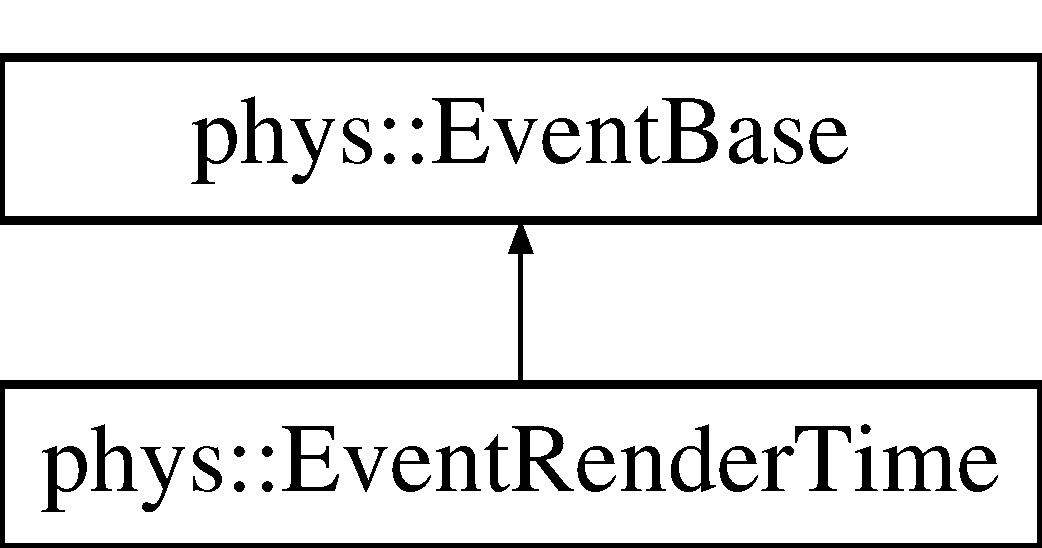
\includegraphics[height=2cm]{d3/d8b/classphys_1_1EventRenderTime}
\end{center}
\end{figure}
\subsection*{Public Member Functions}
\begin{DoxyCompactItemize}
\item 
\hyperlink{classphys_1_1EventRenderTime_af2384f7b09bbea42dcd2539a9e1747fd}{EventRenderTime} (Whole Milliseconds)
\begin{DoxyCompactList}\small\item\em The Constructor. \item\end{DoxyCompactList}\item 
virtual \hyperlink{classphys_1_1EventBase_a5e6a8564e127f654123f0bf6a2751923}{EventType} \hyperlink{classphys_1_1EventRenderTime_a76a47983d5aa197104cc3c0b9dea9dfa}{getEventType} () const 
\begin{DoxyCompactList}\small\item\em Returns that this event is a EventType::RenderTime. \item\end{DoxyCompactList}\item 
Whole \hyperlink{classphys_1_1EventRenderTime_ac9f20f13bf1f6e542151be2ce8ea2fa4}{getMilliSecondsSinceLastFrame} ()
\begin{DoxyCompactList}\small\item\em Returns the a floating point value with the amount of time. \item\end{DoxyCompactList}\end{DoxyCompactItemize}


\subsection{Detailed Description}
This communicates the amount of time since the world was rendered. This stores in milliseconds the amount of time since the last rendering of the world. 

Definition at line 59 of file eventrendertime.h.



\subsection{Constructor \& Destructor Documentation}
\hypertarget{classphys_1_1EventRenderTime_af2384f7b09bbea42dcd2539a9e1747fd}{
\index{phys::EventRenderTime@{phys::EventRenderTime}!EventRenderTime@{EventRenderTime}}
\index{EventRenderTime@{EventRenderTime}!phys::EventRenderTime@{phys::EventRenderTime}}
\subsubsection[{EventRenderTime}]{\setlength{\rightskip}{0pt plus 5cm}phys::EventRenderTime::EventRenderTime (Whole {\em Milliseconds})}}
\label{d3/d8b/classphys_1_1EventRenderTime_af2384f7b09bbea42dcd2539a9e1747fd}


The Constructor. 

This is the only way to set the time 
\begin{DoxyParams}{Parameters}
\item[{\em Milliseconds}]As it says, the amount of milliseconds since the last rendering \end{DoxyParams}


Definition at line 53 of file eventrendertime.cpp.



\subsection{Member Function Documentation}
\hypertarget{classphys_1_1EventRenderTime_a76a47983d5aa197104cc3c0b9dea9dfa}{
\index{phys::EventRenderTime@{phys::EventRenderTime}!getEventType@{getEventType}}
\index{getEventType@{getEventType}!phys::EventRenderTime@{phys::EventRenderTime}}
\subsubsection[{getEventType}]{\setlength{\rightskip}{0pt plus 5cm}{\bf EventBase::EventType} phys::EventRenderTime::getEventType () const\hspace{0.3cm}{\ttfamily  \mbox{[}virtual\mbox{]}}}}
\label{d3/d8b/classphys_1_1EventRenderTime_a76a47983d5aa197104cc3c0b9dea9dfa}


Returns that this event is a EventType::RenderTime. 

This is primarily for the benefit of sorting thorugh event pointers. If this functions returns EventType::RenderTime, then and event pointer can safely be cast to \hyperlink{classphys_1_1EventRenderTime}{phys::EventRenderTime} . This method is inherited from phys::Event . 

Implements \hyperlink{classphys_1_1EventBase_a0f39a25f4b64f7cf701e174454616366}{phys::EventBase}.



Definition at line 58 of file eventrendertime.cpp.

\hypertarget{classphys_1_1EventRenderTime_ac9f20f13bf1f6e542151be2ce8ea2fa4}{
\index{phys::EventRenderTime@{phys::EventRenderTime}!getMilliSecondsSinceLastFrame@{getMilliSecondsSinceLastFrame}}
\index{getMilliSecondsSinceLastFrame@{getMilliSecondsSinceLastFrame}!phys::EventRenderTime@{phys::EventRenderTime}}
\subsubsection[{getMilliSecondsSinceLastFrame}]{\setlength{\rightskip}{0pt plus 5cm}Whole phys::EventRenderTime::getMilliSecondsSinceLastFrame ()}}
\label{d3/d8b/classphys_1_1EventRenderTime_ac9f20f13bf1f6e542151be2ce8ea2fa4}


Returns the a floating point value with the amount of time. 

Returns the a floating point value with the amount of time. \begin{DoxyReturn}{Returns}
A floating point value with the amount of time. 
\end{DoxyReturn}


Definition at line 63 of file eventrendertime.cpp.



The documentation for this class was generated from the following files:\begin{DoxyCompactItemize}
\item 
eventrendertime.h\item 
eventrendertime.cpp\end{DoxyCompactItemize}

\hypertarget{classphys_1_1GraphicsSettings}{
\section{phys::GraphicsSettings Class Reference}
\label{dc/df1/classphys_1_1GraphicsSettings}\index{phys::GraphicsSettings@{phys::GraphicsSettings}}
}


This is intended to store basic graphics setting for the user.  




{\ttfamily \#include $<$graphicsettings.h$>$}

\subsection*{Public Member Functions}
\begin{DoxyCompactItemize}
\item 
\hyperlink{classphys_1_1GraphicsSettings_aceaaf53585413067adbf271e2c1e48fa}{GraphicsSettings} ()
\begin{DoxyCompactList}\small\item\em Default constructor. \item\end{DoxyCompactList}\item 
\hyperlink{classphys_1_1GraphicsSettings_a7cbb84f41101ef66a04e2a0990f796a2}{GraphicsSettings} (const \hyperlink{namespacephys_a460f6bc24c8dd347b05e0366ae34f34a}{Whole} \&Width\_\-, const \hyperlink{namespacephys_a460f6bc24c8dd347b05e0366ae34f34a}{Whole} \&Height\_\-, const bool \&FullScreen\_\-)
\begin{DoxyCompactList}\small\item\em Versatile Constructor. \item\end{DoxyCompactList}\item 
void \hyperlink{classphys_1_1GraphicsSettings_a63d41a500ee1ddf0ea9ffba5e353bae0}{Construct} (const \hyperlink{namespacephys_a460f6bc24c8dd347b05e0366ae34f34a}{Whole} \&Width\_\-, const \hyperlink{namespacephys_a460f6bc24c8dd347b05e0366ae34f34a}{Whole} \&Height\_\-, const bool \&FullScreen\_\-)
\begin{DoxyCompactList}\small\item\em Adjust all Settings. \item\end{DoxyCompactList}\item 
bool \hyperlink{classphys_1_1GraphicsSettings_a8871ea7d5c65c3b59d1d34b59531743f}{getFullscreen} () const 
\begin{DoxyCompactList}\small\item\em Gets the Fullscreen Setting. \item\end{DoxyCompactList}\item 
void \hyperlink{classphys_1_1GraphicsSettings_aba9e127ab2cf3f20604313e39d32f7a8}{setFullscreen} (const bool \&Fullscreen\_\-)
\begin{DoxyCompactList}\small\item\em Set the Fullscreen Setting. \item\end{DoxyCompactList}\item 
\hyperlink{namespacephys_a460f6bc24c8dd347b05e0366ae34f34a}{Whole} \hyperlink{classphys_1_1GraphicsSettings_a118171db4fc0a2b17da4284cc91fbeb4}{getRenderHeight} () const 
\begin{DoxyCompactList}\small\item\em Gets the Height of the Rendering Area. \item\end{DoxyCompactList}\item 
void \hyperlink{classphys_1_1GraphicsSettings_a1e6b11740f681beb4d64553656a760f1}{setRenderHeight} (const \hyperlink{namespacephys_a460f6bc24c8dd347b05e0366ae34f34a}{Whole} \&Height\_\-)
\begin{DoxyCompactList}\small\item\em Sets the Height. \item\end{DoxyCompactList}\item 
\hyperlink{namespacephys_a460f6bc24c8dd347b05e0366ae34f34a}{Whole} \hyperlink{classphys_1_1GraphicsSettings_aa8a8548afca8d3e127a1be69a2c1eba2}{getRenderWidth} () const 
\begin{DoxyCompactList}\small\item\em Gets the Width of the Rendering Area. \item\end{DoxyCompactList}\item 
void \hyperlink{classphys_1_1GraphicsSettings_a7cebb39f829f5e600231b4efc22b9ec3}{setRenderWidth} (const \hyperlink{namespacephys_a460f6bc24c8dd347b05e0366ae34f34a}{Whole} \&Width\_\-)
\begin{DoxyCompactList}\small\item\em Sets the Width. \item\end{DoxyCompactList}\end{DoxyCompactItemize}


\subsection{Detailed Description}
This is intended to store basic graphics setting for the user. This stores x/y resolution, fullscreen and in the future other settings. This is intended to make it easy for developers to pass/move around complex graphics settings. We hope to eventually include other items like shader settings, rendering API, and maybe other settings too. 

Definition at line 53 of file graphicsettings.h.



\subsection{Constructor \& Destructor Documentation}
\hypertarget{classphys_1_1GraphicsSettings_aceaaf53585413067adbf271e2c1e48fa}{
\index{phys::GraphicsSettings@{phys::GraphicsSettings}!GraphicsSettings@{GraphicsSettings}}
\index{GraphicsSettings@{GraphicsSettings}!phys::GraphicsSettings@{phys::GraphicsSettings}}
\subsubsection[{GraphicsSettings}]{\setlength{\rightskip}{0pt plus 5cm}phys::GraphicsSettings::GraphicsSettings ()}}
\label{dc/df1/classphys_1_1GraphicsSettings_aceaaf53585413067adbf271e2c1e48fa}


Default constructor. 

This creates a default Graphics Settings with resolution 640x480 with fullscreen set to false 

Definition at line 51 of file graphicsettings.cpp.

\hypertarget{classphys_1_1GraphicsSettings_a7cbb84f41101ef66a04e2a0990f796a2}{
\index{phys::GraphicsSettings@{phys::GraphicsSettings}!GraphicsSettings@{GraphicsSettings}}
\index{GraphicsSettings@{GraphicsSettings}!phys::GraphicsSettings@{phys::GraphicsSettings}}
\subsubsection[{GraphicsSettings}]{\setlength{\rightskip}{0pt plus 5cm}phys::GraphicsSettings::GraphicsSettings (const {\bf Whole} \& {\em Width\_\-}, \/  const {\bf Whole} \& {\em Height\_\-}, \/  const bool \& {\em FullScreen\_\-})}}
\label{dc/df1/classphys_1_1GraphicsSettings_a7cbb84f41101ef66a04e2a0990f796a2}


Versatile Constructor. 


\begin{DoxyParams}{Parameters}
\item[{\em Width\_\-}]The desired width. \item[{\em Height\_\-}]The desired height. \item[{\em FullScreen\_\-}]True if fullscreen, false if not.\end{DoxyParams}
This creates a Graphics Settings with resolution and fullscreen passed into to it. Be careful that the settings selected are appropriate. Many mobile devices do not support windows, and many screens do not support arbitrary resolutions in fullscreen mode. 

Definition at line 56 of file graphicsettings.cpp.



\subsection{Member Function Documentation}
\hypertarget{classphys_1_1GraphicsSettings_a63d41a500ee1ddf0ea9ffba5e353bae0}{
\index{phys::GraphicsSettings@{phys::GraphicsSettings}!Construct@{Construct}}
\index{Construct@{Construct}!phys::GraphicsSettings@{phys::GraphicsSettings}}
\subsubsection[{Construct}]{\setlength{\rightskip}{0pt plus 5cm}void phys::GraphicsSettings::Construct (const {\bf Whole} \& {\em Width\_\-}, \/  const {\bf Whole} \& {\em Height\_\-}, \/  const bool \& {\em FullScreen\_\-})}}
\label{dc/df1/classphys_1_1GraphicsSettings_a63d41a500ee1ddf0ea9ffba5e353bae0}


Adjust all Settings. 


\begin{DoxyParams}{Parameters}
\item[{\em Width\_\-}]The desired width. \item[{\em Height\_\-}]The desired height. \item[{\em FullScreen\_\-}]True if fullscreen, false if not.\end{DoxyParams}
This adjusts most data in this Graphics Settings and accepts new resolution and fullscreen settings. Be careful that the settings selected are appropriate. Many mobile devices do not support windows, and many screens do not support arbitrary resolutions in fullscreen mode. 

Definition at line 61 of file graphicsettings.cpp.

\hypertarget{classphys_1_1GraphicsSettings_a8871ea7d5c65c3b59d1d34b59531743f}{
\index{phys::GraphicsSettings@{phys::GraphicsSettings}!getFullscreen@{getFullscreen}}
\index{getFullscreen@{getFullscreen}!phys::GraphicsSettings@{phys::GraphicsSettings}}
\subsubsection[{getFullscreen}]{\setlength{\rightskip}{0pt plus 5cm}bool phys::GraphicsSettings::getFullscreen () const}}
\label{dc/df1/classphys_1_1GraphicsSettings_a8871ea7d5c65c3b59d1d34b59531743f}


Gets the Fullscreen Setting. 

Gets the Fullscreen Setting \begin{DoxyReturn}{Returns}
This returns a bool, true if fullscreen is set, false otherwise 
\end{DoxyReturn}


Definition at line 72 of file graphicsettings.cpp.

\hypertarget{classphys_1_1GraphicsSettings_a118171db4fc0a2b17da4284cc91fbeb4}{
\index{phys::GraphicsSettings@{phys::GraphicsSettings}!getRenderHeight@{getRenderHeight}}
\index{getRenderHeight@{getRenderHeight}!phys::GraphicsSettings@{phys::GraphicsSettings}}
\subsubsection[{getRenderHeight}]{\setlength{\rightskip}{0pt plus 5cm}{\bf Whole} phys::GraphicsSettings::getRenderHeight () const}}
\label{dc/df1/classphys_1_1GraphicsSettings_a118171db4fc0a2b17da4284cc91fbeb4}


Gets the Height of the Rendering Area. 

Gets the Height of the Rendering Area \begin{DoxyReturn}{Returns}
This returns the Height of the Rendering Area 
\end{DoxyReturn}


Definition at line 87 of file graphicsettings.cpp.

\hypertarget{classphys_1_1GraphicsSettings_aa8a8548afca8d3e127a1be69a2c1eba2}{
\index{phys::GraphicsSettings@{phys::GraphicsSettings}!getRenderWidth@{getRenderWidth}}
\index{getRenderWidth@{getRenderWidth}!phys::GraphicsSettings@{phys::GraphicsSettings}}
\subsubsection[{getRenderWidth}]{\setlength{\rightskip}{0pt plus 5cm}{\bf Whole} phys::GraphicsSettings::getRenderWidth () const}}
\label{dc/df1/classphys_1_1GraphicsSettings_aa8a8548afca8d3e127a1be69a2c1eba2}


Gets the Width of the Rendering Area. 

Gets the Width of the Rendering Area \begin{DoxyReturn}{Returns}
This returns the Width of the Rendering Area 
\end{DoxyReturn}


Definition at line 92 of file graphicsettings.cpp.

\hypertarget{classphys_1_1GraphicsSettings_aba9e127ab2cf3f20604313e39d32f7a8}{
\index{phys::GraphicsSettings@{phys::GraphicsSettings}!setFullscreen@{setFullscreen}}
\index{setFullscreen@{setFullscreen}!phys::GraphicsSettings@{phys::GraphicsSettings}}
\subsubsection[{setFullscreen}]{\setlength{\rightskip}{0pt plus 5cm}void phys::GraphicsSettings::setFullscreen (const bool \& {\em Fullscreen\_\-})}}
\label{dc/df1/classphys_1_1GraphicsSettings_aba9e127ab2cf3f20604313e39d32f7a8}


Set the Fullscreen Setting. 

Set the Fullscreen Setting 
\begin{DoxyParams}{Parameters}
\item[{\em Fullscreen\_\-}]This accepts a bool. True for fullscreen, false for windowed \end{DoxyParams}


\begin{Desc}
\item[\hyperlink{todo__todo000007}{Todo}]TODO: We really should double check that going into fullscreen worked the way we wanted, this fails in too many games \end{Desc}




Definition at line 78 of file graphicsettings.cpp.

\hypertarget{classphys_1_1GraphicsSettings_a1e6b11740f681beb4d64553656a760f1}{
\index{phys::GraphicsSettings@{phys::GraphicsSettings}!setRenderHeight@{setRenderHeight}}
\index{setRenderHeight@{setRenderHeight}!phys::GraphicsSettings@{phys::GraphicsSettings}}
\subsubsection[{setRenderHeight}]{\setlength{\rightskip}{0pt plus 5cm}void phys::GraphicsSettings::setRenderHeight (const {\bf Whole} \& {\em Height\_\-})}}
\label{dc/df1/classphys_1_1GraphicsSettings_a1e6b11740f681beb4d64553656a760f1}


Sets the Height. 

Set the Render Height inside the window in windowed mode, set the resolution of the screen in fullscreen 
\begin{DoxyParams}{Parameters}
\item[{\em Height\_\-}]This accepts a Whole. \end{DoxyParams}


Definition at line 97 of file graphicsettings.cpp.

\hypertarget{classphys_1_1GraphicsSettings_a7cebb39f829f5e600231b4efc22b9ec3}{
\index{phys::GraphicsSettings@{phys::GraphicsSettings}!setRenderWidth@{setRenderWidth}}
\index{setRenderWidth@{setRenderWidth}!phys::GraphicsSettings@{phys::GraphicsSettings}}
\subsubsection[{setRenderWidth}]{\setlength{\rightskip}{0pt plus 5cm}void phys::GraphicsSettings::setRenderWidth (const {\bf Whole} \& {\em Width\_\-})}}
\label{dc/df1/classphys_1_1GraphicsSettings_a7cebb39f829f5e600231b4efc22b9ec3}


Sets the Width. 

Set the Render Width inside the window in windowed mode, set the resolution of the screen in fullscreen 
\begin{DoxyParams}{Parameters}
\item[{\em Width\_\-}]This accepts a Whole. \end{DoxyParams}


Definition at line 102 of file graphicsettings.cpp.



The documentation for this class was generated from the following files:\begin{DoxyCompactItemize}
\item 
graphicsettings.h\item 
graphicsettings.cpp\end{DoxyCompactItemize}

\hypertarget{classphys_1_1debug_1_1InternalDebugDrawer}{
\section{phys::debug::InternalDebugDrawer Class Reference}
\label{db/d27/classphys_1_1debug_1_1InternalDebugDrawer}\index{phys::debug::InternalDebugDrawer@{phys::debug::InternalDebugDrawer}}
}


This is used to draw wireframse for the Physics subsystem.  


\subsection*{Public Member Functions}
\begin{DoxyCompactItemize}
\item 
\hypertarget{classphys_1_1debug_1_1InternalDebugDrawer_a2bdb7e9da99e2d0cd2796cf9c67c3456}{
{\bfseries InternalDebugDrawer} (\hyperlink{classphys_1_1World}{phys::World} $\ast$ParentWorld\_\-, \hyperlink{namespacephys_a460f6bc24c8dd347b05e0366ae34f34a}{Whole} WireFrameCount\_\-=1)}
\label{db/d27/classphys_1_1debug_1_1InternalDebugDrawer_a2bdb7e9da99e2d0cd2796cf9c67c3456}

\item 
\hypertarget{classphys_1_1debug_1_1InternalDebugDrawer_a8a35c3c80fddaaec8e21f737ed1b3938}{
virtual void {\bfseries drawLine} (const btVector3 \&from, const btVector3 \&to, const btVector3 \&color)}
\label{db/d27/classphys_1_1debug_1_1InternalDebugDrawer_a8a35c3c80fddaaec8e21f737ed1b3938}

\item 
\hypertarget{classphys_1_1debug_1_1InternalDebugDrawer_a8b912aaff8dfd9f4e97ffb2d867121b2}{
virtual void {\bfseries drawContactPoint} (const btVector3 \&PointOnB, const btVector3 \&normalOnB, btScalar distance, int lifeTime, const btVector3 \&color)}
\label{db/d27/classphys_1_1debug_1_1InternalDebugDrawer_a8b912aaff8dfd9f4e97ffb2d867121b2}

\item 
\hypertarget{classphys_1_1debug_1_1InternalDebugDrawer_a4e3b4cbc861f76696b4d32f0cf068ea6}{
virtual void {\bfseries reportErrorWarning} (const char $\ast$warningString)}
\label{db/d27/classphys_1_1debug_1_1InternalDebugDrawer_a4e3b4cbc861f76696b4d32f0cf068ea6}

\item 
\hypertarget{classphys_1_1debug_1_1InternalDebugDrawer_a1266d3fad8868ade2d515e9c92e76b4a}{
virtual void {\bfseries draw3dText} (const btVector3 \&location, const char $\ast$textString)}
\label{db/d27/classphys_1_1debug_1_1InternalDebugDrawer_a1266d3fad8868ade2d515e9c92e76b4a}

\item 
\hypertarget{classphys_1_1debug_1_1InternalDebugDrawer_a63059b273ed6031a393b2d994b820bcc}{
virtual void {\bfseries setDebugMode} (int debugMode)}
\label{db/d27/classphys_1_1debug_1_1InternalDebugDrawer_a63059b273ed6031a393b2d994b820bcc}

\item 
\hypertarget{classphys_1_1debug_1_1InternalDebugDrawer_aba329861569d741e970ce5aafb668e84}{
virtual int {\bfseries getDebugMode} () const }
\label{db/d27/classphys_1_1debug_1_1InternalDebugDrawer_aba329861569d741e970ce5aafb668e84}

\item 
\hypertarget{classphys_1_1debug_1_1InternalDebugDrawer_aa1666e636e6ff81813c0b1a85d7bc157}{
virtual \hyperlink{namespacephys_a460f6bc24c8dd347b05e0366ae34f34a}{Whole} {\bfseries GetWireFrameCount} ()}
\label{db/d27/classphys_1_1debug_1_1InternalDebugDrawer_aa1666e636e6ff81813c0b1a85d7bc157}

\item 
\hypertarget{classphys_1_1debug_1_1InternalDebugDrawer_a76922fda7bb3b59d301e50d67e4f3c72}{
virtual void {\bfseries SetWireFrameCount} (\hyperlink{namespacephys_a460f6bc24c8dd347b05e0366ae34f34a}{Whole} WireFrameCount\_\-)}
\label{db/d27/classphys_1_1debug_1_1InternalDebugDrawer_a76922fda7bb3b59d301e50d67e4f3c72}

\end{DoxyCompactItemize}


\subsection{Detailed Description}
This is used to draw wireframse for the Physics subsystem. \begin{DoxyInternal}{For internal use only.}
\end{DoxyInternal}


Definition at line 86 of file world.cpp.



The documentation for this class was generated from the following file:\begin{DoxyCompactItemize}
\item 
world.cpp\end{DoxyCompactItemize}

\hypertarget{classphys_1_1debug_1_1Line3D}{
\section{phys::debug::Line3D Class Reference}
\label{d6/d1b/classphys_1_1debug_1_1Line3D}\index{phys::debug::Line3D@{phys::debug::Line3D}}
}
\subsection*{Public Member Functions}
\begin{DoxyCompactItemize}
\item 
\hypertarget{classphys_1_1debug_1_1Line3D_a449ea187f5bbf16f73f4d8dc7977addb}{
void {\bfseries addPoint} (const Vector3 \&p)}
\label{d6/d1b/classphys_1_1debug_1_1Line3D_a449ea187f5bbf16f73f4d8dc7977addb}

\item 
\hypertarget{classphys_1_1debug_1_1Line3D_a7c275f3f7c48d7a7ad807bd419547d45}{
const Vector3 \& {\bfseries getPoint} (unsigned short index) const }
\label{d6/d1b/classphys_1_1debug_1_1Line3D_a7c275f3f7c48d7a7ad807bd419547d45}

\item 
\hypertarget{classphys_1_1debug_1_1Line3D_ad10a08d99077ac3ac5c68e3b1c121805}{
unsigned short {\bfseries getNumPoints} (void) const }
\label{d6/d1b/classphys_1_1debug_1_1Line3D_ad10a08d99077ac3ac5c68e3b1c121805}

\item 
\hypertarget{classphys_1_1debug_1_1Line3D_a9f12d620c63df9bbffbd68d3a73317a1}{
void {\bfseries updatePoint} (unsigned short index, const Vector3 \&value)}
\label{d6/d1b/classphys_1_1debug_1_1Line3D_a9f12d620c63df9bbffbd68d3a73317a1}

\item 
\hypertarget{classphys_1_1debug_1_1Line3D_ad0d6ed90fbbff7e9d568c2c773a202f3}{
void {\bfseries drawLine} (Vector3 \&start, Vector3 \&end)}
\label{d6/d1b/classphys_1_1debug_1_1Line3D_ad0d6ed90fbbff7e9d568c2c773a202f3}

\item 
\hypertarget{classphys_1_1debug_1_1Line3D_afb66ce45cef0dfca3f79056b5bf36318}{
void {\bfseries drawLines} (void)}
\label{d6/d1b/classphys_1_1debug_1_1Line3D_afb66ce45cef0dfca3f79056b5bf36318}

\item 
\hypertarget{classphys_1_1debug_1_1Line3D_ae8ad277bea57629e860acce0d14a0643}{
\hyperlink{namespacephys_af7eb897198d265b8e868f45240230d5f}{Real} {\bfseries getSquaredViewDepth} (const Camera $\ast$cam) const }
\label{d6/d1b/classphys_1_1debug_1_1Line3D_ae8ad277bea57629e860acce0d14a0643}

\item 
\hypertarget{classphys_1_1debug_1_1Line3D_ad67db03f607f3544c1f3726d0c160bbb}{
\hyperlink{namespacephys_af7eb897198d265b8e868f45240230d5f}{Real} {\bfseries getBoundingRadius} (void) const }
\label{d6/d1b/classphys_1_1debug_1_1Line3D_ad67db03f607f3544c1f3726d0c160bbb}

\end{DoxyCompactItemize}
\subsection*{Protected Member Functions}
\begin{DoxyCompactItemize}
\item 
\hypertarget{classphys_1_1debug_1_1Line3D_a918d57f174432e6cbf4b31282b2140da}{
const Ogre::Quaternion \& {\bfseries getWorldOrientation} (void) const }
\label{d6/d1b/classphys_1_1debug_1_1Line3D_a918d57f174432e6cbf4b31282b2140da}

\item 
\hypertarget{classphys_1_1debug_1_1Line3D_a2cf807b1c4d3770889ba8e5114619d4b}{
const Vector3 \& {\bfseries getWorldPosition} (void) const }
\label{d6/d1b/classphys_1_1debug_1_1Line3D_a2cf807b1c4d3770889ba8e5114619d4b}

\end{DoxyCompactItemize}
\subsection*{Protected Attributes}
\begin{DoxyCompactItemize}
\item 
\hypertarget{classphys_1_1debug_1_1Line3D_ad82efc7c9d8cd1ca573c956705316807}{
std::vector$<$ Vector3 $>$ {\bfseries mPoints}}
\label{d6/d1b/classphys_1_1debug_1_1Line3D_ad82efc7c9d8cd1ca573c956705316807}

\item 
\hypertarget{classphys_1_1debug_1_1Line3D_a70e1784bd640ae3a3b9b755a40bc9185}{
bool {\bfseries mDrawn}}
\label{d6/d1b/classphys_1_1debug_1_1Line3D_a70e1784bd640ae3a3b9b755a40bc9185}

\end{DoxyCompactItemize}


\subsection{Detailed Description}


Definition at line 108 of file world.cpp.



The documentation for this class was generated from the following file:\begin{DoxyCompactItemize}
\item 
world.cpp\end{DoxyCompactItemize}

\hypertarget{classphys_1_1MetaCode}{
\section{phys::MetaCode Class Reference}
\label{da/dc9/classphys_1_1MetaCode}\index{phys::MetaCode@{phys::MetaCode}}
}


This Determines the kind of user input.  




{\ttfamily \#include $<$metacode.h$>$}

\subsection*{Public Types}
\begin{DoxyCompactItemize}
\item 
enum \hyperlink{classphys_1_1MetaCode_a3e501cbb5bf0f6f1fdb7211465bda8d8}{InputCode} \{ \par
\hyperlink{classphys_1_1MetaCode_a3e501cbb5bf0f6f1fdb7211465bda8d8a061a36c9b5d9661314fd9d276b33042f}{KEY\_\-UNKNOWN} =  0, 
\hyperlink{classphys_1_1MetaCode_a3e501cbb5bf0f6f1fdb7211465bda8d8a45d7f3824a440f5bea5e616a6d6ea0b5}{KEY\_\-FIRST} =  0, 
{\bfseries KEY\_\-BACKSPACE} =  8, 
{\bfseries KEY\_\-TAB} =  9, 
\par
{\bfseries KEY\_\-CLEAR} =  12, 
{\bfseries KEY\_\-RETURN} =  13, 
{\bfseries KEY\_\-PAUSE} =  19, 
{\bfseries KEY\_\-ESCAPE} =  27, 
\par
{\bfseries KEY\_\-SPACE} =  32, 
{\bfseries KEY\_\-EXCLAIM} =  33, 
{\bfseries KEY\_\-QUOTEDBL} =  34, 
{\bfseries KEY\_\-HASH} =  35, 
\par
{\bfseries KEY\_\-DOLLAR} =  36, 
{\bfseries KEY\_\-AMPERSAND} =  38, 
{\bfseries KEY\_\-QUOTE} =  39, 
{\bfseries KEY\_\-LEFTPAREN} =  40, 
\par
{\bfseries KEY\_\-RIGHTPAREN} =  41, 
{\bfseries KEY\_\-ASTERISK} =  42, 
{\bfseries KEY\_\-PLUS} =  43, 
{\bfseries KEY\_\-COMMA} =  44, 
\par
{\bfseries KEY\_\-MINUS} =  45, 
{\bfseries KEY\_\-PERIOD} =  46, 
{\bfseries KEY\_\-SLASH} =  47, 
{\bfseries KEY\_\-0} =  48, 
\par
{\bfseries KEY\_\-1} =  49, 
{\bfseries KEY\_\-2} =  50, 
{\bfseries KEY\_\-3} =  51, 
{\bfseries KEY\_\-4} =  52, 
\par
{\bfseries KEY\_\-5} =  53, 
{\bfseries KEY\_\-6} =  54, 
{\bfseries KEY\_\-7} =  55, 
{\bfseries KEY\_\-8} =  56, 
\par
{\bfseries KEY\_\-9} =  57, 
{\bfseries KEY\_\-COLON} =  58, 
{\bfseries KEY\_\-SEMICOLON} =  59, 
{\bfseries KEY\_\-LESS} =  60, 
\par
{\bfseries KEY\_\-EQUALS} =  61, 
{\bfseries KEY\_\-GREATER} =  62, 
{\bfseries KEY\_\-QUESTION} =  63, 
{\bfseries KEY\_\-AT} =  64, 
\par
{\bfseries KEY\_\-LEFTBRACKET} =  91, 
{\bfseries KEY\_\-BACKSLASH} =  92, 
{\bfseries KEY\_\-RIGHTBRACKET} =  93, 
{\bfseries KEY\_\-CARET} =  94, 
\par
{\bfseries KEY\_\-UNDERSCORE} =  95, 
{\bfseries KEY\_\-BACKQUOTE} =  96, 
{\bfseries KEY\_\-a} =  97, 
{\bfseries KEY\_\-b} =  98, 
\par
{\bfseries KEY\_\-c} =  99, 
{\bfseries KEY\_\-d} =  100, 
{\bfseries KEY\_\-e} =  101, 
{\bfseries KEY\_\-f} =  102, 
\par
{\bfseries KEY\_\-g} =  103, 
{\bfseries KEY\_\-h} =  104, 
{\bfseries KEY\_\-i} =  105, 
{\bfseries KEY\_\-j} =  106, 
\par
{\bfseries KEY\_\-k} =  107, 
{\bfseries KEY\_\-l} =  108, 
{\bfseries KEY\_\-m} =  109, 
{\bfseries KEY\_\-n} =  110, 
\par
{\bfseries KEY\_\-o} =  111, 
{\bfseries KEY\_\-p} =  112, 
{\bfseries KEY\_\-q} =  113, 
{\bfseries KEY\_\-r} =  114, 
\par
{\bfseries KEY\_\-s} =  115, 
{\bfseries KEY\_\-t} =  116, 
{\bfseries KEY\_\-u} =  117, 
{\bfseries KEY\_\-v} =  118, 
\par
{\bfseries KEY\_\-w} =  119, 
{\bfseries KEY\_\-x} =  120, 
{\bfseries KEY\_\-y} =  121, 
{\bfseries KEY\_\-z} =  122, 
\par
{\bfseries KEY\_\-DELETE} =  127, 
{\bfseries KEY\_\-WORLD\_\-0} =  160, 
{\bfseries KEY\_\-WORLD\_\-1} =  161, 
{\bfseries KEY\_\-WORLD\_\-2} =  162, 
\par
{\bfseries KEY\_\-WORLD\_\-3} =  163, 
{\bfseries KEY\_\-WORLD\_\-4} =  164, 
{\bfseries KEY\_\-WORLD\_\-5} =  165, 
{\bfseries KEY\_\-WORLD\_\-6} =  166, 
\par
{\bfseries KEY\_\-WORLD\_\-7} =  167, 
{\bfseries KEY\_\-WORLD\_\-8} =  168, 
{\bfseries KEY\_\-WORLD\_\-9} =  169, 
{\bfseries KEY\_\-WORLD\_\-10} =  170, 
\par
{\bfseries KEY\_\-WORLD\_\-11} =  171, 
{\bfseries KEY\_\-WORLD\_\-12} =  172, 
{\bfseries KEY\_\-WORLD\_\-13} =  173, 
{\bfseries KEY\_\-WORLD\_\-14} =  174, 
\par
{\bfseries KEY\_\-WORLD\_\-15} =  175, 
{\bfseries KEY\_\-WORLD\_\-16} =  176, 
{\bfseries KEY\_\-WORLD\_\-17} =  177, 
{\bfseries KEY\_\-WORLD\_\-18} =  178, 
\par
{\bfseries KEY\_\-WORLD\_\-19} =  179, 
{\bfseries KEY\_\-WORLD\_\-20} =  180, 
{\bfseries KEY\_\-WORLD\_\-21} =  181, 
{\bfseries KEY\_\-WORLD\_\-22} =  182, 
\par
{\bfseries KEY\_\-WORLD\_\-23} =  183, 
{\bfseries KEY\_\-WORLD\_\-24} =  184, 
{\bfseries KEY\_\-WORLD\_\-25} =  185, 
{\bfseries KEY\_\-WORLD\_\-26} =  186, 
\par
{\bfseries KEY\_\-WORLD\_\-27} =  187, 
{\bfseries KEY\_\-WORLD\_\-28} =  188, 
{\bfseries KEY\_\-WORLD\_\-29} =  189, 
{\bfseries KEY\_\-WORLD\_\-30} =  190, 
\par
{\bfseries KEY\_\-WORLD\_\-31} =  191, 
{\bfseries KEY\_\-WORLD\_\-32} =  192, 
{\bfseries KEY\_\-WORLD\_\-33} =  193, 
{\bfseries KEY\_\-WORLD\_\-34} =  194, 
\par
{\bfseries KEY\_\-WORLD\_\-35} =  195, 
{\bfseries KEY\_\-WORLD\_\-36} =  196, 
{\bfseries KEY\_\-WORLD\_\-37} =  197, 
{\bfseries KEY\_\-WORLD\_\-38} =  198, 
\par
{\bfseries KEY\_\-WORLD\_\-39} =  199, 
{\bfseries KEY\_\-WORLD\_\-40} =  200, 
{\bfseries KEY\_\-WORLD\_\-41} =  201, 
{\bfseries KEY\_\-WORLD\_\-42} =  202, 
\par
{\bfseries KEY\_\-WORLD\_\-43} =  203, 
{\bfseries KEY\_\-WORLD\_\-44} =  204, 
{\bfseries KEY\_\-WORLD\_\-45} =  205, 
{\bfseries KEY\_\-WORLD\_\-46} =  206, 
\par
{\bfseries KEY\_\-WORLD\_\-47} =  207, 
{\bfseries KEY\_\-WORLD\_\-48} =  208, 
{\bfseries KEY\_\-WORLD\_\-49} =  209, 
{\bfseries KEY\_\-WORLD\_\-50} =  210, 
\par
{\bfseries KEY\_\-WORLD\_\-51} =  211, 
{\bfseries KEY\_\-WORLD\_\-52} =  212, 
{\bfseries KEY\_\-WORLD\_\-53} =  213, 
{\bfseries KEY\_\-WORLD\_\-54} =  214, 
\par
{\bfseries KEY\_\-WORLD\_\-55} =  215, 
{\bfseries KEY\_\-WORLD\_\-56} =  216, 
{\bfseries KEY\_\-WORLD\_\-57} =  217, 
{\bfseries KEY\_\-WORLD\_\-58} =  218, 
\par
{\bfseries KEY\_\-WORLD\_\-59} =  219, 
{\bfseries KEY\_\-WORLD\_\-60} =  220, 
{\bfseries KEY\_\-WORLD\_\-61} =  221, 
{\bfseries KEY\_\-WORLD\_\-62} =  222, 
\par
{\bfseries KEY\_\-WORLD\_\-63} =  223, 
{\bfseries KEY\_\-WORLD\_\-64} =  224, 
{\bfseries KEY\_\-WORLD\_\-65} =  225, 
{\bfseries KEY\_\-WORLD\_\-66} =  226, 
\par
{\bfseries KEY\_\-WORLD\_\-67} =  227, 
{\bfseries KEY\_\-WORLD\_\-68} =  228, 
{\bfseries KEY\_\-WORLD\_\-69} =  229, 
{\bfseries KEY\_\-WORLD\_\-70} =  230, 
\par
{\bfseries KEY\_\-WORLD\_\-71} =  231, 
{\bfseries KEY\_\-WORLD\_\-72} =  232, 
{\bfseries KEY\_\-WORLD\_\-73} =  233, 
{\bfseries KEY\_\-WORLD\_\-74} =  234, 
\par
{\bfseries KEY\_\-WORLD\_\-75} =  235, 
{\bfseries KEY\_\-WORLD\_\-76} =  236, 
{\bfseries KEY\_\-WORLD\_\-77} =  237, 
{\bfseries KEY\_\-WORLD\_\-78} =  238, 
\par
{\bfseries KEY\_\-WORLD\_\-79} =  239, 
{\bfseries KEY\_\-WORLD\_\-80} =  240, 
{\bfseries KEY\_\-WORLD\_\-81} =  241, 
{\bfseries KEY\_\-WORLD\_\-82} =  242, 
\par
{\bfseries KEY\_\-WORLD\_\-83} =  243, 
{\bfseries KEY\_\-WORLD\_\-84} =  244, 
{\bfseries KEY\_\-WORLD\_\-85} =  245, 
{\bfseries KEY\_\-WORLD\_\-86} =  246, 
\par
{\bfseries KEY\_\-WORLD\_\-87} =  247, 
{\bfseries KEY\_\-WORLD\_\-88} =  248, 
{\bfseries KEY\_\-WORLD\_\-89} =  249, 
{\bfseries KEY\_\-WORLD\_\-90} =  250, 
\par
{\bfseries KEY\_\-WORLD\_\-91} =  251, 
{\bfseries KEY\_\-WORLD\_\-92} =  252, 
{\bfseries KEY\_\-WORLD\_\-93} =  253, 
{\bfseries KEY\_\-WORLD\_\-94} =  254, 
\par
{\bfseries KEY\_\-WORLD\_\-95} =  255, 
{\bfseries KEY\_\-KP0} =  256, 
{\bfseries KEY\_\-KP1} =  257, 
{\bfseries KEY\_\-KP2} =  258, 
\par
{\bfseries KEY\_\-KP3} =  259, 
{\bfseries KEY\_\-KP4} =  260, 
{\bfseries KEY\_\-KP5} =  261, 
{\bfseries KEY\_\-KP6} =  262, 
\par
{\bfseries KEY\_\-KP7} =  263, 
{\bfseries KEY\_\-KP8} =  264, 
{\bfseries KEY\_\-KP9} =  265, 
{\bfseries KEY\_\-KP\_\-PERIOD} =  266, 
\par
{\bfseries KEY\_\-KP\_\-DIVIDE} =  267, 
{\bfseries KEY\_\-KP\_\-MULTIPLY} =  268, 
{\bfseries KEY\_\-KP\_\-MINUS} =  269, 
{\bfseries KEY\_\-KP\_\-PLUS} =  270, 
\par
{\bfseries KEY\_\-KP\_\-ENTER} =  271, 
{\bfseries KEY\_\-KP\_\-EQUALS} =  272, 
{\bfseries KEY\_\-UP} =  273, 
{\bfseries KEY\_\-DOWN} =  274, 
\par
{\bfseries KEY\_\-RIGHT} =  275, 
{\bfseries KEY\_\-LEFT} =  276, 
{\bfseries KEY\_\-INSERT} =  277, 
{\bfseries KEY\_\-HOME} =  278, 
\par
{\bfseries KEY\_\-END} =  279, 
{\bfseries KEY\_\-PAGEUP} =  280, 
{\bfseries KEY\_\-PAGEDOWN} =  281, 
{\bfseries KEY\_\-F1} =  282, 
\par
{\bfseries KEY\_\-F2} =  283, 
{\bfseries KEY\_\-F3} =  284, 
{\bfseries KEY\_\-F4} =  285, 
{\bfseries KEY\_\-F5} =  286, 
\par
{\bfseries KEY\_\-F6} =  287, 
{\bfseries KEY\_\-F7} =  288, 
{\bfseries KEY\_\-F8} =  289, 
{\bfseries KEY\_\-F9} =  290, 
\par
{\bfseries KEY\_\-F10} =  291, 
{\bfseries KEY\_\-F11} =  292, 
{\bfseries KEY\_\-F12} =  293, 
{\bfseries KEY\_\-F13} =  294, 
\par
{\bfseries KEY\_\-F14} =  295, 
{\bfseries KEY\_\-F15} =  296, 
{\bfseries KEY\_\-NUMLOCK} =  300, 
{\bfseries KEY\_\-CAPSLOCK} =  301, 
\par
{\bfseries KEY\_\-SCROLLOCK} =  302, 
{\bfseries KEY\_\-RSHIFT} =  303, 
{\bfseries KEY\_\-LSHIFT} =  304, 
{\bfseries KEY\_\-RCTRL} =  305, 
\par
{\bfseries KEY\_\-LCTRL} =  306, 
{\bfseries KEY\_\-RALT} =  307, 
{\bfseries KEY\_\-LALT} =  308, 
{\bfseries KEY\_\-RMETA} =  309, 
\par
{\bfseries KEY\_\-LMETA} =  310, 
\hyperlink{classphys_1_1MetaCode_a3e501cbb5bf0f6f1fdb7211465bda8d8aab77afaba4fc97faa9b9fe40d3a9ebbb}{KEY\_\-LSUPER} =  311, 
\hyperlink{classphys_1_1MetaCode_a3e501cbb5bf0f6f1fdb7211465bda8d8a84e2235ece031f83821867486ff52149}{KEY\_\-RSUPER} =  312, 
\hyperlink{classphys_1_1MetaCode_a3e501cbb5bf0f6f1fdb7211465bda8d8a9e26ea2006e876ccaa80fe4ae441da46}{KEY\_\-MODE} =  313, 
\par
\hyperlink{classphys_1_1MetaCode_a3e501cbb5bf0f6f1fdb7211465bda8d8aae92d5418d0273c8b43cb11f5e251a20}{KEY\_\-COMPOSE} =  314, 
{\bfseries KEY\_\-HELP} =  315, 
{\bfseries KEY\_\-PRINT} =  316, 
{\bfseries KEY\_\-SYSREQ} =  317, 
\par
{\bfseries KEY\_\-BREAK} =  318, 
{\bfseries KEY\_\-MENU} =  319, 
\hyperlink{classphys_1_1MetaCode_a3e501cbb5bf0f6f1fdb7211465bda8d8a08a2d04e3a40d746b81913e92a25a038}{KEY\_\-POWER} =  320, 
\hyperlink{classphys_1_1MetaCode_a3e501cbb5bf0f6f1fdb7211465bda8d8aee70075958d1650a7b48ba507103ec0c}{KEY\_\-EURO} =  321, 
\par
\hyperlink{classphys_1_1MetaCode_a3e501cbb5bf0f6f1fdb7211465bda8d8a15aabd8c4e36284ec057fafbda0d120a}{KEY\_\-UNDO} =  322, 
{\bfseries KEYMOD\_\-NONE} =  323, 
{\bfseries KEYMOD\_\-LSHIFT} =  324, 
{\bfseries KEYMOD\_\-RSHIFT} =  325, 
\par
{\bfseries KEYMOD\_\-LCTRL} =  326, 
{\bfseries KEYMOD\_\-RCTRL} =  327, 
{\bfseries KEYMOD\_\-LALT} =  328, 
{\bfseries KEYMOD\_\-RALT} =  329, 
\par
{\bfseries KEYMOD\_\-LMETA} =  330, 
{\bfseries KEYMOD\_\-RMETA} =  331, 
{\bfseries KEYMOD\_\-NUM} =  332, 
{\bfseries KEYMOD\_\-CAPS} =  333, 
\par
{\bfseries KEYMOD\_\-MODE} =  334, 
{\bfseries KEYMOD\_\-RESERVED} =  335, 
{\bfseries KEY\_\-LAST} =  379, 
\hyperlink{classphys_1_1MetaCode_a3e501cbb5bf0f6f1fdb7211465bda8d8a87685f9ca9462b329f2b86a17514f136}{INPUTEVENT\_\-FIRST} =  380, 
\par
\hyperlink{classphys_1_1MetaCode_a3e501cbb5bf0f6f1fdb7211465bda8d8a355649b334e903ada2496ad39dcd5f9d}{MOTION\_\-FIRST} =  460, 
\hyperlink{classphys_1_1MetaCode_a3e501cbb5bf0f6f1fdb7211465bda8d8a59cc92f5b2f42f7a138f8ea22e92d626}{MOTION\_\-LAST} =  469, 
\hyperlink{classphys_1_1MetaCode_a3e501cbb5bf0f6f1fdb7211465bda8d8acdb03d23d93022d5962db5026475b9c7}{MULTITOUCH\_\-FIRST} =  470, 
\hyperlink{classphys_1_1MetaCode_a3e501cbb5bf0f6f1fdb7211465bda8d8a94d804dc2330be620a8009252b5d5d22}{MULTITOUCH\_\-ACTION} =  471, 
\par
{\bfseries MULTITOUCH\_\-GESTURE} =  472, 
{\bfseries MULTITOUCH\_\-PINCH} =  473, 
{\bfseries MULTITOUCH\_\-STRETCH} =  474, 
{\bfseries MULTITOUCH\_\-LAST} =  479, 
\par
\hyperlink{classphys_1_1MetaCode_a3e501cbb5bf0f6f1fdb7211465bda8d8a1bb7f008c7d430e886141a3b8b697129}{MOUSE\_\-FIRST} =  480, 
\hyperlink{classphys_1_1MetaCode_a3e501cbb5bf0f6f1fdb7211465bda8d8a9cc80a2db206fb540fbb92a8ff64268a}{MOUSEBUTTON} =  481, 
{\bfseries MOUSEABSOLUTEVERTICAL} =  482, 
{\bfseries MOUSEABSOLUTEHORIZONTAL} =  483, 
\par
{\bfseries MOUSEVERTICAL} =  484, 
{\bfseries MOUSEHORIZONTAL} =  485, 
{\bfseries MOUSEWHEELVERTICAL} =  486, 
{\bfseries MOUSEWHEELHORIZONTAL} =  489, 
\par
{\bfseries MOUSE\_\-LAST} =  490, 
\hyperlink{classphys_1_1MetaCode_a3e501cbb5bf0f6f1fdb7211465bda8d8a666e564cae666de739b9b3cf047ec578}{JOYSTICK\_\-FIRST} =  499, 
\hyperlink{classphys_1_1MetaCode_a3e501cbb5bf0f6f1fdb7211465bda8d8aaaa2af6a60a9cd7403aa4786ef1ea389}{JOYSTICKBUTTON} =  500, 
{\bfseries JOYSTICKMOTIONAXIS} =  501, 
\par
{\bfseries JOYSTICKBALLVERTICAL} =  502, 
{\bfseries JOYSTICKBALLHORIZONTAL} =  503, 
{\bfseries JOYSTICKHATVERTICAL} =  504, 
{\bfseries JOYSTICKHATHORIZONTAL} =  505, 
\par
{\bfseries JOYSTICK\_\-LAST} =  506, 
\hyperlink{classphys_1_1MetaCode_a3e501cbb5bf0f6f1fdb7211465bda8d8adc78bfd04a85c4bbe39718f9acacbbe3}{INPUTEVENT\_\-LAST} =  512
 \}
\begin{DoxyCompactList}\small\item\em The InputCode enum defines all the posible types of inputs. \item\end{DoxyCompactList}\item 
enum \hyperlink{classphys_1_1MetaCode_a2fdfb26b3e50ceb0ccc60bfc4c3d6ac2}{ButtonState} \{ \hyperlink{classphys_1_1MetaCode_a2fdfb26b3e50ceb0ccc60bfc4c3d6ac2a6b5564408703517f36debd8c423e2dee}{BUTTON\_\-LIFTING} =  -\/1, 
\hyperlink{classphys_1_1MetaCode_a2fdfb26b3e50ceb0ccc60bfc4c3d6ac2ae275c52779b0f6ec37533af256a70cc3}{BUTTON\_\-UP} =  0, 
\hyperlink{classphys_1_1MetaCode_a2fdfb26b3e50ceb0ccc60bfc4c3d6ac2a33669b2b9ca814664296da55702e412d}{BUTTON\_\-PRESSING} =  1, 
\hyperlink{classphys_1_1MetaCode_a2fdfb26b3e50ceb0ccc60bfc4c3d6ac2a5b52ee1db94dbc2db23f3b4c267b5438}{BUTTON\_\-DOWN} =  2
 \}
\begin{DoxyCompactList}\small\item\em An Optional listing of value that can be used in a metacode to represent the information of a button press. \item\end{DoxyCompactList}\item 
enum \hyperlink{classphys_1_1MetaCode_af9ba277d1ef071be8861e35c2b7d82d6}{MouseWheelState} \{ \hyperlink{classphys_1_1MetaCode_af9ba277d1ef071be8861e35c2b7d82d6a15542262fc8fe9a3d6746f2b84ecde11}{MOUSEWHEEL\_\-UP} =  1, 
\hyperlink{classphys_1_1MetaCode_af9ba277d1ef071be8861e35c2b7d82d6aa3d86fe74d1c191d7c57f886c0b8d99a}{MOUSEWHEEL\_\-UNCHANGED} =  0, 
\hyperlink{classphys_1_1MetaCode_af9ba277d1ef071be8861e35c2b7d82d6ab6edd0886d2ec2d2917bbad96ce3d510}{MOUSEWHEEL\_\-DOWN} =  -\/1
 \}
\begin{DoxyCompactList}\small\item\em An Optional listing of values that can be used in a metacode Indicate spin of a mouse wheel. \item\end{DoxyCompactList}\end{DoxyCompactItemize}
\subsection*{Public Member Functions}
\begin{DoxyCompactItemize}
\item 
\hyperlink{classphys_1_1MetaCode_ae2c80c84f924ddfd880f46ffe6a1746e}{MetaCode} ()
\begin{DoxyCompactList}\small\item\em Default constructor. \item\end{DoxyCompactList}\item 
\hyperlink{classphys_1_1MetaCode_a05bcc50a09a9a5d19520dc258841f117}{MetaCode} (const int \&MetaValue\_\-, const short unsigned int \&ID\_\-, const \hyperlink{classphys_1_1MetaCode_a3e501cbb5bf0f6f1fdb7211465bda8d8}{MetaCode::InputCode} \&Code\_\-)
\begin{DoxyCompactList}\small\item\em Descriptive Constructor. \item\end{DoxyCompactList}\item 
\hyperlink{classphys_1_1MetaCode_ad9a618b5cc6f9d0cf0a4bc4f47bf98e8}{MetaCode} (const RawEvent \&RawEvent\_\-)
\begin{DoxyCompactList}\small\item\em The Heavy Lifting Constructor. \item\end{DoxyCompactList}\item 
\hyperlink{classphys_1_1MetaCode_a3e501cbb5bf0f6f1fdb7211465bda8d8}{MetaCode::InputCode} \hyperlink{classphys_1_1MetaCode_a5835a05391cbb5a3dc83534a7bcf87d3}{GetCode} () const 
\begin{DoxyCompactList}\small\item\em This Returns the Inputcode. \item\end{DoxyCompactList}\item 
void \hyperlink{classphys_1_1MetaCode_ab6759fbee9d039cf248bf76dde0f33dd}{SetCode} (const \hyperlink{classphys_1_1MetaCode_a3e501cbb5bf0f6f1fdb7211465bda8d8}{MetaCode::InputCode} \&Code\_\-)
\begin{DoxyCompactList}\small\item\em This Sets The InputCode. \item\end{DoxyCompactList}\item 
int \hyperlink{classphys_1_1MetaCode_ad8e7e4e7c6cdc6a05b8522910ce90cd4}{GetMetaValue} () const 
\begin{DoxyCompactList}\small\item\em This Returns the MetaValue. \item\end{DoxyCompactList}\item 
void \hyperlink{classphys_1_1MetaCode_a31a6390626b08c1bbf08e3f68d2ea764}{SetMetaValue} (const int \&MetaValue\_\-)
\begin{DoxyCompactList}\small\item\em This Sets The MetaValue. \item\end{DoxyCompactList}\item 
short unsigned int \hyperlink{classphys_1_1MetaCode_a70389ebd99493248fe93c598e2fe06c9}{GetID} () const 
\begin{DoxyCompactList}\small\item\em This Returns the Input ID. \item\end{DoxyCompactList}\item 
void \hyperlink{classphys_1_1MetaCode_a0ef70c11c06f0e3015121985cb1b6153}{SetID} (const short unsigned int \&ID\_\-)
\begin{DoxyCompactList}\small\item\em This Sets The input ID. \item\end{DoxyCompactList}\item 
bool \hyperlink{classphys_1_1MetaCode_a506486e5a6f08d50a5af42fa6d48a7f5}{operator==} (const \hyperlink{classphys_1_1MetaCode}{MetaCode} \&other) const 
\begin{DoxyCompactList}\small\item\em Compares two MetaCodes for equality. \item\end{DoxyCompactList}\end{DoxyCompactItemize}


\subsection{Detailed Description}
This Determines the kind of user input. A Metacode contains the data that is passed around with an input event. It stores one type of button press or analog representation (Mouse move, joystick tilt, wheel spin, etc...). If it is an analog representation it will also store how far or how it is pushed, pressed, rotated, or whatever. Several of these can be used in combination to represent button combinations, or complex input combination (like portions of fighter game moves). The first 127 character line up with Ascii, Currently upper lase are omitted for brevity. 

Definition at line 89 of file metacode.h.



\subsection{Member Enumeration Documentation}
\hypertarget{classphys_1_1MetaCode_a2fdfb26b3e50ceb0ccc60bfc4c3d6ac2}{
\index{phys::MetaCode@{phys::MetaCode}!ButtonState@{ButtonState}}
\index{ButtonState@{ButtonState}!phys::MetaCode@{phys::MetaCode}}
\subsubsection[{ButtonState}]{\setlength{\rightskip}{0pt plus 5cm}enum {\bf phys::MetaCode::ButtonState}}}
\label{da/dc9/classphys_1_1MetaCode_a2fdfb26b3e50ceb0ccc60bfc4c3d6ac2}


An Optional listing of value that can be used in a metacode to represent the information of a button press. 

This is optional set of values that can make working with buttons easier. The values the engine pass via the the event manager will all use these whereever appropriate. \begin{Desc}
\item[Enumerator: ]\par
\begin{description}
\index{BUTTON\_\-LIFTING@{BUTTON\_\-LIFTING}!phys::MetaCode@{phys::MetaCode}}\index{phys::MetaCode@{phys::MetaCode}!BUTTON\_\-LIFTING@{BUTTON\_\-LIFTING}}\item[{\em 
\hypertarget{classphys_1_1MetaCode_a2fdfb26b3e50ceb0ccc60bfc4c3d6ac2a6b5564408703517f36debd8c423e2dee}{
BUTTON\_\-LIFTING}
\label{da/dc9/classphys_1_1MetaCode_a2fdfb26b3e50ceb0ccc60bfc4c3d6ac2a6b5564408703517f36debd8c423e2dee}
}]Used when the key stops being pressed. \index{BUTTON\_\-UP@{BUTTON\_\-UP}!phys::MetaCode@{phys::MetaCode}}\index{phys::MetaCode@{phys::MetaCode}!BUTTON\_\-UP@{BUTTON\_\-UP}}\item[{\em 
\hypertarget{classphys_1_1MetaCode_a2fdfb26b3e50ceb0ccc60bfc4c3d6ac2ae275c52779b0f6ec37533af256a70cc3}{
BUTTON\_\-UP}
\label{da/dc9/classphys_1_1MetaCode_a2fdfb26b3e50ceb0ccc60bfc4c3d6ac2ae275c52779b0f6ec37533af256a70cc3}
}]The default state of a key. \index{BUTTON\_\-PRESSING@{BUTTON\_\-PRESSING}!phys::MetaCode@{phys::MetaCode}}\index{phys::MetaCode@{phys::MetaCode}!BUTTON\_\-PRESSING@{BUTTON\_\-PRESSING}}\item[{\em 
\hypertarget{classphys_1_1MetaCode_a2fdfb26b3e50ceb0ccc60bfc4c3d6ac2a33669b2b9ca814664296da55702e412d}{
BUTTON\_\-PRESSING}
\label{da/dc9/classphys_1_1MetaCode_a2fdfb26b3e50ceb0ccc60bfc4c3d6ac2a33669b2b9ca814664296da55702e412d}
}]This is used at the exact point in time that a key goes from unpressed to pressed. \index{BUTTON\_\-DOWN@{BUTTON\_\-DOWN}!phys::MetaCode@{phys::MetaCode}}\index{phys::MetaCode@{phys::MetaCode}!BUTTON\_\-DOWN@{BUTTON\_\-DOWN}}\item[{\em 
\hypertarget{classphys_1_1MetaCode_a2fdfb26b3e50ceb0ccc60bfc4c3d6ac2a5b52ee1db94dbc2db23f3b4c267b5438}{
BUTTON\_\-DOWN}
\label{da/dc9/classphys_1_1MetaCode_a2fdfb26b3e50ceb0ccc60bfc4c3d6ac2a5b52ee1db94dbc2db23f3b4c267b5438}
}]This is used the entire time a key is down. \end{description}
\end{Desc}



Definition at line 400 of file metacode.h.

\hypertarget{classphys_1_1MetaCode_a3e501cbb5bf0f6f1fdb7211465bda8d8}{
\index{phys::MetaCode@{phys::MetaCode}!InputCode@{InputCode}}
\index{InputCode@{InputCode}!phys::MetaCode@{phys::MetaCode}}
\subsubsection[{InputCode}]{\setlength{\rightskip}{0pt plus 5cm}enum {\bf phys::MetaCode::InputCode}}}
\label{da/dc9/classphys_1_1MetaCode_a3e501cbb5bf0f6f1fdb7211465bda8d8}


The InputCode enum defines all the posible types of inputs. 

It has one entry for each key on a most keyboards. Then it has an entry for most mouse and joystick input methods. \begin{Desc}
\item[Enumerator: ]\par
\begin{description}
\index{KEY\_\-UNKNOWN@{KEY\_\-UNKNOWN}!phys::MetaCode@{phys::MetaCode}}\index{phys::MetaCode@{phys::MetaCode}!KEY\_\-UNKNOWN@{KEY\_\-UNKNOWN}}\item[{\em 
\hypertarget{classphys_1_1MetaCode_a3e501cbb5bf0f6f1fdb7211465bda8d8a061a36c9b5d9661314fd9d276b33042f}{
KEY\_\-UNKNOWN}
\label{da/dc9/classphys_1_1MetaCode_a3e501cbb5bf0f6f1fdb7211465bda8d8a061a36c9b5d9661314fd9d276b33042f}
}]KEY\_\-UNKNOWN This is used for unsupported keys or keys that are not in Unicode. \index{KEY\_\-FIRST@{KEY\_\-FIRST}!phys::MetaCode@{phys::MetaCode}}\index{phys::MetaCode@{phys::MetaCode}!KEY\_\-FIRST@{KEY\_\-FIRST}}\item[{\em 
\hypertarget{classphys_1_1MetaCode_a3e501cbb5bf0f6f1fdb7211465bda8d8a45d7f3824a440f5bea5e616a6d6ea0b5}{
KEY\_\-FIRST}
\label{da/dc9/classphys_1_1MetaCode_a3e501cbb5bf0f6f1fdb7211465bda8d8a45d7f3824a440f5bea5e616a6d6ea0b5}
}]KEY\_\-FIRST Same Value as KEY\_\-UNKOWN, is Guaranteed to be the lowest value of any key. \index{KEY\_\-LSUPER@{KEY\_\-LSUPER}!phys::MetaCode@{phys::MetaCode}}\index{phys::MetaCode@{phys::MetaCode}!KEY\_\-LSUPER@{KEY\_\-LSUPER}}\item[{\em 
\hypertarget{classphys_1_1MetaCode_a3e501cbb5bf0f6f1fdb7211465bda8d8aab77afaba4fc97faa9b9fe40d3a9ebbb}{
KEY\_\-LSUPER}
\label{da/dc9/classphys_1_1MetaCode_a3e501cbb5bf0f6f1fdb7211465bda8d8aab77afaba4fc97faa9b9fe40d3a9ebbb}
}]Left \char`\"{}Windows\char`\"{} key \index{KEY\_\-RSUPER@{KEY\_\-RSUPER}!phys::MetaCode@{phys::MetaCode}}\index{phys::MetaCode@{phys::MetaCode}!KEY\_\-RSUPER@{KEY\_\-RSUPER}}\item[{\em 
\hypertarget{classphys_1_1MetaCode_a3e501cbb5bf0f6f1fdb7211465bda8d8a84e2235ece031f83821867486ff52149}{
KEY\_\-RSUPER}
\label{da/dc9/classphys_1_1MetaCode_a3e501cbb5bf0f6f1fdb7211465bda8d8a84e2235ece031f83821867486ff52149}
}]Right \char`\"{}Windows\char`\"{} key \index{KEY\_\-MODE@{KEY\_\-MODE}!phys::MetaCode@{phys::MetaCode}}\index{phys::MetaCode@{phys::MetaCode}!KEY\_\-MODE@{KEY\_\-MODE}}\item[{\em 
\hypertarget{classphys_1_1MetaCode_a3e501cbb5bf0f6f1fdb7211465bda8d8a9e26ea2006e876ccaa80fe4ae441da46}{
KEY\_\-MODE}
\label{da/dc9/classphys_1_1MetaCode_a3e501cbb5bf0f6f1fdb7211465bda8d8a9e26ea2006e876ccaa80fe4ae441da46}
}]\char`\"{}Alt Gr\char`\"{} key \index{KEY\_\-COMPOSE@{KEY\_\-COMPOSE}!phys::MetaCode@{phys::MetaCode}}\index{phys::MetaCode@{phys::MetaCode}!KEY\_\-COMPOSE@{KEY\_\-COMPOSE}}\item[{\em 
\hypertarget{classphys_1_1MetaCode_a3e501cbb5bf0f6f1fdb7211465bda8d8aae92d5418d0273c8b43cb11f5e251a20}{
KEY\_\-COMPOSE}
\label{da/dc9/classphys_1_1MetaCode_a3e501cbb5bf0f6f1fdb7211465bda8d8aae92d5418d0273c8b43cb11f5e251a20}
}]Multi-\/key compose key \index{KEY\_\-POWER@{KEY\_\-POWER}!phys::MetaCode@{phys::MetaCode}}\index{phys::MetaCode@{phys::MetaCode}!KEY\_\-POWER@{KEY\_\-POWER}}\item[{\em 
\hypertarget{classphys_1_1MetaCode_a3e501cbb5bf0f6f1fdb7211465bda8d8a08a2d04e3a40d746b81913e92a25a038}{
KEY\_\-POWER}
\label{da/dc9/classphys_1_1MetaCode_a3e501cbb5bf0f6f1fdb7211465bda8d8a08a2d04e3a40d746b81913e92a25a038}
}]Power Macintosh power key \index{KEY\_\-EURO@{KEY\_\-EURO}!phys::MetaCode@{phys::MetaCode}}\index{phys::MetaCode@{phys::MetaCode}!KEY\_\-EURO@{KEY\_\-EURO}}\item[{\em 
\hypertarget{classphys_1_1MetaCode_a3e501cbb5bf0f6f1fdb7211465bda8d8aee70075958d1650a7b48ba507103ec0c}{
KEY\_\-EURO}
\label{da/dc9/classphys_1_1MetaCode_a3e501cbb5bf0f6f1fdb7211465bda8d8aee70075958d1650a7b48ba507103ec0c}
}]Some European keyboards \index{KEY\_\-UNDO@{KEY\_\-UNDO}!phys::MetaCode@{phys::MetaCode}}\index{phys::MetaCode@{phys::MetaCode}!KEY\_\-UNDO@{KEY\_\-UNDO}}\item[{\em 
\hypertarget{classphys_1_1MetaCode_a3e501cbb5bf0f6f1fdb7211465bda8d8a15aabd8c4e36284ec057fafbda0d120a}{
KEY\_\-UNDO}
\label{da/dc9/classphys_1_1MetaCode_a3e501cbb5bf0f6f1fdb7211465bda8d8a15aabd8c4e36284ec057fafbda0d120a}
}]Atari keyboard has Undo \index{INPUTEVENT\_\-FIRST@{INPUTEVENT\_\-FIRST}!phys::MetaCode@{phys::MetaCode}}\index{phys::MetaCode@{phys::MetaCode}!INPUTEVENT\_\-FIRST@{INPUTEVENT\_\-FIRST}}\item[{\em 
\hypertarget{classphys_1_1MetaCode_a3e501cbb5bf0f6f1fdb7211465bda8d8a87685f9ca9462b329f2b86a17514f136}{
INPUTEVENT\_\-FIRST}
\label{da/dc9/classphys_1_1MetaCode_a3e501cbb5bf0f6f1fdb7211465bda8d8a87685f9ca9462b329f2b86a17514f136}
}]The last KeyCode, all Keys values will be less than this, and all Events will be larger than that. \index{MOTION\_\-FIRST@{MOTION\_\-FIRST}!phys::MetaCode@{phys::MetaCode}}\index{phys::MetaCode@{phys::MetaCode}!MOTION\_\-FIRST@{MOTION\_\-FIRST}}\item[{\em 
\hypertarget{classphys_1_1MetaCode_a3e501cbb5bf0f6f1fdb7211465bda8d8a355649b334e903ada2496ad39dcd5f9d}{
MOTION\_\-FIRST}
\label{da/dc9/classphys_1_1MetaCode_a3e501cbb5bf0f6f1fdb7211465bda8d8a355649b334e903ada2496ad39dcd5f9d}
}]The First non-\/event, all Keys values will be Less than this. \index{MOTION\_\-LAST@{MOTION\_\-LAST}!phys::MetaCode@{phys::MetaCode}}\index{phys::MetaCode@{phys::MetaCode}!MOTION\_\-LAST@{MOTION\_\-LAST}}\item[{\em 
\hypertarget{classphys_1_1MetaCode_a3e501cbb5bf0f6f1fdb7211465bda8d8a59cc92f5b2f42f7a138f8ea22e92d626}{
MOTION\_\-LAST}
\label{da/dc9/classphys_1_1MetaCode_a3e501cbb5bf0f6f1fdb7211465bda8d8a59cc92f5b2f42f7a138f8ea22e92d626}
}]The first Motion event. \index{MULTITOUCH\_\-FIRST@{MULTITOUCH\_\-FIRST}!phys::MetaCode@{phys::MetaCode}}\index{phys::MetaCode@{phys::MetaCode}!MULTITOUCH\_\-FIRST@{MULTITOUCH\_\-FIRST}}\item[{\em 
\hypertarget{classphys_1_1MetaCode_a3e501cbb5bf0f6f1fdb7211465bda8d8acdb03d23d93022d5962db5026475b9c7}{
MULTITOUCH\_\-FIRST}
\label{da/dc9/classphys_1_1MetaCode_a3e501cbb5bf0f6f1fdb7211465bda8d8acdb03d23d93022d5962db5026475b9c7}
}]The last Motion event. \index{MULTITOUCH\_\-ACTION@{MULTITOUCH\_\-ACTION}!phys::MetaCode@{phys::MetaCode}}\index{phys::MetaCode@{phys::MetaCode}!MULTITOUCH\_\-ACTION@{MULTITOUCH\_\-ACTION}}\item[{\em 
\hypertarget{classphys_1_1MetaCode_a3e501cbb5bf0f6f1fdb7211465bda8d8a94d804dc2330be620a8009252b5d5d22}{
MULTITOUCH\_\-ACTION}
\label{da/dc9/classphys_1_1MetaCode_a3e501cbb5bf0f6f1fdb7211465bda8d8a94d804dc2330be620a8009252b5d5d22}
}]The first Multi Touch event. \index{MOUSE\_\-FIRST@{MOUSE\_\-FIRST}!phys::MetaCode@{phys::MetaCode}}\index{phys::MetaCode@{phys::MetaCode}!MOUSE\_\-FIRST@{MOUSE\_\-FIRST}}\item[{\em 
\hypertarget{classphys_1_1MetaCode_a3e501cbb5bf0f6f1fdb7211465bda8d8a1bb7f008c7d430e886141a3b8b697129}{
MOUSE\_\-FIRST}
\label{da/dc9/classphys_1_1MetaCode_a3e501cbb5bf0f6f1fdb7211465bda8d8a1bb7f008c7d430e886141a3b8b697129}
}]The last Multi Touch event. \index{MOUSEBUTTON@{MOUSEBUTTON}!phys::MetaCode@{phys::MetaCode}}\index{phys::MetaCode@{phys::MetaCode}!MOUSEBUTTON@{MOUSEBUTTON}}\item[{\em 
\hypertarget{classphys_1_1MetaCode_a3e501cbb5bf0f6f1fdb7211465bda8d8a9cc80a2db206fb540fbb92a8ff64268a}{
MOUSEBUTTON}
\label{da/dc9/classphys_1_1MetaCode_a3e501cbb5bf0f6f1fdb7211465bda8d8a9cc80a2db206fb540fbb92a8ff64268a}
}]The First Mouse event, all Mouse \hyperlink{classphys_1_1Event}{Event} values will be more than this. \index{JOYSTICK\_\-FIRST@{JOYSTICK\_\-FIRST}!phys::MetaCode@{phys::MetaCode}}\index{phys::MetaCode@{phys::MetaCode}!JOYSTICK\_\-FIRST@{JOYSTICK\_\-FIRST}}\item[{\em 
\hypertarget{classphys_1_1MetaCode_a3e501cbb5bf0f6f1fdb7211465bda8d8a666e564cae666de739b9b3cf047ec578}{
JOYSTICK\_\-FIRST}
\label{da/dc9/classphys_1_1MetaCode_a3e501cbb5bf0f6f1fdb7211465bda8d8a666e564cae666de739b9b3cf047ec578}
}]The last MouseEvent Code, all Mouse events will be less than this. \index{JOYSTICKBUTTON@{JOYSTICKBUTTON}!phys::MetaCode@{phys::MetaCode}}\index{phys::MetaCode@{phys::MetaCode}!JOYSTICKBUTTON@{JOYSTICKBUTTON}}\item[{\em 
\hypertarget{classphys_1_1MetaCode_a3e501cbb5bf0f6f1fdb7211465bda8d8aaaa2af6a60a9cd7403aa4786ef1ea389}{
JOYSTICKBUTTON}
\label{da/dc9/classphys_1_1MetaCode_a3e501cbb5bf0f6f1fdb7211465bda8d8aaaa2af6a60a9cd7403aa4786ef1ea389}
}]The First JoyStick event, all Joystick \hyperlink{classphys_1_1Event}{Event} values will be more than this. \index{INPUTEVENT\_\-LAST@{INPUTEVENT\_\-LAST}!phys::MetaCode@{phys::MetaCode}}\index{phys::MetaCode@{phys::MetaCode}!INPUTEVENT\_\-LAST@{INPUTEVENT\_\-LAST}}\item[{\em 
\hypertarget{classphys_1_1MetaCode_a3e501cbb5bf0f6f1fdb7211465bda8d8adc78bfd04a85c4bbe39718f9acacbbe3}{
INPUTEVENT\_\-LAST}
\label{da/dc9/classphys_1_1MetaCode_a3e501cbb5bf0f6f1fdb7211465bda8d8adc78bfd04a85c4bbe39718f9acacbbe3}
}]The last JoyStick \hyperlink{classphys_1_1Event}{Event} Code, all JoyStick events will be less than this. \end{description}
\end{Desc}



Definition at line 96 of file metacode.h.

\hypertarget{classphys_1_1MetaCode_af9ba277d1ef071be8861e35c2b7d82d6}{
\index{phys::MetaCode@{phys::MetaCode}!MouseWheelState@{MouseWheelState}}
\index{MouseWheelState@{MouseWheelState}!phys::MetaCode@{phys::MetaCode}}
\subsubsection[{MouseWheelState}]{\setlength{\rightskip}{0pt plus 5cm}enum {\bf phys::MetaCode::MouseWheelState}}}
\label{da/dc9/classphys_1_1MetaCode_af9ba277d1ef071be8861e35c2b7d82d6}


An Optional listing of values that can be used in a metacode Indicate spin of a mouse wheel. 

This is optional set of values that can make working with the MouseWheel easier. The values the engine pass via the the event manager will all use these whereever appropriate. \begin{Desc}
\item[Enumerator: ]\par
\begin{description}
\index{MOUSEWHEEL\_\-UP@{MOUSEWHEEL\_\-UP}!phys::MetaCode@{phys::MetaCode}}\index{phys::MetaCode@{phys::MetaCode}!MOUSEWHEEL\_\-UP@{MOUSEWHEEL\_\-UP}}\item[{\em 
\hypertarget{classphys_1_1MetaCode_af9ba277d1ef071be8861e35c2b7d82d6a15542262fc8fe9a3d6746f2b84ecde11}{
MOUSEWHEEL\_\-UP}
\label{da/dc9/classphys_1_1MetaCode_af9ba277d1ef071be8861e35c2b7d82d6a15542262fc8fe9a3d6746f2b84ecde11}
}]Optionally Used when the MouseWheel is spun up as a Meta Code \index{MOUSEWHEEL\_\-UNCHANGED@{MOUSEWHEEL\_\-UNCHANGED}!phys::MetaCode@{phys::MetaCode}}\index{phys::MetaCode@{phys::MetaCode}!MOUSEWHEEL\_\-UNCHANGED@{MOUSEWHEEL\_\-UNCHANGED}}\item[{\em 
\hypertarget{classphys_1_1MetaCode_af9ba277d1ef071be8861e35c2b7d82d6aa3d86fe74d1c191d7c57f886c0b8d99a}{
MOUSEWHEEL\_\-UNCHANGED}
\label{da/dc9/classphys_1_1MetaCode_af9ba277d1ef071be8861e35c2b7d82d6aa3d86fe74d1c191d7c57f886c0b8d99a}
}]This really isn't used in normal situations, but if a mousewheel event is ever needed when the MouseWheel is unspun \index{MOUSEWHEEL\_\-DOWN@{MOUSEWHEEL\_\-DOWN}!phys::MetaCode@{phys::MetaCode}}\index{phys::MetaCode@{phys::MetaCode}!MOUSEWHEEL\_\-DOWN@{MOUSEWHEEL\_\-DOWN}}\item[{\em 
\hypertarget{classphys_1_1MetaCode_af9ba277d1ef071be8861e35c2b7d82d6ab6edd0886d2ec2d2917bbad96ce3d510}{
MOUSEWHEEL\_\-DOWN}
\label{da/dc9/classphys_1_1MetaCode_af9ba277d1ef071be8861e35c2b7d82d6ab6edd0886d2ec2d2917bbad96ce3d510}
}]Optionally Used when the MouseWheel is spun Down as a Meta Code \end{description}
\end{Desc}



Definition at line 411 of file metacode.h.



\subsection{Constructor \& Destructor Documentation}
\hypertarget{classphys_1_1MetaCode_ae2c80c84f924ddfd880f46ffe6a1746e}{
\index{phys::MetaCode@{phys::MetaCode}!MetaCode@{MetaCode}}
\index{MetaCode@{MetaCode}!phys::MetaCode@{phys::MetaCode}}
\subsubsection[{MetaCode}]{\setlength{\rightskip}{0pt plus 5cm}phys::MetaCode::MetaCode ()}}
\label{da/dc9/classphys_1_1MetaCode_ae2c80c84f924ddfd880f46ffe6a1746e}


Default constructor. 

This sets nothing on the \hyperlink{classphys_1_1MetaCode}{MetaCode} and leaves it completely unassigned. Accessing a data member could cause problems 

Definition at line 68 of file metacode.cpp.

\hypertarget{classphys_1_1MetaCode_a05bcc50a09a9a5d19520dc258841f117}{
\index{phys::MetaCode@{phys::MetaCode}!MetaCode@{MetaCode}}
\index{MetaCode@{MetaCode}!phys::MetaCode@{phys::MetaCode}}
\subsubsection[{MetaCode}]{\setlength{\rightskip}{0pt plus 5cm}phys::MetaCode::MetaCode (const int \& {\em MetaValue\_\-}, \/  const short unsigned int \& {\em ID\_\-}, \/  const {\bf MetaCode::InputCode} \& {\em Code\_\-})}}
\label{da/dc9/classphys_1_1MetaCode_a05bcc50a09a9a5d19520dc258841f117}


Descriptive Constructor. 

This sets all values in the \hyperlink{classphys_1_1MetaCode}{MetaCode}, leaving it in completely ready state. This is the ideal constructor for simulating user input. 
\begin{DoxyParams}{Parameters}
\item[{\em MetaValue\_\-}]How much is something moving, tilting, rotating or whatever. For buttons a positive value is pushed, and a negative value is becoming unpressed, and 0 is unpressed. \item[{\em ID\_\-}]Which input is being activated. For everything except Keyboards codes, this selects which button, which joystick, which mouse which item. \item[{\em Code\_\-}]Which key or which type of input was pressed. Sqeaky, thinks this has partial unicode support. \end{DoxyParams}


Definition at line 71 of file metacode.cpp.

\hypertarget{classphys_1_1MetaCode_ad9a618b5cc6f9d0cf0a4bc4f47bf98e8}{
\index{phys::MetaCode@{phys::MetaCode}!MetaCode@{MetaCode}}
\index{MetaCode@{MetaCode}!phys::MetaCode@{phys::MetaCode}}
\subsubsection[{MetaCode}]{\setlength{\rightskip}{0pt plus 5cm}phys::MetaCode::MetaCode (const RawEvent \& {\em RawEvent\_\-})}}
\label{da/dc9/classphys_1_1MetaCode_ad9a618b5cc6f9d0cf0a4bc4f47bf98e8}


The Heavy Lifting Constructor. 

This contructor accepts a RawEvent from the input event subsystem internal to the engine. This converts all the required information from the lower level format and store what is needed in the event that is created. This is used heavily by engine internals. \par
 This constructor expects to receive a type of RawEvent that can be converted into exactly one kind of Metacode. Depending on the User input subsystem, this could be all RawEvents, or even just some RawEvents. 
\begin{DoxyExceptions}{Exceptions}
\item[{\em RawEvent which creates Multiple Metacodes inserted into Metacode}]-\/ Thrown when passed a certain (system dependant) incorrect type of RawEvent. \item[{\em Unknown User Input Inserted into Metacode}]-\/ Thrown when receiving either a corrupt, improperly handle, or unsupported RawEvent. \end{DoxyExceptions}
\begin{DoxyWarning}{Warning}
We recomend against using this Constructor, because the binary format of RawEvent could change if the input event SubSystem Changes. In that event you would have to recompile your application to get it working with a new version of physgame. Using this function in Game code removes any gaurantees of Game Code Portability. 
\end{DoxyWarning}


Definition at line 76 of file metacode.cpp.



\subsection{Member Function Documentation}
\hypertarget{classphys_1_1MetaCode_a5835a05391cbb5a3dc83534a7bcf87d3}{
\index{phys::MetaCode@{phys::MetaCode}!GetCode@{GetCode}}
\index{GetCode@{GetCode}!phys::MetaCode@{phys::MetaCode}}
\subsubsection[{GetCode}]{\setlength{\rightskip}{0pt plus 5cm}{\bf MetaCode::InputCode} phys::MetaCode::GetCode () const}}
\label{da/dc9/classphys_1_1MetaCode_a5835a05391cbb5a3dc83534a7bcf87d3}


This Returns the Inputcode. 

This Value can be use to determine what keyboard button has been pressed, or what specific kind of Joystick or mouse event has occurred. This value can be set with \hyperlink{classphys_1_1MetaCode_ab6759fbee9d039cf248bf76dde0f33dd}{SetCode} . \begin{DoxyReturn}{Returns}
This returns the input code for this \hyperlink{classphys_1_1MetaCode}{MetaCode} 
\end{DoxyReturn}


Definition at line 143 of file metacode.cpp.

\hypertarget{classphys_1_1MetaCode_a70389ebd99493248fe93c598e2fe06c9}{
\index{phys::MetaCode@{phys::MetaCode}!GetID@{GetID}}
\index{GetID@{GetID}!phys::MetaCode@{phys::MetaCode}}
\subsubsection[{GetID}]{\setlength{\rightskip}{0pt plus 5cm}short unsigned int phys::MetaCode::GetID () const}}
\label{da/dc9/classphys_1_1MetaCode_a70389ebd99493248fe93c598e2fe06c9}


This Returns the Input ID. 

The Input ID can be used to differentiate between which Joystick axis is being manipulated, or which mouse button is being pushed. On systems that support multiple keyboards this will even differentiate between those. This value can be set with \hyperlink{classphys_1_1MetaCode_a0ef70c11c06f0e3015121985cb1b6153}{SetID} . \begin{DoxyReturn}{Returns}
This returns the input ID, which (on a normal system) can help Identify which Mouse Button, Joystick Button, Joystick Axis, JoystickBall (Horizontal and Vertical), Joystick Hat Axis (those little joysticks on your joystick), but if the system can handle it this can identify from unique input sources and InputCode. 
\end{DoxyReturn}


Definition at line 148 of file metacode.cpp.

\hypertarget{classphys_1_1MetaCode_ad8e7e4e7c6cdc6a05b8522910ce90cd4}{
\index{phys::MetaCode@{phys::MetaCode}!GetMetaValue@{GetMetaValue}}
\index{GetMetaValue@{GetMetaValue}!phys::MetaCode@{phys::MetaCode}}
\subsubsection[{GetMetaValue}]{\setlength{\rightskip}{0pt plus 5cm}int phys::MetaCode::GetMetaValue () const}}
\label{da/dc9/classphys_1_1MetaCode_ad8e7e4e7c6cdc6a05b8522910ce90cd4}


This Returns the MetaValue. 

The MetaValue can be use to determine how far something is tilted, pushed, rotated, or other analog value. This value can be set with \hyperlink{classphys_1_1MetaCode_a31a6390626b08c1bbf08e3f68d2ea764}{SetMetaValue} . \begin{DoxyReturn}{Returns}
This returns the input code for this \hyperlink{classphys_1_1MetaCode}{MetaCode}. For keyboard Buttons this will be 0 if not pressed, 1 if pressed, and -\/1 if it was pressed and just released. This could return any number inside a range (depending on hardware and configuration) to represent how tilted a joystick or how much a mouse moved. 
\end{DoxyReturn}


Definition at line 138 of file metacode.cpp.

\hypertarget{classphys_1_1MetaCode_a506486e5a6f08d50a5af42fa6d48a7f5}{
\index{phys::MetaCode@{phys::MetaCode}!operator==@{operator==}}
\index{operator==@{operator==}!phys::MetaCode@{phys::MetaCode}}
\subsubsection[{operator==}]{\setlength{\rightskip}{0pt plus 5cm}bool phys::MetaCode::operator== (const {\bf MetaCode} \& {\em other}) const}}
\label{da/dc9/classphys_1_1MetaCode_a506486e5a6f08d50a5af42fa6d48a7f5}


Compares two MetaCodes for equality. 

This returns true if the MetaValue and Code are the Same, this ignores ID. 

Definition at line 168 of file metacode.cpp.

\hypertarget{classphys_1_1MetaCode_ab6759fbee9d039cf248bf76dde0f33dd}{
\index{phys::MetaCode@{phys::MetaCode}!SetCode@{SetCode}}
\index{SetCode@{SetCode}!phys::MetaCode@{phys::MetaCode}}
\subsubsection[{SetCode}]{\setlength{\rightskip}{0pt plus 5cm}void phys::MetaCode::SetCode (const {\bf MetaCode::InputCode} \& {\em Code\_\-})}}
\label{da/dc9/classphys_1_1MetaCode_ab6759fbee9d039cf248bf76dde0f33dd}


This Sets The InputCode. 

See \hyperlink{classphys_1_1MetaCode_a5835a05391cbb5a3dc83534a7bcf87d3}{GetCode} to see exactly what the Code is. This will Set the code stored in this \hyperlink{classphys_1_1MetaCode}{MetaCode}. This value can be retrieved with \hyperlink{classphys_1_1MetaCode_a5835a05391cbb5a3dc83534a7bcf87d3}{GetCode} . 
\begin{DoxyParams}{Parameters}
\item[{\em Code\_\-}]The value you want the stored code to become. \end{DoxyParams}


Definition at line 158 of file metacode.cpp.

\hypertarget{classphys_1_1MetaCode_a0ef70c11c06f0e3015121985cb1b6153}{
\index{phys::MetaCode@{phys::MetaCode}!SetID@{SetID}}
\index{SetID@{SetID}!phys::MetaCode@{phys::MetaCode}}
\subsubsection[{SetID}]{\setlength{\rightskip}{0pt plus 5cm}void phys::MetaCode::SetID (const short unsigned int \& {\em ID\_\-})}}
\label{da/dc9/classphys_1_1MetaCode_a0ef70c11c06f0e3015121985cb1b6153}


This Sets The input ID. 

See \hyperlink{classphys_1_1MetaCode_a70389ebd99493248fe93c598e2fe06c9}{GetID} to see exactly what the input ID is. This will set the ID stored in this \hyperlink{classphys_1_1MetaCode}{MetaCode}. This value can be retrieved with \hyperlink{classphys_1_1MetaCode_a70389ebd99493248fe93c598e2fe06c9}{GetID} . 
\begin{DoxyParams}{Parameters}
\item[{\em ID\_\-}]The value you want the stored MetaValue to become. No bounds checking will be done. You can supply a completely invalid value if you choose to. \end{DoxyParams}


Definition at line 163 of file metacode.cpp.

\hypertarget{classphys_1_1MetaCode_a31a6390626b08c1bbf08e3f68d2ea764}{
\index{phys::MetaCode@{phys::MetaCode}!SetMetaValue@{SetMetaValue}}
\index{SetMetaValue@{SetMetaValue}!phys::MetaCode@{phys::MetaCode}}
\subsubsection[{SetMetaValue}]{\setlength{\rightskip}{0pt plus 5cm}void phys::MetaCode::SetMetaValue (const int \& {\em MetaValue\_\-})}}
\label{da/dc9/classphys_1_1MetaCode_a31a6390626b08c1bbf08e3f68d2ea764}


This Sets The MetaValue. 

See \hyperlink{classphys_1_1MetaCode_ad8e7e4e7c6cdc6a05b8522910ce90cd4}{GetMetaValue} to see exactly what the MetaValue is. This will set the MetaValue stored in this \hyperlink{classphys_1_1MetaCode}{MetaCode}. This value can be retrieved with \hyperlink{classphys_1_1MetaCode_ad8e7e4e7c6cdc6a05b8522910ce90cd4}{GetMetaValue} . 
\begin{DoxyParams}{Parameters}
\item[{\em MetaValue\_\-}]Teh value you want the stored MetaValue to become. No bounds checking will be done. You can supply a completely invalid value if you choose to. \end{DoxyParams}


Definition at line 153 of file metacode.cpp.



The documentation for this class was generated from the following files:\begin{DoxyCompactItemize}
\item 
metacode.h\item 
metacode.cpp\end{DoxyCompactItemize}

\hypertarget{classPhysEventUserInput}{
\section{PhysEventUserInput Class Reference}
\label{dc/d0e/classPhysEventUserInput}\index{PhysEventUserInput@{PhysEventUserInput}}
}


This is a container for MetaCodes that is used in the physEventManager.  


{\ttfamily \#include $<$physeventuserinput.h$>$}Inheritance diagram for PhysEventUserInput::\begin{figure}[H]
\begin{center}
\leavevmode
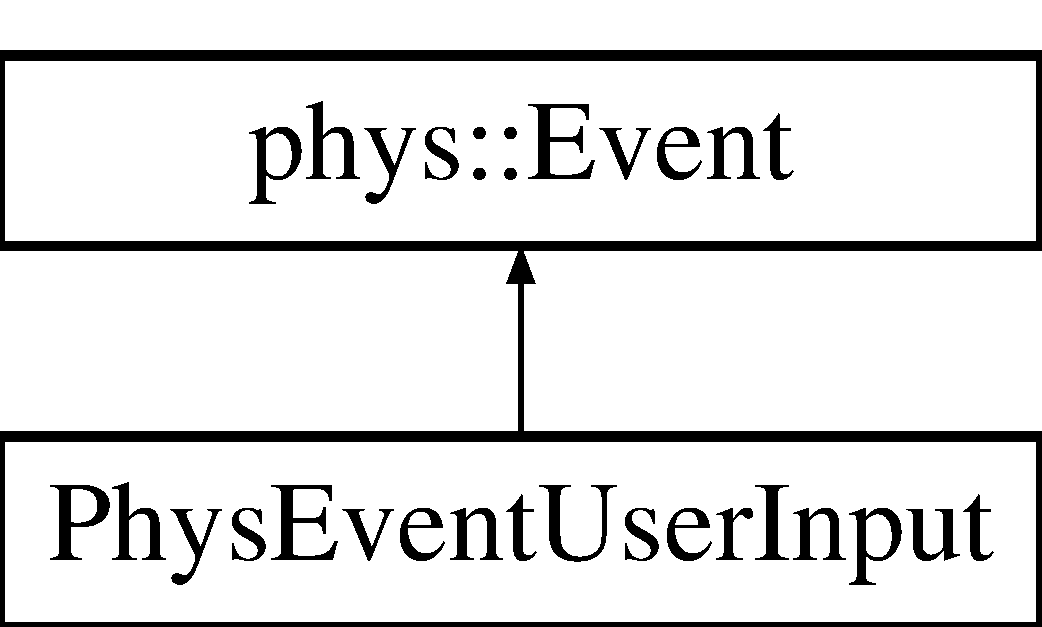
\includegraphics[height=2cm]{dc/d0e/classPhysEventUserInput}
\end{center}
\end{figure}
\subsection*{Public Member Functions}
\begin{DoxyCompactItemize}
\item 
\hyperlink{classPhysEventUserInput_a6f8eaf698e8109d5cb30f2f17044f1ba}{PhysEventUserInput} ()
\begin{DoxyCompactList}\small\item\em Default constructor. \item\end{DoxyCompactList}\item 
\hyperlink{classPhysEventUserInput_ae13b1b02bfa3ef64dc4205478a68810f}{PhysEventUserInput} (const \hyperlink{classMetaCode}{MetaCode} \&Code\_\-)
\begin{DoxyCompactList}\small\item\em Single Data Point constructor. \item\end{DoxyCompactList}\item 
\hyperlink{classPhysEventUserInput_a0a9bd99d8db6f171ef3c87bd417ccc4a}{PhysEventUserInput} (const vector$<$ \hyperlink{classMetaCode}{MetaCode} $>$ \&Codes\_\-)
\begin{DoxyCompactList}\small\item\em Multi Data Point constructor. \item\end{DoxyCompactList}\item 
const \hyperlink{classMetaCode}{MetaCode} \hyperlink{classPhysEventUserInput_aa564530c27f6983bb412e46c2c7ed086}{GetMetaCode} (const unsigned int \&Index)
\begin{DoxyCompactList}\small\item\em Single Data Point constructor. \item\end{DoxyCompactList}\item 
unsigned int \hyperlink{classPhysEventUserInput_a86df812a38566a572134100a422a8799}{GetMetaCodeCount} ()
\begin{DoxyCompactList}\small\item\em Retrieves a count of the stored Metacodes. \item\end{DoxyCompactList}\item 
void \hyperlink{classPhysEventUserInput_a4f5b94c64cd08c15b480e441d25a385d}{AddCode} (const \hyperlink{classMetaCode}{MetaCode} \&Code\_\-)
\begin{DoxyCompactList}\small\item\em Adds a \hyperlink{classMetaCode}{MetaCode}. \item\end{DoxyCompactList}\item 
void \hyperlink{classPhysEventUserInput_ace3b98a502b8e784b58bc5dc599fc0c4}{AddCode} (const int \&MetaValue\_\-, const short unsigned int \&ID\_\-, const \hyperlink{classMetaCode_a7390e6f58e25c0ce377bba4e63081b24}{MetaCode::InputCode} \&Code\_\-)
\begin{DoxyCompactList}\small\item\em Adds a Created From Raw Values. \item\end{DoxyCompactList}\item 
void \hyperlink{classPhysEventUserInput_a385a4f7a6e88be43b6ba1ffc2a1bb5e3}{AddCode} (const RawEvent \&RawEvent\_\-)
\begin{DoxyCompactList}\small\item\em Adds a \hyperlink{classMetaCode}{MetaCode} created from a RawEvent. \item\end{DoxyCompactList}\item 
void \hyperlink{classPhysEventUserInput_aecac02073d3296c71e0ae4534daf8dce}{AddCode} (const vector$<$ \hyperlink{classMetaCode}{MetaCode} $>$ \&Codes)
\begin{DoxyCompactList}\small\item\em Add Several MetaCodes from a vector. \item\end{DoxyCompactList}\item 
void \hyperlink{classPhysEventUserInput_a9e42f42f9a4a42f792e5cf95856669c0}{AddCodesFromRawEvent} (const RawEvent \&RawEvent\_\-)
\begin{DoxyCompactList}\small\item\em Adds all possible MetaCodes that can be created from the given RawEvent. \item\end{DoxyCompactList}\item 
void \hyperlink{classPhysEventUserInput_a1dbd2996770df334fba9f67d9bb4ffa0}{EraseCode} (const \hyperlink{classMetaCode}{MetaCode} \&Code\_\-)
\begin{DoxyCompactList}\small\item\em Removes a specific code from storage. \item\end{DoxyCompactList}\item 
void \hyperlink{classPhysEventUserInput_a8cbbee3c2be3bd12746ad442fce526e4}{EraseCode} (const unsigned int \&Index)
\begin{DoxyCompactList}\small\item\em Removes a specific code from storage. \item\end{DoxyCompactList}\item 
void \hyperlink{classPhysEventUserInput_a8325bb0172db6ea02fd06f4a5d1a7378}{ToggleCode} (const \hyperlink{classMetaCode}{MetaCode} \&Code\_\-)
\begin{DoxyCompactList}\small\item\em Removes a specific code or Adds it if not present. \item\end{DoxyCompactList}\item 
\hyperlink{classPhysEventUserInput}{PhysEventUserInput} \& \hyperlink{classPhysEventUserInput_a257c2e093b5736324e39d5fac0d6de2a}{operator+=} (const \hyperlink{classPhysEventUserInput}{PhysEventUserInput} \&Add)
\begin{DoxyCompactList}\small\item\em This add all of one \hyperlink{classPhysEventUserInput}{PhysEventUserInput} to another. \item\end{DoxyCompactList}\item 
virtual EventType \hyperlink{classPhysEventUserInput_ab89b06b8f7aa148cad453ca9fcae5b89}{getEventType} ()
\begin{DoxyCompactList}\small\item\em Returns the type of this event. \item\end{DoxyCompactList}\end{DoxyCompactItemize}
\subsection*{Protected Attributes}
\begin{DoxyCompactItemize}
\item 
\hypertarget{classPhysEventUserInput_a51607772d8a5b9f401ad0efc964ec129}{
vector$<$ \hyperlink{classMetaCode}{MetaCode} $>$ {\bfseries Code}}
\label{dc/d0e/classPhysEventUserInput_a51607772d8a5b9f401ad0efc964ec129}

\end{DoxyCompactItemize}


\subsection{Detailed Description}
This is a container for MetaCodes that is used in the physEventManager. The \hyperlink{classPhysEventUserInput}{PhysEventUserInput} is the container for information about how a user enters data and commands into a program. By Default one is inserted into event manager the with all the user input from the last run of the main loop. These can be manually inserted into the EventManager to simulate input from other sources. If setup properly this can allow computer controlled characters to use the same interface players, allowing for more realistic response from them. This is not limited to the tricks discussed here. 

Definition at line 93 of file physeventuserinput.h.

\subsection{Constructor \& Destructor Documentation}
\hypertarget{classPhysEventUserInput_a6f8eaf698e8109d5cb30f2f17044f1ba}{
\index{PhysEventUserInput@{PhysEventUserInput}!PhysEventUserInput@{PhysEventUserInput}}
\index{PhysEventUserInput@{PhysEventUserInput}!PhysEventUserInput@{PhysEventUserInput}}
\subsubsection[{PhysEventUserInput}]{\setlength{\rightskip}{0pt plus 5cm}PhysEventUserInput::PhysEventUserInput ()}}
\label{dc/d0e/classPhysEventUserInput_a6f8eaf698e8109d5cb30f2f17044f1ba}


Default constructor. This creates a perfectly functional, but empty \hyperlink{classPhysEventUserInput}{PhysEventUserInput}. 

Definition at line 64 of file physeventuserinput.cpp.\hypertarget{classPhysEventUserInput_ae13b1b02bfa3ef64dc4205478a68810f}{
\index{PhysEventUserInput@{PhysEventUserInput}!PhysEventUserInput@{PhysEventUserInput}}
\index{PhysEventUserInput@{PhysEventUserInput}!PhysEventUserInput@{PhysEventUserInput}}
\subsubsection[{PhysEventUserInput}]{\setlength{\rightskip}{0pt plus 5cm}PhysEventUserInput::PhysEventUserInput (const {\bf MetaCode} \& {\em Code\_\-})}}
\label{dc/d0e/classPhysEventUserInput_ae13b1b02bfa3ef64dc4205478a68810f}


Single Data Point constructor. 
\begin{DoxyParams}{Parameters}
\item[{\em Code\_\-}]This \hyperlink{classMetaCode}{MetaCode} will be added to the \hyperlink{classPhysEventUserInput}{PhysEventUserInput} during creation.\end{DoxyParams}
This creates a functional \hyperlink{classPhysEventUserInput}{PhysEventUserInput} which already contains one metacode. 

Definition at line 69 of file physeventuserinput.cpp.\hypertarget{classPhysEventUserInput_a0a9bd99d8db6f171ef3c87bd417ccc4a}{
\index{PhysEventUserInput@{PhysEventUserInput}!PhysEventUserInput@{PhysEventUserInput}}
\index{PhysEventUserInput@{PhysEventUserInput}!PhysEventUserInput@{PhysEventUserInput}}
\subsubsection[{PhysEventUserInput}]{\setlength{\rightskip}{0pt plus 5cm}PhysEventUserInput::PhysEventUserInput (const vector$<$ {\bf MetaCode} $>$ \& {\em Codes\_\-})}}
\label{dc/d0e/classPhysEventUserInput_a0a9bd99d8db6f171ef3c87bd417ccc4a}


Multi Data Point constructor. 
\begin{DoxyParams}{Parameters}
\item[{\em Code\_\-}]The MetaCodes in this vecotor will be added to the \hyperlink{classPhysEventUserInput}{PhysEventUserInput} during creation.\end{DoxyParams}
This creates a ready to use \hyperlink{classPhysEventUserInput}{PhysEventUserInput} which already contains all the metacodes included. 

Definition at line 74 of file physeventuserinput.cpp.

\subsection{Member Function Documentation}
\hypertarget{classPhysEventUserInput_aecac02073d3296c71e0ae4534daf8dce}{
\index{PhysEventUserInput@{PhysEventUserInput}!AddCode@{AddCode}}
\index{AddCode@{AddCode}!PhysEventUserInput@{PhysEventUserInput}}
\subsubsection[{AddCode}]{\setlength{\rightskip}{0pt plus 5cm}void PhysEventUserInput::AddCode (const vector$<$ {\bf MetaCode} $>$ \& {\em Codes})}}
\label{dc/d0e/classPhysEventUserInput_aecac02073d3296c71e0ae4534daf8dce}


Add Several MetaCodes from a vector. 
\begin{DoxyParams}{Parameters}
\item[{\em Codes\_\-}]A vector of MetaCodes to be added to this event\end{DoxyParams}
This adds several existing metacodes to this event. 

Definition at line 111 of file physeventuserinput.cpp.\hypertarget{classPhysEventUserInput_a385a4f7a6e88be43b6ba1ffc2a1bb5e3}{
\index{PhysEventUserInput@{PhysEventUserInput}!AddCode@{AddCode}}
\index{AddCode@{AddCode}!PhysEventUserInput@{PhysEventUserInput}}
\subsubsection[{AddCode}]{\setlength{\rightskip}{0pt plus 5cm}void PhysEventUserInput::AddCode (const RawEvent \& {\em RawEvent\_\-})}}
\label{dc/d0e/classPhysEventUserInput_a385a4f7a6e88be43b6ba1ffc2a1bb5e3}


Adds a \hyperlink{classMetaCode}{MetaCode} created from a RawEvent. 
\begin{DoxyParams}{Parameters}
\item[{\em RawEvent\_\-}]The RawEvent which will be translated into exactly One \hyperlink{classMetaCode}{MetaCode}\end{DoxyParams}
This will add \hyperlink{classMetaCode}{MetaCode} to this event which will be create from a RawEvent which can produce Exactly one \hyperlink{classMetaCode}{MetaCode}. This is used by engine internals, it is recommended to not use this in game code. \begin{DoxyWarning}{Warning}
Do not use this without reading and fully understanding the warnings on \hyperlink{classMetaCode_a87b260ce7ee3a66c75320c0fc37cdc0a}{MetaCode::MetaCode(const RawEvent \&RawEvent\_\-)} . This function has all the same Restrictions. If game code is using RawEvents at all, the game logic should be scrutinized carefully, it is probably wrong, but if it must it should use \hyperlink{classPhysEventUserInput_a9e42f42f9a4a42f792e5cf95856669c0}{PhysEventUserInput::AddCodesFromRawEvent} instead, as it can make the needed determinations automatically and in a platform agnostic way. 
\end{DoxyWarning}


Definition at line 99 of file physeventuserinput.cpp.\hypertarget{classPhysEventUserInput_ace3b98a502b8e784b58bc5dc599fc0c4}{
\index{PhysEventUserInput@{PhysEventUserInput}!AddCode@{AddCode}}
\index{AddCode@{AddCode}!PhysEventUserInput@{PhysEventUserInput}}
\subsubsection[{AddCode}]{\setlength{\rightskip}{0pt plus 5cm}void PhysEventUserInput::AddCode (const int \& {\em MetaValue\_\-}, \/  const short unsigned int \& {\em ID\_\-}, \/  const {\bf MetaCode::InputCode} \& {\em Code\_\-})}}
\label{dc/d0e/classPhysEventUserInput_ace3b98a502b8e784b58bc5dc599fc0c4}


Adds a Created From Raw Values. 
\begin{DoxyParams}{Parameters}
\item[{\em MetaValue\_\-}]The MetaValue that will be in the \hyperlink{classMetaCode}{MetaCode} \item[{\em ID\_\-}]The ID that will be in the \hyperlink{classMetaCode}{MetaCode} \item[{\em Code\_\-}]The InputCode that will be in the \hyperlink{classMetaCode}{MetaCode}\end{DoxyParams}
This creates metacode a metacode and adds it to this event. 

Definition at line 105 of file physeventuserinput.cpp.\hypertarget{classPhysEventUserInput_a4f5b94c64cd08c15b480e441d25a385d}{
\index{PhysEventUserInput@{PhysEventUserInput}!AddCode@{AddCode}}
\index{AddCode@{AddCode}!PhysEventUserInput@{PhysEventUserInput}}
\subsubsection[{AddCode}]{\setlength{\rightskip}{0pt plus 5cm}void PhysEventUserInput::AddCode (const {\bf MetaCode} \& {\em Code\_\-})}}
\label{dc/d0e/classPhysEventUserInput_a4f5b94c64cd08c15b480e441d25a385d}


Adds a \hyperlink{classMetaCode}{MetaCode}. 
\begin{DoxyParams}{Parameters}
\item[{\em Code\_\-}]The User Input \hyperlink{classMetaCode}{MetaCode} tobe added\end{DoxyParams}
This adds an existing metacode to this event. 

Definition at line 94 of file physeventuserinput.cpp.\hypertarget{classPhysEventUserInput_a9e42f42f9a4a42f792e5cf95856669c0}{
\index{PhysEventUserInput@{PhysEventUserInput}!AddCodesFromRawEvent@{AddCodesFromRawEvent}}
\index{AddCodesFromRawEvent@{AddCodesFromRawEvent}!PhysEventUserInput@{PhysEventUserInput}}
\subsubsection[{AddCodesFromRawEvent}]{\setlength{\rightskip}{0pt plus 5cm}void PhysEventUserInput::AddCodesFromRawEvent (const RawEvent \& {\em RawEvent\_\-})}}
\label{dc/d0e/classPhysEventUserInput_a9e42f42f9a4a42f792e5cf95856669c0}


Adds all possible MetaCodes that can be created from the given RawEvent. 
\begin{DoxyParams}{Parameters}
\item[{\em RawEvent\_\-}]The RawEvent which will be translated into a group of metacodes and added to this\end{DoxyParams}
This will add \hyperlink{classMetaCode}{MetaCode} to this event which will be create from a RawEvent which can produce Exactly one \hyperlink{classMetaCode}{MetaCode}. This is used by engine internals, it is recommended to not use this in game code. \begin{DoxyWarning}{Warning}
If game code is using RawEvents at all, the game logic should be scrutinized carefully, it is probably wrong, but if it must them this is the correct function to use. This will work same on a all platforms. However, the binary format of the Rawevent could chnage meaning you would have to recompile the game code to work with new version of the engine \par
 This Function is currently incomplete, and does not yet process all events such as joysticks events and some mouse events. 
\end{DoxyWarning}


Definition at line 162 of file physeventuserinput.cpp.\hypertarget{classPhysEventUserInput_a8cbbee3c2be3bd12746ad442fce526e4}{
\index{PhysEventUserInput@{PhysEventUserInput}!EraseCode@{EraseCode}}
\index{EraseCode@{EraseCode}!PhysEventUserInput@{PhysEventUserInput}}
\subsubsection[{EraseCode}]{\setlength{\rightskip}{0pt plus 5cm}void PhysEventUserInput::EraseCode (const unsigned int \& {\em Index})}}
\label{dc/d0e/classPhysEventUserInput_a8cbbee3c2be3bd12746ad442fce526e4}


Removes a specific code from storage. 
\begin{DoxyParams}{Parameters}
\item[{\em Index}]This is the location to removed from\end{DoxyParams}
The \hyperlink{classMetaCode}{MetaCode} at and only at the given Index will be deleted. 

Definition at line 133 of file physeventuserinput.cpp.\hypertarget{classPhysEventUserInput_a1dbd2996770df334fba9f67d9bb4ffa0}{
\index{PhysEventUserInput@{PhysEventUserInput}!EraseCode@{EraseCode}}
\index{EraseCode@{EraseCode}!PhysEventUserInput@{PhysEventUserInput}}
\subsubsection[{EraseCode}]{\setlength{\rightskip}{0pt plus 5cm}void PhysEventUserInput::EraseCode (const {\bf MetaCode} \& {\em Code\_\-})}}
\label{dc/d0e/classPhysEventUserInput_a1dbd2996770df334fba9f67d9bb4ffa0}


Removes a specific code from storage. 
\begin{DoxyParams}{Parameters}
\item[{\em Code\_\-}]This will search for all matching copies of this\end{DoxyParams}
All MetaCodes that are equal to Code\_\- will simply be erased. 

Definition at line 120 of file physeventuserinput.cpp.\hypertarget{classPhysEventUserInput_ab89b06b8f7aa148cad453ca9fcae5b89}{
\index{PhysEventUserInput@{PhysEventUserInput}!getEventType@{getEventType}}
\index{getEventType@{getEventType}!PhysEventUserInput@{PhysEventUserInput}}
\subsubsection[{getEventType}]{\setlength{\rightskip}{0pt plus 5cm}PhysEvent::EventType PhysEventUserInput::getEventType ()\hspace{0.3cm}{\ttfamily  \mbox{[}virtual\mbox{]}}}}
\label{dc/d0e/classPhysEventUserInput_ab89b06b8f7aa148cad453ca9fcae5b89}


Returns the type of this event. \begin{DoxyReturn}{Returns}
Returns EventType::UserInput 
\end{DoxyReturn}


Implements \hyperlink{classPhysEvent}{PhysEvent}.

Definition at line 157 of file physeventuserinput.cpp.\hypertarget{classPhysEventUserInput_aa564530c27f6983bb412e46c2c7ed086}{
\index{PhysEventUserInput@{PhysEventUserInput}!GetMetaCode@{GetMetaCode}}
\index{GetMetaCode@{GetMetaCode}!PhysEventUserInput@{PhysEventUserInput}}
\subsubsection[{GetMetaCode}]{\setlength{\rightskip}{0pt plus 5cm}const {\bf MetaCode} PhysEventUserInput::GetMetaCode (const unsigned int \& {\em Index})}}
\label{dc/d0e/classPhysEventUserInput_aa564530c27f6983bb412e46c2c7ed086}


Single Data Point constructor. 
\begin{DoxyParams}{Parameters}
\item[{\em Code\_\-}]which Metacode to return. \end{DoxyParams}
\begin{DoxyReturn}{Returns}
Index The requested \hyperlink{classMetaCode}{MetaCode}
\end{DoxyReturn}
This function simply retrieves the requested \hyperlink{classMetaCode}{MetaCode}. It can throw standard Out of bounds exceptions if attemped to reference a negative item or an item with Index higher than what exists \par
 This is useful for accessing each \hyperlink{classMetaCode}{MetaCode} stored in this physUserInputEvent. 

Definition at line 84 of file physeventuserinput.cpp.\hypertarget{classPhysEventUserInput_a86df812a38566a572134100a422a8799}{
\index{PhysEventUserInput@{PhysEventUserInput}!GetMetaCodeCount@{GetMetaCodeCount}}
\index{GetMetaCodeCount@{GetMetaCodeCount}!PhysEventUserInput@{PhysEventUserInput}}
\subsubsection[{GetMetaCodeCount}]{\setlength{\rightskip}{0pt plus 5cm}unsigned int PhysEventUserInput::GetMetaCodeCount ()}}
\label{dc/d0e/classPhysEventUserInput_a86df812a38566a572134100a422a8799}


Retrieves a count of the stored Metacodes. \begin{DoxyReturn}{Returns}
The amount of codes stored in this physEventUserInput. 
\end{DoxyReturn}


Definition at line 89 of file physeventuserinput.cpp.\hypertarget{classPhysEventUserInput_a257c2e093b5736324e39d5fac0d6de2a}{
\index{PhysEventUserInput@{PhysEventUserInput}!operator+=@{operator+=}}
\index{operator+=@{operator+=}!PhysEventUserInput@{PhysEventUserInput}}
\subsubsection[{operator+=}]{\setlength{\rightskip}{0pt plus 5cm}{\bf PhysEventUserInput} \& PhysEventUserInput::operator+= (const {\bf PhysEventUserInput} \& {\em Add})}}
\label{dc/d0e/classPhysEventUserInput_a257c2e093b5736324e39d5fac0d6de2a}


This add all of one \hyperlink{classPhysEventUserInput}{PhysEventUserInput} to another. 
\begin{DoxyParams}{Parameters}
\item[{\em Add}]is the \hyperlink{classPhysEventUserInput}{PhysEventUserInput} on the right hand side of +=\end{DoxyParams}
This simply copies all the MetaCodes from one \hyperlink{classPhysEventUserInput}{PhysEventUserInput} to the other. \begin{DoxyReturn}{Returns}
The \hyperlink{classPhysEventUserInput}{PhysEventUserInput} on the left ahnd side will now contain a set of both items MetaCodes 
\end{DoxyReturn}


Definition at line 195 of file physeventuserinput.cpp.\hypertarget{classPhysEventUserInput_a8325bb0172db6ea02fd06f4a5d1a7378}{
\index{PhysEventUserInput@{PhysEventUserInput}!ToggleCode@{ToggleCode}}
\index{ToggleCode@{ToggleCode}!PhysEventUserInput@{PhysEventUserInput}}
\subsubsection[{ToggleCode}]{\setlength{\rightskip}{0pt plus 5cm}void PhysEventUserInput::ToggleCode (const {\bf MetaCode} \& {\em Code\_\-})}}
\label{dc/d0e/classPhysEventUserInput_a8325bb0172db6ea02fd06f4a5d1a7378}


Removes a specific code or Adds it if not present. 
\begin{DoxyParams}{Parameters}
\item[{\em Code\_\-}]This will search for all matching copies of this.\end{DoxyParams}
All MetaCodes that are equal to Code\_\- will simply be erased. 

Definition at line 138 of file physeventuserinput.cpp.

The documentation for this class was generated from the following files:\begin{DoxyCompactItemize}
\item 
physeventuserinput.h\item 
physeventuserinput.cpp\end{DoxyCompactItemize}

\hypertarget{classphys_1_1PhysMotionState}{
\section{phys::PhysMotionState Class Reference}
\label{dc/d0d/classphys_1_1PhysMotionState}\index{phys::PhysMotionState@{phys::PhysMotionState}}
}


This class is used by the actor class to sync between the physics world and the graphical world.  




{\ttfamily \#include $<$physactor.h$>$}

\subsection*{Public Member Functions}
\begin{DoxyCompactItemize}
\item 
\hyperlink{classphys_1_1PhysMotionState_ac685ae94d7ee7740aaee8c1a1132b27a}{PhysMotionState} ()
\begin{DoxyCompactList}\small\item\em Blank Constructor. \item\end{DoxyCompactList}\item 
\hyperlink{classphys_1_1PhysMotionState_a505aa5ea3bbaba4710924f030f4ed008}{PhysMotionState} (Ogre::SceneNode $\ast$scenenode)
\begin{DoxyCompactList}\small\item\em Constructor. \item\end{DoxyCompactList}\item 
virtual \hyperlink{classphys_1_1PhysMotionState_a20798e3dce2d71a938c3607a8610eaac}{$\sim$PhysMotionState} ()
\begin{DoxyCompactList}\small\item\em Destructor. \item\end{DoxyCompactList}\item 
void \hyperlink{classphys_1_1PhysMotionState_a034376e768543b377430611dff323412}{SetNode} (Ogre::SceneNode $\ast$scenenode)
\begin{DoxyCompactList}\small\item\em Sets the scenenode. \item\end{DoxyCompactList}\item 
void \hyperlink{classphys_1_1PhysMotionState_a083029e5dbcfafd573d47331ff8660cb}{SetPosition} (\hyperlink{classPhysVector3}{PhysVector3} position)
\begin{DoxyCompactList}\small\item\em Sets the initial position. \item\end{DoxyCompactList}\item 
void \hyperlink{classphys_1_1PhysMotionState_ac799070edfea4d1c442e3ed0857bcb1d}{SetOrientation} (\hyperlink{classphys_1_1Quaternion}{Quaternion} orientation)
\begin{DoxyCompactList}\small\item\em Sets the initial orientation. \item\end{DoxyCompactList}\item 
virtual void \hyperlink{classphys_1_1PhysMotionState_a80e8549fbab99150ba8f34aa3bf087d8}{getWorldTransform} (btTransform \&worldTrans) const 
\begin{DoxyCompactList}\small\item\em Sets the initial position. \item\end{DoxyCompactList}\item 
virtual void \hyperlink{classphys_1_1PhysMotionState_a91e372f8f474bb570e502ee42ec2deeb}{setWorldTransform} (const btTransform \&worldTrans)
\begin{DoxyCompactList}\small\item\em Updates the position and orientation. \item\end{DoxyCompactList}\end{DoxyCompactItemize}
\subsection*{Friends}
\begin{DoxyCompactItemize}
\item 
\hypertarget{classphys_1_1PhysMotionState_ac09063d4b0192680ba3aa0bd4003a274}{
class {\bfseries ActorBase}}
\label{dc/d0d/classphys_1_1PhysMotionState_ac09063d4b0192680ba3aa0bd4003a274}

\end{DoxyCompactItemize}


\subsection{Detailed Description}
This class is used by the actor class to sync between the physics world and the graphical world. This class provides the link for position and orientation between the two worlds in the engine. This is called on every step(frame) of the world to sync the actor if it has moved. 

Definition at line 62 of file physactor.cpp.



\subsection{Constructor \& Destructor Documentation}
\hypertarget{classphys_1_1PhysMotionState_ac685ae94d7ee7740aaee8c1a1132b27a}{
\index{phys::PhysMotionState@{phys::PhysMotionState}!PhysMotionState@{PhysMotionState}}
\index{PhysMotionState@{PhysMotionState}!phys::PhysMotionState@{phys::PhysMotionState}}
\subsubsection[{PhysMotionState}]{\setlength{\rightskip}{0pt plus 5cm}phys::PhysMotionState::PhysMotionState ()}}
\label{dc/d0d/classphys_1_1PhysMotionState_ac685ae94d7ee7740aaee8c1a1132b27a}


Blank Constructor. 

Basic no-\/initialization constructor. 

Definition at line 476 of file physactor.cpp.

\hypertarget{classphys_1_1PhysMotionState_a505aa5ea3bbaba4710924f030f4ed008}{
\index{phys::PhysMotionState@{phys::PhysMotionState}!PhysMotionState@{PhysMotionState}}
\index{PhysMotionState@{PhysMotionState}!phys::PhysMotionState@{phys::PhysMotionState}}
\subsubsection[{PhysMotionState}]{\setlength{\rightskip}{0pt plus 5cm}phys::PhysMotionState::PhysMotionState (Ogre::SceneNode $\ast$ {\em scenenode})}}
\label{dc/d0d/classphys_1_1PhysMotionState_a505aa5ea3bbaba4710924f030f4ed008}


Constructor. 

The class constructor. 
\begin{DoxyParams}{Parameters}
\item[{\em Scenenode}]The scenenode belonging to the actor. \end{DoxyParams}


Definition at line 481 of file physactor.cpp.

\hypertarget{classphys_1_1PhysMotionState_a20798e3dce2d71a938c3607a8610eaac}{
\index{phys::PhysMotionState@{phys::PhysMotionState}!$\sim$PhysMotionState@{$\sim$PhysMotionState}}
\index{$\sim$PhysMotionState@{$\sim$PhysMotionState}!phys::PhysMotionState@{phys::PhysMotionState}}
\subsubsection[{$\sim$PhysMotionState}]{\setlength{\rightskip}{0pt plus 5cm}phys::PhysMotionState::$\sim$PhysMotionState ()\hspace{0.3cm}{\ttfamily  \mbox{[}virtual\mbox{]}}}}
\label{dc/d0d/classphys_1_1PhysMotionState_a20798e3dce2d71a938c3607a8610eaac}


Destructor. 

The class destructor. 

Definition at line 487 of file physactor.cpp.



\subsection{Member Function Documentation}
\hypertarget{classphys_1_1PhysMotionState_a80e8549fbab99150ba8f34aa3bf087d8}{
\index{phys::PhysMotionState@{phys::PhysMotionState}!getWorldTransform@{getWorldTransform}}
\index{getWorldTransform@{getWorldTransform}!phys::PhysMotionState@{phys::PhysMotionState}}
\subsubsection[{getWorldTransform}]{\setlength{\rightskip}{0pt plus 5cm}void phys::PhysMotionState::getWorldTransform (btTransform \& {\em worldTrans}) const\hspace{0.3cm}{\ttfamily  \mbox{[}virtual\mbox{]}}}}
\label{dc/d0d/classphys_1_1PhysMotionState_a80e8549fbab99150ba8f34aa3bf087d8}


Sets the initial position. 

This function is called on by the physics world upon adding the actor to the world. This function uses the previous set vector3 that was set with SetInitPosition(). \par
 Default position is (0,0,0). 
\begin{DoxyParams}{Parameters}
\item[{\em WorldTrans}]The location and orientation data. \end{DoxyParams}


Definition at line 510 of file physactor.cpp.

\hypertarget{classphys_1_1PhysMotionState_a034376e768543b377430611dff323412}{
\index{phys::PhysMotionState@{phys::PhysMotionState}!SetNode@{SetNode}}
\index{SetNode@{SetNode}!phys::PhysMotionState@{phys::PhysMotionState}}
\subsubsection[{SetNode}]{\setlength{\rightskip}{0pt plus 5cm}void phys::PhysMotionState::SetNode (Ogre::SceneNode $\ast$ {\em scenenode})}}
\label{dc/d0d/classphys_1_1PhysMotionState_a034376e768543b377430611dff323412}


Sets the scenenode. 

Sets the scenenode to be sync'd every step. 
\begin{DoxyParams}{Parameters}
\item[{\em Scenenode}]The scenenode belonging to the actor. \end{DoxyParams}


Definition at line 495 of file physactor.cpp.

\hypertarget{classphys_1_1PhysMotionState_ac799070edfea4d1c442e3ed0857bcb1d}{
\index{phys::PhysMotionState@{phys::PhysMotionState}!SetOrientation@{SetOrientation}}
\index{SetOrientation@{SetOrientation}!phys::PhysMotionState@{phys::PhysMotionState}}
\subsubsection[{SetOrientation}]{\setlength{\rightskip}{0pt plus 5cm}void phys::PhysMotionState::SetOrientation ({\bf Quaternion} {\em orientation})}}
\label{dc/d0d/classphys_1_1PhysMotionState_ac799070edfea4d1c442e3ed0857bcb1d}


Sets the initial orientation. 

Sets the orientation the actor will have when it is added to the world. This function is called on by the \hyperlink{classphys_1_1ActorBase}{ActorBase} function SetInitOrientation(). 
\begin{DoxyParams}{Parameters}
\item[{\em Orientation}]The vector3 representing the orientation to be used. \end{DoxyParams}


Definition at line 505 of file physactor.cpp.

\hypertarget{classphys_1_1PhysMotionState_a083029e5dbcfafd573d47331ff8660cb}{
\index{phys::PhysMotionState@{phys::PhysMotionState}!SetPosition@{SetPosition}}
\index{SetPosition@{SetPosition}!phys::PhysMotionState@{phys::PhysMotionState}}
\subsubsection[{SetPosition}]{\setlength{\rightskip}{0pt plus 5cm}void phys::PhysMotionState::SetPosition ({\bf PhysVector3} {\em position})}}
\label{dc/d0d/classphys_1_1PhysMotionState_a083029e5dbcfafd573d47331ff8660cb}


Sets the initial position. 

Sets the position the actor will be placed in when it is added to the world. This function is called on by the \hyperlink{classphys_1_1ActorBase}{ActorBase} function SetInitPosition(). 
\begin{DoxyParams}{Parameters}
\item[{\em Position}]The vector3 representing the location to be used. \end{DoxyParams}


Definition at line 500 of file physactor.cpp.

\hypertarget{classphys_1_1PhysMotionState_a91e372f8f474bb570e502ee42ec2deeb}{
\index{phys::PhysMotionState@{phys::PhysMotionState}!setWorldTransform@{setWorldTransform}}
\index{setWorldTransform@{setWorldTransform}!phys::PhysMotionState@{phys::PhysMotionState}}
\subsubsection[{setWorldTransform}]{\setlength{\rightskip}{0pt plus 5cm}void phys::PhysMotionState::setWorldTransform (const btTransform \& {\em worldTrans})\hspace{0.3cm}{\ttfamily  \mbox{[}virtual\mbox{]}}}}
\label{dc/d0d/classphys_1_1PhysMotionState_a91e372f8f474bb570e502ee42ec2deeb}


Updates the position and orientation. 

This function is called each step(frame) by the physics world to sync the physics and graphical worlds. 
\begin{DoxyParams}{Parameters}
\item[{\em WorldTrans}]The location and orientation data. \end{DoxyParams}


Definition at line 515 of file physactor.cpp.



The documentation for this class was generated from the following file:\begin{DoxyCompactItemize}
\item 
physactor.cpp\end{DoxyCompactItemize}

\hypertarget{classPhysVector3}{
\section{PhysVector3 Class Reference}
\label{da/d11/classPhysVector3}\index{PhysVector3@{PhysVector3}}
}
\subsection*{Public Member Functions}
\begin{DoxyCompactItemize}
\item 
\hypertarget{classPhysVector3_aad8161121a45b20dde0e3cc6959801be}{
{\bfseries PhysVector3} (PhysReal X, PhysReal Y, PhysReal Z)}
\label{da/d11/classPhysVector3_aad8161121a45b20dde0e3cc6959801be}

\item 
\hypertarget{classPhysVector3_adfc5f9e933a94be994ce5ce0c38d1f96}{
btVector3 {\bfseries GetBulletVector3} ()}
\label{da/d11/classPhysVector3_adfc5f9e933a94be994ce5ce0c38d1f96}

\item 
\hypertarget{classPhysVector3_a01facc2b865bb79c589ed1985dd6c49c}{
Ogre::Vector3 {\bfseries GetOgreVector3} ()}
\label{da/d11/classPhysVector3_a01facc2b865bb79c589ed1985dd6c49c}

\end{DoxyCompactItemize}
\subsection*{Public Attributes}
\begin{DoxyCompactItemize}
\item 
\hypertarget{classPhysVector3_ac4586254a6116c616046bd9d5b35ca31}{
PhysReal {\bfseries X}}
\label{da/d11/classPhysVector3_ac4586254a6116c616046bd9d5b35ca31}

\item 
\hypertarget{classPhysVector3_a9bf4609392a492c2b3e278d635ed976a}{
PhysReal {\bfseries Y}}
\label{da/d11/classPhysVector3_a9bf4609392a492c2b3e278d635ed976a}

\item 
\hypertarget{classPhysVector3_a0c0585976cb4c215626e205a2c663226}{
PhysReal {\bfseries Z}}
\label{da/d11/classPhysVector3_a0c0585976cb4c215626e205a2c663226}

\end{DoxyCompactItemize}


\subsection{Detailed Description}


Definition at line 13 of file physvector.h.

The documentation for this class was generated from the following files:\begin{DoxyCompactItemize}
\item 
physvector.h\item 
physvector.cpp\end{DoxyCompactItemize}

\hypertarget{classphys_1_1Quaternion}{
\subsection{phys::Quaternion Class Reference}
\label{classphys_1_1Quaternion}\index{phys::Quaternion@{phys::Quaternion}}
}


This is used to store information about rotation in 3d space.  




{\ttfamily \#include $<$quaternion.h$>$}

\subsubsection*{Public Member Functions}
\begin{DoxyCompactItemize}
\item 
\hyperlink{namespacephys_af7eb897198d265b8e868f45240230d5f}{Real} \hyperlink{classphys_1_1Quaternion_a249938e4221bf91c0853d7ff28b42392}{DotProduct} (const \hyperlink{classphys_1_1Quaternion}{Quaternion} \&Other) const 
\begin{DoxyCompactList}\small\item\em Gets the Dot Product of this quaternion and another quaternion. \item\end{DoxyCompactList}\item 
void \hyperlink{classphys_1_1Quaternion_a10d3582b2731e70279d7bab43173f317}{ExtractBulletQuaternion} (const btQuaternion \&Ours)
\begin{DoxyCompactList}\small\item\em Copies an existing Bullet quaternion. \item\end{DoxyCompactList}\item 
void \hyperlink{classphys_1_1Quaternion_a942fab675a0b124e1dc5e2febab113e6}{ExtractOgreQuaternion} (const Ogre::Quaternion \&Ours)
\begin{DoxyCompactList}\small\item\em Copies an existing Ogre quaternion. \item\end{DoxyCompactList}\item 
btQuaternion \hyperlink{classphys_1_1Quaternion_a053f994770b600ae153a142bb4ba7d33}{GetBulletQuaternion} (bool normalize=false) const 
\begin{DoxyCompactList}\small\item\em Gets a Bullet quaternion. \item\end{DoxyCompactList}\item 
\hyperlink{classphys_1_1Quaternion}{Quaternion} \hyperlink{classphys_1_1Quaternion_a384833001b14c132553af190e6ebc41e}{GetInverse} () const 
\begin{DoxyCompactList}\small\item\em Inverses this \hyperlink{classphys_1_1Quaternion}{Quaternion}. \item\end{DoxyCompactList}\item 
\hyperlink{classphys_1_1Quaternion}{Quaternion} \hyperlink{classphys_1_1Quaternion_a70d6cf4b57f3e74469089747ef755583}{GetNormalizedCopy} ()
\begin{DoxyCompactList}\small\item\em Get a normalized copy of this \hyperlink{classphys_1_1Quaternion}{Quaternion} without changing this one. \item\end{DoxyCompactList}\item 
Ogre::Quaternion \hyperlink{classphys_1_1Quaternion_aa22645e2e2972007bcf61cd2f8e506d0}{GetOgreQuaternion} (bool normalize=false) const 
\begin{DoxyCompactList}\small\item\em Gets a Ogre quaternion. \item\end{DoxyCompactList}\item 
\hyperlink{namespacephys_af7eb897198d265b8e868f45240230d5f}{Real} \hyperlink{classphys_1_1Quaternion_aaa860619e9370244d1b538dd9aaf0efc}{Length} () const 
\begin{DoxyCompactList}\small\item\em Gets the length of the quaternion. \item\end{DoxyCompactList}\item 
\hyperlink{namespacephys_af7eb897198d265b8e868f45240230d5f}{Real} \hyperlink{classphys_1_1Quaternion_ac81b52051cc7dcb73fa01fb963d068a6}{LengthSqrd} () const 
\begin{DoxyCompactList}\small\item\em Gets the squared length(len$^\wedge$2) of the quaternion. \item\end{DoxyCompactList}\item 
\hyperlink{classphys_1_1Quaternion}{Quaternion} \& \hyperlink{classphys_1_1Quaternion_afafa852e782d0fe20d41bc745c8a4734}{Normalize} ()
\begin{DoxyCompactList}\small\item\em Normalizes this \hyperlink{classphys_1_1Quaternion}{Quaternion}. \item\end{DoxyCompactList}\item 
\hyperlink{classphys_1_1Quaternion}{Quaternion} \hyperlink{classphys_1_1Quaternion_a8a67c3e05a56a38407f899020c61631d}{operator$\ast$} (const \hyperlink{namespacephys_af7eb897198d265b8e868f45240230d5f}{Real} \&Scalar) const 
\begin{DoxyCompactList}\small\item\em Scaling by multiplication. \item\end{DoxyCompactList}\item 
\hyperlink{classphys_1_1Quaternion}{Quaternion} \hyperlink{classphys_1_1Quaternion_a2b1017fc916a896440a00bee3fd3ca9b}{operator$\ast$} (const \hyperlink{classphys_1_1Quaternion}{phys::Quaternion} \&Other) const 
\begin{DoxyCompactList}\small\item\em Multiplication operator with \hyperlink{classphys_1_1Quaternion}{phys::Quaternion} and \hyperlink{classphys_1_1Quaternion}{phys::Quaternion}. \item\end{DoxyCompactList}\item 
\hyperlink{classphys_1_1Quaternion}{Quaternion} \hyperlink{classphys_1_1Quaternion_ae37df9d07e51739908e05a4bd518c1e1}{operator$\ast$} (const Ogre::Quaternion \&Other) const 
\begin{DoxyCompactList}\small\item\em Multiplication operator with \hyperlink{classphys_1_1Quaternion}{phys::Quaternion} and Ogre::Quaternion. \item\end{DoxyCompactList}\item 
\hyperlink{classphys_1_1Quaternion}{Quaternion} \hyperlink{classphys_1_1Quaternion_abafe5f21ebfac271310905b29da13373}{operator$\ast$} (const btQuaternion \&Other) const 
\begin{DoxyCompactList}\small\item\em Multiplication operator with \hyperlink{classphys_1_1Quaternion}{phys::Quaternion} and btQuaternion. \item\end{DoxyCompactList}\item 
\hyperlink{classphys_1_1Vector3}{Vector3} \hyperlink{classphys_1_1Quaternion_a4e3107c95f94d2b4ddae8c86be9fe28e}{operator$\ast$} (const \hyperlink{classphys_1_1Vector3}{Vector3} \&Other) const 
\begin{DoxyCompactList}\small\item\em Rotates a vector by the provided vector. \item\end{DoxyCompactList}\item 
\hyperlink{classphys_1_1Quaternion}{Quaternion} \hyperlink{classphys_1_1Quaternion_af3f9a9b5835400dc5b83ba06bf9845b0}{operator+} (const \hyperlink{classphys_1_1Quaternion}{phys::Quaternion} \&Other) const 
\begin{DoxyCompactList}\small\item\em Addition operator with \hyperlink{classphys_1_1Quaternion}{phys::Quaternion} and \hyperlink{classphys_1_1Quaternion}{phys::Quaternion}. \item\end{DoxyCompactList}\item 
\hyperlink{classphys_1_1Quaternion}{Quaternion} \hyperlink{classphys_1_1Quaternion_a71fcb37dae7602349e856b202ca00e89}{operator+} (const Ogre::Quaternion \&Other) const 
\begin{DoxyCompactList}\small\item\em Addition operator with \hyperlink{classphys_1_1Quaternion}{phys::Quaternion} and Ogre::Quaternion. \item\end{DoxyCompactList}\item 
\hyperlink{classphys_1_1Quaternion}{Quaternion} \hyperlink{classphys_1_1Quaternion_a3dc35eeb41c43ce79fdf2fc64fc15532}{operator+} (const btQuaternion \&Other) const 
\begin{DoxyCompactList}\small\item\em Addition operator with \hyperlink{classphys_1_1Quaternion}{phys::Quaternion} and btQuaternion. \item\end{DoxyCompactList}\item 
\hyperlink{classphys_1_1Quaternion}{Quaternion} \& \hyperlink{classphys_1_1Quaternion_ab167530770fb0463c5473b5f533db9a8}{operator+=} (const btQuaternion \&Other)
\begin{DoxyCompactList}\small\item\em Incrementing operator with \hyperlink{classphys_1_1Quaternion}{phys::Quaternion} and btQuaternion. \item\end{DoxyCompactList}\item 
\hyperlink{classphys_1_1Quaternion}{Quaternion} \& \hyperlink{classphys_1_1Quaternion_a5d9d2ee516e4e142417b21eecf2e94ce}{operator+=} (const \hyperlink{classphys_1_1Quaternion}{phys::Quaternion} \&Other)
\begin{DoxyCompactList}\small\item\em Incrementing operator with \hyperlink{classphys_1_1Quaternion}{phys::Quaternion} and \hyperlink{classphys_1_1Quaternion}{phys::Quaternion}. \item\end{DoxyCompactList}\item 
\hyperlink{classphys_1_1Quaternion}{Quaternion} \& \hyperlink{classphys_1_1Quaternion_ada6772fd05ec9c8d50b8a25ece3d1c5b}{operator+=} (const Ogre::Quaternion \&Other)
\begin{DoxyCompactList}\small\item\em Incrementing operator with \hyperlink{classphys_1_1Quaternion}{phys::Quaternion} and Ogre::Quaternion. \item\end{DoxyCompactList}\item 
\hyperlink{classphys_1_1Quaternion}{Quaternion} \hyperlink{classphys_1_1Quaternion_abab2d787eefc90bbc6710091a5a79234}{operator-\/} (const \hyperlink{classphys_1_1Quaternion}{phys::Quaternion} \&Other) const 
\begin{DoxyCompactList}\small\item\em Subtraction operator with \hyperlink{classphys_1_1Quaternion}{phys::Quaternion} and \hyperlink{classphys_1_1Quaternion}{phys::Quaternion}. \item\end{DoxyCompactList}\item 
\hyperlink{classphys_1_1Quaternion}{Quaternion} \hyperlink{classphys_1_1Quaternion_a01c5412ce8f1ebb212c9afd7e19feb1e}{operator-\/} (const Ogre::Quaternion \&Other) const 
\begin{DoxyCompactList}\small\item\em Subtraction operator with \hyperlink{classphys_1_1Quaternion}{phys::Quaternion} and Ogre::Quaternion. \item\end{DoxyCompactList}\item 
\hyperlink{classphys_1_1Quaternion}{Quaternion} \hyperlink{classphys_1_1Quaternion_aca49f84681f836545c30c0b42480dccc}{operator-\/} (const btQuaternion \&Other) const 
\begin{DoxyCompactList}\small\item\em Subtraction operator with \hyperlink{classphys_1_1Quaternion}{phys::Quaternion} and btQuaternion. \item\end{DoxyCompactList}\item 
\hyperlink{classphys_1_1Quaternion}{Quaternion} \& \hyperlink{classphys_1_1Quaternion_a66086148dd9154e3e3e0b46bacafe0f7}{operator-\/=} (const \hyperlink{classphys_1_1Quaternion}{phys::Quaternion} \&Other)
\begin{DoxyCompactList}\small\item\em Decrementing operator with \hyperlink{classphys_1_1Quaternion}{phys::Quaternion} and \hyperlink{classphys_1_1Quaternion}{phys::Quaternion}. \item\end{DoxyCompactList}\item 
\hyperlink{classphys_1_1Quaternion}{Quaternion} \& \hyperlink{classphys_1_1Quaternion_af62037687eea0005c9fc4a09355656ed}{operator-\/=} (const Ogre::Quaternion \&Other)
\begin{DoxyCompactList}\small\item\em Decrementing operator with \hyperlink{classphys_1_1Quaternion}{phys::Quaternion} and Ogre::Quaternion. \item\end{DoxyCompactList}\item 
\hyperlink{classphys_1_1Quaternion}{Quaternion} \& \hyperlink{classphys_1_1Quaternion_abd1e9d740b3af194c60466105d07f6ff}{operator-\/=} (const btQuaternion \&Other)
\begin{DoxyCompactList}\small\item\em Decrementing operator with \hyperlink{classphys_1_1Quaternion}{phys::Quaternion} and btQuaternion. \item\end{DoxyCompactList}\item 
\hyperlink{classphys_1_1Quaternion}{Quaternion} \hyperlink{classphys_1_1Quaternion_a9b9492e5a14178aedc784e93b0153364}{operator/} (const \hyperlink{namespacephys_af7eb897198d265b8e868f45240230d5f}{Real} \&Scalar) const 
\begin{DoxyCompactList}\small\item\em Scaling by division. \item\end{DoxyCompactList}\item 
\hyperlink{classphys_1_1Quaternion}{Quaternion} \& \hyperlink{classphys_1_1Quaternion_a6b9fe92548e3fd114d7419ddd5d5a660}{operator=} (const Ogre::Quaternion \&Other)
\begin{DoxyCompactList}\small\item\em Assignment Operator from Ogre::Quaternion. \item\end{DoxyCompactList}\item 
\hyperlink{classphys_1_1Quaternion}{Quaternion} \& \hyperlink{classphys_1_1Quaternion_a05e7364791bf7f38ad63dc59184cd5ca}{operator=} (const btQuaternion \&Other)
\begin{DoxyCompactList}\small\item\em Assignment Operator from btQuaternion. \item\end{DoxyCompactList}\item 
\hyperlink{classphys_1_1Quaternion}{Quaternion} \& \hyperlink{classphys_1_1Quaternion_a6213bddf8f928a8510260b9deb712fd7}{operator=} (const \hyperlink{classphys_1_1Quaternion}{phys::Quaternion} \&Other)
\begin{DoxyCompactList}\small\item\em Assignment Operator from \hyperlink{classphys_1_1Quaternion}{phys::Quaternion}. \item\end{DoxyCompactList}\item 
bool \hyperlink{classphys_1_1Quaternion_a652ec257cb1ab788db646b85f3f89af3}{operator==} (const btQuaternion \&Other) const 
\begin{DoxyCompactList}\small\item\em Equality Comparison Operator from btQuaternion. \item\end{DoxyCompactList}\item 
bool \hyperlink{classphys_1_1Quaternion_a75ab11099a0479885ae5f42945621ef9}{operator==} (const Ogre::Quaternion \&Other) const 
\begin{DoxyCompactList}\small\item\em Equality Comparison Operator from Ogre::Quaternion. \item\end{DoxyCompactList}\item 
bool \hyperlink{classphys_1_1Quaternion_aa02dc20b4246e16017b70788449d7012}{operator==} (const \hyperlink{classphys_1_1Quaternion}{phys::Quaternion} \&Other) const 
\begin{DoxyCompactList}\small\item\em Equality Comparison Operator from \hyperlink{classphys_1_1Quaternion}{phys::Quaternion}. \item\end{DoxyCompactList}\item 
virtual void \hyperlink{classphys_1_1Quaternion_a71e3d4afb129ff822edbc700bae16b4b}{ProtoDeSerialize} (const \hyperlink{classphys_1_1xml_1_1Node}{xml::Node} \&OneNode)
\begin{DoxyCompactList}\small\item\em Take the data stored in an XML and overwrite this instance of this object with it. \item\end{DoxyCompactList}\item 
virtual void \hyperlink{classphys_1_1Quaternion_ab71a780a5103681126d04fec42cdcb2e}{ProtoSerialize} (\hyperlink{classphys_1_1xml_1_1Node}{xml::Node} \&CurrentRoot) const 
\begin{DoxyCompactList}\small\item\em Convert this class to an \hyperlink{classphys_1_1xml_1_1Node}{xml::Node} ready for serialization. \item\end{DoxyCompactList}\item 
\hyperlink{classphys_1_1Quaternion_aca4ee6fd6d3967f06cc4a32361fa5a62}{Quaternion} ()
\begin{DoxyCompactList}\small\item\em Blank Constructor. \item\end{DoxyCompactList}\item 
\hyperlink{classphys_1_1Quaternion_ab9f13d19fe7d602d7c5feaed0aaf4620}{Quaternion} (const btQuaternion \&Theirs)
\begin{DoxyCompactList}\small\item\em Bullet \hyperlink{classphys_1_1Quaternion}{Quaternion} constructor. \item\end{DoxyCompactList}\item 
\hyperlink{classphys_1_1Quaternion_a4902c05489ebae03a55433d947c53d03}{Quaternion} (const Ogre::Quaternion \&Theirs)
\begin{DoxyCompactList}\small\item\em Ogre \hyperlink{classphys_1_1Quaternion}{Quaternion} constructor. \item\end{DoxyCompactList}\item 
\hyperlink{classphys_1_1Quaternion_a46d08f43b0b638a256344b3919ba9e0d}{Quaternion} (const \hyperlink{classphys_1_1Quaternion}{phys::Quaternion} \&Other)
\begin{DoxyCompactList}\small\item\em Copy Constructor. \item\end{DoxyCompactList}\item 
\hyperlink{classphys_1_1Quaternion_ac8037875c08ce10c0195f3e6fd08b172}{Quaternion} (const \hyperlink{namespacephys_af7eb897198d265b8e868f45240230d5f}{Real} \&x, const \hyperlink{namespacephys_af7eb897198d265b8e868f45240230d5f}{Real} \&y, const \hyperlink{namespacephys_af7eb897198d265b8e868f45240230d5f}{Real} \&z, const \hyperlink{namespacephys_af7eb897198d265b8e868f45240230d5f}{Real} \&w)
\begin{DoxyCompactList}\small\item\em Constructor. \item\end{DoxyCompactList}\item 
\hyperlink{classphys_1_1Quaternion_a9246247b7b28f19839148415a7ddeb96}{Quaternion} (const \hyperlink{namespacephys_af7eb897198d265b8e868f45240230d5f}{Real} \&Angle, const \hyperlink{classphys_1_1Vector3}{Vector3} \&Axis)
\begin{DoxyCompactList}\small\item\em Axis and Rotation Constructor. \item\end{DoxyCompactList}\item 
\hyperlink{namespacephys_aa03900411993de7fbfec4789bc1d392e}{String} \hyperlink{classphys_1_1Quaternion_abdfe885d36a7f3c2849a846214fb2872}{SerializableName} () const 
\begin{DoxyCompactList}\small\item\em Get the name of the the XML tag this class will leave behind as its instances are serialized. \item\end{DoxyCompactList}\end{DoxyCompactItemize}
\subsubsection*{Public Attributes}
\begin{DoxyCompactItemize}
\item 
\hypertarget{classphys_1_1Quaternion_af509194048d0cd8fb03d45f150afaa0c}{
\hyperlink{namespacephys_af7eb897198d265b8e868f45240230d5f}{Real} \hyperlink{classphys_1_1Quaternion_af509194048d0cd8fb03d45f150afaa0c}{W}}
\label{classphys_1_1Quaternion_af509194048d0cd8fb03d45f150afaa0c}

\begin{DoxyCompactList}\small\item\em Rotation on the W Axis. \item\end{DoxyCompactList}\item 
\hypertarget{classphys_1_1Quaternion_a29c08e725c7bbb389547cbe03f40f5bd}{
\hyperlink{namespacephys_af7eb897198d265b8e868f45240230d5f}{Real} \hyperlink{classphys_1_1Quaternion_a29c08e725c7bbb389547cbe03f40f5bd}{X}}
\label{classphys_1_1Quaternion_a29c08e725c7bbb389547cbe03f40f5bd}

\begin{DoxyCompactList}\small\item\em Rotation on the X Axis. \item\end{DoxyCompactList}\item 
\hypertarget{classphys_1_1Quaternion_a756165050c3c241fd8b8de6ed21bb268}{
\hyperlink{namespacephys_af7eb897198d265b8e868f45240230d5f}{Real} \hyperlink{classphys_1_1Quaternion_a756165050c3c241fd8b8de6ed21bb268}{Y}}
\label{classphys_1_1Quaternion_a756165050c3c241fd8b8de6ed21bb268}

\begin{DoxyCompactList}\small\item\em Rotation on the Y Axis. \item\end{DoxyCompactList}\item 
\hypertarget{classphys_1_1Quaternion_a708ae111e0cf387b94f33dc7d5b3c59a}{
\hyperlink{namespacephys_af7eb897198d265b8e868f45240230d5f}{Real} \hyperlink{classphys_1_1Quaternion_a708ae111e0cf387b94f33dc7d5b3c59a}{Z}}
\label{classphys_1_1Quaternion_a708ae111e0cf387b94f33dc7d5b3c59a}

\begin{DoxyCompactList}\small\item\em Rotation on the Z Axis. \item\end{DoxyCompactList}\end{DoxyCompactItemize}


\subsubsection{Detailed Description}
This is used to store information about rotation in 3d space. This is used to store information about rotation in 3d space. The X, Y and Z are used to identify a ray from the origin (0,0,0), about which W represents an amount of rotation. \begin{DoxyWarning}{Warning}
The Documentation for this class needs to be revised. It describes 2 mutually exclusive means of storing 
\end{DoxyWarning}


Definition at line 65 of file quaternion.h.



\subsubsection{Constructor \& Destructor Documentation}
\hypertarget{classphys_1_1Quaternion_aca4ee6fd6d3967f06cc4a32361fa5a62}{
\index{phys::Quaternion@{phys::Quaternion}!Quaternion@{Quaternion}}
\index{Quaternion@{Quaternion}!phys::Quaternion@{phys::Quaternion}}
\paragraph[{Quaternion}]{\setlength{\rightskip}{0pt plus 5cm}phys::Quaternion::Quaternion (
\begin{DoxyParamCaption}
{}
\end{DoxyParamCaption}
)}\hfill}
\label{classphys_1_1Quaternion_aca4ee6fd6d3967f06cc4a32361fa5a62}


Blank Constructor. 

Basic no-\/initialization constructor. 

Definition at line 58 of file quaternion.cpp.

\hypertarget{classphys_1_1Quaternion_ac8037875c08ce10c0195f3e6fd08b172}{
\index{phys::Quaternion@{phys::Quaternion}!Quaternion@{Quaternion}}
\index{Quaternion@{Quaternion}!phys::Quaternion@{phys::Quaternion}}
\paragraph[{Quaternion}]{\setlength{\rightskip}{0pt plus 5cm}phys::Quaternion::Quaternion (
\begin{DoxyParamCaption}
\item[{const {\bf Real} \&}]{x, }
\item[{const {\bf Real} \&}]{y, }
\item[{const {\bf Real} \&}]{z, }
\item[{const {\bf Real} \&}]{w}
\end{DoxyParamCaption}
)}\hfill}
\label{classphys_1_1Quaternion_ac8037875c08ce10c0195f3e6fd08b172}


Constructor. 

Constructor that sets all four axis' of rotation. 
\begin{DoxyParams}{Parameters}
{\em x} & Rotation on the X Axis. \\
\hline
{\em y} & Rotation on the Y Axis. \\
\hline
{\em z} & Rotation on the Z Axis. \\
\hline
{\em w} & Rotation on the W Axis. \\
\hline
\end{DoxyParams}


Definition at line 66 of file quaternion.cpp.

\hypertarget{classphys_1_1Quaternion_a9246247b7b28f19839148415a7ddeb96}{
\index{phys::Quaternion@{phys::Quaternion}!Quaternion@{Quaternion}}
\index{Quaternion@{Quaternion}!phys::Quaternion@{phys::Quaternion}}
\paragraph[{Quaternion}]{\setlength{\rightskip}{0pt plus 5cm}phys::Quaternion::Quaternion (
\begin{DoxyParamCaption}
\item[{const {\bf Real} \&}]{Angle, }
\item[{const {\bf Vector3} \&}]{Axis}
\end{DoxyParamCaption}
)}\hfill}
\label{classphys_1_1Quaternion_a9246247b7b28f19839148415a7ddeb96}


Axis and Rotation Constructor. 

This assembles a quaternion based on an axis and a rotation in radians. 
\begin{DoxyParams}{Parameters}
{\em Angle} & Real representing the angle to be applied along the axis in radians. \\
\hline
{\em Axis} & \hyperlink{classphys_1_1Vector3}{Vector3} representing the axis to apply the rotation. \\
\hline
\end{DoxyParams}


\begin{Desc}
\item[\hyperlink{todo__todo000019}{Todo}]Need to find a clean way to wrap sin and cos functions. Also may want to make a radian class/datatype. \end{Desc}




Definition at line 74 of file quaternion.cpp.

\hypertarget{classphys_1_1Quaternion_ab9f13d19fe7d602d7c5feaed0aaf4620}{
\index{phys::Quaternion@{phys::Quaternion}!Quaternion@{Quaternion}}
\index{Quaternion@{Quaternion}!phys::Quaternion@{phys::Quaternion}}
\paragraph[{Quaternion}]{\setlength{\rightskip}{0pt plus 5cm}phys::Quaternion::Quaternion (
\begin{DoxyParamCaption}
\item[{const btQuaternion \&}]{Theirs}
\end{DoxyParamCaption}
)\hspace{0.3cm}{\ttfamily  \mbox{[}explicit\mbox{]}}}\hfill}
\label{classphys_1_1Quaternion_ab9f13d19fe7d602d7c5feaed0aaf4620}


Bullet \hyperlink{classphys_1_1Quaternion}{Quaternion} constructor. 

Constructor that sets all values to match the Bullet quaternion. 
\begin{DoxyParams}{Parameters}
{\em Theirs} & The quaternion to be copied to make this quaternion. \\
\hline
\end{DoxyParams}


Definition at line 85 of file quaternion.cpp.

\hypertarget{classphys_1_1Quaternion_a4902c05489ebae03a55433d947c53d03}{
\index{phys::Quaternion@{phys::Quaternion}!Quaternion@{Quaternion}}
\index{Quaternion@{Quaternion}!phys::Quaternion@{phys::Quaternion}}
\paragraph[{Quaternion}]{\setlength{\rightskip}{0pt plus 5cm}phys::Quaternion::Quaternion (
\begin{DoxyParamCaption}
\item[{const Ogre::Quaternion \&}]{Theirs}
\end{DoxyParamCaption}
)\hspace{0.3cm}{\ttfamily  \mbox{[}explicit\mbox{]}}}\hfill}
\label{classphys_1_1Quaternion_a4902c05489ebae03a55433d947c53d03}


Ogre \hyperlink{classphys_1_1Quaternion}{Quaternion} constructor. 

Constructor that sets all values to match the Ogre quaternion. 
\begin{DoxyParams}{Parameters}
{\em Theirs} & The quaternion to be copied to make this quaternion. \\
\hline
\end{DoxyParams}


Definition at line 88 of file quaternion.cpp.

\hypertarget{classphys_1_1Quaternion_a46d08f43b0b638a256344b3919ba9e0d}{
\index{phys::Quaternion@{phys::Quaternion}!Quaternion@{Quaternion}}
\index{Quaternion@{Quaternion}!phys::Quaternion@{phys::Quaternion}}
\paragraph[{Quaternion}]{\setlength{\rightskip}{0pt plus 5cm}phys::Quaternion::Quaternion (
\begin{DoxyParamCaption}
\item[{const {\bf phys::Quaternion} \&}]{Other}
\end{DoxyParamCaption}
)}\hfill}
\label{classphys_1_1Quaternion_a46d08f43b0b638a256344b3919ba9e0d}


Copy Constructor. 


\begin{DoxyParams}{Parameters}
{\em Other} & The \hyperlink{classphys_1_1Quaternion}{Quaternion} to copy \\
\hline
\end{DoxyParams}


Definition at line 91 of file quaternion.cpp.



\subsubsection{Member Function Documentation}
\hypertarget{classphys_1_1Quaternion_a249938e4221bf91c0853d7ff28b42392}{
\index{phys::Quaternion@{phys::Quaternion}!DotProduct@{DotProduct}}
\index{DotProduct@{DotProduct}!phys::Quaternion@{phys::Quaternion}}
\paragraph[{DotProduct}]{\setlength{\rightskip}{0pt plus 5cm}{\bf Real} phys::Quaternion::DotProduct (
\begin{DoxyParamCaption}
\item[{const {\bf Quaternion} \&}]{Other}
\end{DoxyParamCaption}
) const}\hfill}
\label{classphys_1_1Quaternion_a249938e4221bf91c0853d7ff28b42392}


Gets the Dot Product of this quaternion and another quaternion. 


\begin{DoxyParams}{Parameters}
{\em Other} & The other quaternion to calculate the dot product from. \\
\hline
\end{DoxyParams}
\begin{DoxyReturn}{Returns}
Returns a Real that is the Dot Product of the two quaternions. 
\end{DoxyReturn}


Definition at line 99 of file quaternion.cpp.

\hypertarget{classphys_1_1Quaternion_a10d3582b2731e70279d7bab43173f317}{
\index{phys::Quaternion@{phys::Quaternion}!ExtractBulletQuaternion@{ExtractBulletQuaternion}}
\index{ExtractBulletQuaternion@{ExtractBulletQuaternion}!phys::Quaternion@{phys::Quaternion}}
\paragraph[{ExtractBulletQuaternion}]{\setlength{\rightskip}{0pt plus 5cm}void phys::Quaternion::ExtractBulletQuaternion (
\begin{DoxyParamCaption}
\item[{const btQuaternion \&}]{Ours}
\end{DoxyParamCaption}
)}\hfill}
\label{classphys_1_1Quaternion_a10d3582b2731e70279d7bab43173f317}


Copies an existing Bullet quaternion. 

This function will copy the values stored in an existing Bullet quaternion and set the values of this class to be the same. 
\begin{DoxyParams}{Parameters}
{\em Ours} & The quaternion to be extracted. \\
\hline
\end{DoxyParams}


Definition at line 151 of file quaternion.cpp.

\hypertarget{classphys_1_1Quaternion_a942fab675a0b124e1dc5e2febab113e6}{
\index{phys::Quaternion@{phys::Quaternion}!ExtractOgreQuaternion@{ExtractOgreQuaternion}}
\index{ExtractOgreQuaternion@{ExtractOgreQuaternion}!phys::Quaternion@{phys::Quaternion}}
\paragraph[{ExtractOgreQuaternion}]{\setlength{\rightskip}{0pt plus 5cm}void phys::Quaternion::ExtractOgreQuaternion (
\begin{DoxyParamCaption}
\item[{const Ogre::Quaternion \&}]{Ours}
\end{DoxyParamCaption}
)}\hfill}
\label{classphys_1_1Quaternion_a942fab675a0b124e1dc5e2febab113e6}


Copies an existing Ogre quaternion. 

This function will copy the values stored in an existing Ogre quaternion and set the values of this class to be the same. 
\begin{DoxyParams}{Parameters}
{\em Ours} & The quaternion to be extracted. \\
\hline
\end{DoxyParams}


Definition at line 171 of file quaternion.cpp.

\hypertarget{classphys_1_1Quaternion_a053f994770b600ae153a142bb4ba7d33}{
\index{phys::Quaternion@{phys::Quaternion}!GetBulletQuaternion@{GetBulletQuaternion}}
\index{GetBulletQuaternion@{GetBulletQuaternion}!phys::Quaternion@{phys::Quaternion}}
\paragraph[{GetBulletQuaternion}]{\setlength{\rightskip}{0pt plus 5cm}btQuaternion phys::Quaternion::GetBulletQuaternion (
\begin{DoxyParamCaption}
\item[{bool}]{normalize = {\ttfamily false}}
\end{DoxyParamCaption}
) const}\hfill}
\label{classphys_1_1Quaternion_a053f994770b600ae153a142bb4ba7d33}


Gets a Bullet quaternion. 

Creates a Bullet quaternion with values equal to this class and returns it. 
\begin{DoxyParams}{Parameters}
{\em normalize} & Whether or not you want this function to normalize the quaternion for you. \\
\hline
\end{DoxyParams}
\begin{DoxyReturn}{Returns}
A btQuaternion that has the same contents as this \hyperlink{classphys_1_1Quaternion}{phys::Quaternion}. 
\end{DoxyReturn}


Definition at line 139 of file quaternion.cpp.

\hypertarget{classphys_1_1Quaternion_a384833001b14c132553af190e6ebc41e}{
\index{phys::Quaternion@{phys::Quaternion}!GetInverse@{GetInverse}}
\index{GetInverse@{GetInverse}!phys::Quaternion@{phys::Quaternion}}
\paragraph[{GetInverse}]{\setlength{\rightskip}{0pt plus 5cm}{\bf Quaternion} phys::Quaternion::GetInverse (
\begin{DoxyParamCaption}
{}
\end{DoxyParamCaption}
) const}\hfill}
\label{classphys_1_1Quaternion_a384833001b14c132553af190e6ebc41e}


Inverses this \hyperlink{classphys_1_1Quaternion}{Quaternion}. 

\begin{DoxyReturn}{Returns}
Returns a quaternion that is a copy of this one after it has been inversed. 
\end{DoxyReturn}


Definition at line 124 of file quaternion.cpp.

\hypertarget{classphys_1_1Quaternion_a70d6cf4b57f3e74469089747ef755583}{
\index{phys::Quaternion@{phys::Quaternion}!GetNormalizedCopy@{GetNormalizedCopy}}
\index{GetNormalizedCopy@{GetNormalizedCopy}!phys::Quaternion@{phys::Quaternion}}
\paragraph[{GetNormalizedCopy}]{\setlength{\rightskip}{0pt plus 5cm}{\bf Quaternion} phys::Quaternion::GetNormalizedCopy (
\begin{DoxyParamCaption}
{}
\end{DoxyParamCaption}
)}\hfill}
\label{classphys_1_1Quaternion_a70d6cf4b57f3e74469089747ef755583}


Get a normalized copy of this \hyperlink{classphys_1_1Quaternion}{Quaternion} without changing this one. 

\begin{DoxyReturn}{Returns}
A Copy of this \hyperlink{classphys_1_1Quaternion}{Quaternion} after the copy has been normalized. 
\end{DoxyReturn}


Definition at line 120 of file quaternion.cpp.

\hypertarget{classphys_1_1Quaternion_aa22645e2e2972007bcf61cd2f8e506d0}{
\index{phys::Quaternion@{phys::Quaternion}!GetOgreQuaternion@{GetOgreQuaternion}}
\index{GetOgreQuaternion@{GetOgreQuaternion}!phys::Quaternion@{phys::Quaternion}}
\paragraph[{GetOgreQuaternion}]{\setlength{\rightskip}{0pt plus 5cm}Ogre::Quaternion phys::Quaternion::GetOgreQuaternion (
\begin{DoxyParamCaption}
\item[{bool}]{normalize = {\ttfamily false}}
\end{DoxyParamCaption}
) const}\hfill}
\label{classphys_1_1Quaternion_aa22645e2e2972007bcf61cd2f8e506d0}


Gets a Ogre quaternion. 

Creates a Ogre quaternion with values equal to this class and returns it. 
\begin{DoxyParams}{Parameters}
{\em normalize} & Whether or not you want this function to normalize the quaternion for you. \\
\hline
\end{DoxyParams}


Definition at line 159 of file quaternion.cpp.

\hypertarget{classphys_1_1Quaternion_aaa860619e9370244d1b538dd9aaf0efc}{
\index{phys::Quaternion@{phys::Quaternion}!Length@{Length}}
\index{Length@{Length}!phys::Quaternion@{phys::Quaternion}}
\paragraph[{Length}]{\setlength{\rightskip}{0pt plus 5cm}{\bf Real} phys::Quaternion::Length (
\begin{DoxyParamCaption}
{}
\end{DoxyParamCaption}
) const}\hfill}
\label{classphys_1_1Quaternion_aaa860619e9370244d1b538dd9aaf0efc}


Gets the length of the quaternion. 

\begin{DoxyReturn}{Returns}
Returns a Real representing the length of the quaternion. 
\end{DoxyReturn}


Definition at line 104 of file quaternion.cpp.

\hypertarget{classphys_1_1Quaternion_ac81b52051cc7dcb73fa01fb963d068a6}{
\index{phys::Quaternion@{phys::Quaternion}!LengthSqrd@{LengthSqrd}}
\index{LengthSqrd@{LengthSqrd}!phys::Quaternion@{phys::Quaternion}}
\paragraph[{LengthSqrd}]{\setlength{\rightskip}{0pt plus 5cm}{\bf Real} phys::Quaternion::LengthSqrd (
\begin{DoxyParamCaption}
{}
\end{DoxyParamCaption}
) const}\hfill}
\label{classphys_1_1Quaternion_ac81b52051cc7dcb73fa01fb963d068a6}


Gets the squared length(len$^\wedge$2) of the quaternion. 

\begin{DoxyReturn}{Returns}
Returns a Real representing the squared length(len$^\wedge$2) of the quaternion. 
\end{DoxyReturn}


Definition at line 109 of file quaternion.cpp.

\hypertarget{classphys_1_1Quaternion_afafa852e782d0fe20d41bc745c8a4734}{
\index{phys::Quaternion@{phys::Quaternion}!Normalize@{Normalize}}
\index{Normalize@{Normalize}!phys::Quaternion@{phys::Quaternion}}
\paragraph[{Normalize}]{\setlength{\rightskip}{0pt plus 5cm}{\bf Quaternion} \& phys::Quaternion::Normalize (
\begin{DoxyParamCaption}
{}
\end{DoxyParamCaption}
)}\hfill}
\label{classphys_1_1Quaternion_afafa852e782d0fe20d41bc745c8a4734}


Normalizes this \hyperlink{classphys_1_1Quaternion}{Quaternion}. 

\begin{DoxyReturn}{Returns}
Returns a normalized reference of this quaternion. 
\end{DoxyReturn}


Definition at line 114 of file quaternion.cpp.

\hypertarget{classphys_1_1Quaternion_a2b1017fc916a896440a00bee3fd3ca9b}{
\index{phys::Quaternion@{phys::Quaternion}!operator$\ast$@{operator$\ast$}}
\index{operator$\ast$@{operator$\ast$}!phys::Quaternion@{phys::Quaternion}}
\paragraph[{operator$\ast$}]{\setlength{\rightskip}{0pt plus 5cm}{\bf Quaternion} phys::Quaternion::operator$\ast$ (
\begin{DoxyParamCaption}
\item[{const {\bf phys::Quaternion} \&}]{Other}
\end{DoxyParamCaption}
) const}\hfill}
\label{classphys_1_1Quaternion_a2b1017fc916a896440a00bee3fd3ca9b}


Multiplication operator with \hyperlink{classphys_1_1Quaternion}{phys::Quaternion} and \hyperlink{classphys_1_1Quaternion}{phys::Quaternion}. 


\begin{DoxyParams}{Parameters}
{\em Other} & The other \hyperlink{classphys_1_1Quaternion}{Quaternion} to multiply from this one. \\
\hline
\end{DoxyParams}
\begin{DoxyReturn}{Returns}
A \hyperlink{classphys_1_1Quaternion}{phys::Quaternion} with the result. 
\end{DoxyReturn}


Definition at line 215 of file quaternion.cpp.

\hypertarget{classphys_1_1Quaternion_ae37df9d07e51739908e05a4bd518c1e1}{
\index{phys::Quaternion@{phys::Quaternion}!operator$\ast$@{operator$\ast$}}
\index{operator$\ast$@{operator$\ast$}!phys::Quaternion@{phys::Quaternion}}
\paragraph[{operator$\ast$}]{\setlength{\rightskip}{0pt plus 5cm}{\bf Quaternion} phys::Quaternion::operator$\ast$ (
\begin{DoxyParamCaption}
\item[{const Ogre::Quaternion \&}]{Other}
\end{DoxyParamCaption}
) const}\hfill}
\label{classphys_1_1Quaternion_ae37df9d07e51739908e05a4bd518c1e1}


Multiplication operator with \hyperlink{classphys_1_1Quaternion}{phys::Quaternion} and Ogre::Quaternion. 


\begin{DoxyParams}{Parameters}
{\em Other} & The other \hyperlink{classphys_1_1Quaternion}{Quaternion} to multiply from this one. \\
\hline
\end{DoxyParams}
\begin{DoxyReturn}{Returns}
A \hyperlink{classphys_1_1Quaternion}{phys::Quaternion} with the result. 
\end{DoxyReturn}


Definition at line 226 of file quaternion.cpp.

\hypertarget{classphys_1_1Quaternion_abafe5f21ebfac271310905b29da13373}{
\index{phys::Quaternion@{phys::Quaternion}!operator$\ast$@{operator$\ast$}}
\index{operator$\ast$@{operator$\ast$}!phys::Quaternion@{phys::Quaternion}}
\paragraph[{operator$\ast$}]{\setlength{\rightskip}{0pt plus 5cm}{\bf Quaternion} phys::Quaternion::operator$\ast$ (
\begin{DoxyParamCaption}
\item[{const btQuaternion \&}]{Other}
\end{DoxyParamCaption}
) const}\hfill}
\label{classphys_1_1Quaternion_abafe5f21ebfac271310905b29da13373}


Multiplication operator with \hyperlink{classphys_1_1Quaternion}{phys::Quaternion} and btQuaternion. 


\begin{DoxyParams}{Parameters}
{\em Other} & The other \hyperlink{classphys_1_1Quaternion}{Quaternion} to multiply from this one. \\
\hline
\end{DoxyParams}
\begin{DoxyReturn}{Returns}
A \hyperlink{classphys_1_1Quaternion}{phys::Quaternion} with the result. 
\end{DoxyReturn}


Definition at line 237 of file quaternion.cpp.

\hypertarget{classphys_1_1Quaternion_a8a67c3e05a56a38407f899020c61631d}{
\index{phys::Quaternion@{phys::Quaternion}!operator$\ast$@{operator$\ast$}}
\index{operator$\ast$@{operator$\ast$}!phys::Quaternion@{phys::Quaternion}}
\paragraph[{operator$\ast$}]{\setlength{\rightskip}{0pt plus 5cm}{\bf Quaternion} phys::Quaternion::operator$\ast$ (
\begin{DoxyParamCaption}
\item[{const {\bf Real} \&}]{Scalar}
\end{DoxyParamCaption}
) const}\hfill}
\label{classphys_1_1Quaternion_a8a67c3e05a56a38407f899020c61631d}


Scaling by multiplication. 


\begin{DoxyParams}{Parameters}
{\em Scalar} & This is the amount to scale the quaternion by. \\
\hline
\end{DoxyParams}
\begin{DoxyReturn}{Returns}
Returns a scaled quaternion. 
\end{DoxyReturn}


Definition at line 182 of file quaternion.cpp.

\hypertarget{classphys_1_1Quaternion_a4e3107c95f94d2b4ddae8c86be9fe28e}{
\index{phys::Quaternion@{phys::Quaternion}!operator$\ast$@{operator$\ast$}}
\index{operator$\ast$@{operator$\ast$}!phys::Quaternion@{phys::Quaternion}}
\paragraph[{operator$\ast$}]{\setlength{\rightskip}{0pt plus 5cm}{\bf Vector3} phys::Quaternion::operator$\ast$ (
\begin{DoxyParamCaption}
\item[{const {\bf Vector3} \&}]{Other}
\end{DoxyParamCaption}
) const}\hfill}
\label{classphys_1_1Quaternion_a4e3107c95f94d2b4ddae8c86be9fe28e}


Rotates a vector by the provided vector. 


\begin{DoxyParams}{Parameters}
{\em Other} & The vector to rotate. \\
\hline
\end{DoxyParams}
\begin{DoxyReturn}{Returns}
Returns a rotated version of the provided vector. 
\end{DoxyReturn}


Definition at line 251 of file quaternion.cpp.

\hypertarget{classphys_1_1Quaternion_af3f9a9b5835400dc5b83ba06bf9845b0}{
\index{phys::Quaternion@{phys::Quaternion}!operator+@{operator+}}
\index{operator+@{operator+}!phys::Quaternion@{phys::Quaternion}}
\paragraph[{operator+}]{\setlength{\rightskip}{0pt plus 5cm}{\bf Quaternion} phys::Quaternion::operator+ (
\begin{DoxyParamCaption}
\item[{const {\bf phys::Quaternion} \&}]{Other}
\end{DoxyParamCaption}
) const}\hfill}
\label{classphys_1_1Quaternion_af3f9a9b5835400dc5b83ba06bf9845b0}


Addition operator with \hyperlink{classphys_1_1Quaternion}{phys::Quaternion} and \hyperlink{classphys_1_1Quaternion}{phys::Quaternion}. 


\begin{DoxyParams}{Parameters}
{\em Other} & The other \hyperlink{classphys_1_1Quaternion}{Quaternion} to add to this one. \\
\hline
\end{DoxyParams}
\begin{DoxyReturn}{Returns}
A \hyperlink{classphys_1_1Quaternion}{phys::Quaternion} with the sum. 
\end{DoxyReturn}


Definition at line 197 of file quaternion.cpp.

\hypertarget{classphys_1_1Quaternion_a71fcb37dae7602349e856b202ca00e89}{
\index{phys::Quaternion@{phys::Quaternion}!operator+@{operator+}}
\index{operator+@{operator+}!phys::Quaternion@{phys::Quaternion}}
\paragraph[{operator+}]{\setlength{\rightskip}{0pt plus 5cm}{\bf Quaternion} phys::Quaternion::operator+ (
\begin{DoxyParamCaption}
\item[{const Ogre::Quaternion \&}]{Other}
\end{DoxyParamCaption}
) const}\hfill}
\label{classphys_1_1Quaternion_a71fcb37dae7602349e856b202ca00e89}


Addition operator with \hyperlink{classphys_1_1Quaternion}{phys::Quaternion} and Ogre::Quaternion. 


\begin{DoxyParams}{Parameters}
{\em Other} & The other \hyperlink{classphys_1_1Quaternion}{Quaternion} to add to this one. \\
\hline
\end{DoxyParams}
\begin{DoxyReturn}{Returns}
A \hyperlink{classphys_1_1Quaternion}{phys::Quaternion} with the sum. 
\end{DoxyReturn}


Definition at line 200 of file quaternion.cpp.

\hypertarget{classphys_1_1Quaternion_a3dc35eeb41c43ce79fdf2fc64fc15532}{
\index{phys::Quaternion@{phys::Quaternion}!operator+@{operator+}}
\index{operator+@{operator+}!phys::Quaternion@{phys::Quaternion}}
\paragraph[{operator+}]{\setlength{\rightskip}{0pt plus 5cm}{\bf Quaternion} phys::Quaternion::operator+ (
\begin{DoxyParamCaption}
\item[{const btQuaternion \&}]{Other}
\end{DoxyParamCaption}
) const}\hfill}
\label{classphys_1_1Quaternion_a3dc35eeb41c43ce79fdf2fc64fc15532}


Addition operator with \hyperlink{classphys_1_1Quaternion}{phys::Quaternion} and btQuaternion. 


\begin{DoxyParams}{Parameters}
{\em Other} & The other \hyperlink{classphys_1_1Quaternion}{Quaternion} to add to this one. \\
\hline
\end{DoxyParams}
\begin{DoxyReturn}{Returns}
A \hyperlink{classphys_1_1Quaternion}{phys::Quaternion} with the sum. 
\end{DoxyReturn}


Definition at line 203 of file quaternion.cpp.

\hypertarget{classphys_1_1Quaternion_a5d9d2ee516e4e142417b21eecf2e94ce}{
\index{phys::Quaternion@{phys::Quaternion}!operator+=@{operator+=}}
\index{operator+=@{operator+=}!phys::Quaternion@{phys::Quaternion}}
\paragraph[{operator+=}]{\setlength{\rightskip}{0pt plus 5cm}{\bf Quaternion} \& phys::Quaternion::operator+= (
\begin{DoxyParamCaption}
\item[{const {\bf phys::Quaternion} \&}]{Other}
\end{DoxyParamCaption}
)}\hfill}
\label{classphys_1_1Quaternion_a5d9d2ee516e4e142417b21eecf2e94ce}


Incrementing operator with \hyperlink{classphys_1_1Quaternion}{phys::Quaternion} and \hyperlink{classphys_1_1Quaternion}{phys::Quaternion}. 


\begin{DoxyParams}{Parameters}
{\em Other} & The other \hyperlink{classphys_1_1Quaternion}{Quaternion} to add to this one. \\
\hline
\end{DoxyParams}
\begin{DoxyReturn}{Returns}
This \hyperlink{classphys_1_1Quaternion}{phys::Quaternion} with the sum. 
\end{DoxyReturn}


Definition at line 265 of file quaternion.cpp.

\hypertarget{classphys_1_1Quaternion_ada6772fd05ec9c8d50b8a25ece3d1c5b}{
\index{phys::Quaternion@{phys::Quaternion}!operator+=@{operator+=}}
\index{operator+=@{operator+=}!phys::Quaternion@{phys::Quaternion}}
\paragraph[{operator+=}]{\setlength{\rightskip}{0pt plus 5cm}{\bf Quaternion} \& phys::Quaternion::operator+= (
\begin{DoxyParamCaption}
\item[{const Ogre::Quaternion \&}]{Other}
\end{DoxyParamCaption}
)}\hfill}
\label{classphys_1_1Quaternion_ada6772fd05ec9c8d50b8a25ece3d1c5b}


Incrementing operator with \hyperlink{classphys_1_1Quaternion}{phys::Quaternion} and Ogre::Quaternion. 


\begin{DoxyParams}{Parameters}
{\em Other} & The other \hyperlink{classphys_1_1Quaternion}{Quaternion} to add to this one. \\
\hline
\end{DoxyParams}
\begin{DoxyReturn}{Returns}
This \hyperlink{classphys_1_1Quaternion}{phys::Quaternion} with the sum. 
\end{DoxyReturn}


Definition at line 274 of file quaternion.cpp.

\hypertarget{classphys_1_1Quaternion_ab167530770fb0463c5473b5f533db9a8}{
\index{phys::Quaternion@{phys::Quaternion}!operator+=@{operator+=}}
\index{operator+=@{operator+=}!phys::Quaternion@{phys::Quaternion}}
\paragraph[{operator+=}]{\setlength{\rightskip}{0pt plus 5cm}{\bf Quaternion} \& phys::Quaternion::operator+= (
\begin{DoxyParamCaption}
\item[{const btQuaternion \&}]{Other}
\end{DoxyParamCaption}
)}\hfill}
\label{classphys_1_1Quaternion_ab167530770fb0463c5473b5f533db9a8}


Incrementing operator with \hyperlink{classphys_1_1Quaternion}{phys::Quaternion} and btQuaternion. 


\begin{DoxyParams}{Parameters}
{\em Other} & The other \hyperlink{classphys_1_1Quaternion}{Quaternion} to add to this one. \\
\hline
\end{DoxyParams}
\begin{DoxyReturn}{Returns}
This \hyperlink{classphys_1_1Quaternion}{phys::Quaternion} with the sum. 
\end{DoxyReturn}


Definition at line 283 of file quaternion.cpp.

\hypertarget{classphys_1_1Quaternion_abab2d787eefc90bbc6710091a5a79234}{
\index{phys::Quaternion@{phys::Quaternion}!operator-\/@{operator-\/}}
\index{operator-\/@{operator-\/}!phys::Quaternion@{phys::Quaternion}}
\paragraph[{operator-\/}]{\setlength{\rightskip}{0pt plus 5cm}{\bf Quaternion} phys::Quaternion::operator-\/ (
\begin{DoxyParamCaption}
\item[{const {\bf phys::Quaternion} \&}]{Other}
\end{DoxyParamCaption}
) const}\hfill}
\label{classphys_1_1Quaternion_abab2d787eefc90bbc6710091a5a79234}


Subtraction operator with \hyperlink{classphys_1_1Quaternion}{phys::Quaternion} and \hyperlink{classphys_1_1Quaternion}{phys::Quaternion}. 


\begin{DoxyParams}{Parameters}
{\em Other} & The other \hyperlink{classphys_1_1Quaternion}{Quaternion} to subtract from this one. \\
\hline
\end{DoxyParams}
\begin{DoxyReturn}{Returns}
A \hyperlink{classphys_1_1Quaternion}{phys::Quaternion} with the difference. 
\end{DoxyReturn}


Definition at line 206 of file quaternion.cpp.

\hypertarget{classphys_1_1Quaternion_a01c5412ce8f1ebb212c9afd7e19feb1e}{
\index{phys::Quaternion@{phys::Quaternion}!operator-\/@{operator-\/}}
\index{operator-\/@{operator-\/}!phys::Quaternion@{phys::Quaternion}}
\paragraph[{operator-\/}]{\setlength{\rightskip}{0pt plus 5cm}{\bf Quaternion} phys::Quaternion::operator-\/ (
\begin{DoxyParamCaption}
\item[{const Ogre::Quaternion \&}]{Other}
\end{DoxyParamCaption}
) const}\hfill}
\label{classphys_1_1Quaternion_a01c5412ce8f1ebb212c9afd7e19feb1e}


Subtraction operator with \hyperlink{classphys_1_1Quaternion}{phys::Quaternion} and Ogre::Quaternion. 


\begin{DoxyParams}{Parameters}
{\em Other} & The other \hyperlink{classphys_1_1Quaternion}{Quaternion} to subtract from this one. \\
\hline
\end{DoxyParams}
\begin{DoxyReturn}{Returns}
A \hyperlink{classphys_1_1Quaternion}{phys::Quaternion} with the difference. 
\end{DoxyReturn}


Definition at line 209 of file quaternion.cpp.

\hypertarget{classphys_1_1Quaternion_aca49f84681f836545c30c0b42480dccc}{
\index{phys::Quaternion@{phys::Quaternion}!operator-\/@{operator-\/}}
\index{operator-\/@{operator-\/}!phys::Quaternion@{phys::Quaternion}}
\paragraph[{operator-\/}]{\setlength{\rightskip}{0pt plus 5cm}{\bf Quaternion} phys::Quaternion::operator-\/ (
\begin{DoxyParamCaption}
\item[{const btQuaternion \&}]{Other}
\end{DoxyParamCaption}
) const}\hfill}
\label{classphys_1_1Quaternion_aca49f84681f836545c30c0b42480dccc}


Subtraction operator with \hyperlink{classphys_1_1Quaternion}{phys::Quaternion} and btQuaternion. 


\begin{DoxyParams}{Parameters}
{\em Other} & The other \hyperlink{classphys_1_1Quaternion}{Quaternion} to subtract from this one. \\
\hline
\end{DoxyParams}
\begin{DoxyReturn}{Returns}
A \hyperlink{classphys_1_1Quaternion}{phys::Quaternion} with the difference. 
\end{DoxyReturn}


Definition at line 212 of file quaternion.cpp.

\hypertarget{classphys_1_1Quaternion_af62037687eea0005c9fc4a09355656ed}{
\index{phys::Quaternion@{phys::Quaternion}!operator-\/=@{operator-\/=}}
\index{operator-\/=@{operator-\/=}!phys::Quaternion@{phys::Quaternion}}
\paragraph[{operator-\/=}]{\setlength{\rightskip}{0pt plus 5cm}{\bf Quaternion} \& phys::Quaternion::operator-\/= (
\begin{DoxyParamCaption}
\item[{const Ogre::Quaternion \&}]{Other}
\end{DoxyParamCaption}
)}\hfill}
\label{classphys_1_1Quaternion_af62037687eea0005c9fc4a09355656ed}


Decrementing operator with \hyperlink{classphys_1_1Quaternion}{phys::Quaternion} and Ogre::Quaternion. 


\begin{DoxyParams}{Parameters}
{\em Other} & The other \hyperlink{classphys_1_1Quaternion}{Quaternion} to subtract from this one. \\
\hline
\end{DoxyParams}
\begin{DoxyReturn}{Returns}
This \hyperlink{classphys_1_1Quaternion}{phys::Quaternion} with the difference. 
\end{DoxyReturn}


Definition at line 301 of file quaternion.cpp.

\hypertarget{classphys_1_1Quaternion_a66086148dd9154e3e3e0b46bacafe0f7}{
\index{phys::Quaternion@{phys::Quaternion}!operator-\/=@{operator-\/=}}
\index{operator-\/=@{operator-\/=}!phys::Quaternion@{phys::Quaternion}}
\paragraph[{operator-\/=}]{\setlength{\rightskip}{0pt plus 5cm}{\bf Quaternion} \& phys::Quaternion::operator-\/= (
\begin{DoxyParamCaption}
\item[{const {\bf phys::Quaternion} \&}]{Other}
\end{DoxyParamCaption}
)}\hfill}
\label{classphys_1_1Quaternion_a66086148dd9154e3e3e0b46bacafe0f7}


Decrementing operator with \hyperlink{classphys_1_1Quaternion}{phys::Quaternion} and \hyperlink{classphys_1_1Quaternion}{phys::Quaternion}. 


\begin{DoxyParams}{Parameters}
{\em Other} & The other \hyperlink{classphys_1_1Quaternion}{Quaternion} to subtract from this one. \\
\hline
\end{DoxyParams}
\begin{DoxyReturn}{Returns}
This \hyperlink{classphys_1_1Quaternion}{phys::Quaternion} with the difference. 
\end{DoxyReturn}


Definition at line 292 of file quaternion.cpp.

\hypertarget{classphys_1_1Quaternion_abd1e9d740b3af194c60466105d07f6ff}{
\index{phys::Quaternion@{phys::Quaternion}!operator-\/=@{operator-\/=}}
\index{operator-\/=@{operator-\/=}!phys::Quaternion@{phys::Quaternion}}
\paragraph[{operator-\/=}]{\setlength{\rightskip}{0pt plus 5cm}{\bf Quaternion} \& phys::Quaternion::operator-\/= (
\begin{DoxyParamCaption}
\item[{const btQuaternion \&}]{Other}
\end{DoxyParamCaption}
)}\hfill}
\label{classphys_1_1Quaternion_abd1e9d740b3af194c60466105d07f6ff}


Decrementing operator with \hyperlink{classphys_1_1Quaternion}{phys::Quaternion} and btQuaternion. 


\begin{DoxyParams}{Parameters}
{\em Other} & The other \hyperlink{classphys_1_1Quaternion}{Quaternion} to subtract from this one. \\
\hline
\end{DoxyParams}
\begin{DoxyReturn}{Returns}
This \hyperlink{classphys_1_1Quaternion}{phys::Quaternion} with the difference. 
\end{DoxyReturn}


Definition at line 310 of file quaternion.cpp.

\hypertarget{classphys_1_1Quaternion_a9b9492e5a14178aedc784e93b0153364}{
\index{phys::Quaternion@{phys::Quaternion}!operator/@{operator/}}
\index{operator/@{operator/}!phys::Quaternion@{phys::Quaternion}}
\paragraph[{operator/}]{\setlength{\rightskip}{0pt plus 5cm}{\bf Quaternion} phys::Quaternion::operator/ (
\begin{DoxyParamCaption}
\item[{const {\bf Real} \&}]{Scalar}
\end{DoxyParamCaption}
) const}\hfill}
\label{classphys_1_1Quaternion_a9b9492e5a14178aedc784e93b0153364}


Scaling by division. 


\begin{DoxyParams}{Parameters}
{\em Scalar} & This is the amount to scale the quaternion by. \\
\hline
\end{DoxyParams}
\begin{DoxyReturn}{Returns}
Returns a scaled quaternion. 
\end{DoxyReturn}


Definition at line 187 of file quaternion.cpp.

\hypertarget{classphys_1_1Quaternion_a6213bddf8f928a8510260b9deb712fd7}{
\index{phys::Quaternion@{phys::Quaternion}!operator=@{operator=}}
\index{operator=@{operator=}!phys::Quaternion@{phys::Quaternion}}
\paragraph[{operator=}]{\setlength{\rightskip}{0pt plus 5cm}{\bf Quaternion} \& phys::Quaternion::operator= (
\begin{DoxyParamCaption}
\item[{const {\bf phys::Quaternion} \&}]{Other}
\end{DoxyParamCaption}
)}\hfill}
\label{classphys_1_1Quaternion_a6213bddf8f928a8510260b9deb712fd7}


Assignment Operator from \hyperlink{classphys_1_1Quaternion}{phys::Quaternion}. 


\begin{DoxyParams}{Parameters}
{\em Other} & The other quaternion to overwrite this one. \\
\hline
\end{DoxyParams}
\begin{DoxyReturn}{Returns}
This \hyperlink{classphys_1_1Quaternion}{Quaternion} after being assigned fresh values. 
\end{DoxyReturn}


Definition at line 321 of file quaternion.cpp.

\hypertarget{classphys_1_1Quaternion_a6b9fe92548e3fd114d7419ddd5d5a660}{
\index{phys::Quaternion@{phys::Quaternion}!operator=@{operator=}}
\index{operator=@{operator=}!phys::Quaternion@{phys::Quaternion}}
\paragraph[{operator=}]{\setlength{\rightskip}{0pt plus 5cm}{\bf Quaternion} \& phys::Quaternion::operator= (
\begin{DoxyParamCaption}
\item[{const Ogre::Quaternion \&}]{Other}
\end{DoxyParamCaption}
)}\hfill}
\label{classphys_1_1Quaternion_a6b9fe92548e3fd114d7419ddd5d5a660}


Assignment Operator from Ogre::Quaternion. 


\begin{DoxyParams}{Parameters}
{\em Other} & The other quaternion to overwrite this one. \\
\hline
\end{DoxyParams}
\begin{DoxyReturn}{Returns}
This \hyperlink{classphys_1_1Quaternion}{Quaternion} after being assigned fresh values. 
\end{DoxyReturn}


Definition at line 335 of file quaternion.cpp.

\hypertarget{classphys_1_1Quaternion_a05e7364791bf7f38ad63dc59184cd5ca}{
\index{phys::Quaternion@{phys::Quaternion}!operator=@{operator=}}
\index{operator=@{operator=}!phys::Quaternion@{phys::Quaternion}}
\paragraph[{operator=}]{\setlength{\rightskip}{0pt plus 5cm}{\bf Quaternion} \& phys::Quaternion::operator= (
\begin{DoxyParamCaption}
\item[{const btQuaternion \&}]{Other}
\end{DoxyParamCaption}
)}\hfill}
\label{classphys_1_1Quaternion_a05e7364791bf7f38ad63dc59184cd5ca}


Assignment Operator from btQuaternion. 


\begin{DoxyParams}{Parameters}
{\em Other} & The other quaternion to overwrite this one. \\
\hline
\end{DoxyParams}
\begin{DoxyReturn}{Returns}
This \hyperlink{classphys_1_1Quaternion}{Quaternion} after being assigned fresh values. 
\end{DoxyReturn}


Definition at line 329 of file quaternion.cpp.

\hypertarget{classphys_1_1Quaternion_a652ec257cb1ab788db646b85f3f89af3}{
\index{phys::Quaternion@{phys::Quaternion}!operator==@{operator==}}
\index{operator==@{operator==}!phys::Quaternion@{phys::Quaternion}}
\paragraph[{operator==}]{\setlength{\rightskip}{0pt plus 5cm}bool phys::Quaternion::operator== (
\begin{DoxyParamCaption}
\item[{const btQuaternion \&}]{Other}
\end{DoxyParamCaption}
) const}\hfill}
\label{classphys_1_1Quaternion_a652ec257cb1ab788db646b85f3f89af3}


Equality Comparison Operator from btQuaternion. 


\begin{DoxyParams}{Parameters}
{\em Other} & The other quaternion to overwrite this one. \\
\hline
\end{DoxyParams}
\begin{DoxyReturn}{Returns}
True if the Quaternions are semantically equal, false otherwise. 
\end{DoxyReturn}


Definition at line 350 of file quaternion.cpp.

\hypertarget{classphys_1_1Quaternion_a75ab11099a0479885ae5f42945621ef9}{
\index{phys::Quaternion@{phys::Quaternion}!operator==@{operator==}}
\index{operator==@{operator==}!phys::Quaternion@{phys::Quaternion}}
\paragraph[{operator==}]{\setlength{\rightskip}{0pt plus 5cm}bool phys::Quaternion::operator== (
\begin{DoxyParamCaption}
\item[{const Ogre::Quaternion \&}]{Other}
\end{DoxyParamCaption}
) const}\hfill}
\label{classphys_1_1Quaternion_a75ab11099a0479885ae5f42945621ef9}


Equality Comparison Operator from Ogre::Quaternion. 


\begin{DoxyParams}{Parameters}
{\em Other} & The other quaternion to overwrite this one. \\
\hline
\end{DoxyParams}
\begin{DoxyReturn}{Returns}
True if the Quaternions are semantically equal, false otherwise. 
\end{DoxyReturn}


Definition at line 347 of file quaternion.cpp.

\hypertarget{classphys_1_1Quaternion_aa02dc20b4246e16017b70788449d7012}{
\index{phys::Quaternion@{phys::Quaternion}!operator==@{operator==}}
\index{operator==@{operator==}!phys::Quaternion@{phys::Quaternion}}
\paragraph[{operator==}]{\setlength{\rightskip}{0pt plus 5cm}bool phys::Quaternion::operator== (
\begin{DoxyParamCaption}
\item[{const {\bf phys::Quaternion} \&}]{Other}
\end{DoxyParamCaption}
) const}\hfill}
\label{classphys_1_1Quaternion_aa02dc20b4246e16017b70788449d7012}


Equality Comparison Operator from \hyperlink{classphys_1_1Quaternion}{phys::Quaternion}. 


\begin{DoxyParams}{Parameters}
{\em Other} & The other quaternion to overwrite this one. \\
\hline
\end{DoxyParams}
\begin{DoxyReturn}{Returns}
True if the Quaternions are semantically equal, false otherwise. 
\end{DoxyReturn}


Definition at line 344 of file quaternion.cpp.

\hypertarget{classphys_1_1Quaternion_a71e3d4afb129ff822edbc700bae16b4b}{
\index{phys::Quaternion@{phys::Quaternion}!ProtoDeSerialize@{ProtoDeSerialize}}
\index{ProtoDeSerialize@{ProtoDeSerialize}!phys::Quaternion@{phys::Quaternion}}
\paragraph[{ProtoDeSerialize}]{\setlength{\rightskip}{0pt plus 5cm}void phys::Quaternion::ProtoDeSerialize (
\begin{DoxyParamCaption}
\item[{const {\bf xml::Node} \&}]{OneNode}
\end{DoxyParamCaption}
)\hspace{0.3cm}{\ttfamily  \mbox{[}virtual\mbox{]}}}\hfill}
\label{classphys_1_1Quaternion_a71e3d4afb129ff822edbc700bae16b4b}


Take the data stored in an XML and overwrite this instance of this object with it. 


\begin{DoxyParams}{Parameters}
{\em OneNode} & and \hyperlink{classphys_1_1xml_1_1Node}{xml::Node} containing the data. \\
\hline
\end{DoxyParams}


Definition at line 379 of file quaternion.cpp.

\hypertarget{classphys_1_1Quaternion_ab71a780a5103681126d04fec42cdcb2e}{
\index{phys::Quaternion@{phys::Quaternion}!ProtoSerialize@{ProtoSerialize}}
\index{ProtoSerialize@{ProtoSerialize}!phys::Quaternion@{phys::Quaternion}}
\paragraph[{ProtoSerialize}]{\setlength{\rightskip}{0pt plus 5cm}void phys::Quaternion::ProtoSerialize (
\begin{DoxyParamCaption}
\item[{{\bf xml::Node} \&}]{CurrentRoot}
\end{DoxyParamCaption}
) const\hspace{0.3cm}{\ttfamily  \mbox{[}virtual\mbox{]}}}\hfill}
\label{classphys_1_1Quaternion_ab71a780a5103681126d04fec42cdcb2e}


Convert this class to an \hyperlink{classphys_1_1xml_1_1Node}{xml::Node} ready for serialization. 


\begin{DoxyParams}{Parameters}
{\em CurrentRoot} & The point in the XML hierarchy that all this quaternion should be appended to. \\
\hline
\end{DoxyParams}


Definition at line 355 of file quaternion.cpp.

\hypertarget{classphys_1_1Quaternion_abdfe885d36a7f3c2849a846214fb2872}{
\index{phys::Quaternion@{phys::Quaternion}!SerializableName@{SerializableName}}
\index{SerializableName@{SerializableName}!phys::Quaternion@{phys::Quaternion}}
\paragraph[{SerializableName}]{\setlength{\rightskip}{0pt plus 5cm}{\bf String} phys::Quaternion::SerializableName (
\begin{DoxyParamCaption}
{}
\end{DoxyParamCaption}
) const}\hfill}
\label{classphys_1_1Quaternion_abdfe885d36a7f3c2849a846214fb2872}


Get the name of the the XML tag this class will leave behind as its instances are serialized. 

\begin{DoxyReturn}{Returns}
A string containing \char`\"{}Quaternion\char`\"{} 
\end{DoxyReturn}


Definition at line 397 of file quaternion.cpp.



The documentation for this class was generated from the following files:\begin{DoxyCompactItemize}
\item 
quaternion.h\item 
quaternion.cpp\end{DoxyCompactItemize}

\hypertarget{classphys_1_1World}{
\section{phys::World Class Reference}
\label{da/ddf/classphys_1_1World}\index{phys::World@{phys::World}}
}


\hyperlink{structThis}{This} is the main entry point for the entire library.  




{\ttfamily \#include $<$world.h$>$}

\subsection*{Public Member Functions}
\begin{DoxyCompactItemize}
\item 
\hyperlink{classphys_1_1World_aadca3c8024bdc520d38cbbb80dccf884}{World} (const \hyperlink{classphys_1_1Vector3}{Vector3} \&GeographyLowerBounds\_\-, const \hyperlink{classphys_1_1Vector3}{Vector3} \&GeographyUpperbounds\_\-, const unsigned short int \&MaxPhysicsProxies\_\-=1024, std::string LogFileName=\char`\"{}Physgame.log\char`\"{})
\begin{DoxyCompactList}\small\item\em Descriptive constructor With Manager Pointers. \item\end{DoxyCompactList}\item 
\hyperlink{classphys_1_1World_abc302f3cbf9fe54c8d0523508ce03377}{World} (const \hyperlink{classphys_1_1Vector3}{Vector3} \&GeographyLowerBounds\_\-, const \hyperlink{classphys_1_1Vector3}{Vector3} \&GeographyUpperbounds\_\-, const unsigned short int \&MaxPhysicsProxies\_\-, const std::string \&LogFileName, const std::vector$<$ \hyperlink{classphys_1_1ManagerBase}{ManagerBase} $\ast$ $>$ \&ManagerToBeAdded)
\begin{DoxyCompactList}\small\item\em Descriptive constructor. \item\end{DoxyCompactList}\item 
\hyperlink{classphys_1_1World_a7f762724406c874250c3dc8910a1e695}{World} ()
\begin{DoxyCompactList}\small\item\em Default constructor. \item\end{DoxyCompactList}\item 
\hyperlink{classphys_1_1World_a8b2c74c7e5d5ce3c46a814e183a7aff1}{$\sim$World} ()
\begin{DoxyCompactList}\small\item\em Deconstructor. \item\end{DoxyCompactList}\item 
{\footnotesize template$<$class T $>$ }\\void \hyperlink{classphys_1_1World_a05267a20e8d5518771d0848190b33d60}{Log} (T Message)
\begin{DoxyCompactList}\small\item\em Runtime Event logging Function. \item\end{DoxyCompactList}\item 
{\footnotesize template$<$class T $>$ }\\void \hyperlink{classphys_1_1World_a88e6bdee6b972111b6804ca746738c50}{LogAndThrow} (T Message)
\begin{DoxyCompactList}\small\item\em \hyperlink{structThis}{This} is the preferred way to throw an exception currently. \item\end{DoxyCompactList}\item 
std::string \hyperlink{classphys_1_1World_a1f0139bbc9561bcf18844be25e4adc73}{GetWindowName} ()
\begin{DoxyCompactList}\small\item\em Retrieves the Current Window Title. \item\end{DoxyCompactList}\item 
void \hyperlink{classphys_1_1World_acd0dff342c08fe3008226488b7c53d97}{SetWindowName} (const \hyperlink{namespacephys_aa03900411993de7fbfec4789bc1d392e}{String} \&NewName)
\begin{DoxyCompactList}\small\item\em \hyperlink{structThis}{This} can set the the Text in the titlebar. \item\end{DoxyCompactList}\item 
\hyperlink{namespacephys_a460f6bc24c8dd347b05e0366ae34f34a}{Whole} \hyperlink{classphys_1_1World_aa063ace52be484c7b03ec5859453f48b}{GetTargetFrameTime} ()
\begin{DoxyCompactList}\small\item\em Retrieves the amount of milliseconds we would like each iteration of the Main Loop to be. \item\end{DoxyCompactList}\item 
void \hyperlink{classphys_1_1World_ad95b5a5ad73e0a05826b5bd834876333}{SetTargetFrameTime} (const \hyperlink{namespacephys_a460f6bc24c8dd347b05e0366ae34f34a}{Whole} \&NewTargetTime)
\begin{DoxyCompactList}\small\item\em \hyperlink{structThis}{This} sets a new Target Time. \item\end{DoxyCompactList}\item 
void \hyperlink{classphys_1_1World_a76dfcde35392291aafd6eb1a64b3c95c}{SetTargetFrameRate} (const \hyperlink{namespacephys_a460f6bc24c8dd347b05e0366ae34f34a}{Whole} \&NewFrameRate)
\begin{DoxyCompactList}\small\item\em \hyperlink{structThis}{This} sets a new Target Frame Rate. \item\end{DoxyCompactList}\item 
\hyperlink{namespacephys_a460f6bc24c8dd347b05e0366ae34f34a}{Whole} \hyperlink{classphys_1_1World_a348cebf8f15202a9916ac1b2400c63b1}{GetFrameTime} ()
\begin{DoxyCompactList}\small\item\em Gets the amount of time since the last time Rendering began. \item\end{DoxyCompactList}\item 
void \hyperlink{classphys_1_1World_a0168122baeb30d4b90ddecdda46c8fea}{SetFrameTime} (const \hyperlink{namespacephys_a460f6bc24c8dd347b05e0366ae34f34a}{Whole} \&FrameTime\_\-)
\begin{DoxyCompactList}\small\item\em Sets the amount of time since the last time Rendering began. \item\end{DoxyCompactList}\item 
void \hyperlink{classphys_1_1World_a21cc36be08a61f40619584d4c438936b}{GameInit} (const bool \&CallMainLoop=true)
\begin{DoxyCompactList}\small\item\em \hyperlink{structThis}{This} creates the game window and starts the game. \item\end{DoxyCompactList}\item 
void \hyperlink{classphys_1_1World_af1d9e36d43f5e50543fa2351a32c8362}{MainLoop} ()
\begin{DoxyCompactList}\small\item\em \hyperlink{structThis}{This} Function house the main loop. \item\end{DoxyCompactList}\item 
void \hyperlink{classphys_1_1World_a1461e6c9d16214aa2cc310035b149378}{DoMainLoopLogging} ()
\begin{DoxyCompactList}\small\item\em \hyperlink{structThis}{This} commits the log stream to the log. \item\end{DoxyCompactList}\item 
void \hyperlink{classphys_1_1World_aa709932e21d9d19a91ee38cd7a575556}{AddManager} (\hyperlink{classphys_1_1ManagerBase}{ManagerBase} $\ast$ManagerToAdd)
\begin{DoxyCompactList}\small\item\em \hyperlink{structThis}{This} adds a manager, in the correct order, to the list that the world calls on. \item\end{DoxyCompactList}\item 
void \hyperlink{classphys_1_1World_ae3be85997185935421bf5230651d8e37}{RemoveManager} (\hyperlink{classphys_1_1ManagerBase}{ManagerBase} $\ast$ManagerToRemove)
\begin{DoxyCompactList}\small\item\em \hyperlink{structThis}{This} removes a manager by finding the matching pointer. \item\end{DoxyCompactList}\item 
void \hyperlink{classphys_1_1World_ad885d1102ecdd13cc277ee3f7dfcb742}{RemoveManager} (const \hyperlink{classphys_1_1ManagerBase_aaa6ccddf23892eaccb898529414f80a5}{ManagerBase::ManagerTypeName} \&ManagersToRemoveType, short unsigned int WhichOne)
\begin{DoxyCompactList}\small\item\em \hyperlink{structThis}{This} removes a manager of a specific type from the list. \item\end{DoxyCompactList}\item 
\hyperlink{classphys_1_1ManagerBase}{ManagerBase} $\ast$ \hyperlink{classphys_1_1World_a910befc904c0d0e73b913dedd08e9d98}{GetManager} (const \hyperlink{classphys_1_1ManagerBase_aaa6ccddf23892eaccb898529414f80a5}{ManagerBase::ManagerTypeName} \&ManagersToRemoveType, short unsigned int WhichOne=0)
\begin{DoxyCompactList}\small\item\em \hyperlink{structThis}{This} is will find the manager of a given type. \item\end{DoxyCompactList}\item 
void \hyperlink{classphys_1_1World_abbe8ceecc6bdbd542a250fd721c05276}{UpdateManagerOrder} (\hyperlink{classphys_1_1ManagerBase}{ManagerBase} $\ast$ManagerToChange, short int Priority\_\-)
\begin{DoxyCompactList}\small\item\em Changes a Manager's time of execution. \item\end{DoxyCompactList}\item 
void \hyperlink{classphys_1_1World_ae807112b9494a94a6ff0d60df0a4d424}{UpdateManagerOrder} ()
\begin{DoxyCompactList}\small\item\em \hyperlink{structThis}{This} forces the list of managers to be resorted. \item\end{DoxyCompactList}\item 
\hyperlink{classphys_1_1ActorContainerBase}{ActorContainerBase} $\ast$ \hyperlink{classphys_1_1World_a8173d8959802e923f4972822435e43b6}{GetActorManager} (const short unsigned int \&WhichOne=0)
\begin{DoxyCompactList}\small\item\em \hyperlink{structThis}{This} gets the ActorManager from the manager list. \item\end{DoxyCompactList}\item 
\hyperlink{classphys_1_1CameraManager}{CameraManager} $\ast$ \hyperlink{classphys_1_1World_a33ab68866da54b7f8f766d5d29171fb7}{GetCameraManager} (const short unsigned int \&WhichOne=0)
\begin{DoxyCompactList}\small\item\em \hyperlink{structThis}{This} gets the \hyperlink{classphys_1_1CameraManager}{CameraManager} from the manager list. \item\end{DoxyCompactList}\item 
\hyperlink{classphys_1_1EventManager}{EventManager} $\ast$ \hyperlink{classphys_1_1World_ac20a304413b4d47f9ae657983e903a67}{GetEventManager} (const short unsigned int \&WhichOne=0)
\begin{DoxyCompactList}\small\item\em \hyperlink{structThis}{This} gets the \hyperlink{classphys_1_1EventManager}{EventManager} from the manager list. \item\end{DoxyCompactList}\item 
\hyperlink{classphys_1_1GraphicsManager}{GraphicsManager} $\ast$ \hyperlink{classphys_1_1World_a15f968adb5d841da6c5eb51607a8f525}{GetGraphicsManager} (const short unsigned int \&WhichOne=0)
\begin{DoxyCompactList}\small\item\em \hyperlink{structThis}{This} gets the \hyperlink{classphys_1_1GraphicsManager}{GraphicsManager} from the manager list. \item\end{DoxyCompactList}\item 
\hyperlink{classphys_1_1PhysicsManager}{PhysicsManager} $\ast$ \hyperlink{classphys_1_1World_a1b9eb6206ee15c2ef49665a07de3d83c}{GetPhysicsManager} (const short unsigned int \&WhichOne=0)
\begin{DoxyCompactList}\small\item\em \hyperlink{structThis}{This} gets the \hyperlink{classphys_1_1PhysicsManager}{PhysicsManager} from the manager list. \item\end{DoxyCompactList}\item 
\hyperlink{classphys_1_1SoundManager}{SoundManager} $\ast$ \hyperlink{classphys_1_1World_ac662bf5d5737a99cd3bc3ff45e7d79b8}{GetSoundManager} (const short unsigned int \&WhichOne=0)
\begin{DoxyCompactList}\small\item\em \hyperlink{structThis}{This} gets the \hyperlink{classphys_1_1SoundManager}{SoundManager} from the manager list. \item\end{DoxyCompactList}\item 
\hyperlink{classphys_1_1ResourceManager}{ResourceManager} $\ast$ \hyperlink{classphys_1_1World_a8a5381637922598411a4369be6904228}{GetResourceManager} (const short unsigned int \&WhichOne=0)
\begin{DoxyCompactList}\small\item\em \hyperlink{structThis}{This} gets the \hyperlink{classphys_1_1ResourceManager}{ResourceManager} from the manager list. These are responsible for reading and writing files on the disk. \item\end{DoxyCompactList}\end{DoxyCompactItemize}
\subsection*{Public Attributes}
\begin{DoxyCompactItemize}
\item 
Ogre::Root $\ast$ \hyperlink{classphys_1_1World_a07bd53ea67c1a956004a007f99f7fc5b}{OgreRoot}
\begin{DoxyCompactList}\small\item\em \hyperlink{structThis}{This} is the core of the Ogre rendering system. \item\end{DoxyCompactList}\item 
Ogre::RenderSystem $\ast$ \hyperlink{classphys_1_1World_a2886c543dbb9e102d83c660175f59cd0}{OgreRenderSystem}
\item 
Ogre::RenderWindow $\ast$ \hyperlink{classphys_1_1World_a66053249b1d5d177595f229d339f5122}{OgreGameWindow}
\item 
Ogre::Camera $\ast$ \hyperlink{classphys_1_1World_a116475cb7c43e61e2e0cb04606282426}{OgreCamera}
\item 
Ogre::Viewport $\ast$ \hyperlink{classphys_1_1World_ae8ece0488ad1897bbd477f83a567af04}{OgreViewport}
\item 
Ogre::SceneManager $\ast$ \hyperlink{classphys_1_1World_ad90c8938abf8d159722ad5dfacb18cea}{OgreSceneManager}
\item 
std::stringstream \hyperlink{classphys_1_1World_a6d8b325a077afc924afb70c259ec0299}{LogStream}
\begin{DoxyCompactList}\small\item\em \hyperlink{structThis}{This} is another way to put data in the log. \item\end{DoxyCompactList}\end{DoxyCompactItemize}
\subsection*{Friends}
\begin{DoxyCompactItemize}
\item 
\hypertarget{classphys_1_1World_a139cf05ac01161b7071c8a037c841683}{
class {\bfseries PhysicsManager}}
\label{da/ddf/classphys_1_1World_a139cf05ac01161b7071c8a037c841683}

\end{DoxyCompactItemize}


\subsection{Detailed Description}
\hyperlink{structThis}{This} is the main entry point for the entire library. The physworld coordinates and integrates all the underlying subsystems, Currently Ogre3d is used for 3d Graphics, Bullet is used for physics, and SDL is used for user input and window management. Games will need a container for all the playing pieces. It makes sense to tie all of this functionality into one world object. 

Definition at line 148 of file world.h.



\subsection{Constructor \& Destructor Documentation}
\hypertarget{classphys_1_1World_aadca3c8024bdc520d38cbbb80dccf884}{
\index{phys::World@{phys::World}!World@{World}}
\index{World@{World}!phys::World@{phys::World}}
\subsubsection[{World}]{\setlength{\rightskip}{0pt plus 5cm}phys::World::World (const {\bf Vector3} \& {\em GeographyLowerBounds\_\-}, \/  const {\bf Vector3} \& {\em GeographyUpperbounds\_\-}, \/  const unsigned short int \& {\em MaxPhysicsProxies\_\-} = {\ttfamily 1024}, \/  std::string {\em LogFileName} = {\ttfamily \char`\"{}Physgame.log\char`\"{}})}}
\label{da/ddf/classphys_1_1World_aadca3c8024bdc520d38cbbb80dccf884}


Descriptive constructor With Manager Pointers. 

\hyperlink{structThis}{This} constructor allows for an easier way to define the boundaries for items moving about inside the physworld. 
\begin{DoxyParams}{Parameters}
\item[{\em GeographyLowerBounds\_\-}]The lower limiasked Jan 29 '09 at 9:27ts for the size of the physics simulation \item[{\em GeographyUpperbounds\_\-}]The Upper limits for the size of the physics simulation \item[{\em MaxPhysicsProxies\_\-}]\hyperlink{structThis}{This} is the amount of Actors (Also called Proxies) allowed in a physics simulation. \item[{\em LogFileName}]\hyperlink{structThis}{This} is the place that log messages get sent to. \end{DoxyParams}


Definition at line 93 of file world.cpp.

\hypertarget{classphys_1_1World_abc302f3cbf9fe54c8d0523508ce03377}{
\index{phys::World@{phys::World}!World@{World}}
\index{World@{World}!phys::World@{phys::World}}
\subsubsection[{World}]{\setlength{\rightskip}{0pt plus 5cm}phys::World::World (const {\bf Vector3} \& {\em GeographyLowerBounds\_\-}, \/  const {\bf Vector3} \& {\em GeographyUpperbounds\_\-}, \/  const unsigned short int \& {\em MaxPhysicsProxies\_\-}, \/  const std::string \& {\em LogFileName}, \/  const std::vector$<$ {\bf ManagerBase} $\ast$ $>$ \& {\em ManagerToBeAdded})}}
\label{da/ddf/classphys_1_1World_abc302f3cbf9fe54c8d0523508ce03377}


Descriptive constructor. 

\hyperlink{structThis}{This} constructor allows for an easier way to define the boundaries for items moving about inside the physworld. \hyperlink{structThis}{This} constructor provides no default arguments, but allows for maximum customization. In addition to everything the other constructors this one can accept a vector of pointers to managers. They will be add 
\begin{DoxyParams}{Parameters}
\item[{\em GeographyLowerBounds\_\-}]The lower limits for the size of the physics simulation \item[{\em GeographyUpperbounds\_\-}]The Upper limits for the size of the physics simulation \item[{\em MaxPhysicsProxies\_\-}]\hyperlink{structThis}{This} is the amount of Actors (Also called Proxies) allowed in a physics simulation. \item[{\em LogFileName}]\hyperlink{structThis}{This} is the place that log messages get sent to. \item[{\em ManagerToBeAdded}]\hyperlink{structThis}{This} is a vector of manager pointers that will be used instead of creating new ones \end{DoxyParams}


Definition at line 106 of file world.cpp.

\hypertarget{classphys_1_1World_a7f762724406c874250c3dc8910a1e695}{
\index{phys::World@{phys::World}!World@{World}}
\index{World@{World}!phys::World@{phys::World}}
\subsubsection[{World}]{\setlength{\rightskip}{0pt plus 5cm}phys::World::World ()}}
\label{da/ddf/classphys_1_1World_a7f762724406c874250c3dc8910a1e695}


Default constructor. 

\hyperlink{structThis}{This} simply performs the same work as the descriptive constructor with some sane, but small, limits. It will give you a world which expands for 100 units from the Origin, and only allows 10 Adows. 

Definition at line 83 of file world.cpp.

\hypertarget{classphys_1_1World_a8b2c74c7e5d5ce3c46a814e183a7aff1}{
\index{phys::World@{phys::World}!$\sim$World@{$\sim$World}}
\index{$\sim$World@{$\sim$World}!phys::World@{phys::World}}
\subsubsection[{$\sim$World}]{\setlength{\rightskip}{0pt plus 5cm}phys::World::$\sim$World ()}}
\label{da/ddf/classphys_1_1World_a8b2c74c7e5d5ce3c46a814e183a7aff1}


Deconstructor. 

\hyperlink{structThis}{This} Tears down all the items create by the physworld, and safely frees any graphical resources, we will also delete any Objects passed into the Physworld by pointer. We will not delete any pointers we pass out (like from the Events from the Event manager) 

Definition at line 262 of file world.cpp.



\subsection{Member Function Documentation}
\hypertarget{classphys_1_1World_aa709932e21d9d19a91ee38cd7a575556}{
\index{phys::World@{phys::World}!AddManager@{AddManager}}
\index{AddManager@{AddManager}!phys::World@{phys::World}}
\subsubsection[{AddManager}]{\setlength{\rightskip}{0pt plus 5cm}void phys::World::AddManager ({\bf ManagerBase} $\ast$ {\em ManagerToAdd})}}
\label{da/ddf/classphys_1_1World_aa709932e21d9d19a91ee38cd7a575556}


\hyperlink{structThis}{This} adds a manager, in the correct order, to the list that the world calls on. 

Internally the world had a list of managers that is sorted by the \hyperlink{classphys_1_1ManagerBase_a28e2690fbcf644a7780a53b81821d8ef}{ManagerBase::Priority}. Everytime a manager is added, the list is searched for the sorted point to insert the manager at. 
\begin{DoxyParams}{Parameters}
\item[{\em ManagerToAdd}]The pointer to the manager to be added \end{DoxyParams}


Definition at line 550 of file world.cpp.

\hypertarget{classphys_1_1World_a1461e6c9d16214aa2cc310035b149378}{
\index{phys::World@{phys::World}!DoMainLoopLogging@{DoMainLoopLogging}}
\index{DoMainLoopLogging@{DoMainLoopLogging}!phys::World@{phys::World}}
\subsubsection[{DoMainLoopLogging}]{\setlength{\rightskip}{0pt plus 5cm}void phys::World::DoMainLoopLogging ()}}
\label{da/ddf/classphys_1_1World_a1461e6c9d16214aa2cc310035b149378}


\hyperlink{structThis}{This} commits the log stream to the log. 

\hyperlink{structThis}{This} is called automatically during the main loop just before rendering. 

Definition at line 394 of file world.cpp.

\hypertarget{classphys_1_1World_a21cc36be08a61f40619584d4c438936b}{
\index{phys::World@{phys::World}!GameInit@{GameInit}}
\index{GameInit@{GameInit}!phys::World@{phys::World}}
\subsubsection[{GameInit}]{\setlength{\rightskip}{0pt plus 5cm}void phys::World::GameInit (const bool \& {\em CallMainLoop} = {\ttfamily true})}}
\label{da/ddf/classphys_1_1World_a21cc36be08a61f40619584d4c438936b}


\hyperlink{structThis}{This} creates the game window and starts the game. 


\begin{DoxyParams}{Parameters}
\item[{\em CallMainLoop}]should the main loop be called\end{DoxyParams}
Prior to this all of the physics and graphical object containers should have been loaded and prepared for use. There should be minimal delay from the time you call this and the game actually begins. \hyperlink{structThis}{This} will automatically call the Main Loop unless passed false. 

Definition at line 306 of file world.cpp.

\hypertarget{classphys_1_1World_a8173d8959802e923f4972822435e43b6}{
\index{phys::World@{phys::World}!GetActorManager@{GetActorManager}}
\index{GetActorManager@{GetActorManager}!phys::World@{phys::World}}
\subsubsection[{GetActorManager}]{\setlength{\rightskip}{0pt plus 5cm}{\bf ActorContainerBase} $\ast$ phys::World::GetActorManager (const short unsigned int \& {\em WhichOne} = {\ttfamily 0})}}
\label{da/ddf/classphys_1_1World_a8173d8959802e923f4972822435e43b6}


\hyperlink{structThis}{This} gets the ActorManager from the manager list. 


\begin{DoxyParams}{Parameters}
\item[{\em WhichOne}]If you have multiple ActorManagers this will choose which one to return. \end{DoxyParams}
\begin{DoxyReturn}{Returns}
\hyperlink{structThis}{This} returns a pointer to a ActorManager, or a NULL pointer if no matching manager exists. 
\end{DoxyReturn}


Definition at line 679 of file world.cpp.

\hypertarget{classphys_1_1World_a33ab68866da54b7f8f766d5d29171fb7}{
\index{phys::World@{phys::World}!GetCameraManager@{GetCameraManager}}
\index{GetCameraManager@{GetCameraManager}!phys::World@{phys::World}}
\subsubsection[{GetCameraManager}]{\setlength{\rightskip}{0pt plus 5cm}{\bf CameraManager} $\ast$ phys::World::GetCameraManager (const short unsigned int \& {\em WhichOne} = {\ttfamily 0})}}
\label{da/ddf/classphys_1_1World_a33ab68866da54b7f8f766d5d29171fb7}


\hyperlink{structThis}{This} gets the \hyperlink{classphys_1_1CameraManager}{CameraManager} from the manager list. 


\begin{DoxyParams}{Parameters}
\item[{\em WhichOne}]If you have multiple CameraManagers this will choose which one to return. \end{DoxyParams}
\begin{DoxyReturn}{Returns}
\hyperlink{structThis}{This} returns a pointer to a \hyperlink{classphys_1_1CameraManager}{CameraManager}, or a NULL pointer if no matching manager exists. 
\end{DoxyReturn}


Definition at line 684 of file world.cpp.

\hypertarget{classphys_1_1World_ac20a304413b4d47f9ae657983e903a67}{
\index{phys::World@{phys::World}!GetEventManager@{GetEventManager}}
\index{GetEventManager@{GetEventManager}!phys::World@{phys::World}}
\subsubsection[{GetEventManager}]{\setlength{\rightskip}{0pt plus 5cm}{\bf EventManager} $\ast$ phys::World::GetEventManager (const short unsigned int \& {\em WhichOne} = {\ttfamily 0})}}
\label{da/ddf/classphys_1_1World_ac20a304413b4d47f9ae657983e903a67}


\hyperlink{structThis}{This} gets the \hyperlink{classphys_1_1EventManager}{EventManager} from the manager list. 


\begin{DoxyParams}{Parameters}
\item[{\em WhichOne}]If you have multiple EventManagers this will choose which one to return. \end{DoxyParams}
\begin{DoxyReturn}{Returns}
\hyperlink{structThis}{This} returns a pointer to a \hyperlink{classphys_1_1EventManager}{EventManager}, or a NULL pointer if no matching manager exists. 
\end{DoxyReturn}


Definition at line 689 of file world.cpp.

\hypertarget{classphys_1_1World_a348cebf8f15202a9916ac1b2400c63b1}{
\index{phys::World@{phys::World}!GetFrameTime@{GetFrameTime}}
\index{GetFrameTime@{GetFrameTime}!phys::World@{phys::World}}
\subsubsection[{GetFrameTime}]{\setlength{\rightskip}{0pt plus 5cm}{\bf Whole} phys::World::GetFrameTime ()}}
\label{da/ddf/classphys_1_1World_a348cebf8f15202a9916ac1b2400c63b1}


Gets the amount of time since the last time Rendering began. 

\hyperlink{structThis}{This} returns, in milliseconds the amount of time since the frame started (since the last rendering began) \begin{DoxyReturn}{Returns}
\hyperlink{structThis}{This} returns a whole number which can be used to aid in the timimg of various algorithms. 
\end{DoxyReturn}


Definition at line 537 of file world.cpp.

\hypertarget{classphys_1_1World_a15f968adb5d841da6c5eb51607a8f525}{
\index{phys::World@{phys::World}!GetGraphicsManager@{GetGraphicsManager}}
\index{GetGraphicsManager@{GetGraphicsManager}!phys::World@{phys::World}}
\subsubsection[{GetGraphicsManager}]{\setlength{\rightskip}{0pt plus 5cm}{\bf GraphicsManager} $\ast$ phys::World::GetGraphicsManager (const short unsigned int \& {\em WhichOne} = {\ttfamily 0})}}
\label{da/ddf/classphys_1_1World_a15f968adb5d841da6c5eb51607a8f525}


\hyperlink{structThis}{This} gets the \hyperlink{classphys_1_1GraphicsManager}{GraphicsManager} from the manager list. 


\begin{DoxyParams}{Parameters}
\item[{\em WhichOne}]If you have multiple GraphicsManagers this will choose which one to return. \end{DoxyParams}
\begin{DoxyReturn}{Returns}
\hyperlink{structThis}{This} returns a pointer to a \hyperlink{classphys_1_1GraphicsManager}{GraphicsManager}, or a NULL pointer if no matching manager exists. 
\end{DoxyReturn}


Definition at line 694 of file world.cpp.

\hypertarget{classphys_1_1World_a910befc904c0d0e73b913dedd08e9d98}{
\index{phys::World@{phys::World}!GetManager@{GetManager}}
\index{GetManager@{GetManager}!phys::World@{phys::World}}
\subsubsection[{GetManager}]{\setlength{\rightskip}{0pt plus 5cm}{\bf ManagerBase} $\ast$ phys::World::GetManager (const {\bf ManagerBase::ManagerTypeName} \& {\em ManagersToRemoveType}, \/  short unsigned int {\em WhichOne} = {\ttfamily 0})}}
\label{da/ddf/classphys_1_1World_a910befc904c0d0e73b913dedd08e9d98}


\hyperlink{structThis}{This} is will find the manager of a given type. 

Specifically this will iterate from lowest priority to highest priority, and return a pointer to the first Manager with a matching type found. If you specify WhichOne, it will the Nth+1 in the list matching the type (kind of like array subscript). 
\begin{DoxyParams}{Parameters}
\item[{\em ManagersToRemoveType}]\item[{\em WhichOne}]If not getting the first/only manager of the given type, get one. \end{DoxyParams}
\begin{DoxyReturn}{Returns}
\hyperlink{structThis}{This} returns a pointer to a \hyperlink{classphys_1_1ManagerBase}{ManagerBase}, or a NULL pointer if no matching manager exists 
\end{DoxyReturn}


Definition at line 613 of file world.cpp.

\hypertarget{classphys_1_1World_a1b9eb6206ee15c2ef49665a07de3d83c}{
\index{phys::World@{phys::World}!GetPhysicsManager@{GetPhysicsManager}}
\index{GetPhysicsManager@{GetPhysicsManager}!phys::World@{phys::World}}
\subsubsection[{GetPhysicsManager}]{\setlength{\rightskip}{0pt plus 5cm}{\bf PhysicsManager} $\ast$ phys::World::GetPhysicsManager (const short unsigned int \& {\em WhichOne} = {\ttfamily 0})}}
\label{da/ddf/classphys_1_1World_a1b9eb6206ee15c2ef49665a07de3d83c}


\hyperlink{structThis}{This} gets the \hyperlink{classphys_1_1PhysicsManager}{PhysicsManager} from the manager list. 


\begin{DoxyParams}{Parameters}
\item[{\em WhichOne}]If you have multiple PhysicsManagers this will choose which one to return. \end{DoxyParams}
\begin{DoxyReturn}{Returns}
\hyperlink{structThis}{This} returns a pointer to a \hyperlink{classphys_1_1PhysicsManager}{PhysicsManager}, or a NULL pointer if no matching manager exists. 
\end{DoxyReturn}


Definition at line 699 of file world.cpp.

\hypertarget{classphys_1_1World_a8a5381637922598411a4369be6904228}{
\index{phys::World@{phys::World}!GetResourceManager@{GetResourceManager}}
\index{GetResourceManager@{GetResourceManager}!phys::World@{phys::World}}
\subsubsection[{GetResourceManager}]{\setlength{\rightskip}{0pt plus 5cm}{\bf ResourceManager} $\ast$ phys::World::GetResourceManager (const short unsigned int \& {\em WhichOne} = {\ttfamily 0})}}
\label{da/ddf/classphys_1_1World_a8a5381637922598411a4369be6904228}


\hyperlink{structThis}{This} gets the \hyperlink{classphys_1_1ResourceManager}{ResourceManager} from the manager list. These are responsible for reading and writing files on the disk. 


\begin{DoxyParams}{Parameters}
\item[{\em WhichOne}]If you have multiple ResourceManagers this will choose which one to return. \end{DoxyParams}
\begin{DoxyReturn}{Returns}
\hyperlink{structThis}{This} returns a pointer to a \hyperlink{classphys_1_1ResourceManager}{ResourceManager}, or a NULL pointer if no matching manager exists. 
\end{DoxyReturn}


Definition at line 709 of file world.cpp.

\hypertarget{classphys_1_1World_ac662bf5d5737a99cd3bc3ff45e7d79b8}{
\index{phys::World@{phys::World}!GetSoundManager@{GetSoundManager}}
\index{GetSoundManager@{GetSoundManager}!phys::World@{phys::World}}
\subsubsection[{GetSoundManager}]{\setlength{\rightskip}{0pt plus 5cm}{\bf SoundManager} $\ast$ phys::World::GetSoundManager (const short unsigned int \& {\em WhichOne} = {\ttfamily 0})}}
\label{da/ddf/classphys_1_1World_ac662bf5d5737a99cd3bc3ff45e7d79b8}


\hyperlink{structThis}{This} gets the \hyperlink{classphys_1_1SoundManager}{SoundManager} from the manager list. 


\begin{DoxyParams}{Parameters}
\item[{\em WhichOne}]If you have multiple SoundManagers this will choose which one to return. \end{DoxyParams}
\begin{DoxyReturn}{Returns}
\hyperlink{structThis}{This} returns a pointer to a \hyperlink{classphys_1_1SoundManager}{SoundManager}, or a NULL pointer if no matching manager exists. 
\end{DoxyReturn}


Definition at line 704 of file world.cpp.

\hypertarget{classphys_1_1World_aa063ace52be484c7b03ec5859453f48b}{
\index{phys::World@{phys::World}!GetTargetFrameTime@{GetTargetFrameTime}}
\index{GetTargetFrameTime@{GetTargetFrameTime}!phys::World@{phys::World}}
\subsubsection[{GetTargetFrameTime}]{\setlength{\rightskip}{0pt plus 5cm}{\bf Whole} phys::World::GetTargetFrameTime ()}}
\label{da/ddf/classphys_1_1World_aa063ace52be484c7b03ec5859453f48b}


Retrieves the amount of milliseconds we would like each iteration of the Main Loop to be. 

In practice harI've done some more testing, started out digging through the code to see if there was anything wrong, there seemed to be random extra words inside our code that the compiler didn't mind that shouldn't be there. like there was a \char`\"{} Schedule : \char`\"{} right after a line where a pointer was initialized. I only found such occurrences in gamebase.cpp though, removed them and did two tests. First test I was just randomly clicking and then I inadvertently threw the metal sphere down into the abyss, the sphere was really close to the camera when this happened, about to go over. Second time I ran the game trying to click stuff, I simply couldn't click anything. I even tried zooming in on the robots, although I can only get so close to them before I have to tamper with the camera, which I haven't done yet, but there were no results with the Robots. The third time I was successfully able to stop two spheres and move them around the platform quite smoothly. These spheres were slightly further away from the camera compared to the first run. I stopped the wooden sphere and the second metal sphere. I included a screen shot and a copy of my log for the third run. The spheres in the screenshot are both in a rest position.dware performance or timing concerns can cause this goal to be unnaitanable or trivially easy. The main loop with actually pause execution until this amount of time is reach is main loop iteration, However, the mainloop will always skip waiting if hardware is overburdened. \begin{DoxyReturn}{Returns}
\hyperlink{structThis}{This} returns a Whole with the current Value 
\end{DoxyReturn}


Definition at line 522 of file world.cpp.

\hypertarget{classphys_1_1World_a1f0139bbc9561bcf18844be25e4adc73}{
\index{phys::World@{phys::World}!GetWindowName@{GetWindowName}}
\index{GetWindowName@{GetWindowName}!phys::World@{phys::World}}
\subsubsection[{GetWindowName}]{\setlength{\rightskip}{0pt plus 5cm}std::string phys::World::GetWindowName ()}}
\label{da/ddf/classphys_1_1World_a1f0139bbc9561bcf18844be25e4adc73}


Retrieves the Current Window Title. 

\hyperlink{structThis}{This} gets the texts that the engine has stored for use in the title bar \begin{DoxyReturn}{Returns}
\hyperlink{structThis}{This} returns a String Containing the Window Title 
\end{DoxyReturn}


Definition at line 507 of file world.cpp.

\hypertarget{classphys_1_1World_a05267a20e8d5518771d0848190b33d60}{
\index{phys::World@{phys::World}!Log@{Log}}
\index{Log@{Log}!phys::World@{phys::World}}
\subsubsection[{Log}]{\setlength{\rightskip}{0pt plus 5cm}template$<$class T $>$ void phys::World::Log (T {\em Message})\hspace{0.3cm}{\ttfamily  \mbox{[}inline\mbox{]}}}}
\label{da/ddf/classphys_1_1World_a05267a20e8d5518771d0848190b33d60}


Runtime Event logging Function. 

Be careful with this function, even though it appears to be a template, it does not support every data type. If Physgame is Compiled as a Shared Object, Dynamic Linked Library, or some other kind of stand alone library It will only support data types that are called internally, Currently that list includes: string, char, short int, int, long int, unsigned short int, unsigned int unsigned long int, bool, float, double, long double, wchar\_\-t, size\_\-t, Real, Whole, String, \hyperlink{classphys_1_1Vector3}{Vector3}, RawEvent and \hyperlink{classphys_1_1MetaCode}{MetaCode}. If compiled statically it should support any data type which supports output streams. 
\begin{DoxyParams}{Parameters}
\item[{\em Message}]\hyperlink{structThis}{This} is what will be streamed to the log \end{DoxyParams}


Definition at line 279 of file world.cpp.

\hypertarget{classphys_1_1World_a88e6bdee6b972111b6804ca746738c50}{
\index{phys::World@{phys::World}!LogAndThrow@{LogAndThrow}}
\index{LogAndThrow@{LogAndThrow}!phys::World@{phys::World}}
\subsubsection[{LogAndThrow}]{\setlength{\rightskip}{0pt plus 5cm}template$<$class T $>$ void phys::World::LogAndThrow (T {\em Message})\hspace{0.3cm}{\ttfamily  \mbox{[}inline\mbox{]}}}}
\label{da/ddf/classphys_1_1World_a88e6bdee6b972111b6804ca746738c50}


\hyperlink{structThis}{This} is the preferred way to throw an exception currently. 

\hyperlink{structThis}{This} will log the Message, and will throw an exception with the Message included. Currently this supports all the Data type the Log function supports 
\begin{DoxyParams}{Parameters}
\item[{\em Message}]\hyperlink{structThis}{This} will be streamed to the log, then used in a thrown exception. \end{DoxyParams}


Definition at line 298 of file world.cpp.

\hypertarget{classphys_1_1World_af1d9e36d43f5e50543fa2351a32c8362}{
\index{phys::World@{phys::World}!MainLoop@{MainLoop}}
\index{MainLoop@{MainLoop}!phys::World@{phys::World}}
\subsubsection[{MainLoop}]{\setlength{\rightskip}{0pt plus 5cm}void phys::World::MainLoop ()}}
\label{da/ddf/classphys_1_1World_af1d9e36d43f5e50543fa2351a32c8362}


\hyperlink{structThis}{This} Function house the main loop. 

By default this is called from the function \hyperlink{classphys_1_1World_a21cc36be08a61f40619584d4c438936b}{World.GameInit()} this is were the bulk of the simulation is ran from, see \hyperlink{mainloop1}{Main Loop Structure and Flow} \hypertarget{classphys_1_1World_ad885d1102ecdd13cc277ee3f7dfcb742}{
\index{phys::World@{phys::World}!RemoveManager@{RemoveManager}}
\index{RemoveManager@{RemoveManager}!phys::World@{phys::World}}
\subsubsection[{RemoveManager}]{\setlength{\rightskip}{0pt plus 5cm}void phys::World::RemoveManager (const {\bf ManagerBase::ManagerTypeName} \& {\em ManagersToRemoveType}, \/  short unsigned int {\em WhichOne})}}
\label{da/ddf/classphys_1_1World_ad885d1102ecdd13cc277ee3f7dfcb742}


\hyperlink{structThis}{This} removes a manager of a specific type from the list. 

\hyperlink{structThis}{This} starts at the beginning (should be the lowest priority)of the list and iterates through looking for a matching type, at some future point this could replaced with more sophisticated algorithm, but for now assume this operates in linear time. 
\begin{DoxyParams}{Parameters}
\item[{\em ManagersToRemoveType}]The \hyperlink{classphys_1_1ManagerBase_aaa6ccddf23892eaccb898529414f80a5}{ManagerBase::ManagerTypeName} of the manager to remove. \item[{\em WhichOne}]If not removing the first/only manager of the given type, which one by count are you erasing. \end{DoxyParams}


Definition at line 592 of file world.cpp.

\hypertarget{classphys_1_1World_ae3be85997185935421bf5230651d8e37}{
\index{phys::World@{phys::World}!RemoveManager@{RemoveManager}}
\index{RemoveManager@{RemoveManager}!phys::World@{phys::World}}
\subsubsection[{RemoveManager}]{\setlength{\rightskip}{0pt plus 5cm}void phys::World::RemoveManager ({\bf ManagerBase} $\ast$ {\em ManagerToRemove})}}
\label{da/ddf/classphys_1_1World_ae3be85997185935421bf5230651d8e37}


\hyperlink{structThis}{This} removes a manager by finding the matching pointer. 

Currently this just iterates through the list looking for the matching pointer, at some future point this could replaced with more sophisticated algorithm, but for now assume this operates in linear time. 
\begin{DoxyParams}{Parameters}
\item[{\em ManagerToRemove}]A pointer to the manager to be removed \end{DoxyParams}


Definition at line 575 of file world.cpp.

\hypertarget{classphys_1_1World_a0168122baeb30d4b90ddecdda46c8fea}{
\index{phys::World@{phys::World}!SetFrameTime@{SetFrameTime}}
\index{SetFrameTime@{SetFrameTime}!phys::World@{phys::World}}
\subsubsection[{SetFrameTime}]{\setlength{\rightskip}{0pt plus 5cm}void phys::World::SetFrameTime (const {\bf Whole} \& {\em FrameTime\_\-})}}
\label{da/ddf/classphys_1_1World_a0168122baeb30d4b90ddecdda46c8fea}


Sets the amount of time since the last time Rendering began. 

\begin{DoxyInternal}{For internal use only.}

\begin{DoxyParams}{Parameters}
\item[{\em FrameTime\_\-}]\hyperlink{structThis}{This} is the amount of time in milliseconds.\end{DoxyParams}
\hyperlink{structThis}{This} sets, in milliseconds the amount of time since the frame started (since the last rendering began). Don't set this carelessely can screw up a lot of stuff, for the most part this should be by the rendering manager during the rendering process. \end{DoxyInternal}


Definition at line 542 of file world.cpp.

\hypertarget{classphys_1_1World_a76dfcde35392291aafd6eb1a64b3c95c}{
\index{phys::World@{phys::World}!SetTargetFrameRate@{SetTargetFrameRate}}
\index{SetTargetFrameRate@{SetTargetFrameRate}!phys::World@{phys::World}}
\subsubsection[{SetTargetFrameRate}]{\setlength{\rightskip}{0pt plus 5cm}void phys::World::SetTargetFrameRate (const {\bf Whole} \& {\em NewFrameRate})}}
\label{da/ddf/classphys_1_1World_a76dfcde35392291aafd6eb1a64b3c95c}


\hyperlink{structThis}{This} sets a new Target Frame Rate. 

\hyperlink{structThis}{This} sets a new time for each frame. \hyperlink{structThis}{This} divides 1000 by the NewFrameRate, drops and floating point amount and uses that amount in an call to \hyperlink{classphys_1_1World_ad95b5a5ad73e0a05826b5bd834876333}{World::SetTargetFrameTime}. For example a target frame rate of 40 with cause each frame to take 25 milliseconds, and a Framerate of 70 would take 14 ms 
\begin{DoxyParams}{Parameters}
\item[{\em NewFrameRate}]The new desired frame rate. \end{DoxyParams}
\begin{DoxyWarning}{Warning}
Setting vary low or very High values could cause unknown errors, \hyperlink{structThis}{This} is on our todo list of issues to fix. 
\end{DoxyWarning}


Definition at line 532 of file world.cpp.

\hypertarget{classphys_1_1World_ad95b5a5ad73e0a05826b5bd834876333}{
\index{phys::World@{phys::World}!SetTargetFrameTime@{SetTargetFrameTime}}
\index{SetTargetFrameTime@{SetTargetFrameTime}!phys::World@{phys::World}}
\subsubsection[{SetTargetFrameTime}]{\setlength{\rightskip}{0pt plus 5cm}void phys::World::SetTargetFrameTime (const {\bf Whole} \& {\em NewTargetTime})}}
\label{da/ddf/classphys_1_1World_ad95b5a5ad73e0a05826b5bd834876333}


\hyperlink{structThis}{This} sets a new Target Time. 

\hyperlink{structThis}{This} sets a new time for each frame. Each iteration of the game loop will take around this long to run, but rarely exactly this long. Setting this value Higher can results in power savings (battery life), but setting it too High can cause choppiness. Settings this value higher can result in smoother gameplay, but set it too high, and system resources could becom completely taxed and power will be wasted. 
\begin{DoxyParams}{Parameters}
\item[{\em NewTargetTime}]The new length of time, in milliseconds. \end{DoxyParams}
\begin{DoxyWarning}{Warning}
Setting vary low or very High values could cause unknown errors, \hyperlink{structThis}{This} is on our todo list of issues to fix. 
\end{DoxyWarning}


Definition at line 527 of file world.cpp.

\hypertarget{classphys_1_1World_acd0dff342c08fe3008226488b7c53d97}{
\index{phys::World@{phys::World}!SetWindowName@{SetWindowName}}
\index{SetWindowName@{SetWindowName}!phys::World@{phys::World}}
\subsubsection[{SetWindowName}]{\setlength{\rightskip}{0pt plus 5cm}void phys::World::SetWindowName (const {\bf String} \& {\em NewName})}}
\label{da/ddf/classphys_1_1World_acd0dff342c08fe3008226488b7c53d97}


\hyperlink{structThis}{This} can set the the Text in the titlebar. 

\hyperlink{structThis}{This} changes the text in the bar at the top of the game window in windowed mode. It can be changed at anytime. 
\begin{DoxyParams}{Parameters}
\item[{\em NewName}]\hyperlink{structThis}{This} is the new text to be used in the titlebar. \end{DoxyParams}


\begin{Desc}
\item[\hyperlink{todo__todo000028}{Todo}]TODO Change the name of an application once it is running \end{Desc}




Definition at line 512 of file world.cpp.

\hypertarget{classphys_1_1World_ae807112b9494a94a6ff0d60df0a4d424}{
\index{phys::World@{phys::World}!UpdateManagerOrder@{UpdateManagerOrder}}
\index{UpdateManagerOrder@{UpdateManagerOrder}!phys::World@{phys::World}}
\subsubsection[{UpdateManagerOrder}]{\setlength{\rightskip}{0pt plus 5cm}void phys::World::UpdateManagerOrder ()}}
\label{da/ddf/classphys_1_1World_ae807112b9494a94a6ff0d60df0a4d424}


\hyperlink{structThis}{This} forces the list of managers to be resorted. 

\hyperlink{structThis}{This} should only need to be called if the Priority attribute of a manager in the list has changed. \hyperlink{structThis}{This} sorts the list of managers 

Definition at line 664 of file world.cpp.

\hypertarget{classphys_1_1World_abbe8ceecc6bdbd542a250fd721c05276}{
\index{phys::World@{phys::World}!UpdateManagerOrder@{UpdateManagerOrder}}
\index{UpdateManagerOrder@{UpdateManagerOrder}!phys::World@{phys::World}}
\subsubsection[{UpdateManagerOrder}]{\setlength{\rightskip}{0pt plus 5cm}void phys::World::UpdateManagerOrder ({\bf ManagerBase} $\ast$ {\em ManagerToChange}, \/  short int {\em Priority\_\-})}}
\label{da/ddf/classphys_1_1World_abbe8ceecc6bdbd542a250fd721c05276}


Changes a Manager's time of execution. 

Searches through the Manager list and removes any previous entries to the changing manager, and add a new entry in the correct location. 
\begin{DoxyParams}{Parameters}
\item[{\em ManagerToChange}]A pointer to the manager that needs to be changed \item[{\em Priority}]the new desire priority/execution order of the Manager \end{DoxyParams}


Definition at line 644 of file world.cpp.



\subsection{Member Data Documentation}
\hypertarget{classphys_1_1World_a6d8b325a077afc924afb70c259ec0299}{
\index{phys::World@{phys::World}!LogStream@{LogStream}}
\index{LogStream@{LogStream}!phys::World@{phys::World}}
\subsubsection[{LogStream}]{\setlength{\rightskip}{0pt plus 5cm}std::stringstream {\bf phys::World::LogStream}}}
\label{da/ddf/classphys_1_1World_a6d8b325a077afc924afb70c259ec0299}


\hyperlink{structThis}{This} is another way to put data in the log. 

The contents of this will be commited to the log once per frame, just before rendering. Because of that do not use this for data that is likely to be required to debug something the frame something crashes. however, for other kinds of debugging data and creating in game logs and recreations, this can be very useful. 

Definition at line 427 of file world.h.

\hypertarget{classphys_1_1World_a116475cb7c43e61e2e0cb04606282426}{
\index{phys::World@{phys::World}!OgreCamera@{OgreCamera}}
\index{OgreCamera@{OgreCamera}!phys::World@{phys::World}}
\subsubsection[{OgreCamera}]{\setlength{\rightskip}{0pt plus 5cm}Ogre::Camera$\ast$ {\bf phys::World::OgreCamera}}}
\label{da/ddf/classphys_1_1World_a116475cb7c43e61e2e0cb04606282426}
\begin{DoxyInternal}{For internal use only.}
\end{DoxyInternal}


Definition at line 213 of file world.h.

\hypertarget{classphys_1_1World_a66053249b1d5d177595f229d339f5122}{
\index{phys::World@{phys::World}!OgreGameWindow@{OgreGameWindow}}
\index{OgreGameWindow@{OgreGameWindow}!phys::World@{phys::World}}
\subsubsection[{OgreGameWindow}]{\setlength{\rightskip}{0pt plus 5cm}Ogre::RenderWindow$\ast$ {\bf phys::World::OgreGameWindow}}}
\label{da/ddf/classphys_1_1World_a66053249b1d5d177595f229d339f5122}
\begin{DoxyInternal}{For internal use only.}
\end{DoxyInternal}


Definition at line 205 of file world.h.

\hypertarget{classphys_1_1World_a2886c543dbb9e102d83c660175f59cd0}{
\index{phys::World@{phys::World}!OgreRenderSystem@{OgreRenderSystem}}
\index{OgreRenderSystem@{OgreRenderSystem}!phys::World@{phys::World}}
\subsubsection[{OgreRenderSystem}]{\setlength{\rightskip}{0pt plus 5cm}Ogre::RenderSystem$\ast$ {\bf phys::World::OgreRenderSystem}}}
\label{da/ddf/classphys_1_1World_a2886c543dbb9e102d83c660175f59cd0}
\begin{DoxyInternal}{For internal use only.}
\end{DoxyInternal}


Definition at line 201 of file world.h.

\hypertarget{classphys_1_1World_a07bd53ea67c1a956004a007f99f7fc5b}{
\index{phys::World@{phys::World}!OgreRoot@{OgreRoot}}
\index{OgreRoot@{OgreRoot}!phys::World@{phys::World}}
\subsubsection[{OgreRoot}]{\setlength{\rightskip}{0pt plus 5cm}Ogre::Root$\ast$ {\bf phys::World::OgreRoot}}}
\label{da/ddf/classphys_1_1World_a07bd53ea67c1a956004a007f99f7fc5b}


\hyperlink{structThis}{This} is the core of the Ogre rendering system. 

\begin{DoxyInternal}{For internal use only.}
Even thought the largest part of ogre is 3d rendering, it does not belong in the graphics manager. It is also responsible for a large number other services, such as logging, multithreading, and timing. \end{DoxyInternal}


Definition at line 197 of file world.h.

\hypertarget{classphys_1_1World_ad90c8938abf8d159722ad5dfacb18cea}{
\index{phys::World@{phys::World}!OgreSceneManager@{OgreSceneManager}}
\index{OgreSceneManager@{OgreSceneManager}!phys::World@{phys::World}}
\subsubsection[{OgreSceneManager}]{\setlength{\rightskip}{0pt plus 5cm}Ogre::SceneManager$\ast$ {\bf phys::World::OgreSceneManager}}}
\label{da/ddf/classphys_1_1World_ad90c8938abf8d159722ad5dfacb18cea}
\begin{DoxyInternal}{For internal use only.}
\end{DoxyInternal}


Definition at line 221 of file world.h.

\hypertarget{classphys_1_1World_ae8ece0488ad1897bbd477f83a567af04}{
\index{phys::World@{phys::World}!OgreViewport@{OgreViewport}}
\index{OgreViewport@{OgreViewport}!phys::World@{phys::World}}
\subsubsection[{OgreViewport}]{\setlength{\rightskip}{0pt plus 5cm}Ogre::Viewport$\ast$ {\bf phys::World::OgreViewport}}}
\label{da/ddf/classphys_1_1World_ae8ece0488ad1897bbd477f83a567af04}
\begin{DoxyInternal}{For internal use only.}
\end{DoxyInternal}


Definition at line 217 of file world.h.



The documentation for this class was generated from the following files:\begin{DoxyCompactItemize}
\item 
world.h\item 
world.cpp\end{DoxyCompactItemize}

\printindex
\end{document}
